%2multibyte Version: 5.50.0.2953 CodePage: 1251
%%              Scientific Word   Wrap/Unwrap  Version 2.5             %
%%              Scientific Word   Wrap/Unwrap  Version 3.0             %
%% If you are separating the files in this message by hand, you will   %
%% need to identify the file type and place it in the appropriate      %
%% directory.  The possible types are: Document, DocAssoc, Other,      %
%% Macro, Style, Graphic, PastedPict, and PlotPict. Extract files      %
%% tagged as Document, DocAssoc, or Other into your TeX source file    %
%% directory.  Macro files go into your TeX macros directory. Style    %
%% files are used by Scientific Word and do not need to be extracted.  %
%% Graphic, PastedPict, and PlotPict files should be placed in a       %
%% graphics directory.                                                 %
%% Graphic files need to be converted from the text format (this is    %
%% done for e-mail compatability) to the original 8-bit binary format. %
%% Files included:                                                     %
%% "/document/NonbalancedJune18.tex", Document, 124302, 6/18/2004, 0:45:10, ""%
%% "/document/HZH9JA00.wmf", PastePict, 30602, 6/17/2004, 21:53:40, "" %
%% "/document/HZH9JA01.wmf", PastePict, 31310, 6/17/2004, 21:55:05, "" %
%% "/document/HZH9JA02.wmf", PastePict, 31498, 6/17/2004, 21:56:09, "" %
%% "/document/HXIWF402.wmf", ImportPict, 31112, 6/11/2004, 2:52:58, "" %
%% "/document/figure1new.wmf", ImportPict, 8034, 6/11/2004, 2:52:58, ""%
%% "/document/HZH9JA03.wmf", PastePict, 49212, 6/11/2004, 2:52:58, ""  %
%%%%%%%%%%%%%%%%% Start /document/NonbalancedJune18.tex %%%%%%%%%%%%%%%%
%%TCIDATA{OutputFilter=LATEX.DLL}
%%TCIDATA{Version=5.50.0.2890}
%%TCIDATA{Codepage=1251}
%%TCIDATA{<META NAME="SaveForMode" CONTENT="1">}
%%TCIDATA{BibliographyScheme=Manual}
%%TCIDATA{Created=Sat Jul 31 12:49:26 1999}
%%TCIDATA{LastRevised=Monday, February 20, 2012 12:05:46}
%%TCIDATA{<META NAME="GraphicsSave" CONTENT="32">}
%%TCIDATA{Language=American English}
%%TCIDATA{CSTFile=LaTeX article (bright).cst}
%=====================================================  tom front end %==================================================
%\documentclass[12pt]{article}
%\usepackage{amsmath,amssymb,amsthm,enumerate,graphicx}
%\usepackage{ifthen,latexsym,syntonly}
%\usepackage{setspace}
%\usepackage[showrefs]{refcheck}  %use this to show equation and section labels
%\usepackage{color}
%\usepackage[round,comma,authoryear]{natbib}   % for natbib
%\usepackage{subfigure}
%\usepackage{float}
%\bibliographystyle{mynat}
%\onehalfspacing
%   % for natbib
%%\bibpunct{(}{)}{,}{a}{}{,}  % for natbib
%%                            % need to have mynat.bst in an accesssible directory
%\bibpunct{(}{)}{,}{a}{}{,}  % for natbib
%                            % need to have mynat.bst in an accesssible directory
%\newtheorem{theorem}{Theorem}[section]
%\newtheorem{remark}[theorem]{Remark}
%\newtheorem{assumption}[theorem]{Assumption}
%\newtheorem{case}[theorem]{Case}
%\newtheorem{claim}[theorem]{Claim}
%%\newtheorem{conclusion}[theorem]{Conclusion}
%\newtheorem{corollary}[theorem]{Corollary}
%\newtheorem{condition}[theorem]{Condition}
%\newtheorem{criterion}[theorem]{Criterion}
%\newtheorem{definition}[theorem]{Definition}
%\newtheorem{example}[theorem]{Example}
%\newtheorem{lemma}[theorem]{Lemma}
%\newtheorem{problem}[theorem]{Problem}
%\newtheorem{proposition}[theorem]{Proposition}
%%\newtheorem{solution}[theorem]{Solution}
%%\newtheorem{summary}[theorem]{Summary}
%\newtheorem{thm}[theorem]{Theorem}
%\setlength{\oddsidemargin}{.05in} \setlength{\topmargin}{-.45in}
%\setlength{\textwidth}{6.4in} \setlength{\textheight}{8.5in}
%%\pagestyle{empty}
%%=================================================== end of tom front end %=================================================
%\usepackage[showrefs]{refcheck}
%\usepackage{showlabels}
%% Macros for Scientific Word 2.5 documents saved with the LaTeX filter.
%Copyright (C) 1994-95 TCI Software Research, Inc.
\typeout{TCILATEX Macros for Scientific Word 2.5 <22 Dec 95>.}
\typeout{NOTICE:  This macro file is NOT proprietary and may be 
freely copied and distributed.}
%
\makeatletter
%
%%%%%%%%%%%%%%%%%%%%%%
% macros for time
\newcount\@hour\newcount\@minute\chardef\@x10\chardef\@xv60
\def\tcitime{
\def\@time{%
  \@minute\time\@hour\@minute\divide\@hour\@xv
  \ifnum\@hour<\@x 0\fi\the\@hour:%
  \multiply\@hour\@xv\advance\@minute-\@hour
  \ifnum\@minute<\@x 0\fi\the\@minute
  }}%

%%%%%%%%%%%%%%%%%%%%%%
% macro for hyperref
\@ifundefined{hyperref}{\def\hyperref#1#2#3#4{#2\ref{#4}#3}}{}

% macro for external program call
\@ifundefined{qExtProgCall}{\def\qExtProgCall#1#2#3#4#5#6{\relax}}{}
%%%%%%%%%%%%%%%%%%%%%%
%
% macros for graphics
%
\def\FILENAME#1{#1}%
%
\def\QCTOpt[#1]#2{%
  \def\QCTOptB{#1}
  \def\QCTOptA{#2}
}
\def\QCTNOpt#1{%
  \def\QCTOptA{#1}
  \let\QCTOptB\empty
}
\def\Qct{%
  \@ifnextchar[{%
    \QCTOpt}{\QCTNOpt}
}
\def\QCBOpt[#1]#2{%
  \def\QCBOptB{#1}
  \def\QCBOptA{#2}
}
\def\QCBNOpt#1{%
  \def\QCBOptA{#1}
  \let\QCBOptB\empty
}
\def\Qcb{%
  \@ifnextchar[{%
    \QCBOpt}{\QCBNOpt}
}
\def\PrepCapArgs{%
  \ifx\QCBOptA\empty
    \ifx\QCTOptA\empty
      {}%
    \else
      \ifx\QCTOptB\empty
        {\QCTOptA}%
      \else
        [\QCTOptB]{\QCTOptA}%
      \fi
    \fi
  \else
    \ifx\QCBOptA\empty
      {}%
    \else
      \ifx\QCBOptB\empty
        {\QCBOptA}%
      \else
        [\QCBOptB]{\QCBOptA}%
      \fi
    \fi
  \fi
}
\newcount\GRAPHICSTYPE
%\GRAPHICSTYPE 0 is for TurboTeX
%\GRAPHICSTYPE 1 is for DVIWindo (PostScript)
%%%(removed)%\GRAPHICSTYPE 2 is for psfig (PostScript)
\GRAPHICSTYPE=\z@
\def\GRAPHICSPS#1{%
 \ifcase\GRAPHICSTYPE%\GRAPHICSTYPE=0
   \special{ps: #1}%
 \or%\GRAPHICSTYPE=1
   \special{language "PS", include "#1"}%
%%%\or%\GRAPHICSTYPE=2
%%%  #1%
 \fi
}%
%
\def\GRAPHICSHP#1{\special{include #1}}%
%
% \graffile{ body }                                  %#1
%          { contentswidth (scalar)  }               %#2
%          { contentsheight (scalar) }               %#3
%          { vertical shift when in-line (scalar) }  %#4
\def\graffile#1#2#3#4{%
%%% \ifnum\GRAPHICSTYPE=\tw@
%%%  %Following if using psfig
%%%  \@ifundefined{psfig}{\input psfig.tex}{}%
%%%  \psfig{file=#1, height=#3, width=#2}%
%%% \else
  %Following for all others
  % JCS - added BOXTHEFRAME, see below
    \leavevmode
    \raise -#4 \BOXTHEFRAME{%
        \hbox to #2{\raise #3\hbox to #2{\null #1\hfil}}}%
}%
%
% A box for drafts
\def\draftbox#1#2#3#4{%
 \leavevmode\raise -#4 \hbox{%
  \frame{\rlap{\protect\tiny #1}\hbox to #2%
   {\vrule height#3 width\z@ depth\z@\hfil}%
  }%
 }%
}%
%
\newcount\draft
\draft=\z@
\let\nographics=\draft
\newif\ifwasdraft
\wasdraftfalse

%  \GRAPHIC{ body }                                  %#1
%          { draft name }                            %#2
%          { contentswidth (scalar)  }               %#3
%          { contentsheight (scalar) }               %#4
%          { vertical shift when in-line (scalar) }  %#5
\def\GRAPHIC#1#2#3#4#5{%
 \ifnum\draft=\@ne\draftbox{#2}{#3}{#4}{#5}%
  \else\graffile{#1}{#3}{#4}{#5}%
  \fi
 }%
%
\def\addtoLaTeXparams#1{%
    \edef\LaTeXparams{\LaTeXparams #1}}%
%
% JCS -  added a switch BoxFrame that can 
% be set by including X in the frame params.
% If set a box is drawn around the frame.

\newif\ifBoxFrame \BoxFramefalse
\newif\ifOverFrame \OverFramefalse
\newif\ifUnderFrame \UnderFramefalse

\def\BOXTHEFRAME#1{%
   \hbox{%
      \ifBoxFrame
         \frame{#1}%
      \else
         {#1}%
      \fi
   }%
}


\def\doFRAMEparams#1{\BoxFramefalse\OverFramefalse\UnderFramefalse\readFRAMEparams#1\end}%
\def\readFRAMEparams#1{%
 \ifx#1\end%
  \let\next=\relax
  \else
  \ifx#1i\dispkind=\z@\fi
  \ifx#1d\dispkind=\@ne\fi
  \ifx#1f\dispkind=\tw@\fi
  \ifx#1t\addtoLaTeXparams{t}\fi
  \ifx#1b\addtoLaTeXparams{b}\fi
  \ifx#1p\addtoLaTeXparams{p}\fi
  \ifx#1h\addtoLaTeXparams{h}\fi
  \ifx#1X\BoxFrametrue\fi
  \ifx#1O\OverFrametrue\fi
  \ifx#1U\UnderFrametrue\fi
  \ifx#1w
    \ifnum\draft=1\wasdrafttrue\else\wasdraftfalse\fi
    \draft=\@ne
  \fi
  \let\next=\readFRAMEparams
  \fi
 \next
 }%
%
%Macro for In-line graphics object
%   \IFRAME{ contentswidth (scalar)  }               %#1
%          { contentsheight (scalar) }               %#2
%          { vertical shift when in-line (scalar) }  %#3
%          { draft name }                            %#4
%          { body }                                  %#5
%          { caption}                                %#6


\def\IFRAME#1#2#3#4#5#6{%
      \bgroup
      \let\QCTOptA\empty
      \let\QCTOptB\empty
      \let\QCBOptA\empty
      \let\QCBOptB\empty
      #6%
      \parindent=0pt%
      \leftskip=0pt
      \rightskip=0pt
      \setbox0 = \hbox{\QCBOptA}%
      \@tempdima = #1\relax
      \ifOverFrame
          % Do this later
          \typeout{This is not implemented yet}%
          \show\HELP
      \else
         \ifdim\wd0>\@tempdima
            \advance\@tempdima by \@tempdima
            \ifdim\wd0 >\@tempdima
               \textwidth=\@tempdima
               \setbox1 =\vbox{%
                  \noindent\hbox to \@tempdima{\hfill\GRAPHIC{#5}{#4}{#1}{#2}{#3}\hfill}\\%
                  \noindent\hbox to \@tempdima{\parbox[b]{\@tempdima}{\QCBOptA}}%
               }%
               \wd1=\@tempdima
            \else
               \textwidth=\wd0
               \setbox1 =\vbox{%
                 \noindent\hbox to \wd0{\hfill\GRAPHIC{#5}{#4}{#1}{#2}{#3}\hfill}\\%
                 \noindent\hbox{\QCBOptA}%
               }%
               \wd1=\wd0
            \fi
         \else
            %\show\BBB
            \ifdim\wd0>0pt
              \hsize=\@tempdima
              \setbox1 =\vbox{%
                \unskip\GRAPHIC{#5}{#4}{#1}{#2}{0pt}%
                \break
                \unskip\hbox to \@tempdima{\hfill \QCBOptA\hfill}%
              }%
              \wd1=\@tempdima
           \else
              \hsize=\@tempdima
              \setbox1 =\vbox{%
                \unskip\GRAPHIC{#5}{#4}{#1}{#2}{0pt}%
              }%
              \wd1=\@tempdima
           \fi
         \fi
         \@tempdimb=\ht1
         \advance\@tempdimb by \dp1
         \advance\@tempdimb by -#2%
         \advance\@tempdimb by #3%
         \leavevmode
         \raise -\@tempdimb \hbox{\box1}%
      \fi
      \egroup%
}%
%
%Macro for Display graphics object
%   \DFRAME{ contentswidth (scalar)  }               %#1
%          { contentsheight (scalar) }               %#2
%          { draft label }                           %#3
%          { name }                                  %#4
%          { caption}                                %#5
\def\DFRAME#1#2#3#4#5{%
 \begin{center}
     \let\QCTOptA\empty
     \let\QCTOptB\empty
     \let\QCBOptA\empty
     \let\QCBOptB\empty
     \ifOverFrame 
        #5\QCTOptA\par
     \fi
     \GRAPHIC{#4}{#3}{#1}{#2}{\z@}
     \ifUnderFrame 
        \nobreak\par #5\QCBOptA
     \fi
 \end{center}%
 }%
%
%Macro for Floating graphic object
%   \FFRAME{ framedata f|i tbph x F|T }              %#1
%          { contentswidth (scalar)  }               %#2
%          { contentsheight (scalar) }               %#3
%          { caption }                               %#4
%          { label }                                 %#5
%          { draft name }                            %#6
%          { body }                                  %#7
\def\FFRAME#1#2#3#4#5#6#7{%
 \begin{figure}[#1]%
  \let\QCTOptA\empty
  \let\QCTOptB\empty
  \let\QCBOptA\empty
  \let\QCBOptB\empty
  \ifOverFrame
    #4
    \ifx\QCTOptA\empty
    \else
      \ifx\QCTOptB\empty
        \caption{\QCTOptA}%
      \else
        \caption[\QCTOptB]{\QCTOptA}%
      \fi
    \fi
    \ifUnderFrame\else
      \label{#5}%
    \fi
  \else
    \UnderFrametrue%
  \fi
  \begin{center}\GRAPHIC{#7}{#6}{#2}{#3}{\z@}\end{center}%
  \ifUnderFrame
    #4
    \ifx\QCBOptA\empty
      \caption{}%
    \else
      \ifx\QCBOptB\empty
        \caption{\QCBOptA}%
      \else
        \caption[\QCBOptB]{\QCBOptA}%
      \fi
    \fi
    \label{#5}%
  \fi
  \end{figure}%
 }%
%
%
%    \FRAME{ framedata f|i tbph x F|T }              %#1
%          { contentswidth (scalar)  }               %#2
%          { contentsheight (scalar) }               %#3
%          { vertical shift when in-line (scalar) }  %#4
%          { caption }                               %#5
%          { label }                                 %#6
%          { name }                                  %#7
%          { body }                                  %#8
%
%    framedata is a string which can contain the following
%    characters: idftbphxFT
%    Their meaning is as follows:
%             i, d or f : in-line, display, or floating
%             t,b,p,h   : LaTeX floating placement options
%             x         : fit contents box to contents
%             F or T    : Figure or Table. 
%                         Later this can expand
%                         to a more general float class.
%
%
\newcount\dispkind%

\def\makeactives{
  \catcode`\"=\active
  \catcode`\;=\active
  \catcode`\:=\active
  \catcode`\'=\active
  \catcode`\~=\active
}
\bgroup
   \makeactives
   \gdef\activesoff{%
      \def"{\string"}
      \def;{\string;}
      \def:{\string:}
      \def'{\string'}
      \def~{\string~}
      %\bbl@deactivate{"}%
      %\bbl@deactivate{;}%
      %\bbl@deactivate{:}%
      %\bbl@deactivate{'}%
    }
\egroup

\def\FRAME#1#2#3#4#5#6#7#8{%
 \bgroup
 \@ifundefined{bbl@deactivate}{}{\activesoff}
 \ifnum\draft=\@ne
   \wasdrafttrue
 \else
   \wasdraftfalse%
 \fi
 \def\LaTeXparams{}%
 \dispkind=\z@
 \def\LaTeXparams{}%
 \doFRAMEparams{#1}%
 \ifnum\dispkind=\z@\IFRAME{#2}{#3}{#4}{#7}{#8}{#5}\else
  \ifnum\dispkind=\@ne\DFRAME{#2}{#3}{#7}{#8}{#5}\else
   \ifnum\dispkind=\tw@
    \edef\@tempa{\noexpand\FFRAME{\LaTeXparams}}%
    \@tempa{#2}{#3}{#5}{#6}{#7}{#8}%
    \fi
   \fi
  \fi
  \ifwasdraft\draft=1\else\draft=0\fi{}%
  \egroup
 }%
%
% This macro added to let SW gobble a parameter that
% should not be passed on and expanded. 

\def\TEXUX#1{"texux"}

%
% Macros for text attributes:
%
\def\BF#1{{\bf {#1}}}%
\def\NEG#1{\leavevmode\hbox{\rlap{\thinspace/}{$#1$}}}%
%
%%%%%%%%%%%%%%%%%%%%%%%%%%%%%%%%%%%%%%%%%%%%%%%%%%%%%%%%%%%%%%%%%%%%%%%%
%
%
% macros for user - defined functions
\def\func#1{\mathop{\rm #1}}%
\def\limfunc#1{\mathop{\rm #1}}%

%
% miscellaneous 
%\long\def\QQQ#1#2{}%
\long\def\QQQ#1#2{%
     \long\expandafter\def\csname#1\endcsname{#2}}%
%\def\QTP#1{}% JCS - this was changed becuase style editor will define QTP
\@ifundefined{QTP}{\def\QTP#1{}}{}
\@ifundefined{QEXCLUDE}{\def\QEXCLUDE#1{}}{}
%\@ifundefined{Qcb}{\def\Qcb#1{#1}}{}
%\@ifundefined{Qct}{\def\Qct#1{#1}}{}
\@ifundefined{Qlb}{\def\Qlb#1{#1}}{}
\@ifundefined{Qlt}{\def\Qlt#1{#1}}{}
\def\QWE{}%
\long\def\QQA#1#2{}%
%\def\QTR#1#2{{\em #2}}% Always \em!!!
%\def\QTR#1#2{\mbox{\begin{#1}#2\end{#1}}}%cb%%%
\def\QTR#1#2{{\csname#1\endcsname #2}}%(gp) Is this the best?
\long\def\TeXButton#1#2{#2}%
\long\def\QSubDoc#1#2{#2}%
\def\EXPAND#1[#2]#3{}%
\def\NOEXPAND#1[#2]#3{}%
\def\PROTECTED{}%
\def\LaTeXparent#1{}%
\def\ChildStyles#1{}%
\def\ChildDefaults#1{}%
\def\QTagDef#1#2#3{}%
%
% Macros for style editor docs
\@ifundefined{StyleEditBeginDoc}{\def\StyleEditBeginDoc{\relax}}{}
%
% Macros for footnotes
\def\QQfnmark#1{\footnotemark}
\def\QQfntext#1#2{\addtocounter{footnote}{#1}\footnotetext{#2}}
%
% Macros for indexing.
\def\MAKEINDEX{\makeatletter\input gnuindex.sty\makeatother\makeindex}%	
\@ifundefined{INDEX}{\def\INDEX#1#2{}{}}{}%
\@ifundefined{SUBINDEX}{\def\SUBINDEX#1#2#3{}{}{}}{}%
\@ifundefined{initial}%  
   {\def\initial#1{\bigbreak{\raggedright\large\bf #1}\kern 2\p@\penalty3000}}%
   {}%
\@ifundefined{entry}{\def\entry#1#2{\item {#1}, #2}}{}%
\@ifundefined{primary}{\def\primary#1{\item {#1}}}{}%
\@ifundefined{secondary}{\def\secondary#1#2{\subitem {#1}, #2}}{}%
%
%
\@ifundefined{ZZZ}{}{\MAKEINDEX\makeatletter}%
%
% Attempts to avoid problems with other styles
\@ifundefined{abstract}{%
 \def\abstract{%
  \if@twocolumn
   \section*{Abstract (Not appropriate in this style!)}%
   \else \small 
   \begin{center}{\bf Abstract\vspace{-.5em}\vspace{\z@}}\end{center}%
   \quotation 
   \fi
  }%
 }{%
 }%
\@ifundefined{endabstract}{\def\endabstract
  {\if@twocolumn\else\endquotation\fi}}{}%
\@ifundefined{maketitle}{\def\maketitle#1{}}{}%
\@ifundefined{affiliation}{\def\affiliation#1{}}{}%
\@ifundefined{proof}{\def\proof{\noindent{\bfseries Proof. }}}{}%
\@ifundefined{endproof}{\def\endproof{\mbox{\ \rule{.1in}{.1in}}}}{}%
\@ifundefined{newfield}{\def\newfield#1#2{}}{}%
\@ifundefined{chapter}{\def\chapter#1{\par(Chapter head:)#1\par }%
 \newcount\c@chapter}{}%
\@ifundefined{part}{\def\part#1{\par(Part head:)#1\par }}{}%
\@ifundefined{section}{\def\section#1{\par(Section head:)#1\par }}{}%
\@ifundefined{subsection}{\def\subsection#1%
 {\par(Subsection head:)#1\par }}{}%
\@ifundefined{subsubsection}{\def\subsubsection#1%
 {\par(Subsubsection head:)#1\par }}{}%
\@ifundefined{paragraph}{\def\paragraph#1%
 {\par(Subsubsubsection head:)#1\par }}{}%
\@ifundefined{subparagraph}{\def\subparagraph#1%
 {\par(Subsubsubsubsection head:)#1\par }}{}%
%%%%%%%%%%%%%%%%%%%%%%%%%%%%%%%%%%%%%%%%%%%%%%%%%%%%%%%%%%%%%%%%%%%%%%%%
% These symbols are not recognized by LaTeX
\@ifundefined{therefore}{\def\therefore{}}{}%
\@ifundefined{backepsilon}{\def\backepsilon{}}{}%
\@ifundefined{yen}{\def\yen{\hbox{\rm\rlap=Y}}}{}%
\@ifundefined{registered}{%
   \def\registered{\relax\ifmmode{}\r@gistered
                    \else$\m@th\r@gistered$\fi}%
 \def\r@gistered{^{\ooalign
  {\hfil\raise.07ex\hbox{$\scriptstyle\rm\text{R}$}\hfil\crcr
  \mathhexbox20D}}}}{}%
\@ifundefined{Eth}{\def\Eth{}}{}%
\@ifundefined{eth}{\def\eth{}}{}%
\@ifundefined{Thorn}{\def\Thorn{}}{}%
\@ifundefined{thorn}{\def\thorn{}}{}%
% A macro to allow any symbol that requires math to appear in text
\def\TEXTsymbol#1{\mbox{$#1$}}%
\@ifundefined{degree}{\def\degree{{}^{\circ}}}{}%
%
% macros for T3TeX files
\newdimen\theight
\def\Column{%
 \vadjust{\setbox\z@=\hbox{\scriptsize\quad\quad tcol}%
  \theight=\ht\z@\advance\theight by \dp\z@\advance\theight by \lineskip
  \kern -\theight \vbox to \theight{%
   \rightline{\rlap{\box\z@}}%
   \vss
   }%
  }%
 }%
%
\def\qed{%
 \ifhmode\unskip\nobreak\fi\ifmmode\ifinner\else\hskip5\p@\fi\fi
 \hbox{\hskip5\p@\vrule width4\p@ height6\p@ depth1.5\p@\hskip\p@}%
 }%
%
\def\cents{\hbox{\rm\rlap/c}}%
\def\miss{\hbox{\vrule height2\p@ width 2\p@ depth\z@}}%
%\def\miss{\hbox{.}}%        %another possibility 
%
\def\vvert{\Vert}%           %always translated to \left| or \right|
%
\def\tcol#1{{\baselineskip=6\p@ \vcenter{#1}} \Column}  %
%
\def\dB{\hbox{{}}}%                 %dummy entry in column 
\def\mB#1{\hbox{$#1$}}%             %column entry
\def\nB#1{\hbox{#1}}%               %column entry (not math)
%
%\newcount\notenumber
%\def\clearnotenumber{\notenumber=0}
%\def\note{\global\advance\notenumber by 1
% \footnote{$^{\the\notenumber}$}}
%\def\note{\global\advance\notenumber by 1
\def\note{$^{\dag}}%
%
%

\def\newfmtname{LaTeX2e}
\def\chkcompat{%
   \if@compatibility
   \else
     \usepackage{latexsym}
   \fi
}

\ifx\fmtname\newfmtname
  \DeclareOldFontCommand{\rm}{\normalfont\rmfamily}{\mathrm}
  \DeclareOldFontCommand{\sf}{\normalfont\sffamily}{\mathsf}
  \DeclareOldFontCommand{\tt}{\normalfont\ttfamily}{\mathtt}
  \DeclareOldFontCommand{\bf}{\normalfont\bfseries}{\mathbf}
  \DeclareOldFontCommand{\it}{\normalfont\itshape}{\mathit}
  \DeclareOldFontCommand{\sl}{\normalfont\slshape}{\@nomath\sl}
  \DeclareOldFontCommand{\sc}{\normalfont\scshape}{\@nomath\sc}
  \chkcompat
\fi

%
% Greek bold macros
% Redefine all of the math symbols 
% which might be bolded	 - there are 
% probably others to add to this list

\def\alpha{\Greekmath 010B }%
\def\beta{\Greekmath 010C }%
\def\gamma{\Greekmath 010D }%
\def\delta{\Greekmath 010E }%
\def\epsilon{\Greekmath 010F }%
\def\zeta{\Greekmath 0110 }%
\def\eta{\Greekmath 0111 }%
\def\theta{\Greekmath 0112 }%
\def\iota{\Greekmath 0113 }%
\def\kappa{\Greekmath 0114 }%
\def\lambda{\Greekmath 0115 }%
\def\mu{\Greekmath 0116 }%
\def\nu{\Greekmath 0117 }%
\def\xi{\Greekmath 0118 }%
\def\pi{\Greekmath 0119 }%
\def\rho{\Greekmath 011A }%
\def\sigma{\Greekmath 011B }%
\def\tau{\Greekmath 011C }%
\def\upsilon{\Greekmath 011D }%
\def\phi{\Greekmath 011E }%
\def\chi{\Greekmath 011F }%
\def\psi{\Greekmath 0120 }%
\def\omega{\Greekmath 0121 }%
\def\varepsilon{\Greekmath 0122 }%
\def\vartheta{\Greekmath 0123 }%
\def\varpi{\Greekmath 0124 }%
\def\varrho{\Greekmath 0125 }%
\def\varsigma{\Greekmath 0126 }%
\def\varphi{\Greekmath 0127 }%

\def\nabla{\Greekmath 0272 }
\def\FindBoldGroup{%
   {\setbox0=\hbox{$\mathbf{x\global\edef\theboldgroup{\the\mathgroup}}$}}%
}

\def\Greekmath#1#2#3#4{%
    \if@compatibility
        \ifnum\mathgroup=\symbold
           \mathchoice{\mbox{\boldmath$\displaystyle\mathchar"#1#2#3#4$}}%
                      {\mbox{\boldmath$\textstyle\mathchar"#1#2#3#4$}}%
                      {\mbox{\boldmath$\scriptstyle\mathchar"#1#2#3#4$}}%
                      {\mbox{\boldmath$\scriptscriptstyle\mathchar"#1#2#3#4$}}%
        \else
           \mathchar"#1#2#3#4% 
        \fi 
    \else 
        \FindBoldGroup
        \ifnum\mathgroup=\theboldgroup % For 2e
           \mathchoice{\mbox{\boldmath$\displaystyle\mathchar"#1#2#3#4$}}%
                      {\mbox{\boldmath$\textstyle\mathchar"#1#2#3#4$}}%
                      {\mbox{\boldmath$\scriptstyle\mathchar"#1#2#3#4$}}%
                      {\mbox{\boldmath$\scriptscriptstyle\mathchar"#1#2#3#4$}}%
        \else
           \mathchar"#1#2#3#4% 
        \fi     	    
	  \fi}

\newif\ifGreekBold  \GreekBoldfalse
\let\SAVEPBF=\pbf
\def\pbf{\GreekBoldtrue\SAVEPBF}%
%

\@ifundefined{theorem}{\newtheorem{theorem}{Theorem}}{}
\@ifundefined{lemma}{\newtheorem{lemma}[theorem]{Lemma}}{}
\@ifundefined{corollary}{\newtheorem{corollary}[theorem]{Corollary}}{}
\@ifundefined{conjecture}{\newtheorem{conjecture}[theorem]{Conjecture}}{}
\@ifundefined{proposition}{\newtheorem{proposition}[theorem]{Proposition}}{}
\@ifundefined{axiom}{\newtheorem{axiom}{Axiom}}{}
\@ifundefined{remark}{\newtheorem{remark}{Remark}}{}
\@ifundefined{example}{\newtheorem{example}{Example}}{}
\@ifundefined{exercise}{\newtheorem{exercise}{Exercise}}{}
\@ifundefined{definition}{\newtheorem{definition}{Definition}}{}


\@ifundefined{mathletters}{%
  %\def\theequation{\arabic{equation}}
  \newcounter{equationnumber}  
  \def\mathletters{%
     \addtocounter{equation}{1}
     \edef\@currentlabel{\theequation}%
     \setcounter{equationnumber}{\c@equation}
     \setcounter{equation}{0}%
     \edef\theequation{\@currentlabel\noexpand\alph{equation}}%
  }
  \def\endmathletters{%
     \setcounter{equation}{\value{equationnumber}}%
  }
}{}

%Logos
\@ifundefined{BibTeX}{%
    \def\BibTeX{{\rm B\kern-.05em{\sc i\kern-.025em b}\kern-.08em
                 T\kern-.1667em\lower.7ex\hbox{E}\kern-.125emX}}}{}%
\@ifundefined{AmS}%
    {\def\AmS{{\protect\usefont{OMS}{cmsy}{m}{n}%
                A\kern-.1667em\lower.5ex\hbox{M}\kern-.125emS}}}{}%
\@ifundefined{AmSTeX}{\def\AmSTeX{\protect\AmS-\protect\TeX\@}}{}%
%

%%%%%%%%%%%%%%%%%%%%%%%%%%%%%%%%%%%%%%%%%%%%%%%%%%%%%%%%%%%%%%%%%%%%%%%
% NOTE: The rest of this file is read only if amstex has not been
% loaded.  This section is used to define amstex constructs in the
% event they have not been defined.
%
%
\ifx\ds@amstex\relax
   \message{amstex already loaded}\makeatother\endinput% 2.09 compatability
\else
   \@ifpackageloaded{amstex}%
      {\message{amstex already loaded}\makeatother\endinput}
      {}
   \@ifpackageloaded{amsgen}%
      {\message{amsgen already loaded}\makeatother\endinput}
      {}
\fi
%%%%%%%%%%%%%%%%%%%%%%%%%%%%%%%%%%%%%%%%%%%%%%%%%%%%%%%%%%%%%%%%%%%%%%%%
%%
%
%
%  Macros to define some AMS LaTeX constructs when 
%  AMS LaTeX has not been loaded
% 
% These macros are copied from the AMS-TeX package for doing
% multiple integrals.
%
\let\DOTSI\relax
\def\RIfM@{\relax\ifmmode}%
\def\FN@{\futurelet\next}%
\newcount\intno@
\def\iint{\DOTSI\intno@\tw@\FN@\ints@}%
\def\iiint{\DOTSI\intno@\thr@@\FN@\ints@}%
\def\iiiint{\DOTSI\intno@4 \FN@\ints@}%
\def\idotsint{\DOTSI\intno@\z@\FN@\ints@}%
\def\ints@{\findlimits@\ints@@}%
\newif\iflimtoken@
\newif\iflimits@
\def\findlimits@{\limtoken@true\ifx\next\limits\limits@true
 \else\ifx\next\nolimits\limits@false\else
 \limtoken@false\ifx\ilimits@\nolimits\limits@false\else
 \ifinner\limits@false\else\limits@true\fi\fi\fi\fi}%
\def\multint@{\int\ifnum\intno@=\z@\intdots@                          %1
 \else\intkern@\fi                                                    %2
 \ifnum\intno@>\tw@\int\intkern@\fi                                   %3
 \ifnum\intno@>\thr@@\int\intkern@\fi                                 %4
 \int}%                                                               %5
\def\multintlimits@{\intop\ifnum\intno@=\z@\intdots@\else\intkern@\fi
 \ifnum\intno@>\tw@\intop\intkern@\fi
 \ifnum\intno@>\thr@@\intop\intkern@\fi\intop}%
\def\intic@{%
    \mathchoice{\hskip.5em}{\hskip.4em}{\hskip.4em}{\hskip.4em}}%
\def\negintic@{\mathchoice
 {\hskip-.5em}{\hskip-.4em}{\hskip-.4em}{\hskip-.4em}}%
\def\ints@@{\iflimtoken@                                              %1
 \def\ints@@@{\iflimits@\negintic@
   \mathop{\intic@\multintlimits@}\limits                             %2
  \else\multint@\nolimits\fi                                          %3
  \eat@}%                                                             %4
 \else                                                                %5
 \def\ints@@@{\iflimits@\negintic@
  \mathop{\intic@\multintlimits@}\limits\else
  \multint@\nolimits\fi}\fi\ints@@@}%
\def\intkern@{\mathchoice{\!\!\!}{\!\!}{\!\!}{\!\!}}%
\def\plaincdots@{\mathinner{\cdotp\cdotp\cdotp}}%
\def\intdots@{\mathchoice{\plaincdots@}%
 {{\cdotp}\mkern1.5mu{\cdotp}\mkern1.5mu{\cdotp}}%
 {{\cdotp}\mkern1mu{\cdotp}\mkern1mu{\cdotp}}%
 {{\cdotp}\mkern1mu{\cdotp}\mkern1mu{\cdotp}}}%
%
%
%  These macros are for doing the AMS \text{} construct
%
\def\RIfM@{\relax\protect\ifmmode}
\def\text{\RIfM@\expandafter\text@\else\expandafter\mbox\fi}
\let\nfss@text\text
\def\text@#1{\mathchoice
   {\textdef@\displaystyle\f@size{#1}}%
   {\textdef@\textstyle\tf@size{\firstchoice@false #1}}%
   {\textdef@\textstyle\sf@size{\firstchoice@false #1}}%
   {\textdef@\textstyle \ssf@size{\firstchoice@false #1}}%
   \glb@settings}

\def\textdef@#1#2#3{\hbox{{%
                    \everymath{#1}%
                    \let\f@size#2\selectfont
                    #3}}}
\newif\iffirstchoice@
\firstchoice@true
%
%    Old Scheme for \text
%
%\def\rmfam{\z@}%
%\newif\iffirstchoice@
%\firstchoice@true
%\def\textfonti{\the\textfont\@ne}%
%\def\textfontii{\the\textfont\tw@}%
%\def\text{\RIfM@\expandafter\text@\else\expandafter\text@@\fi}%
%\def\text@@#1{\leavevmode\hbox{#1}}%
%\def\text@#1{\mathchoice
% {\hbox{\everymath{\displaystyle}\def\textfonti{\the\textfont\@ne}%
%  \def\textfontii{\the\textfont\tw@}\textdef@@ T#1}}%
% {\hbox{\firstchoice@false
%  \everymath{\textstyle}\def\textfonti{\the\textfont\@ne}%
%  \def\textfontii{\the\textfont\tw@}\textdef@@ T#1}}%
% {\hbox{\firstchoice@false
%  \everymath{\scriptstyle}\def\textfonti{\the\scriptfont\@ne}%
%  \def\textfontii{\the\scriptfont\tw@}\textdef@@ S\rm#1}}%
% {\hbox{\firstchoice@false
%  \everymath{\scriptscriptstyle}\def\textfonti
%  {\the\scriptscriptfont\@ne}%
%  \def\textfontii{\the\scriptscriptfont\tw@}\textdef@@ s\rm#1}}}%
%\def\textdef@@#1{\textdef@#1\rm\textdef@#1\bf\textdef@#1\sl
%    \textdef@#1\it}%
%\def\DN@{\def\next@}%
%\def\eat@#1{}%
%\def\textdef@#1#2{%
% \DN@{\csname\expandafter\eat@\string#2fam\endcsname}%
% \if S#1\edef#2{\the\scriptfont\next@\relax}%
% \else\if s#1\edef#2{\the\scriptscriptfont\next@\relax}%
% \else\edef#2{\the\textfont\next@\relax}\fi\fi}%
%
%
%These are the AMS constructs for multiline limits.
%
\def\Let@{\relax\iffalse{\fi\let\\=\cr\iffalse}\fi}%
\def\vspace@{\def\vspace##1{\crcr\noalign{\vskip##1\relax}}}%
\def\multilimits@{\bgroup\vspace@\Let@
 \baselineskip\fontdimen10 \scriptfont\tw@
 \advance\baselineskip\fontdimen12 \scriptfont\tw@
 \lineskip\thr@@\fontdimen8 \scriptfont\thr@@
 \lineskiplimit\lineskip
 \vbox\bgroup\ialign\bgroup\hfil$\m@th\scriptstyle{##}$\hfil\crcr}%
\def\Sb{_\multilimits@}%
\def\endSb{\crcr\egroup\egroup\egroup}%
\def\Sp{^\multilimits@}%
\let\endSp\endSb
%
%
%These are AMS constructs for horizontal arrows
%
\newdimen\ex@
\ex@.2326ex
\def\rightarrowfill@#1{$#1\m@th\mathord-\mkern-6mu\cleaders
 \hbox{$#1\mkern-2mu\mathord-\mkern-2mu$}\hfill
 \mkern-6mu\mathord\rightarrow$}%
\def\leftarrowfill@#1{$#1\m@th\mathord\leftarrow\mkern-6mu\cleaders
 \hbox{$#1\mkern-2mu\mathord-\mkern-2mu$}\hfill\mkern-6mu\mathord-$}%
\def\leftrightarrowfill@#1{$#1\m@th\mathord\leftarrow
\mkern-6mu\cleaders
 \hbox{$#1\mkern-2mu\mathord-\mkern-2mu$}\hfill
 \mkern-6mu\mathord\rightarrow$}%
\def\overrightarrow{\mathpalette\overrightarrow@}%
\def\overrightarrow@#1#2{\vbox{\ialign{##\crcr\rightarrowfill@#1\crcr
 \noalign{\kern-\ex@\nointerlineskip}$\m@th\hfil#1#2\hfil$\crcr}}}%
\let\overarrow\overrightarrow
\def\overleftarrow{\mathpalette\overleftarrow@}%
\def\overleftarrow@#1#2{\vbox{\ialign{##\crcr\leftarrowfill@#1\crcr
 \noalign{\kern-\ex@\nointerlineskip}$\m@th\hfil#1#2\hfil$\crcr}}}%
\def\overleftrightarrow{\mathpalette\overleftrightarrow@}%
\def\overleftrightarrow@#1#2{\vbox{\ialign{##\crcr
   \leftrightarrowfill@#1\crcr
 \noalign{\kern-\ex@\nointerlineskip}$\m@th\hfil#1#2\hfil$\crcr}}}%
\def\underrightarrow{\mathpalette\underrightarrow@}%
\def\underrightarrow@#1#2{\vtop{\ialign{##\crcr$\m@th\hfil#1#2\hfil
  $\crcr\noalign{\nointerlineskip}\rightarrowfill@#1\crcr}}}%
\let\underarrow\underrightarrow
\def\underleftarrow{\mathpalette\underleftarrow@}%
\def\underleftarrow@#1#2{\vtop{\ialign{##\crcr$\m@th\hfil#1#2\hfil
  $\crcr\noalign{\nointerlineskip}\leftarrowfill@#1\crcr}}}%
\def\underleftrightarrow{\mathpalette\underleftrightarrow@}%
\def\underleftrightarrow@#1#2{\vtop{\ialign{##\crcr$\m@th
  \hfil#1#2\hfil$\crcr
 \noalign{\nointerlineskip}\leftrightarrowfill@#1\crcr}}}%
%%%%%%%%%%%%%%%%%%%%%

% 94.0815 by Jon:

\def\qopnamewl@#1{\mathop{\operator@font#1}\nlimits@}
\let\nlimits@\displaylimits
\def\setboxz@h{\setbox\z@\hbox}


\def\varlim@#1#2{\mathop{\vtop{\ialign{##\crcr
 \hfil$#1\m@th\operator@font lim$\hfil\crcr
 \noalign{\nointerlineskip}#2#1\crcr
 \noalign{\nointerlineskip\kern-\ex@}\crcr}}}}

 \def\rightarrowfill@#1{\m@th\setboxz@h{$#1-$}\ht\z@\z@
  $#1\copy\z@\mkern-6mu\cleaders
  \hbox{$#1\mkern-2mu\box\z@\mkern-2mu$}\hfill
  \mkern-6mu\mathord\rightarrow$}
\def\leftarrowfill@#1{\m@th\setboxz@h{$#1-$}\ht\z@\z@
  $#1\mathord\leftarrow\mkern-6mu\cleaders
  \hbox{$#1\mkern-2mu\copy\z@\mkern-2mu$}\hfill
  \mkern-6mu\box\z@$}


\def\projlim{\qopnamewl@{proj\,lim}}
\def\injlim{\qopnamewl@{inj\,lim}}
\def\varinjlim{\mathpalette\varlim@\rightarrowfill@}
\def\varprojlim{\mathpalette\varlim@\leftarrowfill@}
\def\varliminf{\mathpalette\varliminf@{}}
\def\varliminf@#1{\mathop{\underline{\vrule\@depth.2\ex@\@width\z@
   \hbox{$#1\m@th\operator@font lim$}}}}
\def\varlimsup{\mathpalette\varlimsup@{}}
\def\varlimsup@#1{\mathop{\overline
  {\hbox{$#1\m@th\operator@font lim$}}}}

%
%%%%%%%%%%%%%%%%%%%%%%%%%%%%%%%%%%%%%%%%%%%%%%%%%%%%%%%%%%%%%%%%%%%%%
%
\def\tfrac#1#2{{\textstyle {#1 \over #2}}}%
\def\dfrac#1#2{{\displaystyle {#1 \over #2}}}%
\def\binom#1#2{{#1 \choose #2}}%
\def\tbinom#1#2{{\textstyle {#1 \choose #2}}}%
\def\dbinom#1#2{{\displaystyle {#1 \choose #2}}}%
\def\QATOP#1#2{{#1 \atop #2}}%
\def\QTATOP#1#2{{\textstyle {#1 \atop #2}}}%
\def\QDATOP#1#2{{\displaystyle {#1 \atop #2}}}%
\def\QABOVE#1#2#3{{#2 \above#1 #3}}%
\def\QTABOVE#1#2#3{{\textstyle {#2 \above#1 #3}}}%
\def\QDABOVE#1#2#3{{\displaystyle {#2 \above#1 #3}}}%
\def\QOVERD#1#2#3#4{{#3 \overwithdelims#1#2 #4}}%
\def\QTOVERD#1#2#3#4{{\textstyle {#3 \overwithdelims#1#2 #4}}}%
\def\QDOVERD#1#2#3#4{{\displaystyle {#3 \overwithdelims#1#2 #4}}}%
\def\QATOPD#1#2#3#4{{#3 \atopwithdelims#1#2 #4}}%
\def\QTATOPD#1#2#3#4{{\textstyle {#3 \atopwithdelims#1#2 #4}}}%
\def\QDATOPD#1#2#3#4{{\displaystyle {#3 \atopwithdelims#1#2 #4}}}%
\def\QABOVED#1#2#3#4#5{{#4 \abovewithdelims#1#2#3 #5}}%
\def\QTABOVED#1#2#3#4#5{{\textstyle 
   {#4 \abovewithdelims#1#2#3 #5}}}%
\def\QDABOVED#1#2#3#4#5{{\displaystyle 
   {#4 \abovewithdelims#1#2#3 #5}}}%
%
% Macros for text size operators:

%JCS - added braces and \mathop around \displaystyle\int, etc.
%
\def\tint{\mathop{\textstyle \int}}%
\def\tiint{\mathop{\textstyle \iint }}%
\def\tiiint{\mathop{\textstyle \iiint }}%
\def\tiiiint{\mathop{\textstyle \iiiint }}%
\def\tidotsint{\mathop{\textstyle \idotsint }}%
\def\toint{\mathop{\textstyle \oint}}%
\def\tsum{\mathop{\textstyle \sum }}%
\def\tprod{\mathop{\textstyle \prod }}%
\def\tbigcap{\mathop{\textstyle \bigcap }}%
\def\tbigwedge{\mathop{\textstyle \bigwedge }}%
\def\tbigoplus{\mathop{\textstyle \bigoplus }}%
\def\tbigodot{\mathop{\textstyle \bigodot }}%
\def\tbigsqcup{\mathop{\textstyle \bigsqcup }}%
\def\tcoprod{\mathop{\textstyle \coprod }}%
\def\tbigcup{\mathop{\textstyle \bigcup }}%
\def\tbigvee{\mathop{\textstyle \bigvee }}%
\def\tbigotimes{\mathop{\textstyle \bigotimes }}%
\def\tbiguplus{\mathop{\textstyle \biguplus }}%
%
%
%Macros for display size operators:
%

\def\dint{\mathop{\displaystyle \int}}%
\def\diint{\mathop{\displaystyle \iint }}%
\def\diiint{\mathop{\displaystyle \iiint }}%
\def\diiiint{\mathop{\displaystyle \iiiint }}%
\def\didotsint{\mathop{\displaystyle \idotsint }}%
\def\doint{\mathop{\displaystyle \oint}}%
\def\dsum{\mathop{\displaystyle \sum }}%
\def\dprod{\mathop{\displaystyle \prod }}%
\def\dbigcap{\mathop{\displaystyle \bigcap }}%
\def\dbigwedge{\mathop{\displaystyle \bigwedge }}%
\def\dbigoplus{\mathop{\displaystyle \bigoplus }}%
\def\dbigodot{\mathop{\displaystyle \bigodot }}%
\def\dbigsqcup{\mathop{\displaystyle \bigsqcup }}%
\def\dcoprod{\mathop{\displaystyle \coprod }}%
\def\dbigcup{\mathop{\displaystyle \bigcup }}%
\def\dbigvee{\mathop{\displaystyle \bigvee }}%
\def\dbigotimes{\mathop{\displaystyle \bigotimes }}%
\def\dbiguplus{\mathop{\displaystyle \biguplus }}%
%
%Companion to stackrel
\def\stackunder#1#2{\mathrel{\mathop{#2}\limits_{#1}}}%
%
%
% These are AMS environments that will be defined to
% be verbatims if amstex has not actually been 
% loaded
%
%
\begingroup \catcode `|=0 \catcode `[= 1
\catcode`]=2 \catcode `\{=12 \catcode `\}=12
\catcode`\\=12 
|gdef|@alignverbatim#1\end{align}[#1|end[align]]
|gdef|@salignverbatim#1\end{align*}[#1|end[align*]]

|gdef|@alignatverbatim#1\end{alignat}[#1|end[alignat]]
|gdef|@salignatverbatim#1\end{alignat*}[#1|end[alignat*]]

|gdef|@xalignatverbatim#1\end{xalignat}[#1|end[xalignat]]
|gdef|@sxalignatverbatim#1\end{xalignat*}[#1|end[xalignat*]]

|gdef|@gatherverbatim#1\end{gather}[#1|end[gather]]
|gdef|@sgatherverbatim#1\end{gather*}[#1|end[gather*]]

|gdef|@gatherverbatim#1\end{gather}[#1|end[gather]]
|gdef|@sgatherverbatim#1\end{gather*}[#1|end[gather*]]


|gdef|@multilineverbatim#1\end{multiline}[#1|end[multiline]]
|gdef|@smultilineverbatim#1\end{multiline*}[#1|end[multiline*]]

|gdef|@arraxverbatim#1\end{arrax}[#1|end[arrax]]
|gdef|@sarraxverbatim#1\end{arrax*}[#1|end[arrax*]]

|gdef|@tabulaxverbatim#1\end{tabulax}[#1|end[tabulax]]
|gdef|@stabulaxverbatim#1\end{tabulax*}[#1|end[tabulax*]]


|endgroup
  

  
\def\align{\@verbatim \frenchspacing\@vobeyspaces \@alignverbatim
You are using the "align" environment in a style in which it is not defined.}
\let\endalign=\endtrivlist
 
\@namedef{align*}{\@verbatim\@salignverbatim
You are using the "align*" environment in a style in which it is not defined.}
\expandafter\let\csname endalign*\endcsname =\endtrivlist




\def\alignat{\@verbatim \frenchspacing\@vobeyspaces \@alignatverbatim
You are using the "alignat" environment in a style in which it is not defined.}
\let\endalignat=\endtrivlist
 
\@namedef{alignat*}{\@verbatim\@salignatverbatim
You are using the "alignat*" environment in a style in which it is not defined.}
\expandafter\let\csname endalignat*\endcsname =\endtrivlist




\def\xalignat{\@verbatim \frenchspacing\@vobeyspaces \@xalignatverbatim
You are using the "xalignat" environment in a style in which it is not defined.}
\let\endxalignat=\endtrivlist
 
\@namedef{xalignat*}{\@verbatim\@sxalignatverbatim
You are using the "xalignat*" environment in a style in which it is not defined.}
\expandafter\let\csname endxalignat*\endcsname =\endtrivlist




\def\gather{\@verbatim \frenchspacing\@vobeyspaces \@gatherverbatim
You are using the "gather" environment in a style in which it is not defined.}
\let\endgather=\endtrivlist
 
\@namedef{gather*}{\@verbatim\@sgatherverbatim
You are using the "gather*" environment in a style in which it is not defined.}
\expandafter\let\csname endgather*\endcsname =\endtrivlist


\def\multiline{\@verbatim \frenchspacing\@vobeyspaces \@multilineverbatim
You are using the "multiline" environment in a style in which it is not defined.}
\let\endmultiline=\endtrivlist
 
\@namedef{multiline*}{\@verbatim\@smultilineverbatim
You are using the "multiline*" environment in a style in which it is not defined.}
\expandafter\let\csname endmultiline*\endcsname =\endtrivlist


\def\arrax{\@verbatim \frenchspacing\@vobeyspaces \@arraxverbatim
You are using a type of "array" construct that is only allowed in AmS-LaTeX.}
\let\endarrax=\endtrivlist

\def\tabulax{\@verbatim \frenchspacing\@vobeyspaces \@tabulaxverbatim
You are using a type of "tabular" construct that is only allowed in AmS-LaTeX.}
\let\endtabulax=\endtrivlist

 
\@namedef{arrax*}{\@verbatim\@sarraxverbatim
You are using a type of "array*" construct that is only allowed in AmS-LaTeX.}
\expandafter\let\csname endarrax*\endcsname =\endtrivlist

\@namedef{tabulax*}{\@verbatim\@stabulaxverbatim
You are using a type of "tabular*" construct that is only allowed in AmS-LaTeX.}
\expandafter\let\csname endtabulax*\endcsname =\endtrivlist

% macro to simulate ams tag construct


% This macro is a fix to eqnarray
\def\@@eqncr{\let\@tempa\relax
    \ifcase\@eqcnt \def\@tempa{& & &}\or \def\@tempa{& &}%
      \else \def\@tempa{&}\fi
     \@tempa
     \if@eqnsw
        \iftag@
           \@taggnum
        \else
           \@eqnnum\stepcounter{equation}%
        \fi
     \fi
     \global\tag@false
     \global\@eqnswtrue
     \global\@eqcnt\z@\cr}


% This macro is a fix to the equation environment
 \def\endequation{%
     \ifmmode\ifinner % FLEQN hack
      \iftag@
        \addtocounter{equation}{-1} % undo the increment made in the begin part
        $\hfil
           \displaywidth\linewidth\@taggnum\egroup \endtrivlist
        \global\tag@false
        \global\@ignoretrue   
      \else
        $\hfil
           \displaywidth\linewidth\@eqnnum\egroup \endtrivlist
        \global\tag@false
        \global\@ignoretrue 
      \fi
     \else   
      \iftag@
        \addtocounter{equation}{-1} % undo the increment made in the begin part
        \eqno \hbox{\@taggnum}
        \global\tag@false%
        $$\global\@ignoretrue
      \else
        \eqno \hbox{\@eqnnum}% $$ BRACE MATCHING HACK
        $$\global\@ignoretrue
      \fi
     \fi\fi
 } 

 \newif\iftag@ \tag@false
 
 \def\tag{\@ifnextchar*{\@tagstar}{\@tag}}
 \def\@tag#1{%
     \global\tag@true
     \global\def\@taggnum{(#1)}}
 \def\@tagstar*#1{%
     \global\tag@true
     \global\def\@taggnum{#1}%  
}

% Do not add anything to the end of this file.  
% The last section of the file is loaded only if 
% amstex has not been.



\makeatother
\endinput



\documentclass[thmsb,11pt]{article}
%%%%%%%%%%%%%%%%%%%%%%%%%%%%%%%%%%%%%%%%%%%%%%%%%%%%%%%%%%%%%%%%%%%%%%%%%%%%%%%%%%%%%%%%%%%%%%%%%%%%%%%%%%%%%%%%%%%%%%%%%%%%%%%%%%%%%%%%%%%%%%%%%%%%%%%%%%%%%%%%%%%%%%%%%%%%%%%%%%%%%%%%%%%%%%%%%%%%%%%%%%%%%%%%%%%%%%%%%%%%%%%%%%%%%%%%%%%%%%%%%%%%%%%%%%%%
\usepackage{amsfonts}
\usepackage[pagewise,displaymath, mathlines]{lineno}
\usepackage{amssymb}
\usepackage{amsmath}
\usepackage{graphicx}
\usepackage{color}
\usepackage{refcount}
\usepackage{natbib}
\usepackage{bm}
\usepackage{hyperref}
\setcounter{MaxMatrixCols}{10}
%TCIDATA{TCIstyle=article/art4.lat,lart,article}

%TCIDATA{OutputFilter=LATEX.DLL}
%TCIDATA{Version=5.50.0.2953}
%TCIDATA{Codepage=1251}
%TCIDATA{<META NAME="SaveForMode" CONTENT="1">}
%TCIDATA{BibliographyScheme=Manual}
%TCIDATA{Created=Sat Jul 31 12:49:26 1999}
%TCIDATA{LastRevised=Wednesday, June 12, 2013 12:37:50}
%TCIDATA{<META NAME="GraphicsSave" CONTENT="32">}
%TCIDATA{Language=American English}
%TCIDATA{CSTFile=LaTeX article (bright).cst}

\newtheorem{theorem}{Theorem}
\newtheorem{acknowledgement}[theorem]{Acknowledgement}
\newtheorem{algorithm}[theorem]{Algorithm}
\newtheorem{assumption}{Assumption}
\newtheorem{axiom}{Axiom}
\newtheorem{case}[theorem]{Case}
\newtheorem{claim}[theorem]{Claim}
\newtheorem{conclusion}[theorem]{Conclusion}
\newtheorem{condition}[theorem]{Condition}
\newtheorem{conjecture}{Conjecture}
\newtheorem{corollary}{Corollary}
\newtheorem{criterion}[theorem]{Criterion}
\newtheorem{definition}{Definition}
\newtheorem{lemma}{Lemma}
\newtheorem{problem}[theorem]{Problem}
\newtheorem{proposition}{Proposition}
\newtheorem{solution}[theorem]{Solution}
\newtheorem{summary}[theorem]{Summary}
\newtheorem{example}{Example}
\newtheorem{exercise}{Exercise}
\newtheorem{notation}{Notation}
\newtheorem{remark}{Remark}
\newcommand{\bmat}{\begin{matrix}}
\newcommand{\emat}{\end{matrix}}
\newcommand{\ov}{\overline}
\newcommand{\un}{\underline}
\newenvironment{proof}[1][Proof]{\noindent \textbf{#1.} }{\  \rule{0.5em}{0.5em}}
\topmargin=-1cm
\oddsidemargin=-0cm
\textheight=22.2cm
\textwidth=16cm
\setcounter{secnumdepth}{2}
\pagestyle{plain}
\setcounter{figure}{0}
\sloppy
%sw20elba {Article: Elbert Walker's}{12pt}{article}
%Copyright (C) 1994-95 TCI Software Research
\typeout{TCI Document Style `sw20elba' <1 July 1994>.}
\typeout{NOTICE:  This macro file is NOT proprietary and may be
freely copied and distributed.}
%
%\setcounter{secnumdepth}{0}
%
% Make the page area as large as possible

%\setlength{\topmargin}{-.5in}
%\setlength{\textheight}{8.5in}
%\setlength{\oddsidemargin}{0.25in}
%\setlength{\evensidemargin}{0.25in}
%\setlength{\textwidth}{6.0in}
\addtolength{\oddsidemargin}{-21pt} \evensidemargin=\oddsidemargin
\addtolength{\textwidth}{43pt} \addtolength{\topmargin}{-53pt}
\addtolength{\textheight}{66pt}
\newdimen\dummy
\dummy=\oddsidemargin \addtolength{\dummy}{72pt}
\marginparwidth=.675\dummy \marginparsep=.1\dummy


%Change to \pagestyle{empty} to suppress numbers on following pages
\pagestyle{plain}
%\pagestyle{empty}

% Define \tighttoc to alter table of contents entry so that
% sections are treated like subsections, subsubsections, etc.

\def\tighttoc{\def\l@section{\@dottedtocline{1}{0em}{1.4em}}}
\tighttoc

%\def\@sect#1#2#3#4#5#6[#7]#8{\ifnum #2>\c@secnumdepth
%     \def\@svsec{}\else
%     \refstepcounter{#1}
%     \edef\@svsec{\expandafter\relax\csname @pre#1\endcsname}\fi
%     \@tempskipa #5\relax
%      \ifdim \@tempskipa>\z@
%        \begingroup \expandafter\relax\csname @#1style\endcsname\relax
%          \@hangfrom{\hskip #3\relax\@svsec}{\interlinepenalty \@M #8\par}
%        \endgroup
%       \csname #1mark\endcsname{#7}\addcontentsline
%         {toc}{#1}{\ifnum #2>\c@secnumdepth \else
%                      \protect\numberline{\bf\csname the#1\endcsname}\fi
%                    {\bf #7}}\else
%        \def\@svsechd{%
%            \expandafter\relax\csname @#1style\endcsname\relax
%            \hskip #3\@svsec #8\csname #1mark\endcsname
%                      {#7}\addcontentsline
%                           {toc}{#1}{\ifnum #2>\c@secnumdepth \else
%                             \protect\numberline{\bf\csname the#1\endcsname}\fi
%                      {\bf #7}}}\fi
%     \@xsect{#5}}



\if@twoside \def\ps@headings{\let\@mkboth\markboth
\def\@oddfoot{}\def\@evenfoot{}\def\@evenhead{\rm \thepage\hfil \sl
\leftmark}\def\@oddhead{\hbox{}\sl \rightmark \hfil
\rm\thepage}\def\chaptermark##1{\markboth {\uppercase{\ifnum
\c@secnumdepth
>\m@ne
 \@chapapp\ \thechapter. \ \fi ##1}}{}}\def\sectionmark##1{\markright
{\uppercase{\ifnum \c@secnumdepth >\z@
 \thesection. \ \fi ##1}}}}
\else \def\ps@headings{\let\@mkboth\markboth
\def\@oddfoot{}\def\@evenfoot{}\def\@oddhead{\hbox {}\sl \rightmark \hfil
\rm\thepage}\def\chaptermark##1{\markright {\uppercase{\ifnum
\c@secnumdepth
>\m@ne
 \@chapapp\ \thechapter. \ \fi ##1}}}}
\fi
\def\ps@myheadings{\let\@mkboth\@gobbletwo
\def\@oddhead{\hbox{}\sl\rightmark \hfil
\rm\thepage}\def\@oddfoot{}\def\@evenhead{\rm
\thepage\hfil\sl\leftmark\hbox
{}}\def\@evenfoot{}\def\chaptermark##1{}\def\sectionmark##1{}%
\def\subsectionmark##1{}}

% Macros for Scientific Word 2.5 documents saved with the LaTeX filter.
%Copyright (C) 1994-95 TCI Software Research, Inc.
\typeout{TCILATEX Macros for Scientific Word 2.5 <22 Dec 95>.}
\typeout{NOTICE:  This macro file is NOT proprietary and may be 
freely copied and distributed.}
%
\makeatletter
%
%%%%%%%%%%%%%%%%%%%%%%
% macros for time
\newcount\@hour\newcount\@minute\chardef\@x10\chardef\@xv60
\def\tcitime{
\def\@time{%
  \@minute\time\@hour\@minute\divide\@hour\@xv
  \ifnum\@hour<\@x 0\fi\the\@hour:%
  \multiply\@hour\@xv\advance\@minute-\@hour
  \ifnum\@minute<\@x 0\fi\the\@minute
  }}%

%%%%%%%%%%%%%%%%%%%%%%
% macro for hyperref
\@ifundefined{hyperref}{\def\hyperref#1#2#3#4{#2\ref{#4}#3}}{}

% macro for external program call
\@ifundefined{qExtProgCall}{\def\qExtProgCall#1#2#3#4#5#6{\relax}}{}
%%%%%%%%%%%%%%%%%%%%%%
%
% macros for graphics
%
\def\FILENAME#1{#1}%
%
\def\QCTOpt[#1]#2{%
  \def\QCTOptB{#1}
  \def\QCTOptA{#2}
}
\def\QCTNOpt#1{%
  \def\QCTOptA{#1}
  \let\QCTOptB\empty
}
\def\Qct{%
  \@ifnextchar[{%
    \QCTOpt}{\QCTNOpt}
}
\def\QCBOpt[#1]#2{%
  \def\QCBOptB{#1}
  \def\QCBOptA{#2}
}
\def\QCBNOpt#1{%
  \def\QCBOptA{#1}
  \let\QCBOptB\empty
}
\def\Qcb{%
  \@ifnextchar[{%
    \QCBOpt}{\QCBNOpt}
}
\def\PrepCapArgs{%
  \ifx\QCBOptA\empty
    \ifx\QCTOptA\empty
      {}%
    \else
      \ifx\QCTOptB\empty
        {\QCTOptA}%
      \else
        [\QCTOptB]{\QCTOptA}%
      \fi
    \fi
  \else
    \ifx\QCBOptA\empty
      {}%
    \else
      \ifx\QCBOptB\empty
        {\QCBOptA}%
      \else
        [\QCBOptB]{\QCBOptA}%
      \fi
    \fi
  \fi
}
\newcount\GRAPHICSTYPE
%\GRAPHICSTYPE 0 is for TurboTeX
%\GRAPHICSTYPE 1 is for DVIWindo (PostScript)
%%%(removed)%\GRAPHICSTYPE 2 is for psfig (PostScript)
\GRAPHICSTYPE=\z@
\def\GRAPHICSPS#1{%
 \ifcase\GRAPHICSTYPE%\GRAPHICSTYPE=0
   \special{ps: #1}%
 \or%\GRAPHICSTYPE=1
   \special{language "PS", include "#1"}%
%%%\or%\GRAPHICSTYPE=2
%%%  #1%
 \fi
}%
%
\def\GRAPHICSHP#1{\special{include #1}}%
%
% \graffile{ body }                                  %#1
%          { contentswidth (scalar)  }               %#2
%          { contentsheight (scalar) }               %#3
%          { vertical shift when in-line (scalar) }  %#4
\def\graffile#1#2#3#4{%
%%% \ifnum\GRAPHICSTYPE=\tw@
%%%  %Following if using psfig
%%%  \@ifundefined{psfig}{\input psfig.tex}{}%
%%%  \psfig{file=#1, height=#3, width=#2}%
%%% \else
  %Following for all others
  % JCS - added BOXTHEFRAME, see below
    \leavevmode
    \raise -#4 \BOXTHEFRAME{%
        \hbox to #2{\raise #3\hbox to #2{\null #1\hfil}}}%
}%
%
% A box for drafts
\def\draftbox#1#2#3#4{%
 \leavevmode\raise -#4 \hbox{%
  \frame{\rlap{\protect\tiny #1}\hbox to #2%
   {\vrule height#3 width\z@ depth\z@\hfil}%
  }%
 }%
}%
%
\newcount\draft
\draft=\z@
\let\nographics=\draft
\newif\ifwasdraft
\wasdraftfalse

%  \GRAPHIC{ body }                                  %#1
%          { draft name }                            %#2
%          { contentswidth (scalar)  }               %#3
%          { contentsheight (scalar) }               %#4
%          { vertical shift when in-line (scalar) }  %#5
\def\GRAPHIC#1#2#3#4#5{%
 \ifnum\draft=\@ne\draftbox{#2}{#3}{#4}{#5}%
  \else\graffile{#1}{#3}{#4}{#5}%
  \fi
 }%
%
\def\addtoLaTeXparams#1{%
    \edef\LaTeXparams{\LaTeXparams #1}}%
%
% JCS -  added a switch BoxFrame that can 
% be set by including X in the frame params.
% If set a box is drawn around the frame.

\newif\ifBoxFrame \BoxFramefalse
\newif\ifOverFrame \OverFramefalse
\newif\ifUnderFrame \UnderFramefalse

\def\BOXTHEFRAME#1{%
   \hbox{%
      \ifBoxFrame
         \frame{#1}%
      \else
         {#1}%
      \fi
   }%
}


\def\doFRAMEparams#1{\BoxFramefalse\OverFramefalse\UnderFramefalse\readFRAMEparams#1\end}%
\def\readFRAMEparams#1{%
 \ifx#1\end%
  \let\next=\relax
  \else
  \ifx#1i\dispkind=\z@\fi
  \ifx#1d\dispkind=\@ne\fi
  \ifx#1f\dispkind=\tw@\fi
  \ifx#1t\addtoLaTeXparams{t}\fi
  \ifx#1b\addtoLaTeXparams{b}\fi
  \ifx#1p\addtoLaTeXparams{p}\fi
  \ifx#1h\addtoLaTeXparams{h}\fi
  \ifx#1X\BoxFrametrue\fi
  \ifx#1O\OverFrametrue\fi
  \ifx#1U\UnderFrametrue\fi
  \ifx#1w
    \ifnum\draft=1\wasdrafttrue\else\wasdraftfalse\fi
    \draft=\@ne
  \fi
  \let\next=\readFRAMEparams
  \fi
 \next
 }%
%
%Macro for In-line graphics object
%   \IFRAME{ contentswidth (scalar)  }               %#1
%          { contentsheight (scalar) }               %#2
%          { vertical shift when in-line (scalar) }  %#3
%          { draft name }                            %#4
%          { body }                                  %#5
%          { caption}                                %#6


\def\IFRAME#1#2#3#4#5#6{%
      \bgroup
      \let\QCTOptA\empty
      \let\QCTOptB\empty
      \let\QCBOptA\empty
      \let\QCBOptB\empty
      #6%
      \parindent=0pt%
      \leftskip=0pt
      \rightskip=0pt
      \setbox0 = \hbox{\QCBOptA}%
      \@tempdima = #1\relax
      \ifOverFrame
          % Do this later
          \typeout{This is not implemented yet}%
          \show\HELP
      \else
         \ifdim\wd0>\@tempdima
            \advance\@tempdima by \@tempdima
            \ifdim\wd0 >\@tempdima
               \textwidth=\@tempdima
               \setbox1 =\vbox{%
                  \noindent\hbox to \@tempdima{\hfill\GRAPHIC{#5}{#4}{#1}{#2}{#3}\hfill}\\%
                  \noindent\hbox to \@tempdima{\parbox[b]{\@tempdima}{\QCBOptA}}%
               }%
               \wd1=\@tempdima
            \else
               \textwidth=\wd0
               \setbox1 =\vbox{%
                 \noindent\hbox to \wd0{\hfill\GRAPHIC{#5}{#4}{#1}{#2}{#3}\hfill}\\%
                 \noindent\hbox{\QCBOptA}%
               }%
               \wd1=\wd0
            \fi
         \else
            %\show\BBB
            \ifdim\wd0>0pt
              \hsize=\@tempdima
              \setbox1 =\vbox{%
                \unskip\GRAPHIC{#5}{#4}{#1}{#2}{0pt}%
                \break
                \unskip\hbox to \@tempdima{\hfill \QCBOptA\hfill}%
              }%
              \wd1=\@tempdima
           \else
              \hsize=\@tempdima
              \setbox1 =\vbox{%
                \unskip\GRAPHIC{#5}{#4}{#1}{#2}{0pt}%
              }%
              \wd1=\@tempdima
           \fi
         \fi
         \@tempdimb=\ht1
         \advance\@tempdimb by \dp1
         \advance\@tempdimb by -#2%
         \advance\@tempdimb by #3%
         \leavevmode
         \raise -\@tempdimb \hbox{\box1}%
      \fi
      \egroup%
}%
%
%Macro for Display graphics object
%   \DFRAME{ contentswidth (scalar)  }               %#1
%          { contentsheight (scalar) }               %#2
%          { draft label }                           %#3
%          { name }                                  %#4
%          { caption}                                %#5
\def\DFRAME#1#2#3#4#5{%
 \begin{center}
     \let\QCTOptA\empty
     \let\QCTOptB\empty
     \let\QCBOptA\empty
     \let\QCBOptB\empty
     \ifOverFrame 
        #5\QCTOptA\par
     \fi
     \GRAPHIC{#4}{#3}{#1}{#2}{\z@}
     \ifUnderFrame 
        \nobreak\par #5\QCBOptA
     \fi
 \end{center}%
 }%
%
%Macro for Floating graphic object
%   \FFRAME{ framedata f|i tbph x F|T }              %#1
%          { contentswidth (scalar)  }               %#2
%          { contentsheight (scalar) }               %#3
%          { caption }                               %#4
%          { label }                                 %#5
%          { draft name }                            %#6
%          { body }                                  %#7
\def\FFRAME#1#2#3#4#5#6#7{%
 \begin{figure}[#1]%
  \let\QCTOptA\empty
  \let\QCTOptB\empty
  \let\QCBOptA\empty
  \let\QCBOptB\empty
  \ifOverFrame
    #4
    \ifx\QCTOptA\empty
    \else
      \ifx\QCTOptB\empty
        \caption{\QCTOptA}%
      \else
        \caption[\QCTOptB]{\QCTOptA}%
      \fi
    \fi
    \ifUnderFrame\else
      \label{#5}%
    \fi
  \else
    \UnderFrametrue%
  \fi
  \begin{center}\GRAPHIC{#7}{#6}{#2}{#3}{\z@}\end{center}%
  \ifUnderFrame
    #4
    \ifx\QCBOptA\empty
      \caption{}%
    \else
      \ifx\QCBOptB\empty
        \caption{\QCBOptA}%
      \else
        \caption[\QCBOptB]{\QCBOptA}%
      \fi
    \fi
    \label{#5}%
  \fi
  \end{figure}%
 }%
%
%
%    \FRAME{ framedata f|i tbph x F|T }              %#1
%          { contentswidth (scalar)  }               %#2
%          { contentsheight (scalar) }               %#3
%          { vertical shift when in-line (scalar) }  %#4
%          { caption }                               %#5
%          { label }                                 %#6
%          { name }                                  %#7
%          { body }                                  %#8
%
%    framedata is a string which can contain the following
%    characters: idftbphxFT
%    Their meaning is as follows:
%             i, d or f : in-line, display, or floating
%             t,b,p,h   : LaTeX floating placement options
%             x         : fit contents box to contents
%             F or T    : Figure or Table. 
%                         Later this can expand
%                         to a more general float class.
%
%
\newcount\dispkind%

\def\makeactives{
  \catcode`\"=\active
  \catcode`\;=\active
  \catcode`\:=\active
  \catcode`\'=\active
  \catcode`\~=\active
}
\bgroup
   \makeactives
   \gdef\activesoff{%
      \def"{\string"}
      \def;{\string;}
      \def:{\string:}
      \def'{\string'}
      \def~{\string~}
      %\bbl@deactivate{"}%
      %\bbl@deactivate{;}%
      %\bbl@deactivate{:}%
      %\bbl@deactivate{'}%
    }
\egroup

\def\FRAME#1#2#3#4#5#6#7#8{%
 \bgroup
 \@ifundefined{bbl@deactivate}{}{\activesoff}
 \ifnum\draft=\@ne
   \wasdrafttrue
 \else
   \wasdraftfalse%
 \fi
 \def\LaTeXparams{}%
 \dispkind=\z@
 \def\LaTeXparams{}%
 \doFRAMEparams{#1}%
 \ifnum\dispkind=\z@\IFRAME{#2}{#3}{#4}{#7}{#8}{#5}\else
  \ifnum\dispkind=\@ne\DFRAME{#2}{#3}{#7}{#8}{#5}\else
   \ifnum\dispkind=\tw@
    \edef\@tempa{\noexpand\FFRAME{\LaTeXparams}}%
    \@tempa{#2}{#3}{#5}{#6}{#7}{#8}%
    \fi
   \fi
  \fi
  \ifwasdraft\draft=1\else\draft=0\fi{}%
  \egroup
 }%
%
% This macro added to let SW gobble a parameter that
% should not be passed on and expanded. 

\def\TEXUX#1{"texux"}

%
% Macros for text attributes:
%
\def\BF#1{{\bf {#1}}}%
\def\NEG#1{\leavevmode\hbox{\rlap{\thinspace/}{$#1$}}}%
%
%%%%%%%%%%%%%%%%%%%%%%%%%%%%%%%%%%%%%%%%%%%%%%%%%%%%%%%%%%%%%%%%%%%%%%%%
%
%
% macros for user - defined functions
\def\func#1{\mathop{\rm #1}}%
\def\limfunc#1{\mathop{\rm #1}}%

%
% miscellaneous 
%\long\def\QQQ#1#2{}%
\long\def\QQQ#1#2{%
     \long\expandafter\def\csname#1\endcsname{#2}}%
%\def\QTP#1{}% JCS - this was changed becuase style editor will define QTP
\@ifundefined{QTP}{\def\QTP#1{}}{}
\@ifundefined{QEXCLUDE}{\def\QEXCLUDE#1{}}{}
%\@ifundefined{Qcb}{\def\Qcb#1{#1}}{}
%\@ifundefined{Qct}{\def\Qct#1{#1}}{}
\@ifundefined{Qlb}{\def\Qlb#1{#1}}{}
\@ifundefined{Qlt}{\def\Qlt#1{#1}}{}
\def\QWE{}%
\long\def\QQA#1#2{}%
%\def\QTR#1#2{{\em #2}}% Always \em!!!
%\def\QTR#1#2{\mbox{\begin{#1}#2\end{#1}}}%cb%%%
\def\QTR#1#2{{\csname#1\endcsname #2}}%(gp) Is this the best?
\long\def\TeXButton#1#2{#2}%
\long\def\QSubDoc#1#2{#2}%
\def\EXPAND#1[#2]#3{}%
\def\NOEXPAND#1[#2]#3{}%
\def\PROTECTED{}%
\def\LaTeXparent#1{}%
\def\ChildStyles#1{}%
\def\ChildDefaults#1{}%
\def\QTagDef#1#2#3{}%
%
% Macros for style editor docs
\@ifundefined{StyleEditBeginDoc}{\def\StyleEditBeginDoc{\relax}}{}
%
% Macros for footnotes
\def\QQfnmark#1{\footnotemark}
\def\QQfntext#1#2{\addtocounter{footnote}{#1}\footnotetext{#2}}
%
% Macros for indexing.
\def\MAKEINDEX{\makeatletter\input gnuindex.sty\makeatother\makeindex}%	
\@ifundefined{INDEX}{\def\INDEX#1#2{}{}}{}%
\@ifundefined{SUBINDEX}{\def\SUBINDEX#1#2#3{}{}{}}{}%
\@ifundefined{initial}%  
   {\def\initial#1{\bigbreak{\raggedright\large\bf #1}\kern 2\p@\penalty3000}}%
   {}%
\@ifundefined{entry}{\def\entry#1#2{\item {#1}, #2}}{}%
\@ifundefined{primary}{\def\primary#1{\item {#1}}}{}%
\@ifundefined{secondary}{\def\secondary#1#2{\subitem {#1}, #2}}{}%
%
%
\@ifundefined{ZZZ}{}{\MAKEINDEX\makeatletter}%
%
% Attempts to avoid problems with other styles
\@ifundefined{abstract}{%
 \def\abstract{%
  \if@twocolumn
   \section*{Abstract (Not appropriate in this style!)}%
   \else \small 
   \begin{center}{\bf Abstract\vspace{-.5em}\vspace{\z@}}\end{center}%
   \quotation 
   \fi
  }%
 }{%
 }%
\@ifundefined{endabstract}{\def\endabstract
  {\if@twocolumn\else\endquotation\fi}}{}%
\@ifundefined{maketitle}{\def\maketitle#1{}}{}%
\@ifundefined{affiliation}{\def\affiliation#1{}}{}%
\@ifundefined{proof}{\def\proof{\noindent{\bfseries Proof. }}}{}%
\@ifundefined{endproof}{\def\endproof{\mbox{\ \rule{.1in}{.1in}}}}{}%
\@ifundefined{newfield}{\def\newfield#1#2{}}{}%
\@ifundefined{chapter}{\def\chapter#1{\par(Chapter head:)#1\par }%
 \newcount\c@chapter}{}%
\@ifundefined{part}{\def\part#1{\par(Part head:)#1\par }}{}%
\@ifundefined{section}{\def\section#1{\par(Section head:)#1\par }}{}%
\@ifundefined{subsection}{\def\subsection#1%
 {\par(Subsection head:)#1\par }}{}%
\@ifundefined{subsubsection}{\def\subsubsection#1%
 {\par(Subsubsection head:)#1\par }}{}%
\@ifundefined{paragraph}{\def\paragraph#1%
 {\par(Subsubsubsection head:)#1\par }}{}%
\@ifundefined{subparagraph}{\def\subparagraph#1%
 {\par(Subsubsubsubsection head:)#1\par }}{}%
%%%%%%%%%%%%%%%%%%%%%%%%%%%%%%%%%%%%%%%%%%%%%%%%%%%%%%%%%%%%%%%%%%%%%%%%
% These symbols are not recognized by LaTeX
\@ifundefined{therefore}{\def\therefore{}}{}%
\@ifundefined{backepsilon}{\def\backepsilon{}}{}%
\@ifundefined{yen}{\def\yen{\hbox{\rm\rlap=Y}}}{}%
\@ifundefined{registered}{%
   \def\registered{\relax\ifmmode{}\r@gistered
                    \else$\m@th\r@gistered$\fi}%
 \def\r@gistered{^{\ooalign
  {\hfil\raise.07ex\hbox{$\scriptstyle\rm\text{R}$}\hfil\crcr
  \mathhexbox20D}}}}{}%
\@ifundefined{Eth}{\def\Eth{}}{}%
\@ifundefined{eth}{\def\eth{}}{}%
\@ifundefined{Thorn}{\def\Thorn{}}{}%
\@ifundefined{thorn}{\def\thorn{}}{}%
% A macro to allow any symbol that requires math to appear in text
\def\TEXTsymbol#1{\mbox{$#1$}}%
\@ifundefined{degree}{\def\degree{{}^{\circ}}}{}%
%
% macros for T3TeX files
\newdimen\theight
\def\Column{%
 \vadjust{\setbox\z@=\hbox{\scriptsize\quad\quad tcol}%
  \theight=\ht\z@\advance\theight by \dp\z@\advance\theight by \lineskip
  \kern -\theight \vbox to \theight{%
   \rightline{\rlap{\box\z@}}%
   \vss
   }%
  }%
 }%
%
\def\qed{%
 \ifhmode\unskip\nobreak\fi\ifmmode\ifinner\else\hskip5\p@\fi\fi
 \hbox{\hskip5\p@\vrule width4\p@ height6\p@ depth1.5\p@\hskip\p@}%
 }%
%
\def\cents{\hbox{\rm\rlap/c}}%
\def\miss{\hbox{\vrule height2\p@ width 2\p@ depth\z@}}%
%\def\miss{\hbox{.}}%        %another possibility 
%
\def\vvert{\Vert}%           %always translated to \left| or \right|
%
\def\tcol#1{{\baselineskip=6\p@ \vcenter{#1}} \Column}  %
%
\def\dB{\hbox{{}}}%                 %dummy entry in column 
\def\mB#1{\hbox{$#1$}}%             %column entry
\def\nB#1{\hbox{#1}}%               %column entry (not math)
%
%\newcount\notenumber
%\def\clearnotenumber{\notenumber=0}
%\def\note{\global\advance\notenumber by 1
% \footnote{$^{\the\notenumber}$}}
%\def\note{\global\advance\notenumber by 1
\def\note{$^{\dag}}%
%
%

\def\newfmtname{LaTeX2e}
\def\chkcompat{%
   \if@compatibility
   \else
     \usepackage{latexsym}
   \fi
}

\ifx\fmtname\newfmtname
  \DeclareOldFontCommand{\rm}{\normalfont\rmfamily}{\mathrm}
  \DeclareOldFontCommand{\sf}{\normalfont\sffamily}{\mathsf}
  \DeclareOldFontCommand{\tt}{\normalfont\ttfamily}{\mathtt}
  \DeclareOldFontCommand{\bf}{\normalfont\bfseries}{\mathbf}
  \DeclareOldFontCommand{\it}{\normalfont\itshape}{\mathit}
  \DeclareOldFontCommand{\sl}{\normalfont\slshape}{\@nomath\sl}
  \DeclareOldFontCommand{\sc}{\normalfont\scshape}{\@nomath\sc}
  \chkcompat
\fi

%
% Greek bold macros
% Redefine all of the math symbols 
% which might be bolded	 - there are 
% probably others to add to this list

\def\alpha{\Greekmath 010B }%
\def\beta{\Greekmath 010C }%
\def\gamma{\Greekmath 010D }%
\def\delta{\Greekmath 010E }%
\def\epsilon{\Greekmath 010F }%
\def\zeta{\Greekmath 0110 }%
\def\eta{\Greekmath 0111 }%
\def\theta{\Greekmath 0112 }%
\def\iota{\Greekmath 0113 }%
\def\kappa{\Greekmath 0114 }%
\def\lambda{\Greekmath 0115 }%
\def\mu{\Greekmath 0116 }%
\def\nu{\Greekmath 0117 }%
\def\xi{\Greekmath 0118 }%
\def\pi{\Greekmath 0119 }%
\def\rho{\Greekmath 011A }%
\def\sigma{\Greekmath 011B }%
\def\tau{\Greekmath 011C }%
\def\upsilon{\Greekmath 011D }%
\def\phi{\Greekmath 011E }%
\def\chi{\Greekmath 011F }%
\def\psi{\Greekmath 0120 }%
\def\omega{\Greekmath 0121 }%
\def\varepsilon{\Greekmath 0122 }%
\def\vartheta{\Greekmath 0123 }%
\def\varpi{\Greekmath 0124 }%
\def\varrho{\Greekmath 0125 }%
\def\varsigma{\Greekmath 0126 }%
\def\varphi{\Greekmath 0127 }%

\def\nabla{\Greekmath 0272 }
\def\FindBoldGroup{%
   {\setbox0=\hbox{$\mathbf{x\global\edef\theboldgroup{\the\mathgroup}}$}}%
}

\def\Greekmath#1#2#3#4{%
    \if@compatibility
        \ifnum\mathgroup=\symbold
           \mathchoice{\mbox{\boldmath$\displaystyle\mathchar"#1#2#3#4$}}%
                      {\mbox{\boldmath$\textstyle\mathchar"#1#2#3#4$}}%
                      {\mbox{\boldmath$\scriptstyle\mathchar"#1#2#3#4$}}%
                      {\mbox{\boldmath$\scriptscriptstyle\mathchar"#1#2#3#4$}}%
        \else
           \mathchar"#1#2#3#4% 
        \fi 
    \else 
        \FindBoldGroup
        \ifnum\mathgroup=\theboldgroup % For 2e
           \mathchoice{\mbox{\boldmath$\displaystyle\mathchar"#1#2#3#4$}}%
                      {\mbox{\boldmath$\textstyle\mathchar"#1#2#3#4$}}%
                      {\mbox{\boldmath$\scriptstyle\mathchar"#1#2#3#4$}}%
                      {\mbox{\boldmath$\scriptscriptstyle\mathchar"#1#2#3#4$}}%
        \else
           \mathchar"#1#2#3#4% 
        \fi     	    
	  \fi}

\newif\ifGreekBold  \GreekBoldfalse
\let\SAVEPBF=\pbf
\def\pbf{\GreekBoldtrue\SAVEPBF}%
%

\@ifundefined{theorem}{\newtheorem{theorem}{Theorem}}{}
\@ifundefined{lemma}{\newtheorem{lemma}[theorem]{Lemma}}{}
\@ifundefined{corollary}{\newtheorem{corollary}[theorem]{Corollary}}{}
\@ifundefined{conjecture}{\newtheorem{conjecture}[theorem]{Conjecture}}{}
\@ifundefined{proposition}{\newtheorem{proposition}[theorem]{Proposition}}{}
\@ifundefined{axiom}{\newtheorem{axiom}{Axiom}}{}
\@ifundefined{remark}{\newtheorem{remark}{Remark}}{}
\@ifundefined{example}{\newtheorem{example}{Example}}{}
\@ifundefined{exercise}{\newtheorem{exercise}{Exercise}}{}
\@ifundefined{definition}{\newtheorem{definition}{Definition}}{}


\@ifundefined{mathletters}{%
  %\def\theequation{\arabic{equation}}
  \newcounter{equationnumber}  
  \def\mathletters{%
     \addtocounter{equation}{1}
     \edef\@currentlabel{\theequation}%
     \setcounter{equationnumber}{\c@equation}
     \setcounter{equation}{0}%
     \edef\theequation{\@currentlabel\noexpand\alph{equation}}%
  }
  \def\endmathletters{%
     \setcounter{equation}{\value{equationnumber}}%
  }
}{}

%Logos
\@ifundefined{BibTeX}{%
    \def\BibTeX{{\rm B\kern-.05em{\sc i\kern-.025em b}\kern-.08em
                 T\kern-.1667em\lower.7ex\hbox{E}\kern-.125emX}}}{}%
\@ifundefined{AmS}%
    {\def\AmS{{\protect\usefont{OMS}{cmsy}{m}{n}%
                A\kern-.1667em\lower.5ex\hbox{M}\kern-.125emS}}}{}%
\@ifundefined{AmSTeX}{\def\AmSTeX{\protect\AmS-\protect\TeX\@}}{}%
%

%%%%%%%%%%%%%%%%%%%%%%%%%%%%%%%%%%%%%%%%%%%%%%%%%%%%%%%%%%%%%%%%%%%%%%%
% NOTE: The rest of this file is read only if amstex has not been
% loaded.  This section is used to define amstex constructs in the
% event they have not been defined.
%
%
\ifx\ds@amstex\relax
   \message{amstex already loaded}\makeatother\endinput% 2.09 compatability
\else
   \@ifpackageloaded{amstex}%
      {\message{amstex already loaded}\makeatother\endinput}
      {}
   \@ifpackageloaded{amsgen}%
      {\message{amsgen already loaded}\makeatother\endinput}
      {}
\fi
%%%%%%%%%%%%%%%%%%%%%%%%%%%%%%%%%%%%%%%%%%%%%%%%%%%%%%%%%%%%%%%%%%%%%%%%
%%
%
%
%  Macros to define some AMS LaTeX constructs when 
%  AMS LaTeX has not been loaded
% 
% These macros are copied from the AMS-TeX package for doing
% multiple integrals.
%
\let\DOTSI\relax
\def\RIfM@{\relax\ifmmode}%
\def\FN@{\futurelet\next}%
\newcount\intno@
\def\iint{\DOTSI\intno@\tw@\FN@\ints@}%
\def\iiint{\DOTSI\intno@\thr@@\FN@\ints@}%
\def\iiiint{\DOTSI\intno@4 \FN@\ints@}%
\def\idotsint{\DOTSI\intno@\z@\FN@\ints@}%
\def\ints@{\findlimits@\ints@@}%
\newif\iflimtoken@
\newif\iflimits@
\def\findlimits@{\limtoken@true\ifx\next\limits\limits@true
 \else\ifx\next\nolimits\limits@false\else
 \limtoken@false\ifx\ilimits@\nolimits\limits@false\else
 \ifinner\limits@false\else\limits@true\fi\fi\fi\fi}%
\def\multint@{\int\ifnum\intno@=\z@\intdots@                          %1
 \else\intkern@\fi                                                    %2
 \ifnum\intno@>\tw@\int\intkern@\fi                                   %3
 \ifnum\intno@>\thr@@\int\intkern@\fi                                 %4
 \int}%                                                               %5
\def\multintlimits@{\intop\ifnum\intno@=\z@\intdots@\else\intkern@\fi
 \ifnum\intno@>\tw@\intop\intkern@\fi
 \ifnum\intno@>\thr@@\intop\intkern@\fi\intop}%
\def\intic@{%
    \mathchoice{\hskip.5em}{\hskip.4em}{\hskip.4em}{\hskip.4em}}%
\def\negintic@{\mathchoice
 {\hskip-.5em}{\hskip-.4em}{\hskip-.4em}{\hskip-.4em}}%
\def\ints@@{\iflimtoken@                                              %1
 \def\ints@@@{\iflimits@\negintic@
   \mathop{\intic@\multintlimits@}\limits                             %2
  \else\multint@\nolimits\fi                                          %3
  \eat@}%                                                             %4
 \else                                                                %5
 \def\ints@@@{\iflimits@\negintic@
  \mathop{\intic@\multintlimits@}\limits\else
  \multint@\nolimits\fi}\fi\ints@@@}%
\def\intkern@{\mathchoice{\!\!\!}{\!\!}{\!\!}{\!\!}}%
\def\plaincdots@{\mathinner{\cdotp\cdotp\cdotp}}%
\def\intdots@{\mathchoice{\plaincdots@}%
 {{\cdotp}\mkern1.5mu{\cdotp}\mkern1.5mu{\cdotp}}%
 {{\cdotp}\mkern1mu{\cdotp}\mkern1mu{\cdotp}}%
 {{\cdotp}\mkern1mu{\cdotp}\mkern1mu{\cdotp}}}%
%
%
%  These macros are for doing the AMS \text{} construct
%
\def\RIfM@{\relax\protect\ifmmode}
\def\text{\RIfM@\expandafter\text@\else\expandafter\mbox\fi}
\let\nfss@text\text
\def\text@#1{\mathchoice
   {\textdef@\displaystyle\f@size{#1}}%
   {\textdef@\textstyle\tf@size{\firstchoice@false #1}}%
   {\textdef@\textstyle\sf@size{\firstchoice@false #1}}%
   {\textdef@\textstyle \ssf@size{\firstchoice@false #1}}%
   \glb@settings}

\def\textdef@#1#2#3{\hbox{{%
                    \everymath{#1}%
                    \let\f@size#2\selectfont
                    #3}}}
\newif\iffirstchoice@
\firstchoice@true
%
%    Old Scheme for \text
%
%\def\rmfam{\z@}%
%\newif\iffirstchoice@
%\firstchoice@true
%\def\textfonti{\the\textfont\@ne}%
%\def\textfontii{\the\textfont\tw@}%
%\def\text{\RIfM@\expandafter\text@\else\expandafter\text@@\fi}%
%\def\text@@#1{\leavevmode\hbox{#1}}%
%\def\text@#1{\mathchoice
% {\hbox{\everymath{\displaystyle}\def\textfonti{\the\textfont\@ne}%
%  \def\textfontii{\the\textfont\tw@}\textdef@@ T#1}}%
% {\hbox{\firstchoice@false
%  \everymath{\textstyle}\def\textfonti{\the\textfont\@ne}%
%  \def\textfontii{\the\textfont\tw@}\textdef@@ T#1}}%
% {\hbox{\firstchoice@false
%  \everymath{\scriptstyle}\def\textfonti{\the\scriptfont\@ne}%
%  \def\textfontii{\the\scriptfont\tw@}\textdef@@ S\rm#1}}%
% {\hbox{\firstchoice@false
%  \everymath{\scriptscriptstyle}\def\textfonti
%  {\the\scriptscriptfont\@ne}%
%  \def\textfontii{\the\scriptscriptfont\tw@}\textdef@@ s\rm#1}}}%
%\def\textdef@@#1{\textdef@#1\rm\textdef@#1\bf\textdef@#1\sl
%    \textdef@#1\it}%
%\def\DN@{\def\next@}%
%\def\eat@#1{}%
%\def\textdef@#1#2{%
% \DN@{\csname\expandafter\eat@\string#2fam\endcsname}%
% \if S#1\edef#2{\the\scriptfont\next@\relax}%
% \else\if s#1\edef#2{\the\scriptscriptfont\next@\relax}%
% \else\edef#2{\the\textfont\next@\relax}\fi\fi}%
%
%
%These are the AMS constructs for multiline limits.
%
\def\Let@{\relax\iffalse{\fi\let\\=\cr\iffalse}\fi}%
\def\vspace@{\def\vspace##1{\crcr\noalign{\vskip##1\relax}}}%
\def\multilimits@{\bgroup\vspace@\Let@
 \baselineskip\fontdimen10 \scriptfont\tw@
 \advance\baselineskip\fontdimen12 \scriptfont\tw@
 \lineskip\thr@@\fontdimen8 \scriptfont\thr@@
 \lineskiplimit\lineskip
 \vbox\bgroup\ialign\bgroup\hfil$\m@th\scriptstyle{##}$\hfil\crcr}%
\def\Sb{_\multilimits@}%
\def\endSb{\crcr\egroup\egroup\egroup}%
\def\Sp{^\multilimits@}%
\let\endSp\endSb
%
%
%These are AMS constructs for horizontal arrows
%
\newdimen\ex@
\ex@.2326ex
\def\rightarrowfill@#1{$#1\m@th\mathord-\mkern-6mu\cleaders
 \hbox{$#1\mkern-2mu\mathord-\mkern-2mu$}\hfill
 \mkern-6mu\mathord\rightarrow$}%
\def\leftarrowfill@#1{$#1\m@th\mathord\leftarrow\mkern-6mu\cleaders
 \hbox{$#1\mkern-2mu\mathord-\mkern-2mu$}\hfill\mkern-6mu\mathord-$}%
\def\leftrightarrowfill@#1{$#1\m@th\mathord\leftarrow
\mkern-6mu\cleaders
 \hbox{$#1\mkern-2mu\mathord-\mkern-2mu$}\hfill
 \mkern-6mu\mathord\rightarrow$}%
\def\overrightarrow{\mathpalette\overrightarrow@}%
\def\overrightarrow@#1#2{\vbox{\ialign{##\crcr\rightarrowfill@#1\crcr
 \noalign{\kern-\ex@\nointerlineskip}$\m@th\hfil#1#2\hfil$\crcr}}}%
\let\overarrow\overrightarrow
\def\overleftarrow{\mathpalette\overleftarrow@}%
\def\overleftarrow@#1#2{\vbox{\ialign{##\crcr\leftarrowfill@#1\crcr
 \noalign{\kern-\ex@\nointerlineskip}$\m@th\hfil#1#2\hfil$\crcr}}}%
\def\overleftrightarrow{\mathpalette\overleftrightarrow@}%
\def\overleftrightarrow@#1#2{\vbox{\ialign{##\crcr
   \leftrightarrowfill@#1\crcr
 \noalign{\kern-\ex@\nointerlineskip}$\m@th\hfil#1#2\hfil$\crcr}}}%
\def\underrightarrow{\mathpalette\underrightarrow@}%
\def\underrightarrow@#1#2{\vtop{\ialign{##\crcr$\m@th\hfil#1#2\hfil
  $\crcr\noalign{\nointerlineskip}\rightarrowfill@#1\crcr}}}%
\let\underarrow\underrightarrow
\def\underleftarrow{\mathpalette\underleftarrow@}%
\def\underleftarrow@#1#2{\vtop{\ialign{##\crcr$\m@th\hfil#1#2\hfil
  $\crcr\noalign{\nointerlineskip}\leftarrowfill@#1\crcr}}}%
\def\underleftrightarrow{\mathpalette\underleftrightarrow@}%
\def\underleftrightarrow@#1#2{\vtop{\ialign{##\crcr$\m@th
  \hfil#1#2\hfil$\crcr
 \noalign{\nointerlineskip}\leftrightarrowfill@#1\crcr}}}%
%%%%%%%%%%%%%%%%%%%%%

% 94.0815 by Jon:

\def\qopnamewl@#1{\mathop{\operator@font#1}\nlimits@}
\let\nlimits@\displaylimits
\def\setboxz@h{\setbox\z@\hbox}


\def\varlim@#1#2{\mathop{\vtop{\ialign{##\crcr
 \hfil$#1\m@th\operator@font lim$\hfil\crcr
 \noalign{\nointerlineskip}#2#1\crcr
 \noalign{\nointerlineskip\kern-\ex@}\crcr}}}}

 \def\rightarrowfill@#1{\m@th\setboxz@h{$#1-$}\ht\z@\z@
  $#1\copy\z@\mkern-6mu\cleaders
  \hbox{$#1\mkern-2mu\box\z@\mkern-2mu$}\hfill
  \mkern-6mu\mathord\rightarrow$}
\def\leftarrowfill@#1{\m@th\setboxz@h{$#1-$}\ht\z@\z@
  $#1\mathord\leftarrow\mkern-6mu\cleaders
  \hbox{$#1\mkern-2mu\copy\z@\mkern-2mu$}\hfill
  \mkern-6mu\box\z@$}


\def\projlim{\qopnamewl@{proj\,lim}}
\def\injlim{\qopnamewl@{inj\,lim}}
\def\varinjlim{\mathpalette\varlim@\rightarrowfill@}
\def\varprojlim{\mathpalette\varlim@\leftarrowfill@}
\def\varliminf{\mathpalette\varliminf@{}}
\def\varliminf@#1{\mathop{\underline{\vrule\@depth.2\ex@\@width\z@
   \hbox{$#1\m@th\operator@font lim$}}}}
\def\varlimsup{\mathpalette\varlimsup@{}}
\def\varlimsup@#1{\mathop{\overline
  {\hbox{$#1\m@th\operator@font lim$}}}}

%
%%%%%%%%%%%%%%%%%%%%%%%%%%%%%%%%%%%%%%%%%%%%%%%%%%%%%%%%%%%%%%%%%%%%%
%
\def\tfrac#1#2{{\textstyle {#1 \over #2}}}%
\def\dfrac#1#2{{\displaystyle {#1 \over #2}}}%
\def\binom#1#2{{#1 \choose #2}}%
\def\tbinom#1#2{{\textstyle {#1 \choose #2}}}%
\def\dbinom#1#2{{\displaystyle {#1 \choose #2}}}%
\def\QATOP#1#2{{#1 \atop #2}}%
\def\QTATOP#1#2{{\textstyle {#1 \atop #2}}}%
\def\QDATOP#1#2{{\displaystyle {#1 \atop #2}}}%
\def\QABOVE#1#2#3{{#2 \above#1 #3}}%
\def\QTABOVE#1#2#3{{\textstyle {#2 \above#1 #3}}}%
\def\QDABOVE#1#2#3{{\displaystyle {#2 \above#1 #3}}}%
\def\QOVERD#1#2#3#4{{#3 \overwithdelims#1#2 #4}}%
\def\QTOVERD#1#2#3#4{{\textstyle {#3 \overwithdelims#1#2 #4}}}%
\def\QDOVERD#1#2#3#4{{\displaystyle {#3 \overwithdelims#1#2 #4}}}%
\def\QATOPD#1#2#3#4{{#3 \atopwithdelims#1#2 #4}}%
\def\QTATOPD#1#2#3#4{{\textstyle {#3 \atopwithdelims#1#2 #4}}}%
\def\QDATOPD#1#2#3#4{{\displaystyle {#3 \atopwithdelims#1#2 #4}}}%
\def\QABOVED#1#2#3#4#5{{#4 \abovewithdelims#1#2#3 #5}}%
\def\QTABOVED#1#2#3#4#5{{\textstyle 
   {#4 \abovewithdelims#1#2#3 #5}}}%
\def\QDABOVED#1#2#3#4#5{{\displaystyle 
   {#4 \abovewithdelims#1#2#3 #5}}}%
%
% Macros for text size operators:

%JCS - added braces and \mathop around \displaystyle\int, etc.
%
\def\tint{\mathop{\textstyle \int}}%
\def\tiint{\mathop{\textstyle \iint }}%
\def\tiiint{\mathop{\textstyle \iiint }}%
\def\tiiiint{\mathop{\textstyle \iiiint }}%
\def\tidotsint{\mathop{\textstyle \idotsint }}%
\def\toint{\mathop{\textstyle \oint}}%
\def\tsum{\mathop{\textstyle \sum }}%
\def\tprod{\mathop{\textstyle \prod }}%
\def\tbigcap{\mathop{\textstyle \bigcap }}%
\def\tbigwedge{\mathop{\textstyle \bigwedge }}%
\def\tbigoplus{\mathop{\textstyle \bigoplus }}%
\def\tbigodot{\mathop{\textstyle \bigodot }}%
\def\tbigsqcup{\mathop{\textstyle \bigsqcup }}%
\def\tcoprod{\mathop{\textstyle \coprod }}%
\def\tbigcup{\mathop{\textstyle \bigcup }}%
\def\tbigvee{\mathop{\textstyle \bigvee }}%
\def\tbigotimes{\mathop{\textstyle \bigotimes }}%
\def\tbiguplus{\mathop{\textstyle \biguplus }}%
%
%
%Macros for display size operators:
%

\def\dint{\mathop{\displaystyle \int}}%
\def\diint{\mathop{\displaystyle \iint }}%
\def\diiint{\mathop{\displaystyle \iiint }}%
\def\diiiint{\mathop{\displaystyle \iiiint }}%
\def\didotsint{\mathop{\displaystyle \idotsint }}%
\def\doint{\mathop{\displaystyle \oint}}%
\def\dsum{\mathop{\displaystyle \sum }}%
\def\dprod{\mathop{\displaystyle \prod }}%
\def\dbigcap{\mathop{\displaystyle \bigcap }}%
\def\dbigwedge{\mathop{\displaystyle \bigwedge }}%
\def\dbigoplus{\mathop{\displaystyle \bigoplus }}%
\def\dbigodot{\mathop{\displaystyle \bigodot }}%
\def\dbigsqcup{\mathop{\displaystyle \bigsqcup }}%
\def\dcoprod{\mathop{\displaystyle \coprod }}%
\def\dbigcup{\mathop{\displaystyle \bigcup }}%
\def\dbigvee{\mathop{\displaystyle \bigvee }}%
\def\dbigotimes{\mathop{\displaystyle \bigotimes }}%
\def\dbiguplus{\mathop{\displaystyle \biguplus }}%
%
%Companion to stackrel
\def\stackunder#1#2{\mathrel{\mathop{#2}\limits_{#1}}}%
%
%
% These are AMS environments that will be defined to
% be verbatims if amstex has not actually been 
% loaded
%
%
\begingroup \catcode `|=0 \catcode `[= 1
\catcode`]=2 \catcode `\{=12 \catcode `\}=12
\catcode`\\=12 
|gdef|@alignverbatim#1\end{align}[#1|end[align]]
|gdef|@salignverbatim#1\end{align*}[#1|end[align*]]

|gdef|@alignatverbatim#1\end{alignat}[#1|end[alignat]]
|gdef|@salignatverbatim#1\end{alignat*}[#1|end[alignat*]]

|gdef|@xalignatverbatim#1\end{xalignat}[#1|end[xalignat]]
|gdef|@sxalignatverbatim#1\end{xalignat*}[#1|end[xalignat*]]

|gdef|@gatherverbatim#1\end{gather}[#1|end[gather]]
|gdef|@sgatherverbatim#1\end{gather*}[#1|end[gather*]]

|gdef|@gatherverbatim#1\end{gather}[#1|end[gather]]
|gdef|@sgatherverbatim#1\end{gather*}[#1|end[gather*]]


|gdef|@multilineverbatim#1\end{multiline}[#1|end[multiline]]
|gdef|@smultilineverbatim#1\end{multiline*}[#1|end[multiline*]]

|gdef|@arraxverbatim#1\end{arrax}[#1|end[arrax]]
|gdef|@sarraxverbatim#1\end{arrax*}[#1|end[arrax*]]

|gdef|@tabulaxverbatim#1\end{tabulax}[#1|end[tabulax]]
|gdef|@stabulaxverbatim#1\end{tabulax*}[#1|end[tabulax*]]


|endgroup
  

  
\def\align{\@verbatim \frenchspacing\@vobeyspaces \@alignverbatim
You are using the "align" environment in a style in which it is not defined.}
\let\endalign=\endtrivlist
 
\@namedef{align*}{\@verbatim\@salignverbatim
You are using the "align*" environment in a style in which it is not defined.}
\expandafter\let\csname endalign*\endcsname =\endtrivlist




\def\alignat{\@verbatim \frenchspacing\@vobeyspaces \@alignatverbatim
You are using the "alignat" environment in a style in which it is not defined.}
\let\endalignat=\endtrivlist
 
\@namedef{alignat*}{\@verbatim\@salignatverbatim
You are using the "alignat*" environment in a style in which it is not defined.}
\expandafter\let\csname endalignat*\endcsname =\endtrivlist




\def\xalignat{\@verbatim \frenchspacing\@vobeyspaces \@xalignatverbatim
You are using the "xalignat" environment in a style in which it is not defined.}
\let\endxalignat=\endtrivlist
 
\@namedef{xalignat*}{\@verbatim\@sxalignatverbatim
You are using the "xalignat*" environment in a style in which it is not defined.}
\expandafter\let\csname endxalignat*\endcsname =\endtrivlist




\def\gather{\@verbatim \frenchspacing\@vobeyspaces \@gatherverbatim
You are using the "gather" environment in a style in which it is not defined.}
\let\endgather=\endtrivlist
 
\@namedef{gather*}{\@verbatim\@sgatherverbatim
You are using the "gather*" environment in a style in which it is not defined.}
\expandafter\let\csname endgather*\endcsname =\endtrivlist


\def\multiline{\@verbatim \frenchspacing\@vobeyspaces \@multilineverbatim
You are using the "multiline" environment in a style in which it is not defined.}
\let\endmultiline=\endtrivlist
 
\@namedef{multiline*}{\@verbatim\@smultilineverbatim
You are using the "multiline*" environment in a style in which it is not defined.}
\expandafter\let\csname endmultiline*\endcsname =\endtrivlist


\def\arrax{\@verbatim \frenchspacing\@vobeyspaces \@arraxverbatim
You are using a type of "array" construct that is only allowed in AmS-LaTeX.}
\let\endarrax=\endtrivlist

\def\tabulax{\@verbatim \frenchspacing\@vobeyspaces \@tabulaxverbatim
You are using a type of "tabular" construct that is only allowed in AmS-LaTeX.}
\let\endtabulax=\endtrivlist

 
\@namedef{arrax*}{\@verbatim\@sarraxverbatim
You are using a type of "array*" construct that is only allowed in AmS-LaTeX.}
\expandafter\let\csname endarrax*\endcsname =\endtrivlist

\@namedef{tabulax*}{\@verbatim\@stabulaxverbatim
You are using a type of "tabular*" construct that is only allowed in AmS-LaTeX.}
\expandafter\let\csname endtabulax*\endcsname =\endtrivlist

% macro to simulate ams tag construct


% This macro is a fix to eqnarray
\def\@@eqncr{\let\@tempa\relax
    \ifcase\@eqcnt \def\@tempa{& & &}\or \def\@tempa{& &}%
      \else \def\@tempa{&}\fi
     \@tempa
     \if@eqnsw
        \iftag@
           \@taggnum
        \else
           \@eqnnum\stepcounter{equation}%
        \fi
     \fi
     \global\tag@false
     \global\@eqnswtrue
     \global\@eqcnt\z@\cr}


% This macro is a fix to the equation environment
 \def\endequation{%
     \ifmmode\ifinner % FLEQN hack
      \iftag@
        \addtocounter{equation}{-1} % undo the increment made in the begin part
        $\hfil
           \displaywidth\linewidth\@taggnum\egroup \endtrivlist
        \global\tag@false
        \global\@ignoretrue   
      \else
        $\hfil
           \displaywidth\linewidth\@eqnnum\egroup \endtrivlist
        \global\tag@false
        \global\@ignoretrue 
      \fi
     \else   
      \iftag@
        \addtocounter{equation}{-1} % undo the increment made in the begin part
        \eqno \hbox{\@taggnum}
        \global\tag@false%
        $$\global\@ignoretrue
      \else
        \eqno \hbox{\@eqnnum}% $$ BRACE MATCHING HACK
        $$\global\@ignoretrue
      \fi
     \fi\fi
 } 

 \newif\iftag@ \tag@false
 
 \def\tag{\@ifnextchar*{\@tagstar}{\@tag}}
 \def\@tag#1{%
     \global\tag@true
     \global\def\@taggnum{(#1)}}
 \def\@tagstar*#1{%
     \global\tag@true
     \global\def\@taggnum{#1}%  
}

% Do not add anything to the end of this file.  
% The last section of the file is loaded only if 
% amstex has not been.



\makeatother
\endinput

\setpagewiselinenumbers
\linenumbers
\begin{document}

\author{\textbf{Anmol Bhandari, David Evans, Mikhail Golosov, Thomas Sargent}%
}
\title{\textbf{Taxation, debt, and redistribution%
\thanks{%
We thank Mark Aguiar, Stefania Albanesi, Manuel Amador,  Andrew Atkeson, Marco Bassetto, V.V. Chari, Harold
L. Cole, Guy Laroque, Robert E. Lucas, Jr., Ali Shourideh, Pierre Yared and seminar
participants at Bocconi, Chicago, EIEF, the Federal Reserve Bank of
Minneapolis, IES, Princeton, Stanford, UCL, Universidade Cat\'{o}lica, 2012
Minnesota macro conference, Monetary Policy Workshop NY Fed for helpful
comments.}}}
\date{June 2013}
\maketitle

\begin{center}
\textbf{Abstract}
\end{center}
We study optimal income taxes and transfers in an economy with heterogeneous agents and aggregate shocks. The net distribution of debt holdings across agents influences optimal allocations, transfers,  and tax rates, but the level of government debt does not. Higher cross-section correlations of debt holdings and labor incomes imply more distortions and lower welfare. In
incomplete markets economies, setting taxes and transfers optimally substantially alters
the character of the government's precautionary incentive to accumulate assets relative
to  representative agent Ramsey models like Aiyagari et al.
(2002). We analyze how the government's long-run asset or debt position emerges from  possibly countervailing incentives that confront the Ramsey planner. Its distributional motives make the Ramsey planner want  to smooth transfers  and also possibly to manipulate the correlation between
the interest rate and the government's net asset position vis a vis high skilled workers.  Related forces also shape  higher frequency optimal government responses to recessions accompanied
by shifts in the cross-section distribution of skills, responses that differ markedly from those emerging from models with a representative consumer.%


\medskip


%
%[\textbf{old abstract}] We study an incomplete market economy with aggregate
%shocks and agents with heterogeneous skills. To redistribute and to finance
%exogenous stochastic government expenditures, the government imposes
%non-linear taxes on labor income. Only relative assets positions determined,
%so assets of the government or one of the agents can be set to zero always.
%Optimal labor distortions are history dependent but do not necessarily to
%drift to zero. Optimal labor distortions and debts in a heterogeneous agent
%economy differ markedly from representative agent models like Aiyagari et al
%(2002). Differences stem from the restriction that lump sum transfers are
%non-negative in those representative agent economies, a restriction that we
%do not impose. In representative agent economies, the binding non-negative
%lump sum transfers restriction determines dynamics of distorting taxes and
%government debt. If that restriction were imposed in our heterogeneous agent
%economy, it would not necessarily bind.

\bigskip
\noindent{\sc Key words:} Finding the state is an art.  Distorting taxes. Transfers. Redistribution.  Government debt.  Interest rate risk.
\thispagestyle{empty}\bigskip

\bigskip \newpage

\setcounter{page}{1}

\bigskip \baselineskip0.65cm


%\textcolor{green}{I have not edited the green part.
%\input BEGS_intro_Tom_1




\begin{quote}
\emph{If, indeed, the debt were distributed in exact proportion to the taxes
to be paid so that every one should pay out in taxes as much as he received
in interest, it would cease to be a burden.% The idea of such a distribution
%has already been shown to be chimerical; and
$\ldots$ if it were possible, there
would be [no] need of incurring the debt. For if a man has money to loan the
Government, he certainly has money to pay the Government what he owes it.
%His share of the debt has been incurred solely because it is presumed that
%he has no money to spare.
}Simon \citet[p.85]{newcomb1865critical}
\end{quote}




\section{Introduction}
%
%This paper studies an economy without capital populated by agents differing in skills and a Ramsey planner who cares about inequality
% in economic outcomes.  For much of the paper, we restrict our Ramsey planner to levy taxes that are affine with a constant
%  and slope that are allowed to depend on the history of aggregate shocks and the distribution of financial assets across people.
%   We find that big  government debts are not distortionary. What matters is how government debt is distributed relative to redistributive motives of the government. After establishing the  irrelevance of agents' gross asset positions in a fairly general setting,
% this paper proceeds to analyze  a sequence of examples designed to show  how net asset positions affect optimal government policies and optimal allocations.

This paper studies  an economy with  agents who differ in
their productivities and a  benevolent government that imposes an affine income tax that consists of a distortionary proportional
tax on labor income and a lump-sum tax or transfer. Figure \ref{fig:affine_taxes} shows that an affine structure better approximates the US tax-transfers system than just proportional labor taxes.  We
impose no restrictions on the sign of transfers. If some agents are
sufficiently poor or if the government wants enough redistribution, the
government  always chooses positive transfers.
For most of the paper, we  study an economy without capital in
which  a one-period risk-free bond is the only financial asset traded.


In this economy, concerns for redistribution impart a welfare cost of fluctuating transfers, which affects the optimal government response. A decrease in transfers in response to adverse aggregate shocks disproportionately affects agents with low present value of earning. We show that welfare cost of such decrease depends on the difference in asset holdings across households with different productivities, which we call net assets. Our first set of results extends a Ricardian equivalence type of reasoning to argue that gross asset positions (in particular the level of government debt) do not affect the set of feasible allocations that can be implemented in competitive equilibria with taxes and transfers. For example, an increase in government debt which is shared equally by all agents and thus leaves net assets unchanged,  has no welfare consequences, in line with the principles proclaimed by Simon Newcomb (1865)  in the quotation with which we began this paper. This result also implies (a) that Ricardian 
equivalence holds in the presence of
distorting  taxes; (b) that ad-hoc borrowing limits do not restrict the government's ability to respond to shocks; 
%and (c) that government debt is not among the  state variables relevant for formulating  optimal policy problems recursively, while a vector expressing the net distribution of assets among all agents is. Implication (c) 
This logic generalizes to structures with complete or incomplete asset markets and more general structures of taxes, with and without physical
capital.


%Still our first findings is an extension of Ricardian
%This imparts a motive to the Ramsey planner to adjust asset holdings. We obtain  three sets of findings, the first one establishes  an irrelevance of competitive equilibria to distribution of asset holdings that leave net position unaltered in fairly general settings. 
%one that is purely mechanical but that nevertheless reveals basic principles that underly the other two more novel and interesting collections of results.
%The first set of findings describes the irrelevance of government debt, an extension of Ricardian irrelevance reasoning that
%identifies the distribution of net assets across agents as a component of a  state vector that restrains the time $t$ decisions
%of a Ramsey planner.

The second set of results characterizes the long run behavior of the distribution of assets, taxes and transfers. In a special case of our economy when the aggregate shocks are iid and take two values, we show that generally there exists a steady state in which marginal utility-adjusted net asset positions are constant and taxes and transfers depend only on current realization of shocks. We also identify conditions under which this steady state is stable. In the steady state the magnitude of fluctuations in taxes is low for many standard preferences and zero when preferences are CES. For more general shock processes we show numerically that while a steady state does not exists, similar principles apply - there is an ergodic set to which net asset position converge and in that region the fluctuations of taxes and transfers are diminished. 

We identify two forces that determine the properties of the ergodic set. The first force comes from the desire to minimize the welfare cost of fluctuating transfers, for which the Ramsey planner has incentives to sets taxes and transfer that generate negative correlation between households productivities and net assets. Properly recognizing the relevance  of net but not gross asset positions stressed in
our first set of findings, this  can be accomplished by having the  government  effectively accumulate risk-free claims on high-skilled workers.
But another, possibly countervailing or possibly reinforcing,  force  comes from the Ramsey planner's incentive to  use fluctuations in the  interest rate to compensate for missing asset markets. If interest rates are high (low) when revenue needs are high, it creates an incentive  for the government to accumulate assets (debt) vis-a-vis high-skilled worker. Thus, depending on the comovement of the interest rate with other fundamentals, these two forces  may either reinforce each other (for example, in response to  a pure TFP shock where the implied interest rates are countercyclical) or go in  opposite direction (for example, in the case where interest rates are procylical when TFP shocks are negatively correlated discount factor shocks).

The implication for the optimal policy is particularly stark when agents have quasi-linear preferences and aggregate shocks affect only exogenous government expenditures. In this case both of the forces are absent and for any initial asset distribution economy is immediately in the steady state in which assets and taxes remain constant forever. This provides a stark contrast with normative predictions from the representative models studied in Aiyagari eta al (2002), in which the long-run dynamics are driven by exogenous restrictions on the ability of the government to set transfers optimally. This example also indicates that incorporating explicit redistributive motive may lead to substantially different implications about the optimal response to the aggregate shocks.

A third set of results concerns higher frequency implications, in particular,  the nature of  optimal government policy in booms and recessions.
What we have to say about this comes from a  version of our model calibrated to capture what we take to be
key  stylized facts  that during recent recessions  (1) the left tail of the cross-section distribution of labor income falls by more than right tail and (2) interest rates fall. When we calibrate  to fit those targets, we find that in recessions accompanied by higher inequality, it is  optimal to increase taxes, transfers, and issue
government debt. %If the  government starts with sufficiently high  initial debt, no noticable trend in debt repayment.
These effects differ substantially both qualitatively and quantitatively from the counterparts in either a representative agent model or our model were a  recession is modeled to be a pure TFP shock that leaves the distribution of skills unchanged. Secondly recessions with low interest rates, thought not critical for short run, affects the transient dynamics and long run properties of optimal policy. Starting from a net asset position (government vis-a-vis the high skilled agent) that implies a 60\% debt - to - gdp ratio, the benchmark economy with procylical interest rates shows no discernable trend in net asset positions over a time as long as 5000 years. On the other hand, variants with countercyclical interest rates  (that effectively ignore discount factor shocks) repay this debt and starts accumulating assets, albeit it takes about 2500 years to do so



Here is how we construct these results.
After section \ref{Sec: environment} describes preferences, technologies, endowments, and
information flows, section
\ref{sec:Ricardian101} sets the stage for our subsequent results. Theorem \ref{theorem: main}
exploits the fact that the set of feasible allocations is invariant with respect to changes in transfers and \emph{gross} asset positions to show the extension of the Ricardian equivalence and importance of net assets. We first begin with analyzing the quasi-linear case in section \ref{Sec: quasilinear}. Sections \ref{Sec: characterization} characterizes the the planner maximization problem and obtains a recursive representation. Section \ref{sec: SteadyStates} characterizes the long run allocations, while Section \ref{Sec: numerical} provides numerical simulations of the optimal policy to business cycle-like shocks.


  \begin{figure}[htp]
 \centering
 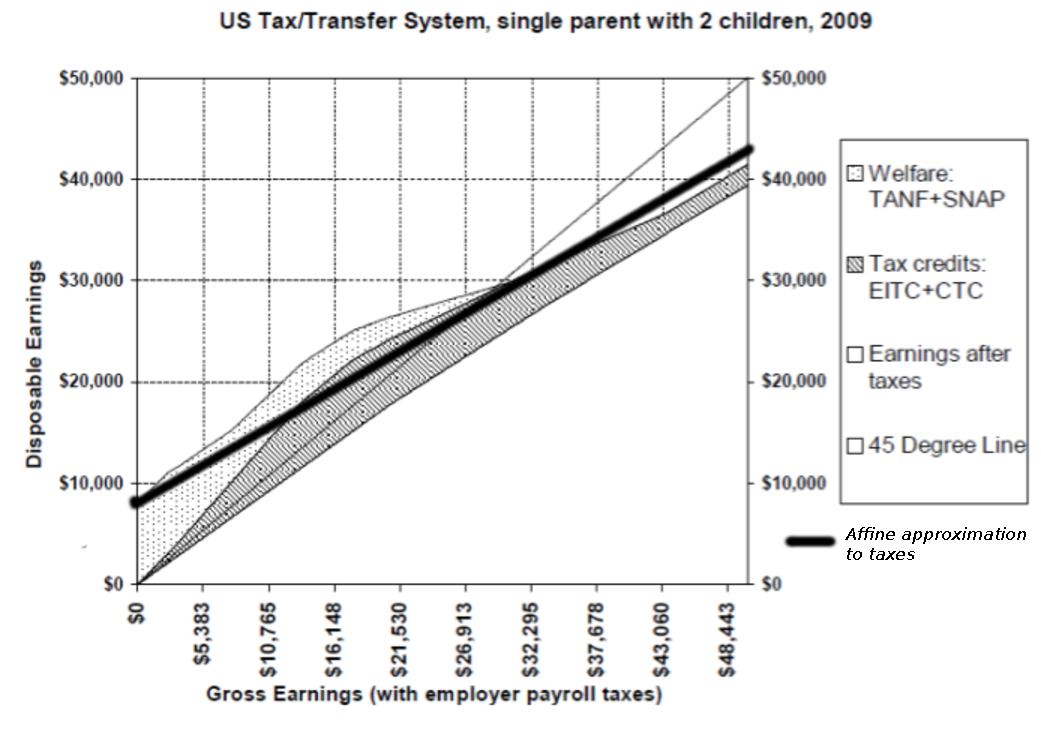
\includegraphics[width=5in,height=3in]{Draft25Graphs/affine_taxes.pdf}
 \caption{ The U.S. tax-transfer system is poorly approximated by a linear function, better by an afine
function.}
 \label{fig:affine_taxes}
 \end{figure}


\subsection{Relationships to literatures}

One a fundamental level our paper is related to both Barro (1974), who showed Ricardian equivalence in a representative agent economy with lump sum taxes, and Barro (1979), who studied the optimal taxation in the same economy when lump sum taxes are ruled out. With incomplete markets and heterogeneity both of the forces uncovered by Barro play role, although the desire for redistribution leads to a richer prescriptions for the optimal policy. 

 A large  literature on Ramsey problems  exogenously rules out transfers in the context of representative agent, general equilibrium models.
  \citet{LucasJr.1983}, \citet{Chari1994},  and AMSS are leading  examples of this approach.
In contrast to those papers, our Ramsey planner cares about redistribution among
agents with different skills and wealths. Other than prohibiting them from depending explicitly
on agent's personal identity, we leave   transfers unrestricted and have the Ramsey planner set
them optimally. Nevertheless, we find that  some of the general principles that emerge from that
representative agent, no-transfers literature continue to hold, in particular, the prescription to
smooth distortions across time and states.  However, it is also true that
allowing the government to set transfers optimally substantially changes
qualitative and quantitative insights about the optimal policy in important respects. 

\footnote{ There is also a more recent strand of literature that focuses on the optimal policy in settings with
heterogeneous agents when a government can impose arbitrary taxes subject only
to explicit informational constraints (see \citet{golosov2007new} for a review). A striking result from that literature
is that when  agent's asset holdings are perfectly observable, the distribution of assets among
agents is irrelevant and an optimal allocation can be achieved purely through
taxation (see, e.g. \citet{Bassetto2004}).  In the previous version of the paper we showed that a mechanism design version of the model with unobservable assets generates some of the similar predictions to the model with affine taxes that we study, in particular, the relevance of net assets and history dependence of taxes. We leave further analysis along this
direction to the  future.}

Several recent papers impute distributive concerns to a Ramsey planner.
Three papers that are perhaps most closely related to ours are \citet{Bassetto1999}, \citet{shin2006ramsey}, and \citet{Wer07a}. Like us, those authors depart from
a representative agent assumption by allowing heterogeneity and considering
distributional consequences of alternative tax and borrowing policies.
The first paper by Bassetto extends the \citet{LucasJr.1983} environment to include $I$ types of
agents who are heterogeneous in their time-invariant labor productivities. There are complete markets and a Ramsey planner  has access only
to proportional taxes on labor income and history-contingent borrowing and
lending. The authors study how the Ramsey planner's vector of Pareto weights
influences how he responds to government expenditures and other shocks by
adjusting the proportional labor tax and government borrowing to cover
expenses while manipulating prices in ways that redistribute wealth between
 `rentiers' (who have low productivities) whose main income is from their asset holdings
and  `workers' (who have high productivities) whose main income source is their labor.

\citet{shin2006ramsey} extends the AMSS economy to have two risk-averse households who
face idiosyncratic income risk. When idiosyncratic income risk is big enough
relative to aggregate government expenditure risk, the Ramsey planner
chooses to issue debt in order to help households engage in precautionary
saving, thereby overturning the AMSS result that  in their quasi-linear case a
 Ramsey planner  eventually sets taxes to zero and lives off its earnings from assets forevermore.
  Shin emphasizes that the
government does this at the cost of imposing tax distortions. While being
confined to proportional labor income taxes and nonnegative
transfers, Shin's Ramsey planner balances two competing self-insurance
motives: aggregate tax smoothing and individual consumption smoothing.

\citet{Wer07a} studies a complete markets economy with heterogeneous agents
and transfers that are unrestricted in sign. He obtains counterparts to our
results about net versus gross asset positions, including that government
assets can be set to zero in all periods. Because he allows unrestricted
taxation of initial assets, the initial distribution of assets plays no
role. Theorem \ref{theorem: main} and its corollaries substantially
generalize Werning's results by showing that all allocations of assets among
agents and the government that imply the same optimal net asset position
lead to the same optimal allocation, a conclusion that holds for market
structures beyond complete markets. \citet{Wer07a} provides an extensive
characterization of optimal allocations and distortions in complete market
economies, while we focus on precautionary savings motives for private
agents and the government that are not present when markets are complete.\footnote{%
\cite{Werning2012} studies optimal taxation with incomplete markets and explores
conditions under which optimal taxes depend only on the aggregate state.}
\footnote{%
More recent closely related papers are \citet{Azzimonti2008,Azzimonti2008a} and \citet{Correia2010}. While these authors study optimal policy in
 economies in which agents are heterogeneous in skills and initial assets, they
  do not allow aggregate shocks.}

  Finally, our numerical analysis in Section \ref{Sec: numerical} is related to a recent paper by McKay and Reis (2013). While the focus of the two papers is very different- McKay and Reis study the effect of calibrated US tax and transfer system on stabilization of output, we focus on the optimal policy responses in a somewhat simpler economy- both papers reach similar conclusions about the importance of transfers and redistribution over business-cycle frequencies.
  
  

\section{Environment\label{Sec: environment}}

\smallskip  %In each period $t\geq 0$, e
Exogenous fundamentals
of the
economy are  functions of a shock  $s_{t}$  that follows an irreducible Markov process, where $s_{t}\in S$ and $S$ is a finite set. We let $s^{t}=\left(
s_{0},...,s_{t}\right) $ denote a history of shocks.

%There are $I$ types of infinitely lived agents.
There is a mass $\pi _{i}$
of a type $i\in I$ agent, with $\sum_{i=1}^{I}\pi _{i}=1.$ Types differ by their skills.
Preferences of an
agent of type $i$ over stochastic processes for consumption $\{c_{i,t}\}_t$
and labor supply $\{l_{i,t}\}_t$ are ordered by
\begin{equation}
\mathbb{E}_{0}\sum_{t=0}^{\infty } \bigl[\Pi_{j=0}^t \beta(s_j)\bigr] U^{i}\left(
c_{i}(s^t),l_{i}(s^t)\right)  \label{utility lifetime}
\end{equation}%
where $\mathbb{E}_{t}$ is a mathematical expectations operator conditioned
on time $t$ information and $\beta(s_t) \in \left( 0,1\right) $ is a state-dependent discount
factor\footnote{We allow the discount factor to depend on the Markov state $s$ to generate flexible  comovement patterns between real interest rates and fundamentals. }. We assume that $l_{i}\in \left[ 0,\bar{l}_{i}\right] $ for some $%
\bar{l}_{i}<\infty .$ Results in section  \ref{sec:Ricardian101} require no
additional assumptions on $U^{i}$ like  differentiability or convexity\footnote{Consequently  our setup allows both extensive and intensive responses of labor.} , but results in later sections do.

An agent of type $i$ who supplies $l_{i}$ units of labor produces $\theta
_{i}\left( s_t\right) l_{i}$ units of output, where $\theta _{i}(s_t)\in \Theta $
is a nonnegative state-dependent scalar. Feasible allocations satisfy
\begin{equation}%\label{eqn:feasiblity}
\sum_{i=1}^{I}\pi_{i}c_{i}(s^t)+g\left( s_{t}\right) =\sum_{i=1}^{I}\pi
_{i}\theta _{i}\left( s_{t}\right) l_{i}(s^t),  \label{feasibility goods}
\end{equation}%
where $g\left( s_{t}\right) $ denotes exogenous government expenditures in
state $s_{t}.$
 We allow $s_t$ to
affect $\beta(s_t)$, government expenditures $g(s_t)$, and the type-specific productivities $\theta_i(s_t)$.

To save on notation, mostly we
use $z_{t}$ to denote a random variable with a time $t$ conditional
distribution that is a function of the history $s^{t}$.
 Occasionally, we use the more explicit notion $z\left(
s^{t}\right) $ to denote a realization  at
a particular history $s^{t}.$

%\textcolor{blue}{From Anmol :  Do we want $ \bigl[\Pi_{j=0}^t \beta(s_j)\bigr] $ or  $\bigl[\Pi_{j=0}^t \beta_j\bigr]$ . If yes, this needs to be modified in a couple of places}

A Ramsey  planner's preferences over a vector of stochastic processes for consumption and
work are ordered by
\begin{equation}
\mathbb{E}_{0}\sum_{i=1}^{I}\pi _{i}\alpha _{i}\sum_{t=0}^{\infty }\bar{\beta}_t U_{t}^{i}\left( c_{i,t},l_{i,t}\right)  \label{govmt objective}
\end{equation}

where the Pareto weights satisfy $\alpha _{i}\geq 0,$ $\sum_{i=1}^{I}\alpha _{i}=1$ and $\bar{\beta}_t=\bigl[\Pi_{j=0}^t \beta_j\bigr]$

In most of this paper, we study an optimal  government policy when agents can   trade
only a one-period risk-free bond.  We assume that the government  imposes an
affine tax
\begin{equation*}
T_t + \tau_t \theta_{i,t}l_{i,t}. \end{equation*}
%We allow the government to choose a feasible sequence of transfers $%
%\{T_{t}\} $.
We do not restrict the sign of $T_{t}$ at any $t$ or $s^t$. %This means that our analysis covers the following example: if
If for some type $i$, $\theta _{i,t}=0$, $b_{i, -1} = 0$ and $U^i$ is defined only on $\mathcal{R}^2_{+}$, his budget constraint will imply that the all feasible allocations for the planner have nonnegative present value of
transfers, since transfers are the sole source of a type $i$ agent's wealth and consumption.

While results in sections \ref{Sec: characterization}, \ref{sec: SteadyStates}, and  \ref{Sec: numerical}  depend on these  assumptions about an affine tax system and incomplete markets,
  key results of  section  \ref{sec:Ricardian101} apply under  more general tax functions and
market structures.

Under an affine tax system, agent $i$'s budget constraint at $t$ is%
\begin{equation}
c_{i,t}+b_{i,t}=\left( 1-\tau _{t}\right) \theta
_{i,t}l_{i,t}+R_{t-1}b_{i,t-1}+T_{t},  \label{agent bc affine}
\end{equation}

\noindent where $b_{i,t}$ denotes asset holdings of a type $i$ agent  at time $t\geq 0$, $%
R_{t-1}$ is a gross risk-free one-period interest rate from  $t-1$ to
 $t$ for $t\geq 1$, and $R_{-1}\equiv 1$. For $t\geq 0$, $R_{t}$ is
measurable with respect to $s^t$. To rule out Ponzi schemes,
we assume that $b_{i,t}$ must be bounded from below. Except in subsection \ref{Sec: extensions}, we
impose no further constraints on agents'  borrowing  and lending. Subsection \ref{Sec: extensions} briefly studies economies with
arbitrary borrowing constraints.

The government budget constraint is%

\begin{equation}
g_{t}+B_{t}=\tau _{t}\sum_{i=1}^{I}\pi _{i}\theta
_{i,t}l_{i,t}-T_{t}+R_{t-1}B_{t-1},  \label{govmt bc affine}
\end{equation}%
where $B_{t}$ denotes the government's assets at time $t$, which we assume
are bounded from below. Our assumptions about preferences
imply that the government can collect only finite revenues in each period, so
this restriction rules out government-run Ponzi schemes.

We assume that private agents and the government start with  assets $%
\{b_{i,-1}\}_{i=1}^{I}$ and $B_{-1}$, respectively.  Asset holdings
satisfy the market clearing condition%

\begin{equation}
\sum_{i=1}^{I}\pi _{i}b_{i,t}+B_{t}=0\text{ for all }t\geq -1.
\label{feasibility bonds}
\end{equation}%
Since $B_{t}$ and all $b_{i,t}$ are bounded from below,  equation (\ref{feasibility bonds}) implies that they are also bounded from above.


Components of  competitive  equilibria are described below

\begin{definition}
\label{Def:components} An \emph{allocation} is a sequence $\left \{
c_{i,t},l_{i,t}\right \} _{i,t}$. An \emph{asset profile} is a sequence $\{
\left \{ b_{i,t}\right \} _{i},B_{t}\}_{t}$. A \emph{price system} is an
interest rate sequence $\{R_{t}\}_{t}$. A \emph{tax policy} is a sequence $%
\{ \tau _{t},T_{t}\}_{t}$.
\end{definition}
%
%We next define a competitive equilibrium. The key feature of that definition
%is that equilibria defined for a given initial assets $\left( \left\{
%b_{i,-1}\right\} _{i},B_{-1}\right) $ and we study the implications of the
%initial assets on the equilibrium allocations.



\begin{definition}
\label{Def: CE with affine taxes}For a given initial asset distribution $\left(
\left \{ b_{i,-1}\right
\} _{i},B_{-1}\right) $, a competitive
equilibrium with affine taxes is a sequence $\{ \left
\{
c_{i,t},l_{i,t},b_{i,t}\right \} _{i},B_{t},R_{t}\}_t$ and a tax policy $%
\left \{ \tau _{t},T_{t}\right
\} _{t},$ %such that the allocation and the
%private components $\left \{b_{i,t}\right \} _{t}$ of the asset profile
%$\left \{ c_{i,t},l_{i,t},b_{i,t}\right \} _{i,t}$
such that $\{ c_{i,t},l_{i,t},b_{i,t} \} _{i,t}$ 
maximize (\ref{utility lifetime})\ subject to (\ref{agent bc affine}) and
$\{b_{i,t}\}_{i,t}$ is bounded; and
constraints (\ref{feasibility goods}), (\ref{govmt bc affine})\ and (\ref%
{feasibility bonds})\ are satisfied.
\end{definition}

%\textcolor{blue}{Each initial asset distribution $\left( \left\{
%b_{i,-1}\right\} _{i},B_{-1}\right) $ is associated with a competitive equilibrium.
%We want to study the effects  of the initial asset distribution on optimal competitive
%equilibrium outcomes.}

%\textcolor{blue}{From Anmol : does the previous sentence belong here ?}

\smallskip Lastly we define optimal competitive equilibria.

\begin{definition}
\label{Def: optimal CE affine} Given $(\{b_{i,-1}\}_{i},B_{-1})$, an
optimal competitive equilibrium with affine taxes is a tax
policy $\left\{ \tau _{t}^{\ast },T_{t}^{\ast }\right\} _{t}$, an allocation
$ \left\{ c_{i,t}^{\ast },l_{i,t}^{\ast } \right\}$, an asset profile
$\left\{\left\{b_{i,t}^{\ast }\right\}
_{i},B_{t}^{\ast }\right\} _{t}$, and a price system $\left\{ R_{t}^{\ast
}\right\} _{t}$ such that (i) given $\left( \left\{ b_{i,-1}\right\}
_{i},B_{-1}\right) $, the tax policy,  %tax-transfer system $\left\{ \tau _{t}^{\ast
%},T_{t}^{\ast }\right\} _{t}$,
 the price system, %$\left\{ R_{t}^{\ast
%}\right\} _{t}$,
and the allocation %$\left\{ \left\{ c_{i,t}^{\ast
%},l_{i,t}^{\ast },b_{i,t}^{\ast }\right\} _{i},B_{t}^{\ast }\right\} _{t}$
constitute a competitive equilibrium; and (ii) there is no other tax policy $%
\left\{ \tau _{t},T_{t}\right\} _{t}$ such that a competitive equilibrium
given $\left( \left\{ b_{i,-1}\right\} _{i},B_{-1}\right) $ and $\left\{
\tau _{t},T_{t}\right\} _{t}$ has a strictly higher value of (\ref{govmt
objective})$.$
\end{definition}

\smallskip We  call $\left \{ \tau _{t}^{\ast },T_{t}^{\ast }\right \}
_{t}$ an \textit{optimal tax policy}, $\{c_{i,t}^{\ast },l_{i,t}^{\ast
}\}_{i,t}$ an \textit{optimal allocation}, and $\left \{ \left \{
b_{i,t}^{\ast }\right \} _{i},B_{t}^{\ast }\right \} _{t}$ an \textit{%
optimal asset profile}.

\section{\protect\smallskip Relevant and Irrelevant Aspects of  the Distribution of Government Debt\label{sec:Ricardian101}}
%
%\textcolor{blue}{Remark from Anmol: Proposition 1 is implied by theorem 1. We can reduce some overlap by starting with the theorem 1 and mentioning Proposition 1 as corollary. I have attempted to reorder the discussion in the section to reflect this}
%\textcolor{red}{Remark from Tom: Anmol, I agree with you very much. Also, much of this section has nothing to do with an {\em optimal}
%equilibrium. I have done some editing to reflect this. I have written an incendiary anti Reinhart-Rogoff first paragraph to this section. }
This section sets forth  a  result that underlies much of the analysis in this paper, namely, that  the level
of government debt is not a state variable for our economy.  The reason is that there is an equivalence class of tax policies and asset profiles that support the same competitive equilibrium allocation.
A competitive  equilibrium allocation pins down only net asset  positions.
The assertions in this section apply to all competitive equilibria, not just the optimal ones that will be our focus in subsequent sections.

%\textcolor{blue}{Do we need a * on the initial conditions in the statement of te theorem. Previously we have used * to denote the optimal competitive equilibrium. I feel that this proof can be re-written without the *}

\begin{theorem}
\label{theorem: main} Given $\left( \left \{ b_{i,-1}\right \}
_{i},B_{-1}\right) $, let $\left \{ \left \{ c_{i,t},l_{i,t},b_{i,t}\right \} _{i},B_{t},R_{t}\right \} _{t} $ and $\left \{ \tau _{t},T_{t}\right
\} _{t}$ be a competitive equilibrium. For any bounded sequences $%
\left \{ \hat{b}_{i,t}\right \} _{i,t\geq -1}$ that satisfy
\begin{equation*}
\hat{b}_{i,t}-\hat{b}_{1,t}=\tilde{b}_{i,t}\equiv b_{i,t}	-b_{1,t}\text{ for all }t\geq -1,i\geq 2,
\end{equation*}%
there exist  sequences $\left \{ \hat{T}_{t}\right \} _{t}$ and $%
\left \{ \hat{B}_{t}\right \} _{t\geq -1}$ that satisfy (\ref{feasibility
bonds}) such that $\left \{ \left \{ c_{i,t},l_{i,t},\hat{b}%
_{i,t}\right \} _{i},\hat{B}_{t},R_{t}\right \} _{t}$ and $\left \{
\tau _{t},\hat{T}_{t}\right \} _{t}$ constitute a competitive
equilibrium given $\left( \left \{ \hat{b}_{i,-1}\right \} _{i},\hat{B}%
_{-1}\right) $.
\end{theorem}

\begin{proof}
Let
\begin{equation}
\hat{T}_{t}=T_{t} + \left(\hat{b}_{1,t} - b_{1,t}\right) -
R_{t-1}\left(\hat{b}_{1,t-1} - b_{1,t-1}\right) \text{ for
all }t\geq 0.  \label{construct That}
\end{equation}%
Given  a tax policy $\left \{ \tau _{t},\hat{T}_{t}\right \} _{t},$ the
allocation $\left \{ c_{i,t},l_{i,t},\hat{b}_{i,t}\right \}
_{t}$ is a feasible choice for consumer $i$ since it satisfies%
\begin{eqnarray*}
c_{i,t}&=&\left( 1-\tau _{t}\right) \theta _{i,t}l_{i,t}+R_{t-1}b_{i,t-1}-b_{i,t}+T_{t}.\\
&=&\left( 1-\tau _{t}\right) \theta _{i,t}l_{i,t}+R_{t-1}\left( b_{i,t-1}-b_{1,t-1}\right) -\left(
b_{i,t}-b_{1,t}\right) +T_{t}+R_{t-1}b_{1,t-1}-b_{1,t} \\
&=&\left( 1-\tau _{t}\right) \theta _{i,t}l_{i,t}+R_{t-1}\left( \hat{b}_{i,t-1}-\hat{b}_{1,t-1}\right) -\left( \hat{b%
}_{i,t}-\hat{b}_{1,t}\right) +T_{t}+R_{t-1}b_{1,t-1}-b_{1,t} \\
 &=&\left( 1-\tau _{t}\right) \theta
_{i,t}l_{i,t}+R_{t-1}\hat{b}_{i,t-1}-\hat{b}_{i,t}+\hat{T}_{t}.
\end{eqnarray*}%
Suppose that $\left \{ c_{i,t},l_{i,t},\hat{b}_{i,t}\right \}
_{t}$ is not the optimal choice for consumer $i$, in the sense that there exists some
other sequence $\left \{ \hat{c}_{i,t},\hat{l}_{i,t},\hat{b}_{i,t}\right \}
_{t}$ that gives strictly higher utility.  Then the choice $%
\left \{ \hat{c}_{i,t},\hat{l}_{i,t},b_{i,t}\right \} _{t}$ is
feasible given the tax rates  $\left \{ \tau _{t},T_{t}\right \} _{t}$%
, which contradicts the assumption that $\left \{ c_{i,t},l_{i,t},b_{i,t}\right \} _{t}$ is the optimal choice for
the consumer given taxes $\left \{ \tau _{t},T_{t}\right \}
_{t}$. The new allocation satisfies all other constraints and
therefore is an equilibrium.
\end{proof}

\smallskip An immediate corollary is  that it is not
total government debt but rather who owns it that affects equilibrium
allocations.

\begin{corollary}
\label{corr: B does not matter} For any pair $B_{-1}^{\prime },B_{-1}^{\prime
\prime }$, there are asset profiles $\left\{ b_{i,-1}^{\prime }\right\} _{i}$ and $%
\left\{ b_{i,-1}^{\prime \prime }\right\} _{i}$ such that
equilibrium allocations starting from  $\left( \left\{ b_{i,-1}^{\prime }\right\}
_{i},B_{-1}^{\prime }\right) $ and  from  $\left( \left\{ b_{i,-1}^{\prime
\prime }\right\} _{i},B_{-1}^{\prime \prime }\right) $ are the same.
%Such sequences $\left\{ b_{i,-1}^{\prime }\right\} _{i}$ and $\left\{
%b_{i,-1}^{\prime \prime }\right\} _{i}$
These asset profiles satisfy%
\begin{equation*}
b_{i,-1}^{\prime }-b_{1,-1}^{\prime }=b_{i,-1}^{\prime \prime
}-b_{1,-1}^{\prime \prime }\text{ for all }i.
\end{equation*}
\end{corollary}
%
%\textcolor{red}{Anmol -- I deleted `optimal' as a modifier of `equilibrium' in the above corollary.}
%\textcolor{blue}{Anmol : I replaced the word ``sequences'' with ``asset profiles''. }


%
%\smallskip These observations  highlight the importance of relative asset
%holdings. Define agents' \textit{net assets positions} $%
%\left\{ \tilde{b}_{i,t}\right\} _{t,i\geq 2}$ as
%\begin{equation*}
%\tilde{b}_{i,t}=b_{i,t}-b_{1,t}\text{ for all }t\geq -1,i\geq 2.
%\end{equation*}

\smallskip
This result is closely related to Ricardian Equivalence in \citet{Barro1974}. There are however some important distinctions. In Barro's representative agent model lump sum taxes are not distortionary. In our economy, since the planner does not have person-specific taxes, a lump sum transfer introduces distortions in inequality and as we will see in following sections this force has a significant effect on optimal policy. Despite this, Ricardian equivalence continues to hold.\footnote{%
\citet{Wallace1981}'s Modigliani-Miller theorem for a class of government open
market operations has a similar flavor. \citet{sargent1987dynamic} describes the
structure of a set of related Modigliani-Miller theorems for government
finance.} %\textcolor{red}{Anmol: I deleted the phrase ` in the optimum'. And I deleted `optimal'
%from a couple places in the following section.  The argument doesn't depend on the equilibria being optimal.}
Theorem \ref{theorem: main} shows that many different transfer
sequences $\left\{ T_{t}\right\} _{t}$ and asset profiles $\left\{
b_{i,t},B_{t}\right\} _{i,t}$  support the same  equilibrium allocation.
For example, one can set government assets $B_{i,t}=0$ without loss of
generality.
%Theorem \ref{theorem: main} shows that the underlying economic mechanisms will
%generally be quite different from those in  representative agent economies
%in which restrictions on a government's ability to borrow and lend significantly affect
%optimal equilibrium outcomes, e.g. AMSS or Faraglia et al.\ (2012).
Alternatively,  we can normalize  assets $b_{i,t}$ of any type $i$.

Theorem \ref{theorem: main} continues to hold in more general environments. For example, we could allow
agents to trade all  Arrow securities and still show that  equilibrium
allocations depend only on agents' net assets positions.
Similarly, our results   hold in  economies with capital.
% In section \ref{Sec: extensions-NDPF},  we explore outcomes when a government has
% access to more general taxes, for example, of a form $T_{t}(y_{t})$ or $%
% T_{t}(y_{t},...,y_{0})$. While those richer  tax systems  allow better redistribution and
% smaller distortions, they do not affect  the conclusions of theorem \ref{theorem: main}.
% 

\subsection{Extension : Borrowing constraints}\label{Sec: extensions}
%\textcolor{blue}{Anmol : I have removed proposition 2 and addeda mention that the corollary to theorem 1 is valid under adhoc borrowing constraints too. We dont have anything more to say about it. }
%
%\textcolor{blue}{Anmol : I have attempted to re-write the appendix in a way that it is self-contained. The earlier one had forward references and missing arguments.}

Representative agent models  rule out  Ricardian equivalence
either  by assuming distorting taxes or by imposing ad hoc borrowing constraints. %In section \ref{sec:Ricardian101},
By way of contrast, we have verified that Ricardian equivalence holds in our economy even though
there are distorting taxes. % are typically part of an optimal equilibrium.
Imposing ad-hoc borrowing limits also leaves Ricardian equivalence intact in our economy.\footnote{%
\citet{Bryant1984} describe how a government can use borrowing
constraints as part of a welfare-improving policy to finance exogenous
government expenditures.\citet{Sargent1987} describe Modigliani-Miller
theorems for government finance in a collection of economies in which
borrowing constraints on classes of agents produce the kind of rate of
return discrepancies that Bryant and Wallace manipulate.} In economies with
exogenous borrowing constraints, agents' maximization problems  include the
additional constraints
\begin{equation}
b_{i,t}\geq \underline{b}_{i}  \label{borrowing constraint}
\end{equation}%
for some exogenously given $\left\{ \underline{b}_{i}\right\} _{i}.$ %We
%define an equilibrium similarly to Definition \ref{Def: CE with affine taxes}%
\begin{definition}
\label{Def: CE with affine taxes borrowing constraints}For given $\left(
\left \{ b_{i,-1},\underline{b}_{i}\right \} _{i},B_{-1}\right) $ and $%
\left
\{ \tau _{t},T_{t}\right \} _{t},$ a competitive equilibrium with
affine taxes and exogenous borrowing constraints is a sequence $\{ \left \{
c_{i,t},l_{i,t},b_{i,t}\right \} _{i},B_{t},R_{t}\}_{t} $ such that $%
\left
\{ c_{i,t},l_{i,t},b_{i,t}\right \} _{i,t}$ maximizes (\ref{utility
lifetime})\ subject to (\ref{agent bc affine}) and (\ref{borrowing
constraint}), $\{ b_{i,t} \}_{i,t}$ are bounded,
and constraints (\ref{feasibility goods}), (\ref{govmt bc affine})\ and (\ref%
{feasibility bonds})\ are satisfied.
\end{definition}

We can define an \emph{optimal} competitive equilibrium with exogenous borrowing
constraints by extending Definition \ref{Def: optimal CE affine}.

%The role of the initial distribution of assets  is
%unaffected by the introduction of the ad-hoc debt limits and  so is Corollary  \ref{corr: B does not matter}.
The introduction of the ad-hoc debt limits leaves unaltered the conclusions of  Corollary  \ref{corr: B does not matter} and
the role of the initial distribution of assets across agents.
 The next proposition asserts
that ad-hoc borrowing limits do not limit a government's ability to respond to
aggregate shocks.\footnote{%
See \citet{Yared2012,Yared2013}  who shows a closely related result.}
\smallskip

\begin{proposition}
\label{thm:borrowing_constraint}  Given an initial asset distribution $\left(
\left\{ b_{i,-1}\right\} _{i},B_{-1}\right)$, let $\left\{ c_{i,t},l_{i,t}\right\} _{i,t}$ and $\left\{ R_{t}\right\}_t $ be a competitive
equilibrium allocation and interest rate sequence in an economy without
exogenous borrowing constraints. Then for any exogenous
constraints $\left\{ \underline{b}_{i}\right\} _{i}$, there is a government
tax policy $\left\{ \tau _{t},T_{t}\right\} _{t}$ such that $\left\{
c_{i,t},l_{i,t}\right\} _{i,t}$ is a competitive equilibrium
allocation in an economy with exogenous borrowing constraints $\left(
\left\{ b_{i,-1},\underline{b}_{i}\right\} _{i},B_{-1}\right) $ and $\left\{
\tau _{t},T_{t}\right\} _{t}.$
\end{proposition}

\begin{proof}
Let $\left\{ c_{i,t},l_{i,t},b_{i,t}\right\} _{i,t}$
be a competitive equilibrium allocation without exogenous borrowing
constraints. Let $\Delta _{t}\equiv \max_{i}\left\{ \underline{b}%
_{i}-b_{i,t}\right\} .$ Define $\hat{b}_{i,t}\equiv b_{i,t}+\Delta _{t}$ \ for all $t\geq 0$ and $\hat{b}_{i,-1}=b_{-1}.$ By Theorem %
\ref{theorem: main}, $\left\{ c_{i,t},l_{i,t},\hat{b}%
_{i,t}\right\} _{i,t}$ is also a competitive equilibrium allocation without
exogenous borrowing constraints. Moreover, by construction $\hat{b}_{i,t}-%
\underline{b}_{i}=b_{i,t}+\Delta _{t}-\underline{b}_{i}\geq 0$.
Therefore, $\hat{b}_{i,t}$ satisfies (\ref{borrowing constraint}). Since
agents' budget sets are smaller in the economy with exogenous borrowing
constraints, and $\left\{ c_{i,t},l_{i,t},\hat{b}%
_{i,t}\right\} _{i,t}$ are feasible at interest rate process $\left\{
R_{t}\right\} _{t}$, then $\left\{ c_{i,t},l_{i,t},%
\hat{b}_{i,t}\right\} _{i,t}$ is also an optimal choice for agents in the
economy with exogenous borrowing constraints $\left\{ \underline{b}%
_{i}\right\} _{i}.$ Since all market clearing conditions are satisfied, $%
\left\{ c_{i,t},l_{i,t},\hat{b}_{i,t}\right\} _{i,t}$ is a
competitive equilibrium allocation and asset profile.
\end{proof}

To explore the intuition underlying Proposition \ref{thm:borrowing_constraint}, suppose to the contrary that the exogenous borrowing constraints  restricted a  government's
 ability to achieve a desired allocation. That  means that
the government would want to increase  its borrowing
and to repay agents later, which the borrowing constraints prevent. But the government can just reduce
transfers today and increase them tomorrow. That would  achieve the  desired  allocation
without violating the exogenous borrowing constraints.

Welfare can  be strictly higher in an economy  with exogenous
borrowing constraints  because  a government might want to
push some agents against their borrowing limits. When some agents' borrowing
constraints bind, their shadow interest rates differ from the
common interest rate that unconstrained agents face. When the government rearranges tax
policies to  affect the  interest rate, it affects constrained and unconstrained agents
 differently.  By facilitating
redistribution, this can improve welfare. %In the next several paragraphs, we will formalize this
%intuition.
In appendix \ref{appndx: borrowing constraints example}, we construct an example without any
shocks in which the government can achieve higher welfare by using borrowing
constraints to improve its ability to redistribute.
% \subsection{Extension 2: More general taxes \label{Sec: extensions-NDPF}}
% %\textcolor{red}{From Tom:I have edited this section }
% 
% The conclusions  of theorem \ref{theorem: main} also apply in settings typical in  a New Dynamic Public Finance (NDPF)  literature that studies taxes and other arrangements that  decentralize an optimal allocation that respects information gaps between agents and a government.\footnote{%
% For surveys, see \citet{golosov2007new} and \cite{kocherlakota2010new}.}
% Thus, consider an economy where agents' skills $\theta$ are private information (and do not change over time).  Suppose
% that the government observes output $y\equiv \theta l$ and $c$ for each
% agent. Constrained optimal allocations solve the mechanism design problem
% %\textcolor{red}{From Tom: I have allowed stochastic discount favors.}
% \begin{equation}
% \max_{\left \{ c_{i,t},y_{i,t}\right \} }\mathbb{E}_{0}\sum_{i=1}^{I}\alpha
% _{i}\pi _{i}\sum_{t=0}^{\infty } \bigl[\Pi_{j=0}^t \beta(s_j)\bigr] U^{i}\left( c_{i,t},\frac{y_{i,t}}{%
% \theta _{i}}\right)  \label{mechdes max}
% \end{equation}%
% subject to incentive constraints%
% \begin{equation}
% \mathbb{E}_{0}\sum_{t=0}^{\infty }\bigl[\Pi_{j=0}^t \beta(s_j)\bigr]U^{i}\left( c_{i,t},\frac{y_{i,t}%
% }{\theta _{i}}\right) \geq \mathbb{E}_{0}\sum_{t=0}^{\infty }\bigl[\Pi_{j=0}^t \beta(s_j)\bigr]\left( c_{j,t},\frac{y_{j,t}}{\theta _{i}}\right) \text{ for all }%
% i,j  \label{mechdes IC}
% \end{equation}%
% and the feasibility constraint%
% \begin{equation}
% \sum_{i=1}^{I}\pi _{i}c_{i,t}+g_{t}=\sum_{i=1}^{I}\pi _{i}y_{i,t}.
% \label{mechdes feas}
% \end{equation}%
% Let $\left \{ c_{i,t}^{sp},y_{i,t}^{sp}\right \} _{i,t}$ be the optimal allocation. To implement the optimal allocation
% in a competitive equilibrium, we allow a general
% non-linear tax schedule $T_{t}\left( y_{t},X_{t}\right) $, where $X_{t}$ is a vector
% of  agent-specific variables like past labor earnings.\footnote{It is easy to see that the optimal allocation is \emph{history independent}. We can rewrite the mechanism design problem as
% % (\ref{mechdes max}) as%
% \begin{equation*}
% \max_{\left \{ c_{i,t},y_{i,t}\right \} }\min_{\left \{ \eta _{ij}\right \} }%
% \mathbb{E}_{0}\sum_{i=1}^{I}\sum_{t=0}^{\infty } \bigl[\Pi_{j=0}^t \beta(s_j)\bigr]\left\{\left( \alpha _{i}\pi _{i}+\eta
% _{i,i}\right) U^{i}\left( c_{i,t},\frac{y_{i,t}}{\theta _{i}}\right)
% -\sum_{j\neq i}\eta _{j,i}U^{j}\left( c_{j,t},\frac{y_{j,t}}{\theta _{i}}%
% \right)\right\}
% \end{equation*}%
% subject to (\ref{mechdes feas}). This problem is equivalent to a sequence of
% static problems for each realization of $g_{t}.$
% Appendix \ref{apndx: unobs-assets} constructs an example that shows if, in addition, agents' assets are also unobservable, then optimal allocations are history dependent}
% 
% We assume that agents begin with initial debt
% holdings $\left \{ b_{i,-1}\right \} _{i}$ and that each period they can
%  trade a one-period risk-free bond with gross return $\{R\}_t$. An
% agent's budget constraint is the same as (\ref{agent bc affine}),  except that now
% $-T_{t}+\tau y_{t}$ is replaced by $T_{t}\left( y_{t},X_{t}\right) .$ We
% modify the definition of a competitive equilibrium with these more general
% taxes in the natural way.
% 
% Debt plays no significant role, because  if his debt differs from zero, the government
% can tax away \textit{all} of an agent's income
% from assets by setting $T_{t}\left( y_{t},b_{t-1},F\left( \left \{
% y_{s}\right \} _{s=0}^{t-1}\right) \right) =y_{t}+\max \left \{
% R_{t}b_{t},0\right \} $ if $b_{t}\neq 0.$
% 
% Thus,  in this economy,  a much stronger version of theorem \ref{theorem: main} emerges.%
% \footnote{%
% See also a related result of \citet{Bassetto2004}, who showed
% that when taxes can depend on past labor income, the path of government debt
% is indeterminate.}
% 
% \begin{corollary}
% Any sequence of assets $\left \{ b_{i,t}\right \} _{i,t}$ is a part of an
% optimal competitive equilibrium allocation for some optimal non-linear tax $%
% T_{t}\left( y_{t},b_{t-1},F\left( \left \{ y_{s}\right \}
% _{s=0}^{t-1}\right) \right) .$
% \end{corollary}
% This conclusion is sensitive to the presumption that the private information pertains only  to agent's skills. Appendix \ref{apndx: unobs-assets} shows that if in addition, agents assets are also unobservable, then theorem \ref{theorem: main} can still be recovered in the sense that only \emph{net} positions matter.
% 
\subsection{Ricardian irrelevance and optimal equilibria}

Our statements about Ricardian irrelevance apply to all competitive equilibrium allocations,
not just the optimal ones that are the main focus of this paper.
To appreciate how  these  Ricardian irrelevance results affect optimal equilibria, suppose that we increase an
initial level of government debt from $0$ to some arbitrary level $%
B_{-1}^{\prime } > 0$. If the government were to hold transfers $\left\{ T_{t}\right\} _{t}$ fixed, it would
 have  to increase  tax rates $\left\{ \tau
_{t}\right\} _{t}$ enough to collect a present value of revenues sufficient to
repay $B_{-1}^{\prime }$. Since deadweight losses are convex in $\tau ,$
higher levels of debt financed with bigger distorting taxes $\{\tau_t\}$  impose larger
distortions on the economy, thereby degrading the equilibrium allocation.  But this would not happen  if
the government were instead  to adjust transfers in response to a higher initial debt. To determine optimal transfers, we need to
know who owns  the initial government debt $B_{-1}^{\prime }$. For example, suppose that agents hold equal amounts of it. Then
each unit of debt repayment achieves the same redistribution as one
unit of transfers. If the original tax policy  at $B_{-1}^{\prime } =0 $ were optimal, then  the best policy for a government with  initial debt $%
B_{-1}^{\prime } >0 $ would be to reduce the present value  transfers by exactly the amount of the
increase in per capita debt, because then distorting taxes $\left\{ \tau
_{t}\right\} $ and the allocation would both remain unchanged.\footnote{This example illustrates
principles proclaimed by Simon \citet[p. 85]{newcomb1865critical} in the quotation with
which we began this paper.}

But the situation would be different if  holdings of government
debt were not equal across agents. For example, suppose  that  richer people owned disproportionately more government debt
than poorer people. That would mean that inequality
is  effectively initially  higher in an economy with higher initial government debt. As a result, a
government with Pareto weights $\{\alpha_i\}$ that favor equality would want to increase both  distorting  tax rates $\left\{ \tau _{t}\right\} $
and transfers $\left\{ T_{t}\right\} $ to offset the increase in inequality
associated with the increase in government debt. The conclusion would be the
opposite if government debt were to be  owned mostly by poorer
households.



This logic shows how important it is to know the distribution of government debt across people. Government debt that is widely distributed across households
(e.g., implicit Social Security debt) is less distorting than
 government debt owned mostly by people whose incomes are at the top of the income
distribution (e.g., government debt held by hedge funds).\footnote{%
It is straightforward to extend our analysis to open economy with foreign
holdings of domestic debt. The more government debt is owned by the
foreigners, the higher are the distorting taxes that  the government  needs to
impose.}

\section{Quasi-linear preferences}\label{Sec: quasilinear}
Before we use section \ref{Sec: characterization}  for general characterization of our problem, in this section we study a special case of our economy that allows us to get a long way analytically and to identify some forces that drive outcomes. In particular we assume that the only source of aggregate shocks is the fluctuation in $g_t$ and preferences are given by $U^{i}\left( c,l\right) =c-h_{i}(l)$ where $h_{i}$ is an increasing differentiable function with $h_{i}^{\prime
}\left( 0\right) =0$ and $h_{i}^{\prime }\left( \bar{l}_{i}\right) =\infty $. These quasi-linear preferences have been extensively studied in the context of representative agent economies (see, e.g.,  AMSS, \cite{Farhi2010}, \cite{Battaglini2007,Battaglini2008}, \cite{Yared2012}, \cite{Faraglia2011}). We pursue two goals in this section. First, this economy provides a stark contrast of the optimal policy in our economy when transfers are chosen optimally with representative agent models in which the choice of transfers is exogenously restricted. Second, this set up switches off two channels which are present more generally, namely, that the marginal utilities of agents are differently affected by changes in transfers and that the interest rate in general is not constant. These two forces will play an important role in determining the long run allocations in Section \ref{sec: SteadyStates}

To simplify notation, we now assume that the initial debt is $%
\left\{ \beta ^{-1}b_{i,-1}\right\} _{i}.$

\begin{proposition}
\label{Prop: quasilinear} Suppose that preferences are quasi-linear and the only aggregate shocks are $g_t$. Then the optimal tax rate $\tau
_{t}^{\ast }$ satisfies $\tau _{t}^{\ast }=\tau ^{\ast }$. An optimum asset
profile $\left \{ b_{i,t}^{\ast },B_{t}^{\ast }\right \} _{i,t}$ can be
chosen to satisfy $b_{i,t}^{\ast }=b_{i,-1}$ for all $i,\ t\geq 0$ and $%
B_{t}^{\ast }=B_{-1}$ for all $t\geq 0$.\footnote{%
We thank Guy Laroque for suggesting the idea for this proof.}
\end{proposition}

\begin{proof}
When preferences are quasilinear, the interest rate $R_{t}=\beta
^{-1}$ for all $t$ and % the necessary condition for compatitive equilirbium
%is
$\left( 1-\tau _{t}\right) \theta _{i}=h_{i}^{\prime }(l_{i,t})$ for all $%
t.$ For our purposes, it is more convenient to express the labor supply
component of the allocation as a function of $\left( 1-\tau \right) $ and
optimize with respect to $\tau $ rather than $\left\{ l_{i}\right\} _{i}.$
We  invert  $h_{i}^{\prime }(\cdot )$ to express labor supply $%
l_{i}$ as a function of $\left( 1-\tau \right) .$ Call this function $%
H_{i}\left( 1-\tau \right) $. Use the budget
constraint (\ref{agent bc affine}) to obtain
\begin{equation}
c_{i,t}+b_{i,t}-\left( 1-\tau _{t}\right) H_{i}\left( 1-\tau _{t}\right)
=T_{t}+\beta ^{-1}b_{i,t-1}.  \label{affine imp quasi}
\end{equation}%
The optimal allocation solves
\begin{equation}
\max_{\left\{ c_{i,t},b_{i,t},\tau_t,T_{t}\right\} _{i,t}}\mathbb{E}%
_{0}\sum_{t=0}^{\infty }\sum_{i=1}^{I}\alpha _{i}\pi _{i}\beta ^{t}\left[
c_{i,t}-h_{i}\left( H_{i}\left( 1-\tau_t \right) \right) \right]
\label{AMSS max}
\end{equation}%
subject to $\left\{ b_{i,t}\right\} _{i,t}$ being bounded, (\ref{affine imp
quasi}), and
\begin{equation*}
\sum_{i=1}^{I}\pi _{i}c_{i,t}+g_{t}=\sum_{i=1}^{I}\pi _{i} H_{i}\left( 1-\tau _{t}\right) .
\end{equation*}%
Note that since $\left\{ b_{i,t}\right\} _{i,t}$ is bounded,
\begin{equation*}
\mathbb{E}_{0}\sum_{t=0}^{\infty }\beta ^{t}\left[ \beta
^{-1}b_{i,t-1}-b_{i,t}\right] =\beta ^{-1}b_{i,-1}+\lim_{\mathcal{T}%
\rightarrow \infty }\mathbb{E}_{0}\left( \sum_{t=0}^{\mathcal{T}}\beta ^{t}%
\left[ b_{i,t}-b_{i,t}\right] -\beta ^{\mathcal{T}+1}b_{i,\mathcal{T}%
+1}\right) =\beta ^{-1}b_{i,-1}.
\end{equation*}%
Use (\ref{affine imp quasi}) to eliminate $c_{i,t}$ and then use  the preceding
expression  to get
\begin{equation}
\max_{\left\{ b_{i,t},\tau _{t},T_{t}\right\} _{i,t}}\mathbb{E}%
_{0}\sum_{t=0}^{\infty }\sum_{i=1}^{I}\alpha _{i}\pi _{i}\beta ^{t}\left[
T_{t}+\left( 1-\tau _{t}\right) H_{i}\left( 1-\tau _{t}\right) -h_{i}\left(
H_{i}\left( 1-\tau_t \right) \right) \right] +\beta
^{-1}\sum_{i=1}^{I}b_{i,-1}.  \label{quasilinear max}
\end{equation}%
subject to
\begin{equation}
\sum_{i=1}^{I}\pi _{i}\left[ T_{t}+\beta ^{-1}b_{i,t-1}-b_{i,t}+\left(
1-\tau _{t}\right) H_{i}\left( 1-\tau _{t}\right) \right] +g_{t}=%
\sum_{i=1}^{I}\pi _{i}H_{i}\left( 1-\tau _{t}\right) .
\label{quasilinear feasibility}
\end{equation}%
Let $\beta ^{t}\lambda _{t}$ be the Lagrange multiplier on the time $t$
feasibility constraint \eqref{feasibility goods}. The first-order condition with respect to $T_{t}$
implies that $\lambda _{t}=\sum_{i=1}^{I}\alpha _{i}\pi _{i}$ is constant
and independent of $t.$ Therefore, optimal taxes $\tau _{t}=\tau^{\ast }$ are
also constant and independent of $t.$  Using $\tau^{\ast}$, equation (\ref{quasilinear feasibility}) pins down $\sum_{i=1}^{I}\pi _{i}\left[ T_{t}+\beta ^{-1}b_{i,t-1}-b_{i,t}\right]$. Without loss of generality we can set $b^*_{i,t}=b_{i,-1}$ and $T^*_t$ to satisfy  (\ref{quasilinear feasibility}). %The last part of the Proposition
%follows from Theorem \ref{theorem: main}.
\end{proof}

\smallskip In the optimal equilibria for the quasi-linear economy described in Proposition \ref{Prop: quasilinear}, fluctuations in lump-sum taxes and
transfers ``do all the work''. In period 0, the government chooses an optimal
present value of transfers and a constant tax rate that pays for it. Tax rates  and transfers depend on the Pareto weights $\left\{ \alpha
_{i}\right\} $:  higher Pareto weights on low skilled agents imply
higher transfers and tax rates. In response to a shock $g_{t}$, the
government adjusts transfers in period $t$ by the amount of the shock. Since
all agents are risk-neutral,  welfare is unaffected by
fluctuations in transfers. This allows the government  to  perfectly smooth distorting tax rates.

\smallskip

\subsubsection{Comparison with representative agent economies} \label{sec: comp with AMSS}

The \cite{LucasJr.1983} and AMSS representative agent models
impose $T_{t}\geq 0$. An informal justification behind doing so is the desire of the government to not hurt poor agents, who might be unable to afford lump-sump taxes.  This constraint always binds in the Lucas and Stokey
model and that binds in the AMSS model  until the government has acquired enough
assets to finance all future expenditures from earnings on those assets. In those
representative agent models, the government would like to impose lump-sum \emph{taxes}, not
transfers. We explicitly model redistributive concerns by imputing Pareto weights to heterogeneous agents and obtained very different dynamics as shown in Proposition \ref{Prop: quasilinear}. In this section we argue that the differences in the dynamics come from the presence of this arbitrary restrictions on transfers and not explicit or implicit redistributory motives. 

We impose  the following in our maximization problem (\ref{AMSS max}), namely\footnote{This makes AMSS a special case of our economy },
\begin{equation}
T_{t}\geq 0\text{ for all }t.  \label{T ge 0}
\end{equation}%


The following proposition states it is optimal for the planner to set policy in such a way that constraint \eqref{T ge 0} becomes slack overtime\footnote{It can be shown that if $g$ is not too high and government is sufficiently redistributory (i.e $\alpha_i$ is sufficiently high for low productivity agents), constraints (\ref{T ge 0}) is \emph{always} slack.}.
\smallskip
\begin{proposition}\label{prop:AMSS_killer1}
Assume that $I \geq 1$ and $g_t$ takes more than one value. Let $\beta ^{t}\chi _{t}$ be the Lagrange multiplier on constraint (\ref{T
ge 0}) in a version of  maximization problem (\ref{AMSS max}) that is augmented with constraint (\ref{T
ge 0}). Then $\chi _{t}\rightarrow
0 $ a.s.
\end{proposition}

\begin{proof}
\smallskip Our augmented version of the maximization problem (\ref{AMSS max}) can be expressed
as maximization problem (\ref{quasilinear max})\ with an additional
constraint (\ref{T ge 0}). The first-order conditions for $T_{t}$ yield $%
\sum_{i=1}^{I}\alpha _{i}\pi _{i}=$ $\mu _{t}+\chi _{t}$, while the
first-order condition for $b_{i,t}$ implies $\mu _{t}=\mathbb{E}%
_{t}\mu _{t+1}.$ Since $\chi _{t}\geq 0,$ these two conditions imply
that $\chi _{t}$ is a nonnegative martingale and therefore $\chi _{t}$ must
almost surely converge to a constant. This, in turn, implies that $\mu _{t}$ must
almost surely converge to a constant. Then the first-order conditions for $\tau _{t}$
also imply that $\tau _{t}$ must converge a.s. to some $\tau ^{\ast }.$

Suppose $\chi _{t}\rightarrow \chi ^{\ast }>0.$ This implies that $%
T_{t}\rightarrow 0$ and (\ref{quasilinear feasibility}) becomes
\begin{equation*}
-\beta ^{-1}B_{i,t-1}+B_{i,t}+\sum_{i=1}^{I}\pi _{i}\left( 1-\tau ^{\ast
}\right) H_{i}\left( 1-\tau ^{\ast }\right) +g_{t}=\sum_{i=1}^{I}\pi
_{i}H_{i}\left( 1-\tau ^{\ast }\right) ,
\end{equation*}%
where we used (\ref{feasibility bonds}) to substitute for $\sum_{i=1}^{I}\pi
_{i}b_{i,t}.$ If $g_{t}$ can take more than one value and follows an irreducible
Markov process, then for any bound on $B_{t}$, we can find a sequence of
government expenditures $g_{t}$ for which this bound will eventually be
violated, leading to a contradiction. This implies that $\chi
_{t}\rightarrow 0.$
\end{proof}

Proposition \ref{Prop: quasilinear} emphasized that in absence of (\ref{T ge 0}) the government uses flutuations in transfers to finance all fluctuations in expenditures.  Constraint \ref{T ge 0} imposes an asymmetry in using transfers to smooth fluctuations in expenditures. Around zero it is costless to increase transfers by a small amount but infinitely more costly to decrease them by the same amount. This forces the optimal policy to engineers taxes and assets that allows the economy to eventually grow out this constraint. 
% 
% 
% \smallskip Proposition \ref{Prop: quasilinear} and \ref{prop:AMSS_killer1} shed light on  the key force that
% drives asymptotic outcomes in  AMSS for quasi-linear
% preferences. Although constraint \eqref{T ge 0} need not bind in $I>1$ economies like ours, when $I=1$ it almost \emph{always} binds. %\footnote{%
% %The exception is after the first-best outcome is eventually achieved in AMSS
% %when the government has accumulated a   stock of assets sufficiently large to
% %finance all subsequent expenditures.}
%  Since the risk-free interest rate equals the
% discount rate, a Ramsey planner %who faces constraint \eqref{T ge 0}
% saves partly  to relax future constraints (\ref{T ge 0}), a
% motive that endures until the planner has saved enough to render  slack all future
% constraints \eqref{T ge 0}. Distortionary taxes $\tau^*_t$ are asymptotically zero.
% %In the representative agent economy of
% %AMSS with quasi-linear preferences, constraint (\ref{T ge 0}) binds  until the government has
% %acquired enough assets that it never again has to set the tax rate $\tau_t >0$. %This explains the AMSS (2002) result that the government
% %collects no taxes in the long run.
% %\textcolor{green}{David: I've edited the last sentence to read as follows: }
% 
% 
% In contrast, if the restriction that $T_t \geq 0$ is imposed when agents are heterogeneous and the
% government cares about redistribution,  the government will reallocate assets across  heterogeneous agents until the constraint $T_t \geq 0$ never again binds.  After that, the tax rate will typically be positive and the
% continuation allocation will not be  first-best, in contradiction to the AMSS limiting outcome with quasi-linear preferences.
%\textcolor{red}{From Tom:  I have divided and edited the previous two sentences -- rewritten from David's last version.}

For quasi-linear preferences, figure \ref{fig: AMSS vs BEGS} compares equilibrium dynamics in a
representative agent (AMSS) economy and an economy with two agents, one who
is not productive, and  Pareto weights chosen to make
transfers be positive at all times  and along all  histories. The sequences of $s_t$ shocks are identical across the two economics.
 While tax rates converge to zero for the AMSS economy, they are constant for the heterogeneous agent economy.\footnote{The plots for the AMSS and the heterogeneous agent economies are both  for quasi-linear preferences with a Frisch elasticity of labor equals 0.5 and a discount factor $\beta=0.95$. In the AMSS economy,  the agent's  initial assets are zero  and  government expenditure shocks $g(s_t) \in\{.1,.3\}$ are generated using an IID process with equally likely outcomes.  For the heterogeneous agent economy, we set  $\alpha_2=.54$ so that the initial labor taxes are similar to those for the AMSS economy}. %The code is available at https://github.com/dgevans/AMSS.git.}
%\textcolor{blue}{Anmol : Remove the words BEGS from the label. Also make sure that both the lines start as mentioned in the footnote .}
%\FRAME{ftbpFU}{5.0298in}{2.5892in}{0pt}{\Qcb{Taxes in AMSS (solid line) and
%heterogeneous agent economy (dotted line) with quasi-linear preferences}}{%
%\Qlb{fig: AMSS vs BEGS}}{begs_amss.eps}{\special{language "Scientific
%Word";type "GRAPHIC";maintain-aspect-ratio TRUE;display "USEDEF";valid_file
%"F";width 5.0298in;height 2.5892in;depth 0pt;original-width
%20.0074in;original-height 10.2454in;cropleft "0";croptop "1";cropright
%"1";cropbottom "0";filename 'Draft25Graphs/BEGS_AMSS.eps';file-properties
%"XNPEU";}}



  \begin{figure}[htp]
 \centering
 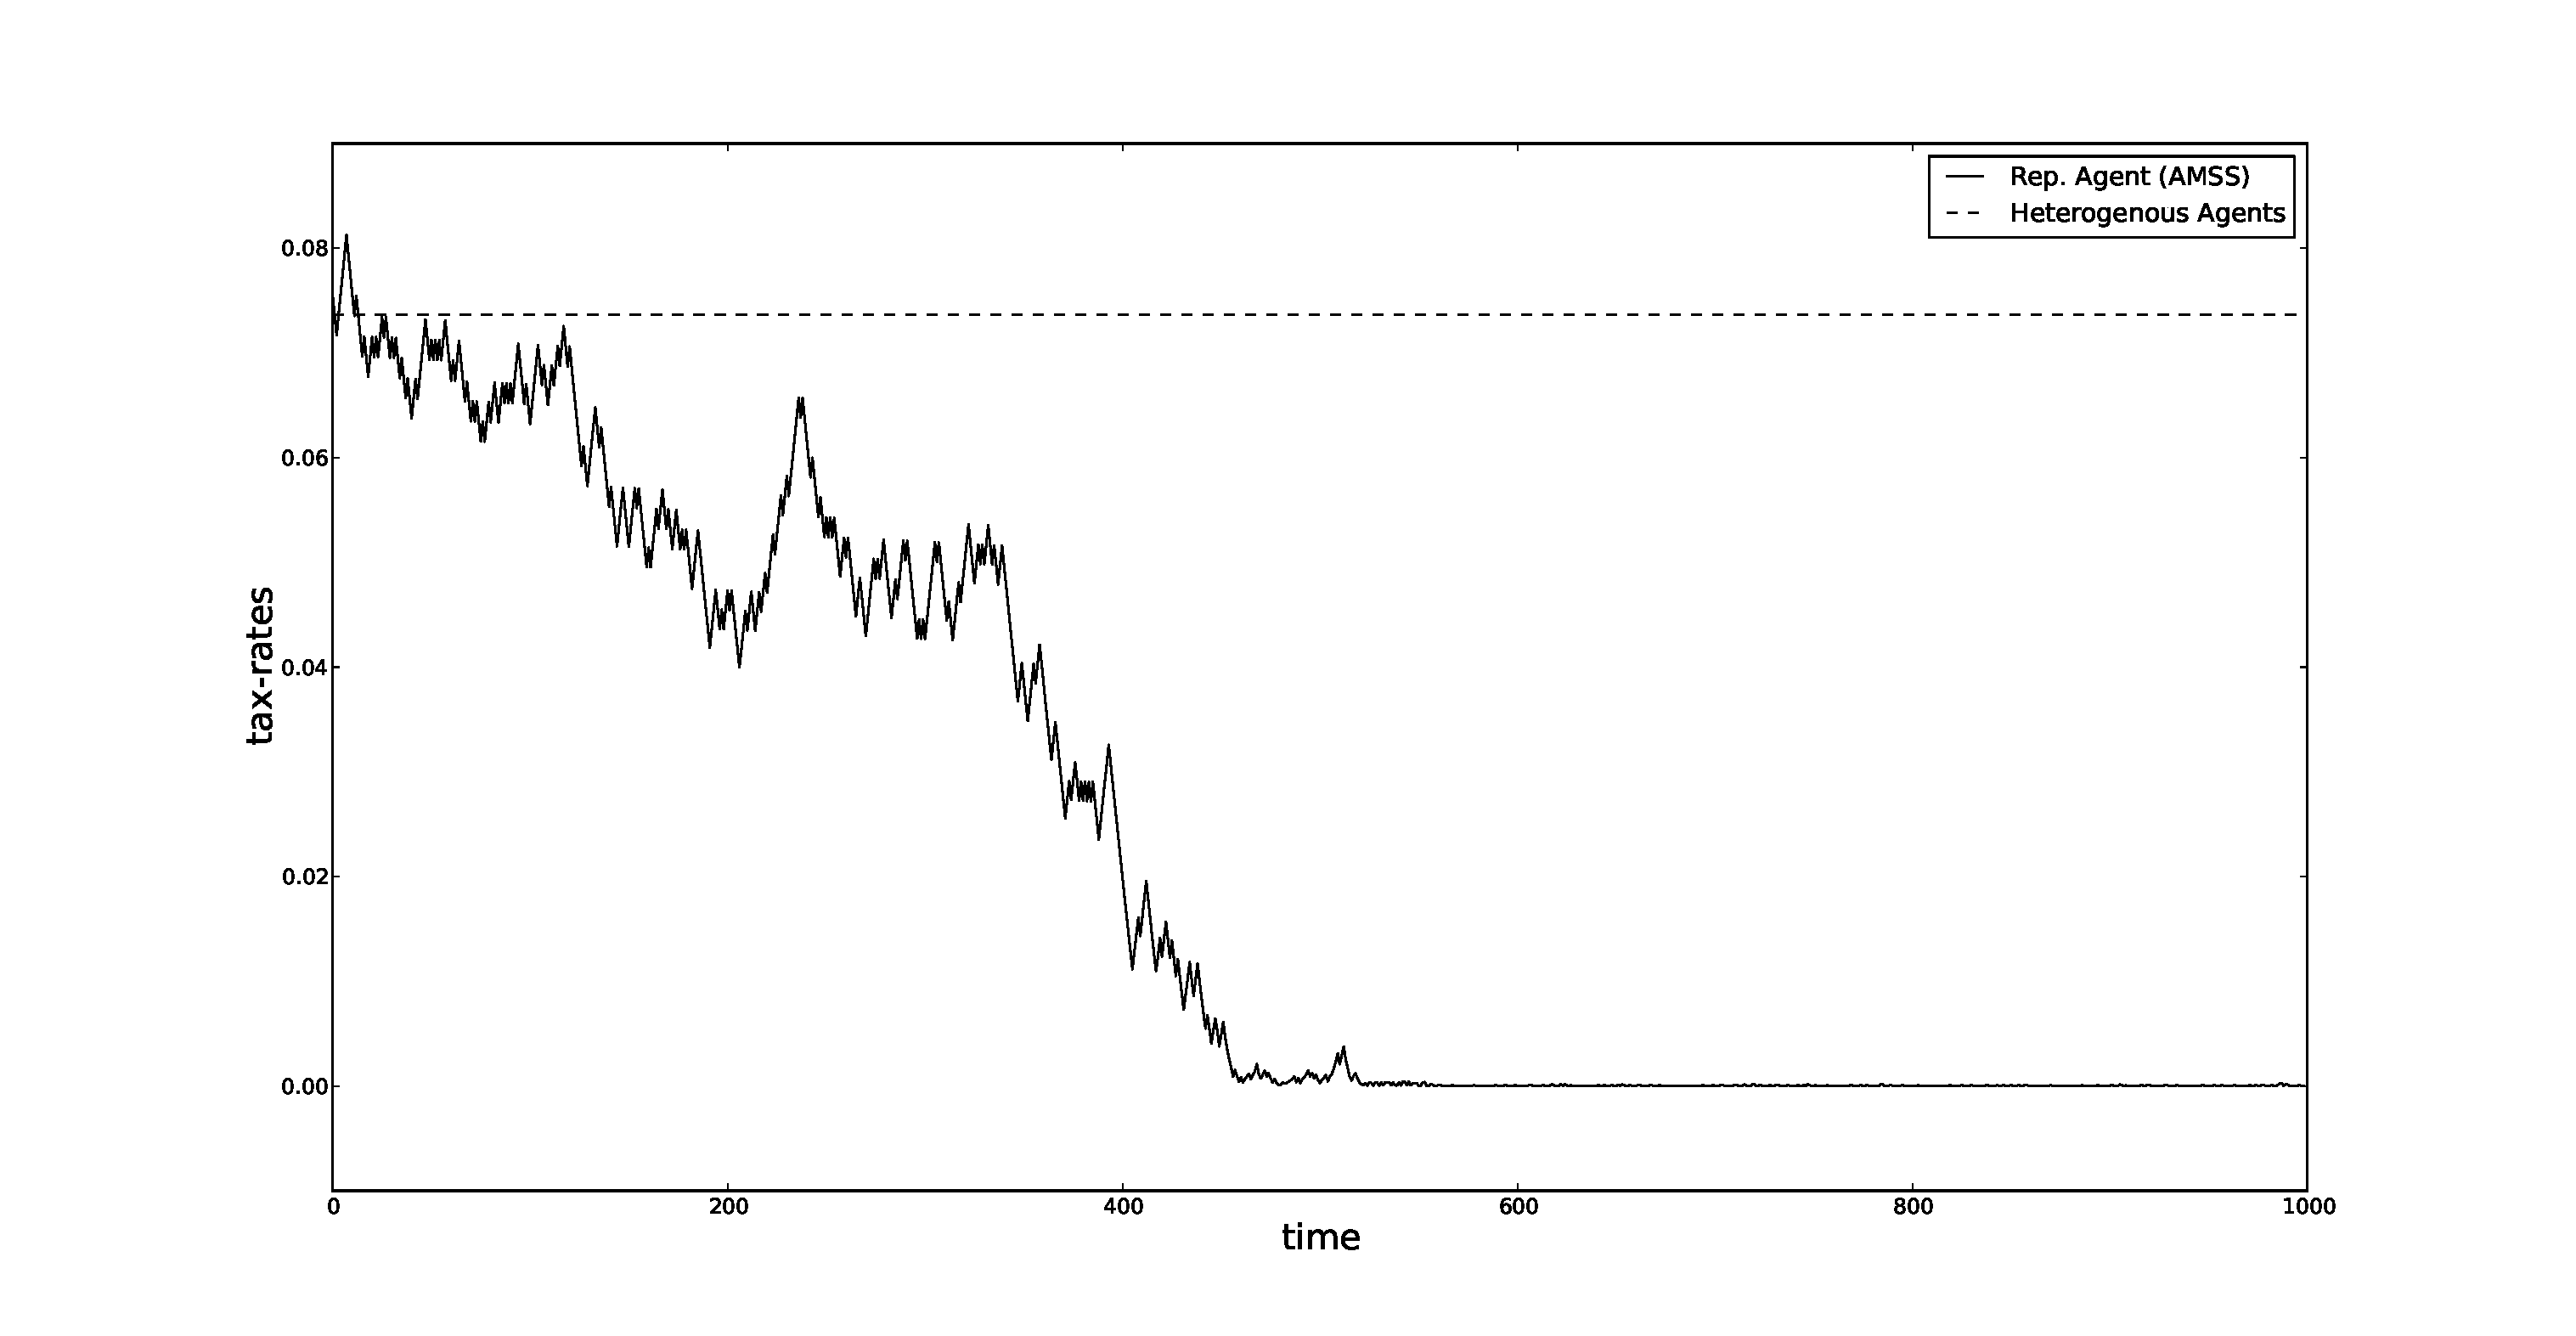
\includegraphics[width=\textwidth]{Draft25Graphs/BEGS_AMSS.eps}
 \caption{ Taxes in AMSS (solid line) and heterogeneous agent economy (dotted line) with quasi-linear preferences}
 \label{fig: AMSS vs BEGS}
 \end{figure}



\section{Optimal equilibria with affine taxes}\label{Sec: characterization}
%\textcolor{blue} {Remark from Anmol : I moved this section forward. This helps making the flow of the paper better. Once we setup the characterization  , the next two section deal with special cases where we prove theorems and the last section describes the numerical results}
%\textcolor{red}{Anmol -- I approve very much. I have done some editing.}

% This section prepares a recursive formulation of a Ramsey planner's problem with affine taxes in a risk-free-bond only economy. We  display
% implementability conditions and two  Bellman equations associated with the planning problem.
%  In section \ref{Sec: quasilinear}, we use these Bellman equations to characterize an optimal equilibrium in an economy with quasilinear preferences. In section \ref{sec: longrun anatyt},  we use them to study asymptotic outcomes under more general preferences.     In section \ref{Sec: numerical}, we use numerical solutions of these Bellman equations to study a calibrated economy.


 We return to our original problem formulated in section \ref{Sec: characterization}. We further assume assume that $U^{i}:\mathbb{R}%
_{+}^{2}\rightarrow \mathbb{R}$ is concave in $\left( c,-l\right) $ and
twice continuously differentiable. We let $U_{x,t}^{i}\ $or $U_{xy,t}^{i}$
denote first and second derivatives of $U^{i}$ with respect to $x,y\in
\left\{ c,l\right\} $ in period $t$ and assume that $\lim_{x\rightarrow \bar{%
l}_{i}}U_{l}^{i}\left( c,x\right) =\infty ,$ $\lim_{x\rightarrow
0}U_{l}^{i}\left( c,x\right) =0$ for all $c$ and $i.$

We focus on  interior equilibria. First-order necessary conditions for the  consumer's problem
 are%
\begin{equation}
\left( 1-\tau _{t}\right) \theta _{i,t}U_{c,t}^{i}=-U_{l,t}^{i}
\label{FOC consumption labor}
\end{equation}%
and%
\begin{equation}
U_{c,t}^{i}=\beta_tR_{t}\mathbb{E}_{t}U_{c,t+1}^{i}.  \label{FOC Euler}
\end{equation}%
To help characterize an equilibrium, we use

\begin{proposition}
\label{prop: affine eqm nec and suff}A sequence $\{ \left \{
c_{i,t},l_{i,t},b_{i,t}\right \} _{i},R_{t},\tau _{t},T_{t}\}_t$ is part of
a competitive equilibrium with affine taxes if and only if it satisfies (\ref%
{feasibility goods}), (\ref{agent bc affine}), (\ref{FOC consumption labor}%
), and (\ref{FOC Euler}) and $b_{i,t}$ is bounded for all $i$ and $t.$
\end{proposition}

\begin{proof}
Necessity is obvious. In the appendix \ref{appndx: affine eqm nec and stuff}, we use arguments of \cite{Magill1994} and \cite{Constantinides1996} to show that any $\left \{
c_{i,t},l_{i,t},b_{i,t}\right \} _{i,t}$ that satisfies (\ref{agent bc
affine}), (\ref{FOC consumption labor}), and (\ref{FOC Euler}) is a solution
to consumer $i$'s  problem. Equilibrium $\{B_{t}\}$ is determined by
(\ref{feasibility bonds}) and constraint (\ref{govmt bc affine}) is then
implied by Walras' Law
\end{proof}

To find an optimal equilibrium, by Proposition  \ref{prop: affine eqm nec and suff}
we can choose $\{ \left \{ c_{i,t},l_{i,t},b_{i,t}\right \} _{i},R_{t},\tau
_{t},T_{t}\}_{t}$ to maximize (\ref{govmt objective}) subject to (\ref{feasibility goods}), (\ref{agent bc affine}),(\ref{FOC consumption labor}), and (\ref{FOC Euler}).
% The last two constraints determine $\left \{ R_{t},\tau _{t}\right \}
%_{t} $ and are not featured anywhere else in maximization, so the
%allocations can be optimized over $\{\left \{
%c_{i,t},l_{i,t},b_{i,t}\right \} _{i},,T_{t}\}_t$ which often simplifies
%optimization.
We  apply a first-order approach and follow steps similar to ones taken by \cite{LucasJr.1983} and AMSS.
 Substituting consumers' first-order
conditions (\ref{FOC consumption labor})\ and (\ref{FOC Euler})\ into the
budget constraints (\ref{agent bc affine}) yields implementability
constraints%
\begin{equation}
c_{i,t}+b_{i,t}=-\frac{U_{l,t}^{i}}{U_{c,t}^{i}}l_{i,t}+T_{t}+\frac{%
U_{c,t-1}^{i}}{\beta_{t-1} \mathbb{E}_{t-1}U_{c,t}^{i}}b_{i,t-1}\ \text{for\ all\ }%
i,t.  \label{affine implementability a}
\end{equation}

\noindent For $I\geq 2$, we can use constraint (\ref{affine implementability
a}) for  $i=1$ to eliminate $T_{t}$ from (\ref{affine implementability a}) for $i > 1$. Define $\tilde{b}%
_{i,t}\equiv b_{i,t}-b_{1,t}$ we can represent the implementability constraints
as
\begin{eqnarray}
&&\left( c_{i,t}-c_{1,t}\right) +\tilde{b}_{i,t}
\label{affine implementability b} \\
&=&-\frac{U_{l,t}^{i}}{U_{c,t}^{i}}_{i,t}l_{i,t}+\frac{U^1_{l,t}}{U^1_{c,t}}l_{1,t} +\frac{U_{c,t-1}^{i}}{\beta_{t-1} \mathbb{E}%
_{t-1}U_{c,t}^{i}}\tilde{b}_{i,t-1}\ \text{for\ all\ }i>1,t.  \notag
\end{eqnarray}
\noindent With this representation of the implementability constraints, the planner's
maximization problem depends only on the $I-1$ variables $\tilde{b}_{i,t-1}.$
The reduction of  the dimensionality from \ $I$ to $I-1$ is
 another consequence of theorem \ref{theorem: main}.

 We can now write the problem recursively. Let $\bm{x}= \beta^{-1}\left( U_{c}^{2}\tilde{b}_{2},...,U_{c}^{I}\tilde{b}_{I}\right)$, $\bm{\rho }=\left( U_{c}^{2}/U_{c}^{1},...,U_{c}^{I}/U_{c}^{1}\right) $, and denote an allocation $a=\{c_i,l_i\}^{I}_{i=1}.$
In the spirit of \cite{Kydland1980} and \cite{Farhi2010}, we split the problem into a time-0 problem that takes $(\{\tilde{b}_{i,-1}\}^{I}_{i=2}, s_0)$ as given and   a time $t \geq 1$ continuation problem  that takes $\bm x,\bm \rho,s\_$ as given. We formulate
two Bellman equations and two value functions, one that pertains to $t\geq 1$, another for $t=0$.

\smallskip
%\textcolor{blue}{Anmol: I have changed both the Bellman equations to incorporate $\beta$ shocks inline of David's suggestion}
For $t\geq1$, let $V(\bm{x},\bm{\rho },s\_)$ be the continuation value to the planner given $\bm x_{t-1}=\bm x,\bm \rho_{t-1}=\bm \rho,s_{t-1}=s\_$. It satisfies the Bellman equation
%\textcolor{green}{David:  It seems to me that given that this is the Bellman equation we expect readers to refer to throughout the paper it might be good to allow for the possibility of discount factor shocks.  In which case the implementability should be
%\[
%	U_{c}^{i}\left[ c_{i}-c_{1}\right] +\beta x_{i}^{\prime }+\left( {U_{l}^{i}}%
%l_{i}-U_{c}^{i}\frac{U_{l}^{1}}{U_{c}^{1}}l_{1}\right) =\frac{xU_{c}^{i}}{%
% \mathbb{E}_{s\_}U_{c}^{i}}
%\] }
%\textcolor{red}{XXXXX I concur with David's suggestion. It might be good to add a sentence or remark emphasizing the $\beta$ depends on $s_{-}$.
%Also, a similar change is called for in the time $0$ Bellman equation isn't it?}
\smallskip\
\begin{equation}
V(\bm{x},\bm{\rho },s\_)=\max_{a(s),x^{\prime}(s),\rho^{\prime}(s)}{\sum_{s}\Pr {(s|s\_)\left( \left[
\sum_{i}{\pi _{i}\alpha _{i}U^{i}(s)}\right] +\beta(s) V(\bm{x}^{\prime
}(s),\bm{\rho }^{\prime }(s),s)\right) }}  \label{eq:BM2}
\end{equation}%
subject to  \label{eq:BM2_cons}
\begin{subequations}
\begin{equation}
U_{c}^{i}(s)\left[ c_{i}(s)-c_{1}(s)\right] +\beta(s) x_{i}^{\prime }(s)+\left( {U_{l}^{i}(s)}%
l_{i}(s)-U_{c}^{i}(s)\frac{U_{l}^{1}(s)}{U_{c}^{1}(s)}l_{1}(s)\right) =\frac{xU_{c}^{i}(s)}{%
 \mathbb{E}_{s\_}\bm{U}_{c}^{i}}\text{ for all }s,i\geq 2  \label{eq:BM2_Imp_cons}
\end{equation}%
\begin{equation}
\frac{\mathbb{E}_{s\_}\bm{U}_{c}^{i}}{\mathbb{E}_{s\_}\bm{U}_{c}^{1}}%
=\rho _{i}  \text{ for all }i\geq 2 \label{eq:BM2_Bonds_cons}
\end{equation}%
\begin{equation}
\frac{U_{l}^{i}(s)}{\theta _{i}(s)U_{c}^{i}(s)}=\frac{U_{l}^{1}(s)}{\theta
_{1}(s)U_{c}^{1}(s)}\text{ for all }s,i\geq 2  \label{eq:BM2_Wages_cons}
\end{equation}%
\begin{equation}
\sum_{i}\pi _{i}c_{i}(s)+g(s)=\sum_{i}\pi _{i}\theta _{i}(s)l_{i}(s)  \ \ \forall s
\label{eq:BM2_Res_cons}
\end{equation}%
\begin{equation}
\rho _{i}^{\prime }(s)=\frac{U_{c}^{i}(s)}{U_{c}^{1}(s)} \text{ for all } s,i\geq 2 \label{eq:BM2_rhoprime}
\end{equation}
\end{subequations}
Constraints (\ref{eq:BM2_Bonds_cons}) and (\ref{eq:BM2_rhoprime}) implies (\ref{FOC Euler}). The definition of $x_t$ and  constraints (\ref{eq:BM2_Imp_cons}) together exhausts equation (\ref{affine implementability b}) scaled by $U^i_c$. 

%Period 0 maximization problem is the similar except constraint (\ref{eq:BM2_Bonds_cons}) is absent and we normalize the initial debt to be inclusive of accrued interest.
Let $V_0\left(\{\tilde{b}_{i,-1}\}^{I}_{i=2},s_0\right)$ be the value to the planner at $t=0$, where $\tilde b_{i,-1}$ denotes initial debt inclusive
of accrued interest.   It satisfies the Bellman equation
\begin{equation}
V_0\left(\{\tilde{b}_{i,-1}\}^{I}_{i=2}, s_0\right) = \max_{a_0,x_0,\rho_0} {\sum_{i}\pi_i\alpha_i U^i(c_{i,0},l_{i,0}) + \beta(s_0) V\left(x_0,\rho_0,s_0\right)
}
\end{equation}
subject to
%\textcolor{red}{XXXXX Should  a similar change to the one David recommended be executed here?}
\begin{subequations}

\begin{equation}
U_{c,0}^{i}\left[ c_{i,0}-c_{1,0}\right] +\beta (s_0)x_{i,0}+\left( {U_{l,0}^{i}} l_{i,0}-U_{c,0}^{i}\frac{U_{l,0}^{1}}{U_{c,0}^{1}}l_{1,0}\right) = U_{c,0}^{i}\tilde{b}_{i,-1} \text{ for all } i\geq 2
\end{equation}

\begin{equation}
\frac{U_{l,0}^{i}}{\theta _{i,0}U_{c,0}^{i}}=\frac{U_{l,0}^{1}}{\theta
_{1,0}U_{c}^{1,0}}\text{ for all } i\geq 2
\end{equation}
\begin{equation}
\sum_{i}{\pi_{i}c_{i,0}}+g_0=\sum_{i}{\pi_{i}\theta_{i,0}l_{i,0} }
\end{equation}
\begin{equation}
\rho _{i,0}=\frac{U_{c,0}^{i}}{U_{c,0}^{1}} \text{ for all } i\geq 2
\end{equation}
\end{subequations}

The time $0$ problem  differs from the time $t \geq 1$ problem  since constraint (\ref{eq:BM2_Bonds_cons}) is absent from the
time $0$ problem.



\section{Ergodic distribution and policies in the long run } \label{sec: SteadyStates}
In this section, we characterize the properties of the ergodic set to which state variables converge over time. We start with a case when aggregate shocks are iid and can take two values. We show that for this shock structure there generally exists a ``steady state'' $\left( \bm{x}^{SS},\bm{\rho} ^{SS}\right) $  such that if economy ever reaches this state, it stays there.  Taxes and transfers in this steady state depend only on the current realization of the shock and the fluctuations of taxes is small for commonly used preferences. We also characterize properties of the steady state, discuss conditions under which economy converges to it and the speed of convergence.   Section \ref{Sec: More General Shocks}  then extends the analysis to more general shocks and shows numerically that while the ``steady state'' generally does not exist, the properties of the ergodic set are very similar to those in the two shock iid case. Throughout this section we assume that preferences are separable in consumption and 
labor.
% 
% 
% we first use the Bellman equations of section \ref{Sec: Bellman Equations} to study a class of economies where shocks are binary (i.e take two values) and IID over time. This restriction allows us to characterize ``steady states'' of the $t\geq1$ recursive problem described in (\ref{eq:BM2}). These are values of state variables $(\bm{x},\bm{\rho})$ such that associated optimal policies from this node are stationary. After setting up necessary conditions for the existence steady state, we analyze an example with two agents to further study its working  and illustrate comparative statics. Section \ref{Sec: More General Shocks} and \ref{Sec: numerical} discus extensions to more general shock structures
\subsection{IID shocks with two values}
Let $\Psi \left( s;\bm{x},\bm{\rho },s\_\right) $ be an optimal  law of motion for the state variables
for the $t\geq1$ recursive problem, i.e. $\Psi \left( s;\bm{x},%
\bm{\rho },s\_\right) =\left( x^{\prime }\left( s\right) ,\rho ^{\prime
}\left( s\right) \right) $ that solves (\ref{eq:BM2}) given state $\left(
\bm{x},\bm{\rho },s\_\right) .$ 
\begin{definition}
 A steady state is $\left( \bm{x}^{SS},\bm{\rho} ^{SS}\right) $ that satisfies $\left(\bm{ x}^{SS},\bm{\rho}
^{SS}\right) =\Psi \left( s;\bm{x}^{SS},\bm{\rho} ^{SS},s_{-}\right) $ for all $%
\,s,s\_.$ 
\end{definition}
Since in this steady state $\rho_i =U_{c}^{i}(s)/U_{c}^{1}(s)$ does
not depend on the realization of shock $s,$ the ratio of marginal utilities
of the two agents is constant. The continuation allocation depends only on  $s_{t}$ and not on the  history $s^{t-1}$.% These outcomes are reminiscent though not quite identical to those in a complete market economy (see Werning
%2007).\footnote{\textcolor{blue}{David, I have changed it a bit, do you think it reflects our understanding better. The earlier one sounded too cautionary}
%The steady state allocation is optimal for a \emph{modified} complete market problem where the Planner has to additionally adhere to a specific ratio of pairwise consumption (or ``market weights'' as in Werning(2007). However we note that typically, there does not exist an initial distribution of  assets  and list of Pareto weights for which the optimal allocation with complete markets will \emph{coincide} with the aforementioned stationary allocation with incomplete markets.}

We first begin by noting that the competitive equilibrium implicitly identifies an allocation $\{c_i(s),l_i(s)\}_{i}$ given a choice for $\{\tau(s), \bm{\rho}(s)\}$ using equations (\ref{eq:BM2_Wages_cons}), (\ref{eq:BM2_Res_cons}) and (\ref{eq:BM2_rhoprime}).  Let us denote $U(\tau,\bm{\rho},s)$ as the value for the planner from the implied allocation using Pareto weights $\{\alpha_i\}_i$ , 
\[U(\tau,\bm{\rho},s)=\sum_{i}\alpha_i U^i(s).\]

Let $I_i(s)=[1-\tau(s)]l_i(s)-c_i(s)$ be the disposable income of agent $i$ in state $s$, define $Z_i(\tau,\rho,s)$ as the utility adjusted spread in the disposable income relative to Agent 1 :
\[Z_i(\tau,\bm \rho,s)=U^i_c(s)\left\{I_1(s)-I_i(s)\right\}.\]
% 
% Note that $\sum_{i=2}^{N}Z_i(\tau,\bm  \rho,s)$ is the marginal utility adjusted  primary deficit using the implied allocation. 
% 
% 
% 
% %Next we define $Z(\tau,\rho,s)$ as the marginal utility adjusted primary deficit using the implied allocation. 
% \[Z(\tau, \bm \rho,s)=c_1^{-\sigma}(s)\left\{NT(s)+g-\tau(s)\sum_{i=1}^{N}\left[\theta_il_i(s)\right]\right\}\]
%  
% 
 The optimal policy  solves the following Bellman equation for $\bm{x}(s^{t-1})=\bm{x},\bm{\rho}(s^{t-1})=\bm{\rho}$
% 
 \begin{equation}
 \label{eq:ss-obj}
 	V(\bm x,\bm \rho) = \max_{\tau(s),\bm \rho'(s),\bm x'(s)}\sum_s P(s)\left[ U(\tau(s),\bm \rho'(s),s) + \beta(s) V(\bm x'(s),\bm \rho'(s))\right] 
 \end{equation}

 
 subject to the constraints
 \begin{equation}
 \label{eq:ss-imp}
 	Z_i(\tau(s),\bm \rho'(s),s) +\beta(s) x'_i(s) = \frac{x_i U^1_c(\tau(s),\bm \rho'(s),s)}{\mathbb{E} U^1_c(\tau,\rho)}\text{   for all  $s,i \geq 2$,}\\  
 \end{equation}
\begin{equation}
\label{eq:bondcondtion} 
 	\sum_s P(s)U^i_c(\tau(s),\bm \rho'(s),s)(\rho_i'(s)-\rho_i) = 0 \text{  for $i \geq 2.$} 
\end{equation}
 
 Constraint (\ref{eq:bondcondtion}) is obtained by rearranging constraint (\ref{eq:BM2_Bonds_cons}). It implies that $\rho(s)$ is a risk-adjusted martingale and we use this property later to discuss convergence. We next check if the first order necessary conditions are consistent with stationary policies for some ($\bm x, \bm \rho$) \footnote{Appendix \ref{apndx: numerical methods} discuses the associated second order conditions that ensure these policies are optimal}. 
 \begin{lemma}\label{lemma-simplified-foc}
Let $P(s)\mu_i(s)$ and $\lambda_i$ be the multipliers on constraints ( \ref{eq:ss-imp}) and (\ref{eq:bondcondtion}).  Imposing the restrictions $x'_i(s) = x_i$ and $\rho'_i(s) = \rho_i$ the steady state solves for $\{\mu_i,\lambda_i,x_i,\rho_i\}^{N}_{i=2}$ and $\{\tau(s)\}_s$ using the following equations


\begin{subequations}
\label{sys-steadystate}
\begin{equation}
\label{eq:ss.imp.simplified}
  	Z_i(\tau(s),\bm \rho,s) +\beta(s) x'_i = \frac{x_i U^1_c(\tau(s),\bm \rho,s)}{\mathbb{E} U^1_c(\tau,\rho)}\text{   for all  $s,i \geq 2$,}\\  
\end{equation}
 \begin{equation}
	U_{\tau}(\tau(s),\bm \rho,s)-\sum_i\mu_i Z_{i,\tau}(\tau(s),\bm \rho,s)  =0 \text{  for all $s$,} \label{eq:foc.tau.simplified}\\
   \end{equation}
\begin{equation}
	U_{\rho_i}(\tau(s),\bm \rho,s) -\sum_j\mu_j(s)Z_{j,\rho_i}(\tau(s),\bm \rho,s)+ \lambda_iU^i_c(\tau(s),\bm \rho'(s),s)-\lambda_i\beta(s)\mathbb{E}U^i_c(\tau,\bm \rho) =0. \text{   for all $s,i \geq 2$ }\label{eq:foc.R.simplified}
 \end{equation}

\end{subequations}

\end{lemma}


Since the shock $s$ can take only two values, the system \eqref{sys-steadystate} is a square system in $4(N-1)+2$ unknows $\{\mu^{SS}_i,\lambda^{SS}_i,x^{SS}_i,\rho^{SS}_i\}^{N}_{i=2}$ and $\{\tau^{SS}(s)\}_{s}$. One can numerically verify that this system has a solution for wide range of primitives. In the next section we formally establish this for a class of simple two agent economies that, while special, illustrates general forces that affect outcomes. The example will help us  develop some comparative statics and interpret  outcomes from quantitative analysis in section \ref{Sec: numerical}.



Lemma \ref{lemma-simplified-foc} also highlights the tradeoffs that the planner faces.  Defining $\tilde{\lambda}=-\lambda \mathbb{E} U^i_c(\tau,\bm \rho)$ and taking expectations for equation (\ref{eq:foc.R.simplified}), we get that
\begin{equation}
\label{eq.ss.tradeoffs}
\mathbb{E} U_{\rho_i}(\tau(s),\bm \rho,s)= \mathbb{E} \sum_j\mu_j(s)Z_{j,\rho_i}(\tau(s),\bm \rho,s) + (1-\mathbb{E}\beta(s))\tilde{\lambda_i} 
\end{equation}
The multiplier on the implementability constraint for $i$ can be interpreted as the marginal costs of extracting funds from $i$  and $\tilde{\lambda_i}$ is proportional to the multiplier on the constraint $\frac{\mathbb{E}\bm{U}^i_c}{\mathbb{E}\bm{U}^1_c}=\rho$. This constraint ensures that at the optimal allocation, agent $i$ has no  incentives to participate in the risk free market to change his bond portfolios. The left hand side of \eqref{eq.ss.tradeoffs} captures the cost for the planner if inequality (measured by the ratios of marginal utilities of consumption) deviates from his ideal point, given by $\alpha_i/\alpha_1$. In the absence of any constraints, the planner would set $\mathbb{E} U_{\rho_i}(\tau(s),\bm \rho,s)=0$, which implies that $\alpha_i U^i_c = \alpha_1 U^1_c$ for all $i$. The right hand side of equation \eqref{eq.ss.tradeoffs} captures the costs of approching the planner's ideal point, which come from the costs of raising taxes (the first term on the left hand side) and ability of 
agents to trade with each other (the second term).

The behavior of the economy in the steady state is similar to the behavior of the complete market economy characterized by Werning (2007). Both taxes and transfers depend only on current relazation of shock $s_t$. Moreover, the arguments of Werning (2007) can be adapted directly to show that taxes are constant when preferences have a CES form $c^{1-\sigma}/(1-\sigma) - l^{1+\gamma}/(1-\gamma) $ and flucations in taxes is approximately zero when preferences take a balanced growth path form. We return to this point once we discuss convergence properties. 

\subsubsection{A two agent example}\label{sec: 2 agent example}

\smallskip Consider an economy consisting of  two types of households with $%
\theta _{1,t}>\theta _{2,t}=0$. One period utilities are $\ln c-\frac{1}{2}%
l^{2}.$ The shock $s$  takes  two values, $s\in \left\{
s_{L},s_{H}\right\} $ with probabilities $\Pr \left( s|s\_\right) $ that are
independent of $s_{-}.$ We assume that $g\left( s\right) =g$ for all $s,$
and $\theta _{1}\left( s_{H}\right) >\theta _{1}\left( s_{L}\right) .$ We allow the discount factor $\beta $ to depend on  $s.$

\smallskip

\begin{proposition}
\label{prop: long run forces}\smallskip Suppose that $g<\theta (s)$ for all $%
s.$

\begin{enumerate}
\item \textbf{Countercyclical interest rates.} If $\beta \left( s_{H}\right) =\beta \left( s_{L}\right)$, then
there exists a steady state $\left( x^{SS},\rho ^{SS}\right) $ such that $%
x^{SS}>0,\ R^{SS}\left( s_{H}\right) <R^{SS}\left( s_{L}\right) .$
\item \textbf{Acyclical interest rates.}  There exists a pair $\left\{ \beta \left( s_{H}\right) ,\beta \left( s_{L}\right)
\right\} $ such that there exists a steady state with $x^{SS}>0$ and $R^{SS}\left(
s_{H}\right) =R^{SS}\left( s_{L}\right)$.
\item \textbf{Procyclical interest rates.} There exists a pair  $\left\{ \beta \left( s_{H}\right) ,\beta \left( s_{L}\right)
\right\} $ such that there exists a steady state with $x^{SS}<0$ and  $R^{SS}\left( s_{H}\right) >R^{SS}\left( s_{L}\right) .$
\end{enumerate}
In all cases, taxes $\tau(s)=\tau^{SS}$ are independent of the realized state. 
\end{proposition}


In this two agent case, normalizing assets of the unproductive agent (using theorem \ref{theorem: main}) we can interpret $x$ as the marginal utility adjusted assets of the government. Besides establishing existence, the proposition identifies the importance of cyclical properties of real interest rates in determining the sign of these assets and thus enables us to compare our results to representative agent economies like AMSS.

Proposition \ref{prop: long run forces}  shows  two main forces that determine the dynamics of taxes
and assets: fluctuations in inequality and fluctuations in the interest rates. Let start with part 2 of proposition \ref{prop: long run forces}, which turns off the second force. When  interest rates are fixed, the government can adjust two
instruments in response  to an adverse  shock (i.e., a fall in $\theta_1$): it can either increase the  tax rate $%
\tau $ or it can decrease transfers $T.$ Both  responses are distortionary,
but for different reasons. Increasing the tax rate increases distortions because the deadweight loss is convex in the tax rate,
 as in \cite{Barro1979}. This force operates in our economy just as it does in  representative agent economies.
 But in a  heterogeneous agent economy like ours,  adjusting transfers $T$ is
also costly. When agents' asset holdings are identical, a decrease in transfers  disproportionately
affects a low-skilled agent, so his marginal utility
falls by more than does the marginal utility of a high-skilled agent. Consequently, a
decrease in transfers increases inequality, a cost  not present in  representative agent economies.

The government can reduce the costs of  inequality distortions by choosing
tax rate policies that make the net asset positions of  the high skilled agent
decrease over time. That makes the two agents'
after-tax and after-interest income  get closer
together, allowing decreases in transfers to have smaller effects on inequality in
marginal utilities. If the net asset position of a high skilled agent is
sufficiently low, then a change in transfers has no effect on inequality and
all  distortions from fluctuations in transfers are eliminated. \footnote{This convergence outcome has
 a similar flavor to "back-loading"\ results  of
 \cite{Ray2002} and \cite{Albanesi2012} that reflect the  optimality of structuring policies intertemporally eventually to disarm  distortions.}




% 
% If consumption is ordered i.e it is higher in booms than in recessions, interest rates are countercyclical. The government will hold positive assets as long as the steady state marginal utility adjusted primary deficit$Z(\tau,\rho,s)$ is countercyclical too.  

% It is possible to show numerically\footnote{Appendix \ref{apndx: numerical methods} describes a numerical test for existence and local stability cast in terms of  primitives.} that the steady state described in part
% 2 of  proposition \ref{prop: long run forces} is stable, so the  economy converges to it. This convergence outcome has
% a similar flavor to "back-loading"\ results  of
% \cite{Ray2002} and \cite{Albanesi2012} that reflect the  optimality of structuring policies intertemporally eventually to disarm  distortions.

% Theorem \ref{theorem: main} provides  a useful way to compare our results with
%  representative agent economies. By that theorem, we can normalize $%
% b_{2,t}=0 $ for all $t$, in which case the negative of net assets of high-skilled agents can be
% interpreted as assets of the government. Because $x^{SS}>0,$
% the government  accumulates assets over time$,$ as in  AMSS.

Turning now to the second force,  interest rates generally fluctuate
with  shocks.  Parts 1 and 3 of  proposition \ref{prop: long run forces} indicate what drives those  fluctuations. Consider again the example of a
decrease in productivity of high skilled agent. If the  tax rate  $\tau $ is left unchanged,
the government faces a shortfall of revenues. Since
$g$ is constant, the
government requires  extra sources of revenues. But  suppose that
the interest rate increases whenever $\theta_1 $ decreases, as happens, for
example, when  discount factors are
constant and $\theta_1 $ is the only source of shocks. If the government holds positive assets, its earnings from those assets increase.
 So holding assets allows higher interest income
 to offset some of the government's revenue losses from taxes on labor.  The situation reverses if interest rates fall at
times of increased need for government revenues, as in
 part 3 of  proposition \ref{prop: long run forces} and the steady state allocation features government holding debt.


 What matters for our second force is the comovement of the interest rate with fundamentals shocks. States with low average TFP (and therefore a lower base for labor taxes), high $g$, or a high spread of productivities that threatens to induce higher inequality (and therefore higher  transfers and thirst for more  government  revenues to finance them) are ``adverse'' from the point of view of current government finance. The government can cope with such adverse states in less distorting ways if finds itself holding positive (negative) assets if interest rates are  high (low). 

 %These are states in which, if there were no asset market and the government ran a balanced budget, the government would need to have a higher proportional tax rate in order to finance higher government expenditure, a lower tax base or transfers to counteract higher inequality.
 
Depending on  details of shock processes, these two forces can
either reinforce each other (as happens in Part 1 of  proposition \ref{prop: long run forces}) or work in the opposite direction (as in Part 3 of  proposition \ref{prop: long run forces}). In the latter case, whether the
government ends up with assets or debt in the long run depends on the
relative strengths of the two forces. 
 

 Besides discount factor shocks, the level of net assets in the steady state depends on other primitives too suchs as desire for redistribution. An interesting comparative static exercise is shutting off discount factor shocks and increasing  $\alpha_1$, the weight of the high-skilled agent. This implies that the planner taxes less the high skilled agent and redistributes less income to the low skilled agent. Since after-tax income of low skilled agent is lower, the fluctuation in transfers affects this agent more severe that the high skilled. To smooth this flucations the government needs to accumulate more claims on the high skilled, implying a positive relationship between the steady state level of government assets and Pareto weight on high skilled. Figure \ref{fig: SS comparative} plots how taxes and assets of the government vary as we change the Pareto weights on high type, $\alpha_1$.

 
 %As $\alpha_1 \to 1$, we approaches to a representative agent economy studied in AMSS.  Exploiting equation (\ref{eq:foc.tau.simplified}) to obtain a mapping between $\mu$ and $\tau$,  the steady state $(x^{SS},\rho^{SS})$ is  isomorphic to $(\tau^{SS},\rho^{SS})$.  In addition we also have that
% 
% \[	x=\frac{Z(\tau^{SS},\rho^{SS},s)}{\beta(R(s)-1)}\]
% 
% where \[Z(\tau, \bm \rho,s)=c_2^{-\sigma}(s)\left\{T(s)+g-\tau(s)\theta_1l_1(s)\right\}\]  is the marginal utility adjusted primary deficit in state $s$


  \begin{figure}[htp]
 \centering
 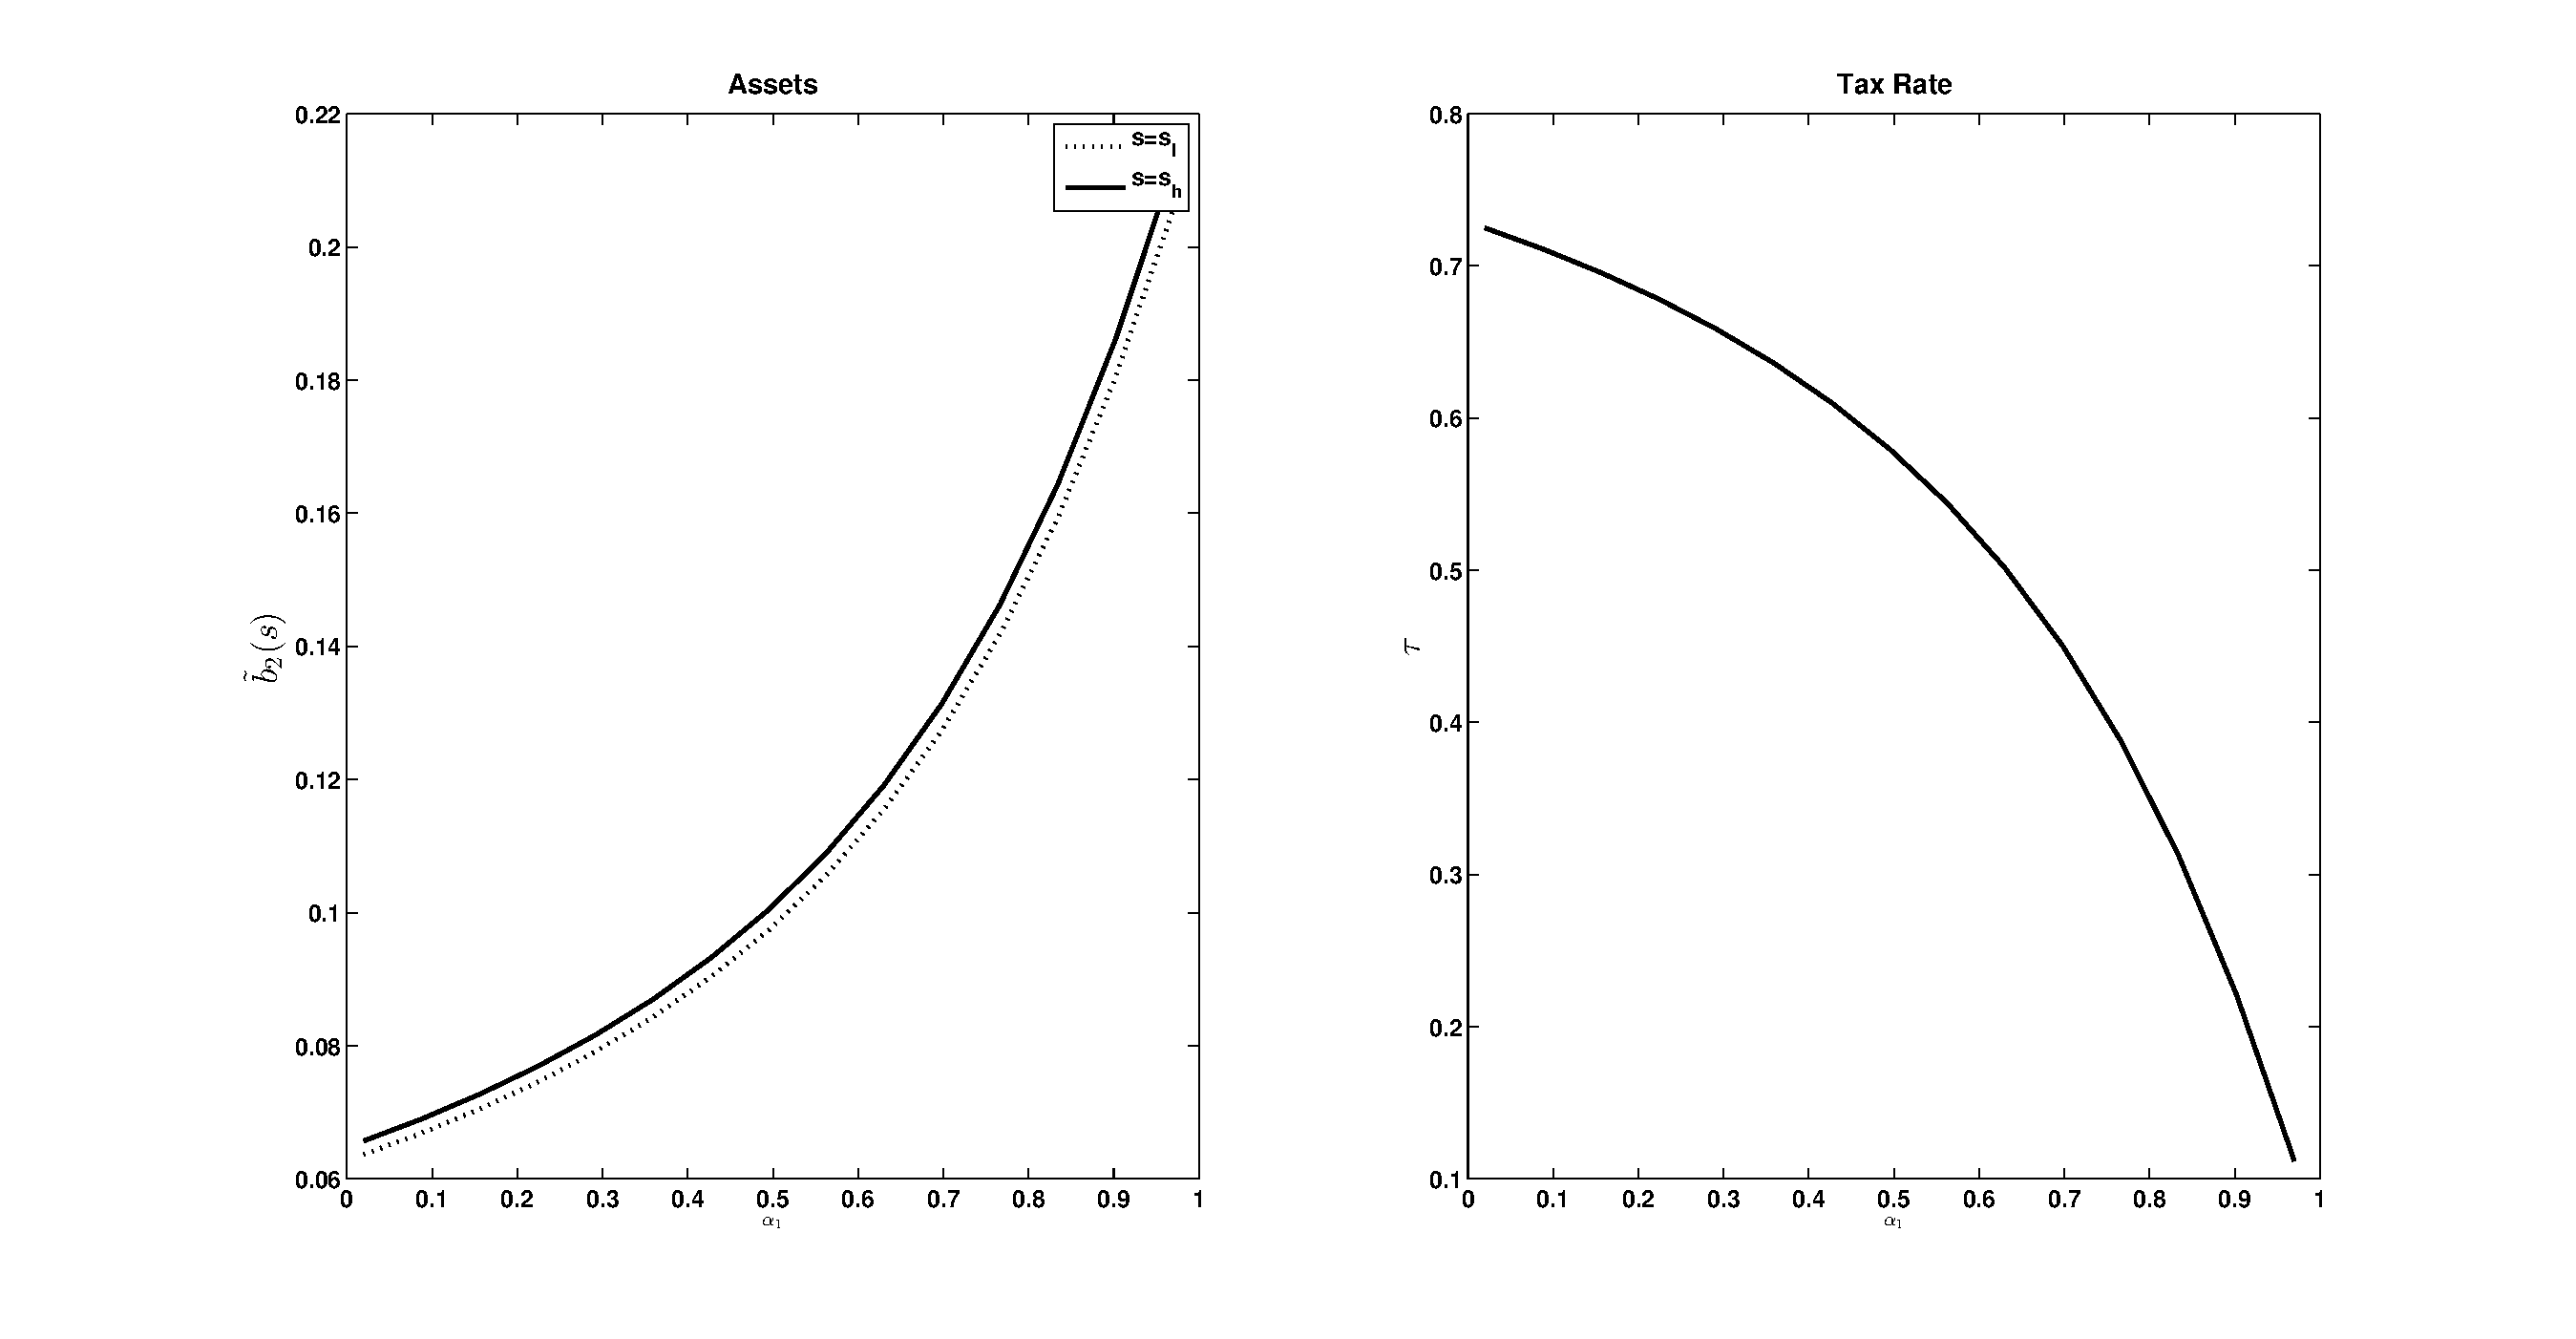
\includegraphics[width=\textwidth]{Draft25Graphs/SS_alpha1.eps}
 \caption{ Stead state assets : $\tilde{b}_2(s)=\frac{\beta  x^{SS}}{U^2_c(s)}$ and taxes : $\tau^{SS}$ as a function of Agent 1's (high skilled) Pareto weight}
 \label{fig: SS comparative}
 \end{figure}


Although we proved proposition \ref{prop: long run forces} for a particular
specification of preferences and shocks, the same  messages continue to hold more
generally.  The only place in the proof where we used the particular form of utility functions  was to prove an existence of a
solution to a particular equation that with our log-quadratic specification is  a quadratic that is
easy to solve analytically.  For other types of preferences, existence of a root for (\ref{sys-steadystate}) 
can be verified numerically. 

\subsection{Stability}
In this section we return to the general formulation of the problem from section \ref{Sec: characterization} to study convergence to the steady state. We first begin with testing for local convergence using a linear approximation of the policy rules at the steady state. Appendix \ref{apndx: numerical methods} describes a matrix equation, whose solution captures the coefficients of the linear approximation. 

Let $\hat{\Psi}_{t}= \left[\bmat x_{t} - x^{SS}\\ \rho_t - \rho^{SS}\emat\right]$ be the deviation from the steady state. The linear approximation solves for $B(s)$ such that
\begin{equation}
 \hat{\Psi}(s_{t+1},\hat{\Psi}_t)=B(s_{t+1})\hat{\Psi}_t \label{eq.linear.lom}
\end{equation}

\begin{proposition}\label{prop: localstability}
If the (real part) of eigenvalues of $\mathbb{E}B(s)$ are less than 1,  system (\ref{eq.linear.lom}) convergences to zero  in mean. Further for large $t$, the conditional variance of $\hat{\Psi}$ follows a deterministic process governed by 
\[\text{vec}(\Sigma_{\Psi,t})=\hat{B} \text{vec}(\Sigma_{\Psi,t-1})\]	
In addition,  if the (real part) of eigenvalues of $\hat{B}$ are less than 1, the system converges in distribution and probability.
\end{proposition}

The eigenvalues (in particular the dominant one) are instructive for (if and )how long it takes for the linearized system to converge. In figure \ref{fig: Eigenvalues} we return to the two agent example analyzed before and plot the eigenvalue of $\hat{B}$ that has the largest absolute value  and the associated half lives as a function of two primitives$\alpha_1$ and $\sigma$. It is clear that system is generically stable but the values close to 1 imply very slow convergence. In terms of 


The half-life is around 2800 years. We comeback to this feature in section \ref{Sec: numerical} where we study low frequency components of government debt.


  \begin{figure}[htp]
 \centering
 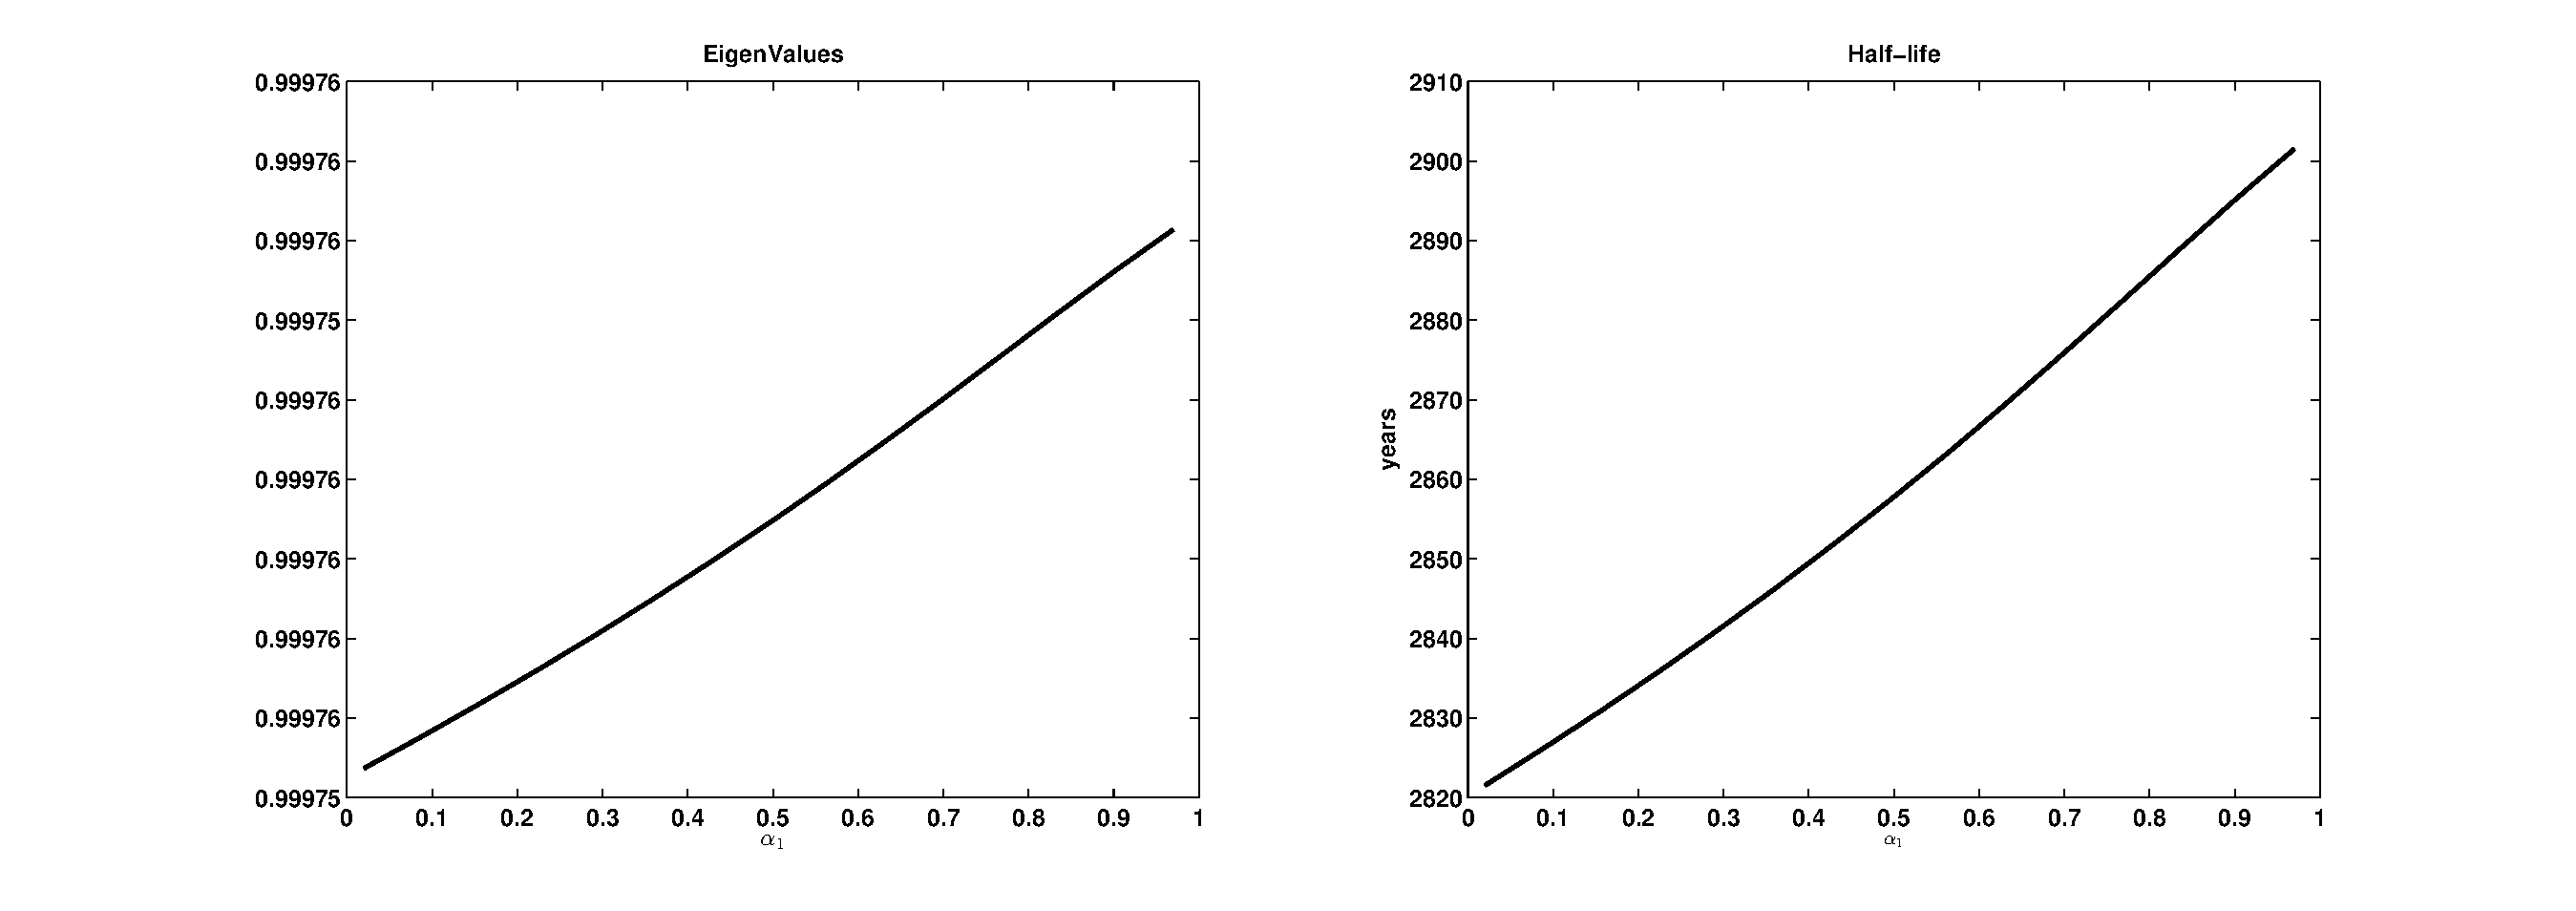
\includegraphics[width=\textwidth]{Draft25Graphs/eigenvalues_alpha1.eps}
 \caption{Eigenvalues of $\hat{B}$ (left panel) and associated half-life (right panel) as a function of Agent 1's (high skilled) Pareto weight}
 \label{fig: Eigenvalues}
 \end{figure}




Our first observation is that optimality conditions of problem (\ref{eq:BM2}) imply that the Language multiplier on the implementability constraint (\ref{eq:BM2_Imp_cons}) and the ratios of marginal utilities $\rho_{i,t}$ are risk-adjusted martingales. 

%A related set of questions besides existence of steady state are its stability properties. The optimal policy induces two risk adjusted martingales : $\mu_{t}$ %and $\rho_{t}$ where $\mu_{t}=V_{x}(\bm x_t,\bm {\rho}_t)$ \footnote{Such martingales often show up in related economies with implementability %constraints coming from market incompleteness, see for example AMSS }and $\rho_t=\frac{U^2_{c,t}}{U^1_{c,t}}$. 

The FOC for (\ref{eq:BM2}) with respect to $x(s)$ gives us% the $t \geq 1$, recursive problem $x'(s)$ gives us, 
\begin{align}
\mathbb{E} \frac{U^i_c(s)}{\mathbb{E}\bm{U}^i_c}\mu_i(s)=\mu_i\\
\mathbb{E} \mu_i(s)=\mu_i-cov\left[\mu_i(s),U^i_c(s)\right]
 \end{align}

 Similarly, rearranging the bond pricing equation \eqref{eq:BM2_Bonds_cons} implies
\begin{align}
\mathbb{E} \frac{U^1_c(s)}{\mathbb{E}\bm{U}^1_c}\rho_i(s)=\rho_i\\
\mathbb{E} \rho_i(s)=\rho_i-cov\left[\rho_i(s),U^1_c(s)\right]
 \end{align}

The first margingale shows up in the representative agent incomplete market models and captures that idea that the planner want to smooth fluctuations in distortions from taxes over time. The second martingale is new. It shows that fluctuations in inequality also follow a risk-adjusted martinage process.

\color{blue}{Anmol } WHAT DO WE NEED TO ARGUE THAT THERE IS A SUBMARTINGALE/SUPERMARTINGALE FORCES IN MU,RHO ? we need to show that if consumption is procyclical ,$\rho_i(s)$ and $\mu_i(s)$ are countercyclical  for a high enough $\mu_i,\rho_i$. Can this be simplified more ?


% As before, let  $I_i(s)=[1-\tau(s)]l_i(s)-c_i(s)$ be the disposable income of agent $i$ in state $s$. 
% 
% 
% \begin{proof}
% We need the following to argue that both process $\mu_t,\rho_t$ are sub-martingales  and bounded below by their steady state values. To show that they are submartingales we need to \textbf{sign the covariance} or with two shocks argue whether they are procyclical or countercyclical. The required bounds can be obtained by arguing that policy rules are \textbf{monotonic and continuous}. All of them are global poperties and have to hold uniformly in the relevant region. 
% I will elaborate the monotonicity requirement below.
% 
% Why should $\mu$ converge ? Suppose we assume
% \begin{itemize}
% \item $V(x,\rho)$ is concave in $x$ independently of $\rho$
% \item There exists a unique steady state 
%  \item $\beta(s)^{-1}U^2_c(s)\left[I_1(s)-I_2(s)\right]$ is countercyclical for all $\rho\geq\rho^{SS}$: \emph{The spread in disposable income is higher in
%  \item $c_i(s)$ is procyclical
%  recessions}
%  %\item $\rho(s)$ is countercyclical  : \emph{marginal utility of low skilled agent flucuates more than the high skilled agent}
% \end{itemize}
% 
% 
% \begin{enumerate}
%  \item First by assuming the value function is concave in $x$ all statements about $\mu$ can be translated to $x$ or assets.
%  \item $x'(x,\rho,s)$ is ordered for some $x\leq x^{SS}$ and $\rho\geq\rho^{SS}$
%   \textcolor{blue}{If we choose $x=0$, the implementability constraint implies that $x'(s)=-\beta(s)^{-1}U^2_c(s)\left[I_1(s)-I_2(s)\right]$. \footnote{If this property is true at the steady state we know that $x^{SS}>0$ as long as interest rates are countercyclical. This makes the choice of $x=0$ relevant} Thus requiring countercyclical spread in the disposable income gives us that $x'(s)$ is ordered at some point to the left of $x^{SS}$. Uniqueness of steady state ensures that this ordering at $x=0$ is uniform for all $x\leq x^{SS}$}
% 
%   \item $\frac{\partial x'(x,\rho,s)}{x}\geq0$ for all $x\leq x^{SS},\rho\geq\rho^{SS}$
%   
%   \textcolor{blue}{We can prove this if we sign $\mu^{SS}$. This is the argument : Suppose at the steady state the multiplier on the implementability constraint is positive. Concavity implies that it will be positive for all $x \leq x^{SS}$. Thus in this region having more assets or $x$ today  will slacken the constraint in both states tomorrow. This means that $\mu(x,\rho,s)$ will be lower and again through concavity $x'(x,\rho,s)$ will be higher}
%   \end{enumerate}
%   
% Together these porperties are sufficient to ensure that $\mu_t$ converges as long as consumption for agent 2 is procyclical
% 
% 
% Why should $\rho$ converge ? We again need to show similiar properties i.e
% 
% \begin{enumerate}
% \item We need $\rho(s)$ to be countercyclical for some node in the region $x\leq x^{SS}$ and $\rho\geq \rho^{SS}$. 
%  \item $\frac{\partial \rho'(x,\rho,s)}{\rho}\geq0$ for all $x\leq x^{SS},\rho\geq\rho^{SS}$
%   
%   \textcolor{red}{I am working on this}
%   
%   \item $\lim_{\rho\to \infty}\rho'(x,\rho,s)$ is ordered for all $x\leq x^{SS}$
%   
%   \textcolor{blue}{Ordering of $\rho(s)$ across states is same as ordering the following $\frac{U^i_c(s)-U^i_c(\tilde{s})}{U^i_c(\tilde{s})}$ across agents. Monotonicity implies that as $\rho$ goes to infity, $\rho(s)$ will go to infinity at least for some $s$. This means  $c_2(s)$ goes to zero. This makes $\frac{U^i_c(s)-U^i_c(\tilde{s})}{U^i_c(\tilde{s})}$  bounded for Agent 1 (as he consumes all the output) and goes to infinity or minus infinity for agent 2 as $c_2(s)$ goes to zero. Thus for large enough $\rho$,  $\rho'(s)$ is countercyclical. As with $x$, uniqueness of steady state means that this ordering is uniform for $\rho\geq \rho^{SS}$}
% \end{enumerate}
% 
% Together these porperties are sufficient to ensure that $\rho_t$ converges
% 
% 
% 
% 
% 
% \end{proof}
% 
% % 
% % Assumption 3  is sufficient for $x_{SS}>0$. Further at $x=0$ we have $x'(s)=-\beta(s)^{-1}U^2_c(s)\left[I_1(s)-I_2(s)\right]$. The countercyclical properties of the spread in disposable incomes yield that assets of the government are procyclical. Since having larger assets relaxes the implementability constraint, its multiplier $\mu(s)$ countercyclical. For high values of $\rho$, the unskilled agent has relatively low consumption and the fluctuations in ratio of marginal utilities is dominated by his marginal utilities. Thus $\rho(s)$ is countercyclical. Thus both covariances can be expected to be positive and $\rho_t,\mu_t$ are super martingales. The respective steady state values provide a lower bound and standard martingale convergence theorem would imply asymptotic converge
% 
% We realize that the previous argument depends on restrictions imposed on properties of endogenous objects like policy rules for consumption. However, they are intuitive from the trade-offs an optimal policy balances in such setting and are also confirmed in section \ref{Sec: numerical} where we study calibrated economies in more detail. It is nevertheless possible to get a more tighter test for local convergence using a linear approximation of the policy rules at the steady state. Appendix \ref{apndx: numerical methods} describes a matrix equation, whose solution captures the coefficients of the linear approximation.
% 
% Let $\hat{\Psi}_{t}= \left[\bmat x_{t} - x^{SS}\\ \rho_t - \rho^{SS}\emat\right]$ be the deviation from the steady state. The linear approximation solves for $B(s)$ such that
% \begin{equation}
%  \hat{\Psi}(s_{t+1},\hat{\Psi}_t)=B(s_{t+1})\hat{\Psi}_t \label{eq.linear.lom}
% \end{equation}
% 
% 
% 
% \begin{proposition}\label{prop: localstability}
% If the (real part) of eigenvalues of $\mathbb{E}B(s)$ are less than 1,  system (\ref{eq.linear.lom}) convergences to zero  in mean. Further for large $t$, the conditional variance of $\hat{\Psi}$ follows a deterministic process governed by 
% \[\text{vec}(\Sigma_{\Psi,t})=\hat{B} \text{vec}(\Sigma_{\Psi,t-1})\]	
% In addition,  if the (real part) of eigenvalues of $\hat{B}$ are less than 1, the system converges in distribution and probability.
% \end{proposition}
% 
% The eigenvalues (in particular the dominant one) are instructive for (if and )how long it takes for the linearized system to converge. In figure \ref{fig: Eigenvalues} we plot the eigenvalue of $\hat{B}$ that has the largest absolute value  and the associated half lives as a function of $\alpha_1$ for two agent economy analyzed before. It is clear that system is generically
% stable but the values close to 1 imply very slow convergence. The half-life is around 2800 years. We comeback to this feature in section \ref{Sec: numerical} where we study low frequency components of government debt.
% 
% 
%   \begin{figure}[htp]
%  \centering
%  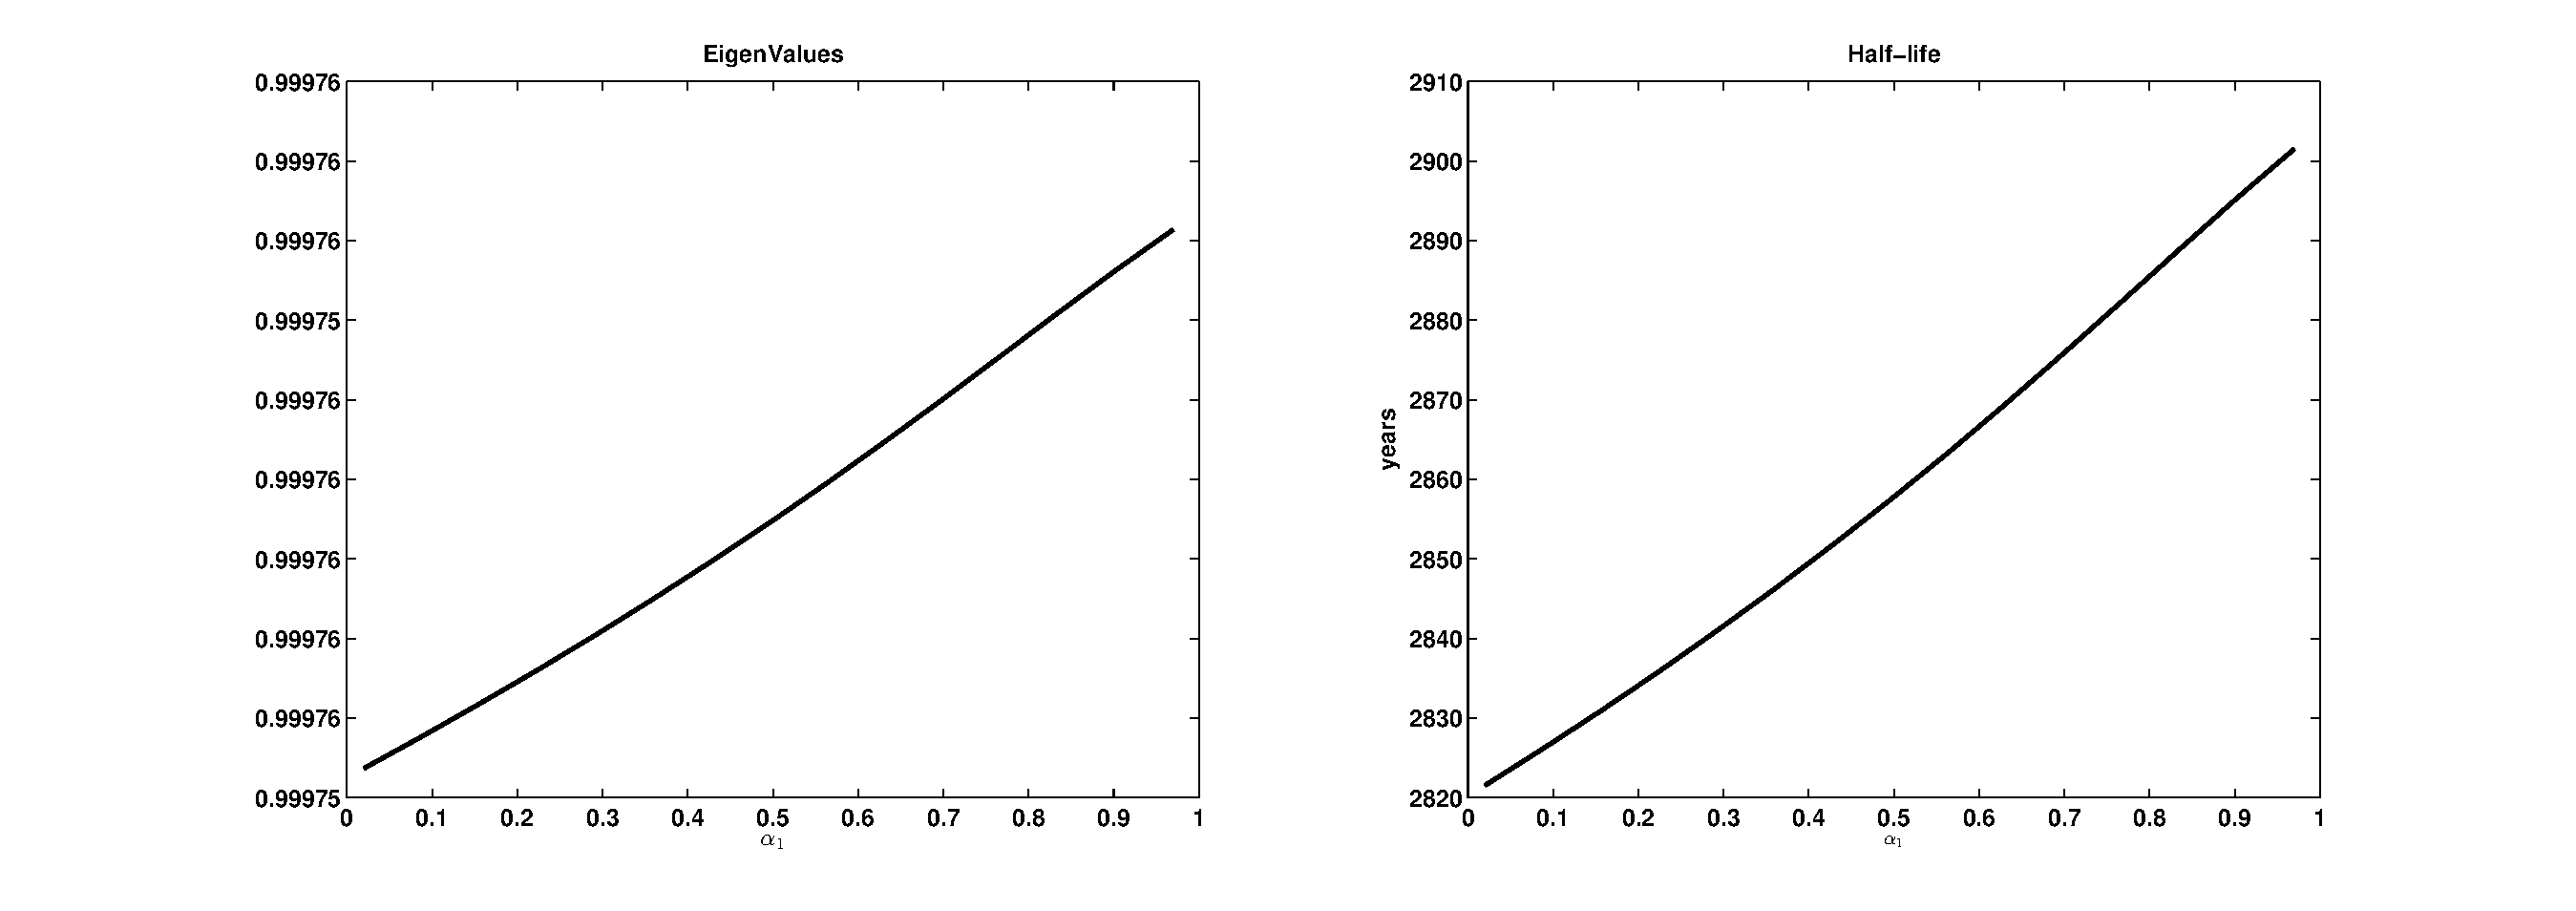
\includegraphics[width=\textwidth]{Draft25Graphs/eigenvalues_alpha1.eps}
%  \caption{Eigenvalues of $\hat{B}$ (left panel) and associated half-life (right panel) as a function of Agent 1's (high skilled) Pareto weight}
%  \label{fig: Eigenvalues}
%  \end{figure}
% 
% 
% 
\color{black}
\subsection{More general shocks} \label{Sec: More General Shocks}
The results on existence and convergence of steady state relied on a special binary-IID restriction. When there are more than two possible values for the shocks or when
shocks are persistent, the time-invariant steady state  will no longer
exist. Mathematically, this occurs because one asset and one risk-free rate
of return cannot span all possible needs for government revenues \footnote{One can see this from the fact that system \ref{eqs.ss} is no longer square}. With
richer shock structures, there exists an attraction region in the  $(x,\rho)$ space   to which the dynamic
system  converges. Although $\left( x,\rho \right) $ are no longer
constant in such region, their fluctuations tend to be markedly
reduced relative to the transients that occur away from that region, and general properties of $x$ and $\rho$ are the same as those
described in Proposition \ref{prop: long run forces}. Figure \ref{fig:moregeneralshocks} shows long sample paths for economies hit by more general TFP shocks. The top panel has IID shocks with 2 (bold) and 3(dotted) possible values and the bottom panel has persistent shocks with 2(bold) and 3 (dotted)possible values.
\textcolor{blue}{David, can you put a line explaining how the shock processes for this plot were calibrated}

% 
% 
   \begin{figure}[htp]
  \centering
  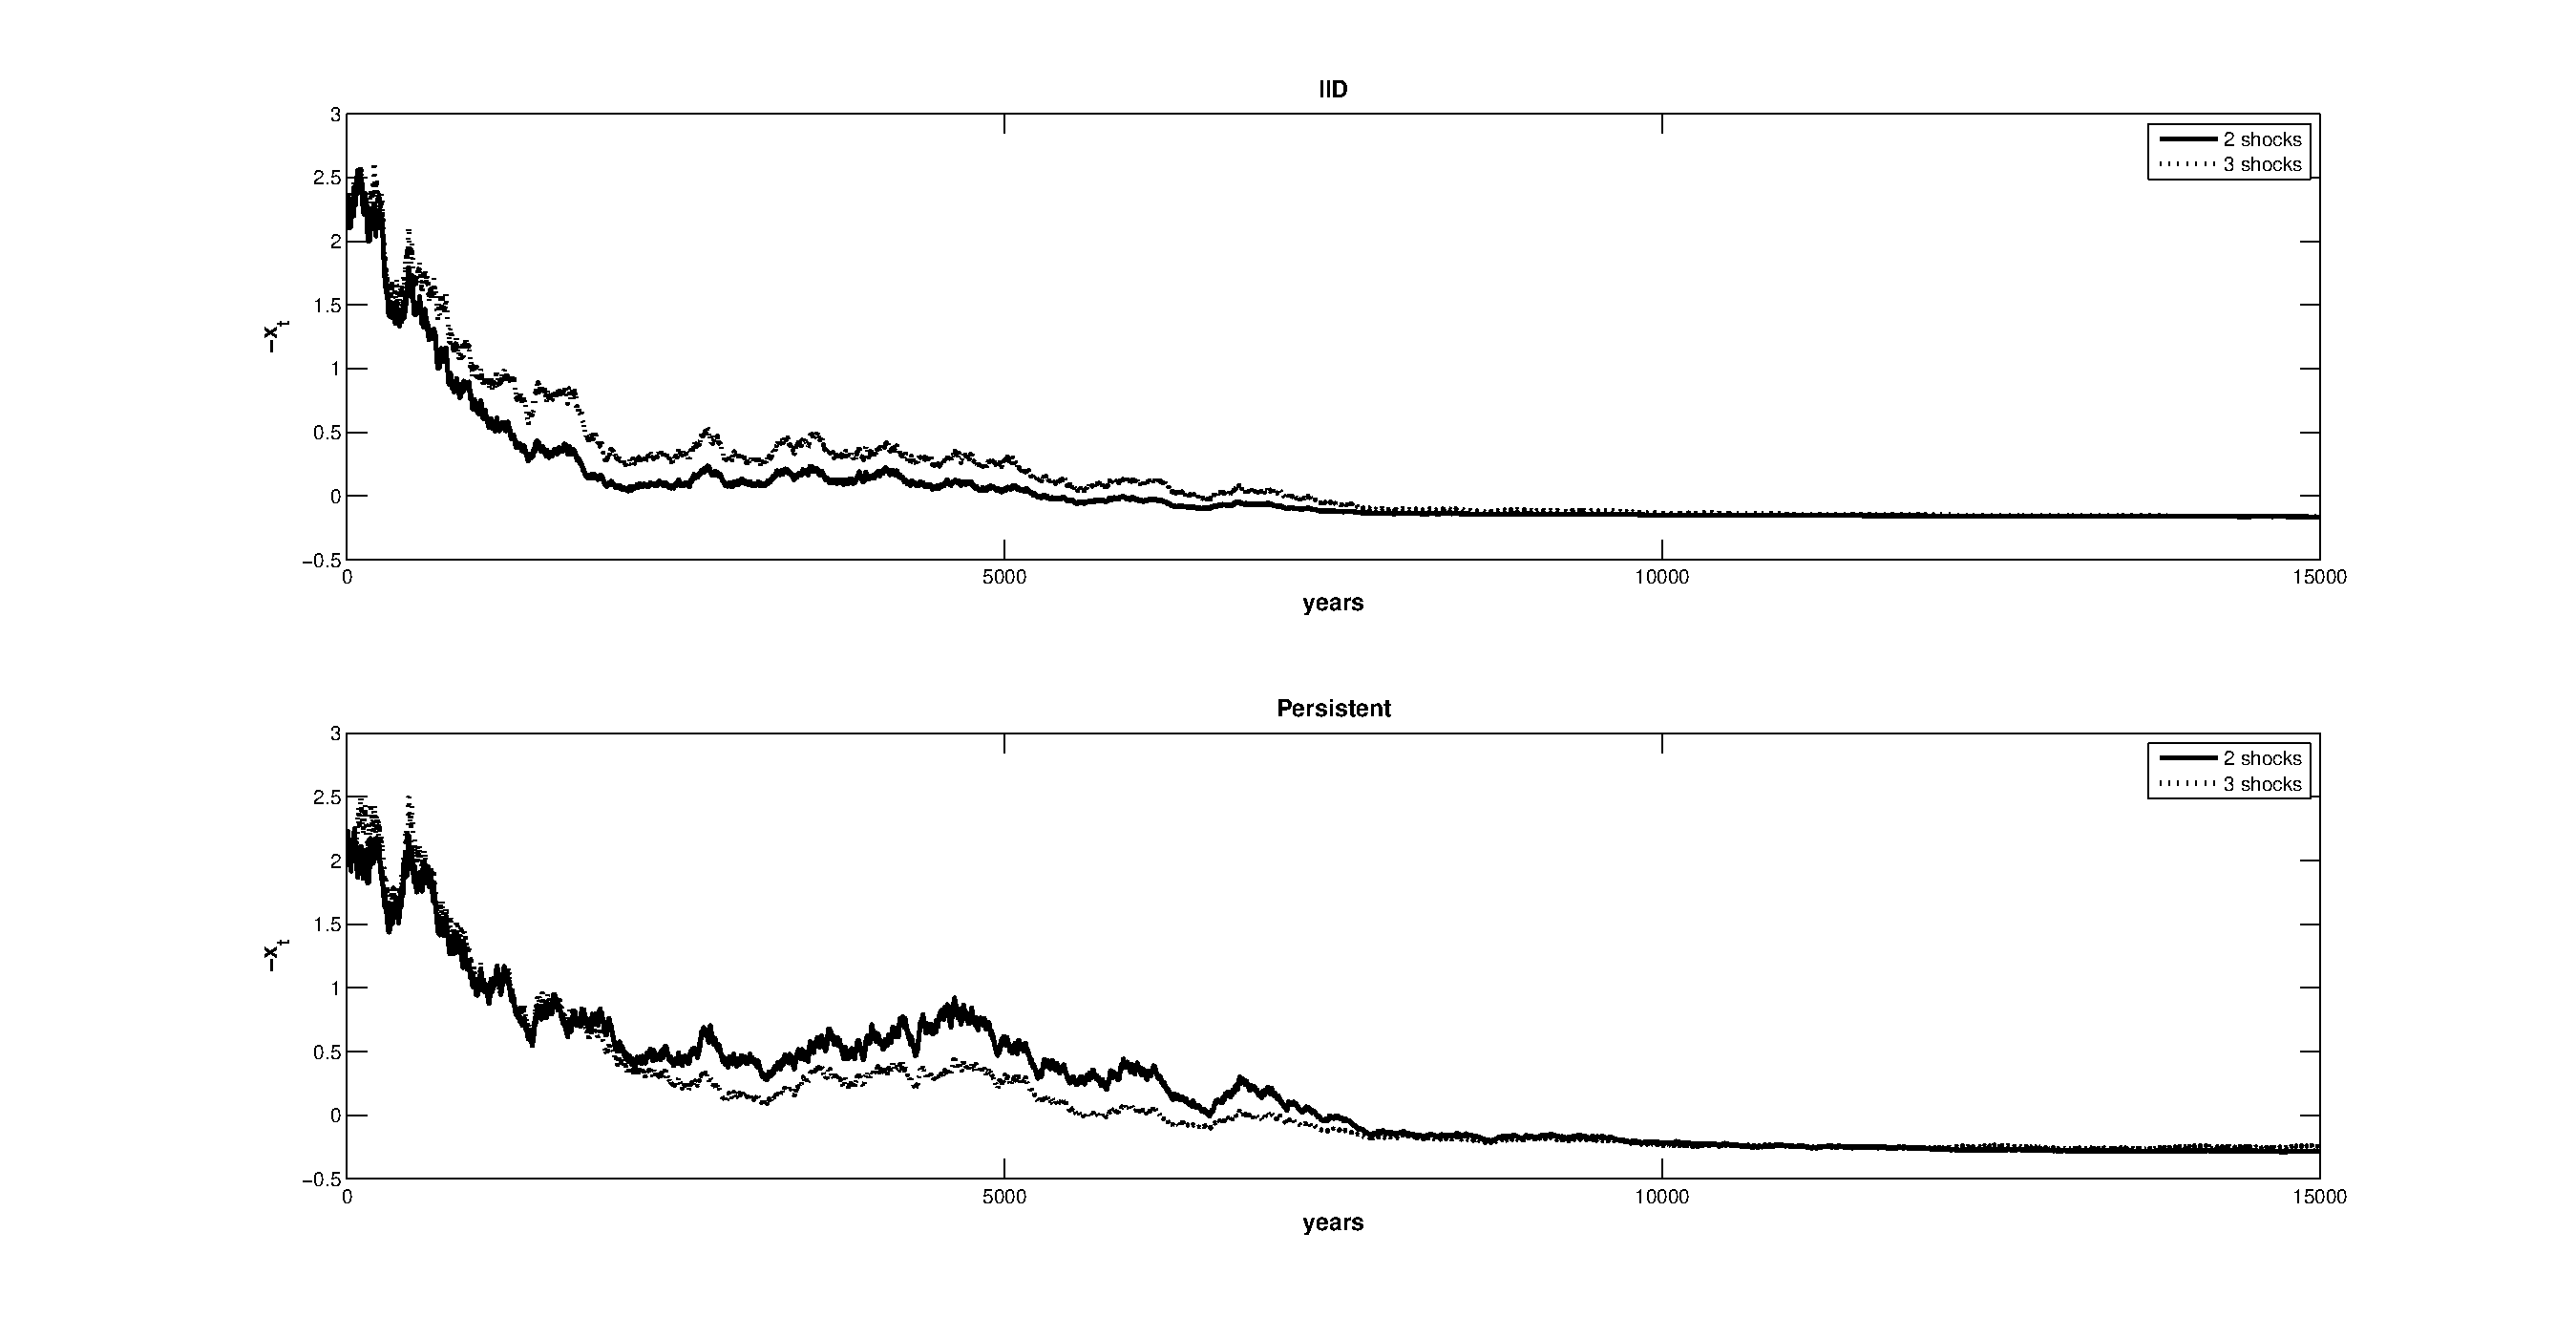
\includegraphics[width=\textwidth]{Draft25Graphs/generalshocks_x.eps}
  \caption{The figure depicts sample paths of marginal utility adjusted debt of the government i.e  $-x_t$. The top panel has IID shocks with 2 (bold) and 3(dotted) possible values and the bottom panel has persistent shocks with 2(bold) and 3 (dotted)possible values}
 \label{fig:moregeneralshocks}
  \end{figure}

\section{\protect\smallskip Optimal policy in booms and recessions}\label{Sec: numerical}

\smallskip

Section \ref{sec: 2 agent example} showed that the long run policy
response of the government depends on the nature of the shocks, in
particular, whether interest rates are high or low in periods which are ``adverse'' (low TFP, high inequality or high expenditure) from the point of view of governments budget constraint.

%on the correlation between the interest rate and the government's revenue
%requirements.
%\textcolor{red}{From Tom: Here the concept of `government's revenue
%requirements' makes an appearance. See my remark above. Let's clarify what it means.}
In this section, we further investigate this issue.
We focus on  optimal policy responses when the economy starts away
from the long-run steady state. We discuss  quantitative and qualitative
features of the response as well as the speed of convergence to the long-run
allocation by calibrating  shocks to match stylized facts about recent
recessions.

\smallskip We consider an economy with two types of agents%
of equal measures with preferences\footnote{%
We restrict our attention to the economy with two agents for computational
tractability. We want to understand both short-run and long-run
responses to shocks.  For some of our computations,  it is important to allow our
dynamic systems to travel over a large subset of state space, including regions encountered infrequently.
With more agents, it seems  possible to apply other methods,  for example those of  \cite{Judd2011}, to study dynamics of our economy within its invariant
distribution. We hope to pursue such extensions in  future work.}
\begin{equation*}
U\left( c,l\right) =\psi \ln c+\left( 1-\psi \right) \ln \left( 1-l\right) .
\end{equation*}%
The shock $s$   takes two values, $s_{H}$ and $s_{L}$, and follows a persistent
process. We allow $\beta ,$ $\theta _{i}$ and $g$ to be
functions of $s.$ We first pick $\bar{\theta}_{i},\bar{g}$
and $\bar{\beta}$ for a deterministic economy without shocks and calibrate $%
\left( \psi ,\alpha \right) $ to some low frequency  data moments. Then to match some business cycle moments we
pick shocks  according to
\begin{eqnarray}\label{eqn:newstar}
\theta _{i}(s) &=&\bar{\theta}_{i}[1+{\hat{\theta}}_{i}(s)], \cr
\beta \left( s\right) &=&\bar{\beta}\left[ 1+\hat{\beta}(s)\right] , \cr
g\left( s\right) &=&\bar{g}\left[ 1+\hat{g}\left( s\right) \right] ,
\end{eqnarray}%
where $\hat{\theta}_{i}\left( s\right) \in \{-e_{i,\theta },e_{i,\theta }\},$
$\hat{\beta}\left( s\right) \in \{-e_{\beta },e_{\beta }\}$ and $\hat{g}%
\left( s\right) \in \left\{ -e_{g},e_{g}\right\} .$ Throughout  our
experiments, we normalize $b_{2,t}=0$ for all $t\geq -1$. From market
clearing,  $B_{t}=-b_{1,t}$.  We refer to $B_{t}$ as
government debt (when negative) and  assets (when positive).

\smallskip

\subsection{\protect\smallskip Calibration}

\smallskip We calibrate the model in two steps. We first chose baseline parameters
that govern preferences and technology so  that an optimal equilibrium for the static%
\footnote{%
Formally, an equilibrium in an economy where all shocks are forever equal to their
mean value} version of the economy matches some sample moments in post war US data.  In the second step, we adjusted other parameters  to make the amplitudes of
fluctuations equal to average peak-trough spreads observed in
the  three most recent recessions (1991-92, 2001-02 and 2008-10).

\smallskip
We first discuss calibration of $\left( \psi ,\alpha ,\bar{\theta}%
_{i},\bar{g},\bar{\beta}\right) $. Although these parameters jointly
determine the relevant moments, it is helpful  to explain which moment
in the data mainly influences each parameter.   We normalize $\bar{\theta}_{2}=1$
and pick $\bar{\theta}_{1}$ to match log wage ratio of 90 wage percentile to
10 wage percentile of 4 from \cite{Autor2008}. We set the discount factor $\bar{\beta}$
 to match an (annual) interest rate of 2\%. We set the parameter $\psi $
to match Frisch elasticity of labor supply equal to $0.5$. In our model, $%
\bar{g}$ corresponds to non-transfer government expenditures, which
in the U.S. varied from 7\%  and  11\% in the post WWII period  and were above 20\% during the war. We set
 $\bar{g}$ to 12\% of GDP. Finally, we set Pareto weights $\alpha $ to match the average
marginal tax rate in the US\ of about 20\% as in \cite{Chari1994}. \footnote{We use federal government expenditures (excluding current transfers) since the labor tax rate of 20\% in  \cite{Chari1994} is calibrated to federal marginal taxes.}

\smallskip Next we turn to some business cycle targets. We calibrate $\left\{
e_{i,\theta },e_{\beta},\Pr \left( s|s_{-}\right) \right\} $ to match the
following four facts about booms and recessions (using NBER dates, for the last 3 recessions ie 1991-92, 2001-02 and 2008-10) : the log of the  incomes individuals at  both the 10th and the 90th percentile falls  the recessions; 10th percentile income falls by
more than 90th percentile; an  inflation-adjusted interest rate on government
debt is generally lower in recessions; and  booms last longer
than recessions. We calibrate the average spread in labor productivity  to
match the average 3\% loss in output seen in the last three recessions.%
\footnote{%
It has long been noticed that the standard RBC model predicts counterfactual
negative correlation between real interest rates and output (e.g. \cite{Boldrin2001}). In the data HP filtered output is roughly uncorrelated with real
interest rates, but this relationship turn positive if we look at peak vs
troughs. We report the optimal responses for both economies with positive
and zero correlation of interest rates and output and contrast with a
response to a pure TFP\ shock.} The inequality shock is designed to match
the facts documented in \cite{NBERw18035} that the fall in earnings of
the 10-percentile is about 2.5 times of 90-percentile.
 The discount factor shocks
match the average boom-recession difference of about 1.96\% in the real
risk-free interest rate (3 month T bill rate - inflation rate) seen in the
last three recessions. We calibrate the transition matrix  to get match the
average duration of booms vs recessions.
 For comparison, we also calibrate a drop in government expenditure to get a
drop in output  similar to recessions induced by the productivity shocks

Note that because each of them is an
exact function of $s_t$, government expenditures, the discount factor, and productivities are
perfectly correlated: a recession is an episode in which  TFP falls, inequality
rises, and the discount factor is  high. We set the initial level of government debt to be 60\%, roughly to match the ratio of federal debt held by public at the
beginning of 2010.

\smallskip  Table \ref%
{tab:Parameters} summarizes some  details about our calibration.

\smallskip

{\small
\begin{table}[htp]
{\small
\begin{tabular}{|l|c|c|c|}
\hline
Parameter & Target &  &  \\ \hline
$\psi$ & Frisch elasticity of labor supply & 0.6994 &  \\
$\bar{\theta}_1 $ & Log 90-10 wage ratio (Autor et all) & 4.0552 &  \\
$\bar{\theta}_2 $ & Normalize to 1 & 1 &  \\
$\hat {\theta}_1$ & Business cycle fluctuations in the earnings of 90th
percentile & 1.2 \% &  \\
$\hat{\theta}_2$ & Business cycle fluctuations in the earnings of 10th
percentile & 3\% &  \\
$\beta$ & Average (annual) risk free interest rate & 0.98 &  \\
$\hat{\beta}(s)$ & Business cycle fluctuations & .02 &  \\
$\alpha_1$ & marginal tax rate in the economy with no shocks & 0.69 &  \\
$g$ & average pre-transfer expenditure- output ratio & 12 \% &  \\
$P(r|r)$ & Recession-Boom episodes & 0.63 &  \\
$P(b|b)$ & Recession-Boom episodes & 0.84 &  \\ \hline
\end{tabular}
}
\caption{Benchmark calibration}
\label{tab:Parameters}
\end{table}
}

\subsection{Outcomes}

\smallskip

\smallskip We discuss separately  long run and  short run implications
for  optimal policy. In particular, we  study the economy (\textbf{%
``Benchmark''} ) with the calibration discussed above and a few variants
that successively turn off particular sources of variation.

\begin{enumerate}
\item \textbf{Acyclical Interest Rates}: In the first variant, we recalibrate
the discount factor shocks to make the risk-free rate be uncorrelated with
output.

\item \textbf{Countercyclical Interest Rates}: Here we shut off  discount
factor shocks by setting $\hat{\beta}\left( s\right) =0$ in \eqref{eqn:newstar}. Note that under
this assumption, interest rates are countercyclical.

\item \textbf{No Inequality}: This variant modifies the \textquotedblleft
Benchmark\textquotedblright\ by setting $\hat{\beta}\left( s\right) =0$ and $%
{\hat{\theta}}_{1}(s)={\hat{\theta}}_{2}(s)=3\%$ in \eqref{eqn:newstar}. This corresponds to a case
when the only source of business cycle fluctuations is a TFP shock that
affects all agents equally. This case more closely matches the experiments
in the RBC\ literature such as \cite{Chari1994}.

\item \textbf{Government expenditure Shocks}: The last variant compares  optimal
responses to shocks to government expenditures. In this experiment, we set
$\hat{\theta}\left( s\right) =\hat{\beta}\left( s\right) =0$ and choose $%
\hat{g}\left( s\right) $ to produce a drop in output of a similar magnitude
to that in the first three experiments. This compares to the studies of
responses to government shocks by AMSS and \cite{Faraglia2011}.
\end{enumerate}

\subsubsection{Long run}

Figure \ref{fig:LongSimulations} plots government  debt. All
experiments start with initial government debt to GDP\ ratio of 60\%. Several
features emerge from this figure. %First, as we discussed in Section \ref%
%{sec: longrun anatyt}, with the passage of time, the  economy converges to a particular region.

% \smallskip \FRAME{ftbpFU}{5.3584in}{2.7605in}{0pt}{\Qcb{Debt and taxes for
% benchmark (black line), constant interest rates (), constant discount factor
% ()\ and no inequality (). [\textbf{not sure which are which}]}}{\Qlb{%
% fig:LongSimulations}}{longsimulations.eps}{\special{language "Scientific
% Word";type "GRAPHIC";maintain-aspect-ratio TRUE;display "USEDEF";valid_file
% "F";width 5.3584in;height 2.7605in;depth 0pt;original-width
% 17.7693in;original-height 9.1073in;cropleft "0";croptop "1";cropright
% "1";cropbottom "0";filename
% 'Draft25Graphs/LongSimulations.eps';file-properties "XNPEU";}}

  \begin{figure}[htp]
 \centering
 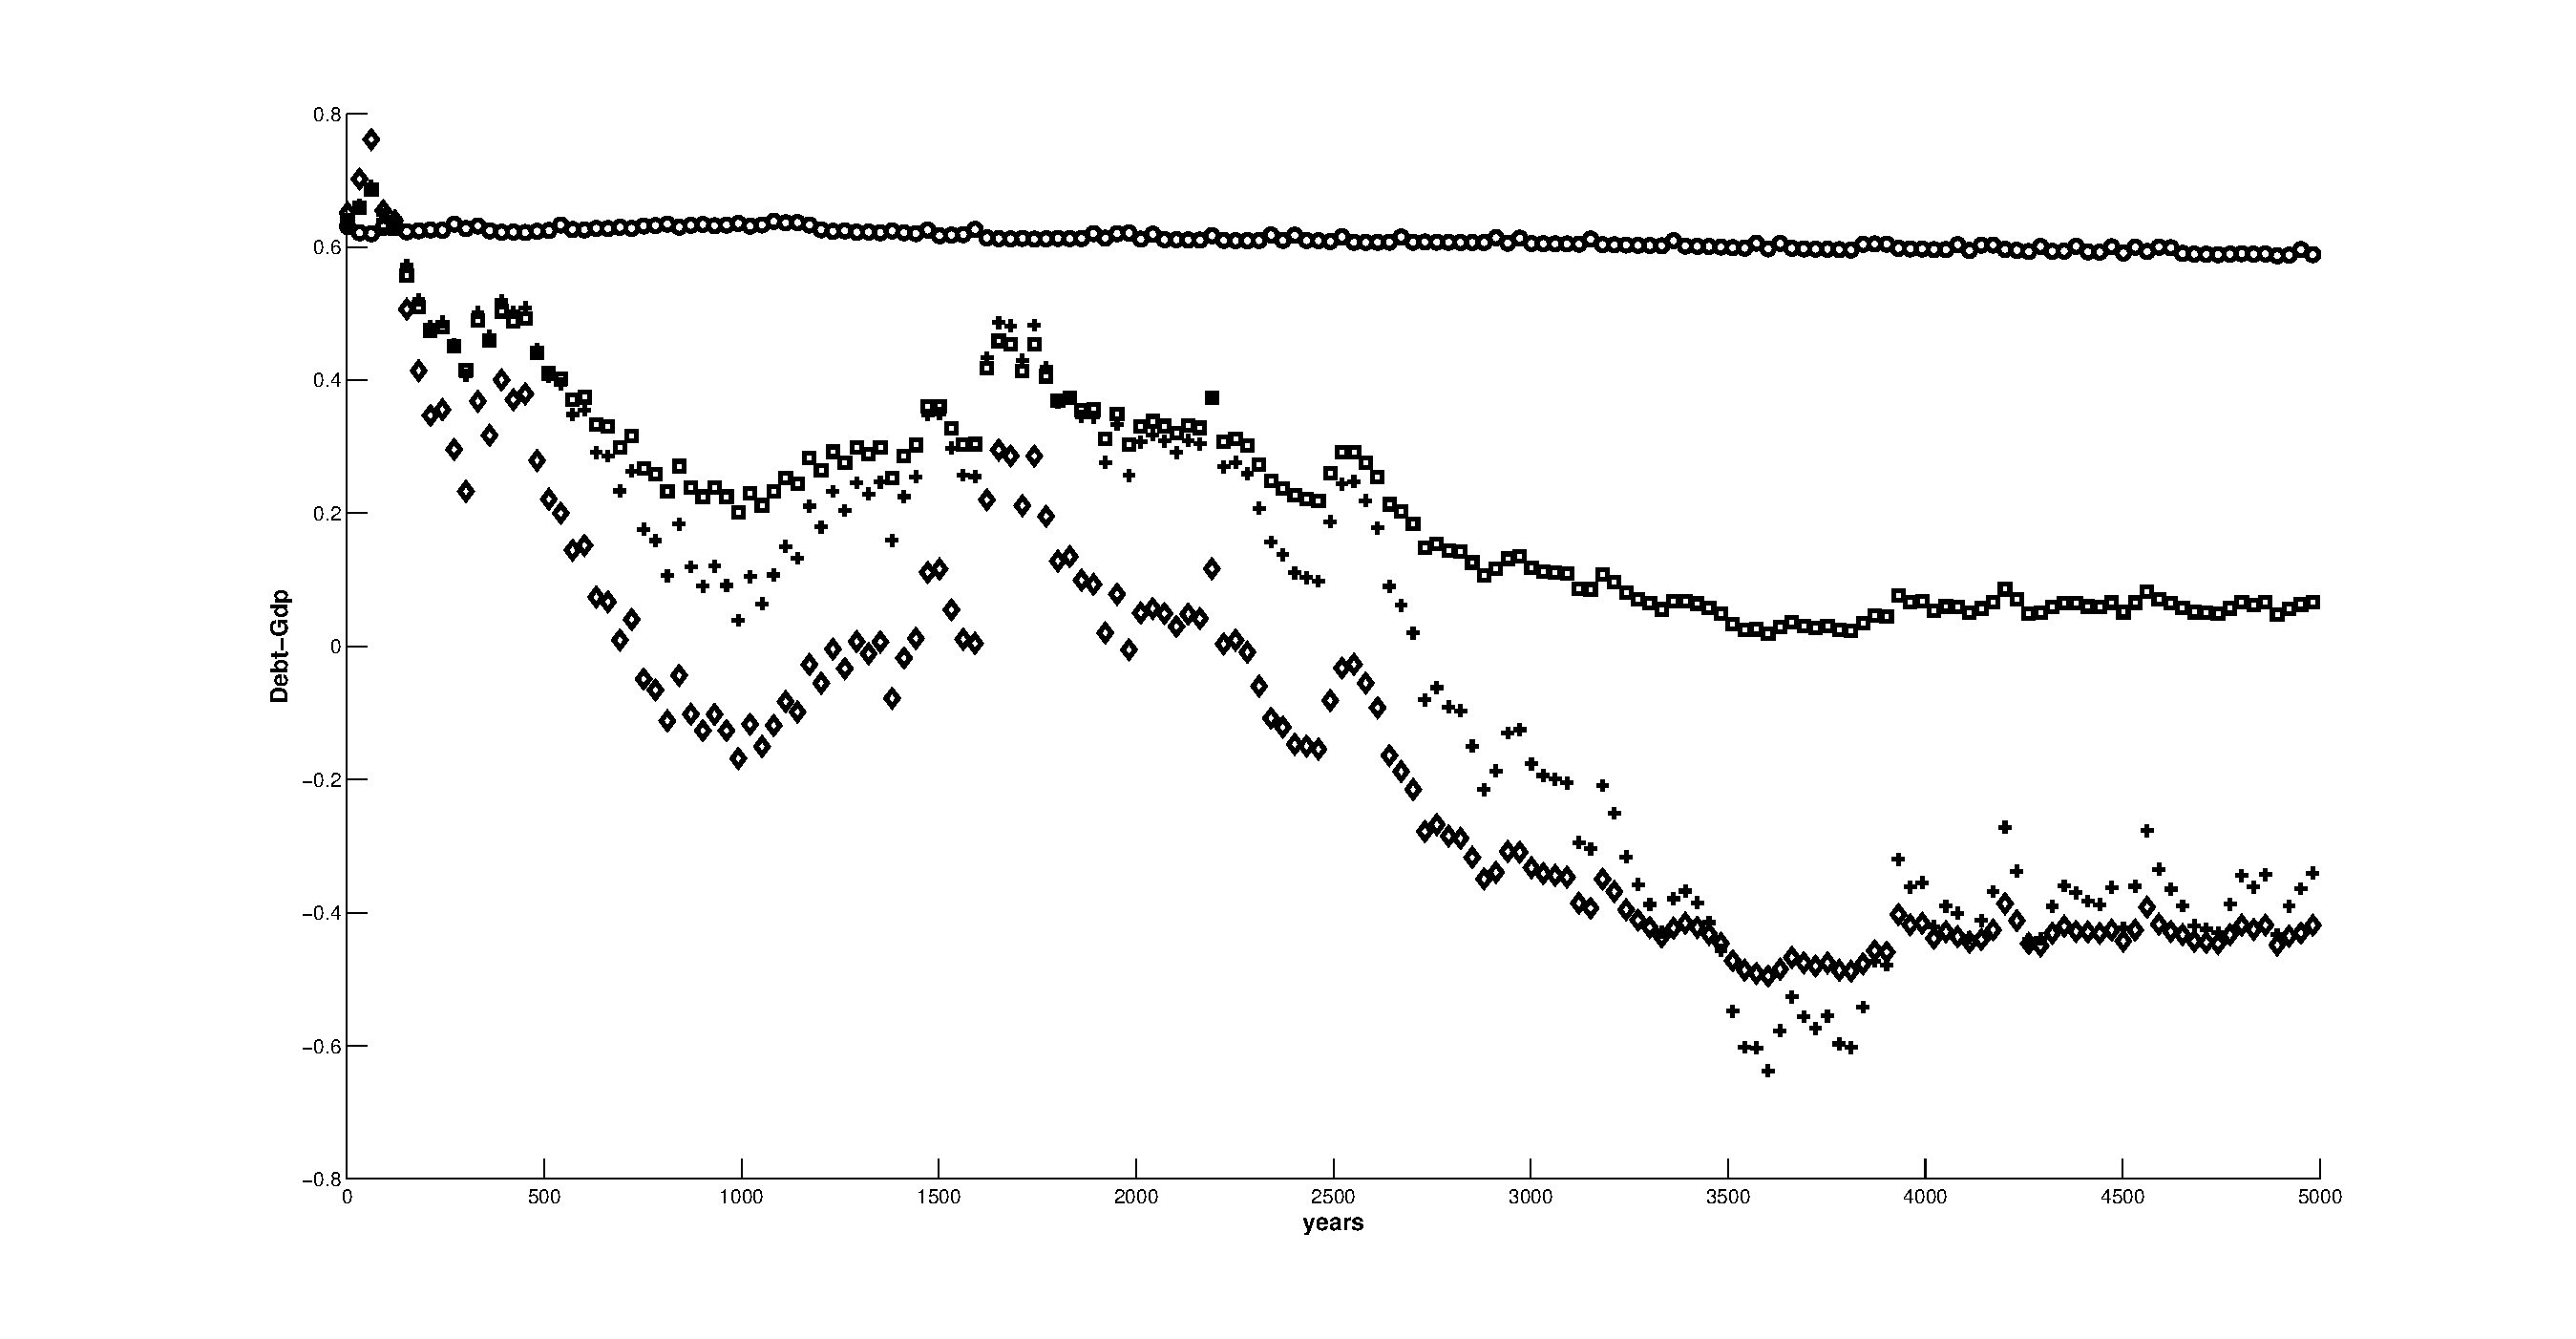
\includegraphics[width=\textwidth]{Draft25Graphs/LongSimulations.eps}
 \caption{Debt benchmark (o), acyclical interest rates (+), countercyclical interest rates ($(diamond$) and no inequality shocks \scriptsize ($\square$\normalsize) }
 %\caption{ Debt benchmark $\circle$, acyclical interest rates + , countercyclical interest rates $\diamond$ }% and no inequality shocks {\scriptsize $\square$ \normalsize}}
 \label{fig:LongSimulations}
 \end{figure}

\smallskip


In line with Section \ref{sec: SteadyStates}, all four economies the state $(x,\rho)$   converge to some long run
ergodic set, so that government debt and the tax rate converge to associated sets. When there are no discount factor shocks
(See lines with {$\diamond$, \scriptsize  $\square$ \normalsize}in figure \ref{fig:LongSimulations}) or small discount factor shocks that produce acyclical interest rates (line with + in figure \ref{fig:LongSimulations} )
the government has accumulated assets in this ergodic set. As alluded to in section \ref{sec: 2 agent example} %XXXXXX, \textcolor{red}{Please nail down the
 %section number.}
 the optimal policy adjusts  net asset
positions to ameliorate the two key constraints impinging  on the government policy, namely,
the inability to award agent-specific transfers (the restriction to \emph{affine taxes}) and the  absence of state-contingent assets (the
restriction to \emph {risk-free debt}). Starting from a point when the
relative assets of the low skilled agent (or the government if we use the
 normalization that sets $b_{2,t} = 0$) are low, extracting resources through lower
transfers exacerbates inequality. This is costly since the government has to
use higher taxes in future to redistribute. On the margin, the optimal policy requires the government (or low skill agent) to accumulate assets. But  interest rate
fluctuations interact with net asset positions to generate state-contingent  earnings
from assets. If interest rate are high when the government needs additional
revenues, accumulating assets relaxes the restriction imposed by absence
of state contingent assets. Thus, with countercyclical interest rates, these
forces reinforce each other, making the government's  long run asset position be positive.

In data, however, interest rates  generally decline in recessions. Procyclical interest rates mean that the
two forces outlined in the previous paragraph now oppose each other.  For  large enough interest rate fluctuations, this means that
the
government may want to accumulate debt. In Figure \ref{fig:LongSimulations}, the
black line represents the benchmark with discount factor shocks rigged to
replicate  procylical fluctuations in interest rates. For a particular initial condition for government debt,
the planner can refrain from varying debt for a very  long time.\footnote{Like the finding in Proposition \ref{prop: long run forces} for large discount factor shocks (in a way that interest rates are procylical)  there exist
regions where $x_t,\rho_t$ have low volatility and the  government is \emph{not} accumulating assets. But these
regions  are typically unstable. The two forces highlighted before that guide accumulation of assets now work in opposite direction and the net effect depends
on the relative strengths. In particular the sample paths from different initial conditions $\tilde{b}_{2,-1}$ (which would imply different choices for the initial $x_0,\rho_0)$ may display larger fluctuations in assets. However, at the calibrated initial conditions ($60\%$ debt-gdp ratio), the uncertainty associated with the mean path is very low for the first 5000 periods.}


Convergence to the ergodic region is  very slow.  With persistent shocks and an initial 60\% debt-GDP\ ratio,  it takes about 3,000 years for
the government to want to pay off all that debt
and then start accumulating assets. With
discount factor shocks, it takes even longer to repay the debt. It is still indebted after 5000 years. This confirms the comparative statics of the eigenvalues of linearized system in proposition \ref{prop: localstability}

Thus, the covariance of interest rates with fundamentals as emphasized in proposition \ref{prop: long run forces} substantially influences the ergodic distribution of government assets.
%\textcolor{red}{From Tom: the previous sentence needs improvement -- please weigh in.}

\subsubsection{Short run}

The analysis of the previous subsection studied  aspects of very low
frequency components of  the optimal policy. Here  we focus on business cycle frequencies.
 In our setting,  these higher frequency responses can conveniently be divided  into the magnitudes of changes as we switch from ``booms''
to ``recession,'' and the dynamics during  periods when recession or boom state persist.

We set the exogenous state
$s_0$ so  that we are in an outset of a recession.  Then we  solve the time 0 problem with identical initial conditions across
different settings. This pins down the initial state vector  $x_0,\rho_0$  that appears in our time $0$ Bellman equation.
We then use the policy rules to compute fluctuations of
different components in the government budget constraint across states. These responses
are summarized in Table \ref{tab:ShortRunPolicyResponses}. For each variable
$z$ in the table we report in the form $\Delta z\equiv \left( z\left(
s_l|x_0,\rho_0,s_0\right) -z\left( s_h|x_0,\rho_0,s_0\right) \right) /\bar{Y}
$ where $\bar{Y}$ is average undistorted - GDP \footnote{%
Note that predetermined variables like repayment on existing debt drop out
of the accounting and we have
\begin{equation*}
\Delta [g]+\Delta[T]+ \Delta [B]=\Delta[\tau \theta_1 l_1]+ \Delta[\tau
\theta_2 l_2]
\end{equation*}%
}.

%\smallskip Table ???\ reports standard deviation and persistence of all
%variables in table ???-1.


%\textcolor{red}{Tom XXXXX: do some more rewriting of the following.}\textcolor{green}{David:  Agreed I think some signs were flipped tried a small rewrite} \textcolor{red}{XXXXXX: Nice job David. I did some minor writing touchups.}
The source of shocks is very important. Three different types of shocks
that produce similar drops in GDP  have very different consequences for optimal policies, both qualitatively and
quantitatively. %Note that there are significant qualitative and quantitative
%differences between TFP\ shock vs TPF and inequality shock.
In the benchmark, the government responds to a shock by a making big increases in transfers, the  tax rate, and  government debt. However, without inequality shocks (row 4), the government
responds by decreasing transfers and  increasing both debt and
the tax rate, but by an amount an order of magnitude smaller than the benchmark. This  indicates that ignoring distributional goals can produce a misleading view about  optimal government
policy in recessions.



\begin{table}[tbp]
\begin{tabular}{|l|c|c|c|c|c|c|c|}
\hline
& \textbf{$\Delta g$} & \textbf{$\Delta B$} & \textbf{$\Delta T$} & \textbf{$%
\Delta [\tau\theta_1l_1]$} & \textbf{$\Delta [\tau\theta_2l_2]$} & \textbf{$%
\Delta Y$} & \textbf{$\Delta \tau$} \\ \hline
\textbf{Benchmark} & 0.0000 & -1.1561 & 0.6871 & -0.1593 & -0.3096 & -2.8536
& 0.3732 \\ \hline
\textbf{Acyclical Interest Rates} & 0.0000 & -1.1126 & 0.6591 & -0.1497 &
-0.3038 & -2.8613 & 0.3879 \\ \hline
\textbf{Countercyclical Interest Rates} & 0.0000 & -1.0794 & 0.6387 & -0.1415 &
-0.2992 & -2.8677 & 0.3997 \\ \hline
\textbf{No Inequality} & 0.0000 & -0.1380 & -0.5459 & -0.5635 & -0.1204 &
-2.6294 & 0.0622 \\ \hline
\textbf{Expenditure Shocks} & -7.5037 & 2.9137 & 2.8612 & -1.3759 & -0.3530 & -2.3443 &
-1.1598 \\ \hline
\end{tabular}%
\caption{The tables summarizes the changes in the different components of the government budget as we transit from ``boom'' to a ``recession''.  All numbers are normalized by un-distorted GDP except $\protect\tau $
}

\label{tab:ShortRunPolicyResponses}
\end{table}
\smallskip
Discount factor shocks have  minor effects on impact and matter more for
transient dynamics that ultimately have big long run  effects.
Figures \ref{fig:DiscoutFactorComparison} and \ref%
{fig:DiscoutFactorComparison2} show how the transient dynamics for prolonged
booms (or recessions)  differ with and without discount factor shocks.
The four panels have taxes, transfers, debt and interest rate movements for
a path of 25 years.
The bold lines in figures \ref{fig:DiscoutFactorComparison} and \ref{fig:DiscoutFactorComparison2} refer to the benchmark (with procylical interest rates) and
 the version with acyclical interest rates, respectively. The dotted line in both the figures is the version with countercyclical interest rates. The shaded regions
are periods with low output. We see that in a prolonged booms, the
government accumulates assets and that it lowers the tax rate when there are no discount
factor shocks.
%
% \FRAME{ftbpFU}{5.0652in}{2.853in}{0pt}{\Qcb{Optimal response in a benchmark
% (solid line) and a model with no discount factor shocks (dotted line).}}{%
% \Qlb{fig:DiscoutFactorComparison}}{discoutfactorcomparison.tif}{\special%
% {language "Scientific Word";type "GRAPHIC";maintain-aspect-ratio
% TRUE;display "USEDEF";valid_file "F";width 5.0652in;height 2.853in;depth
% 0pt;original-width 12.5934in;original-height 7.0629in;cropleft "0";croptop
% "1";cropright "1";cropbottom "0";filename
% 'Draft25Graphs/DiscoutFactorComparison.tif';file-properties "XNPEU";}}
%
% \FRAME{ftbpFU}{4.9822in}{2.8565in}{0pt}{\Qcb{Optimal response in a benchmark
% (solid line) and a model with interest rate fluctuations (dotted line).}}{%
% \Qlb{fig:DiscoutFactorComparison2}}{discoutfactorcomparison2.tif}{\special%
% {language "Scientific Word";type "GRAPHIC";maintain-aspect-ratio
% TRUE;display "USEDEF";valid_file "F";width 4.9822in;height 2.8565in;depth
% 0pt;original-width 12.3858in;original-height 7.0733in;cropleft "0";croptop
% "1";cropright "1";cropbottom "0";filename
% 'Draft25Graphs/DiscoutFactorComparison2.tif';file-properties "XNPEU";}}%
%
\smallskip

\begin{figure}[htp]
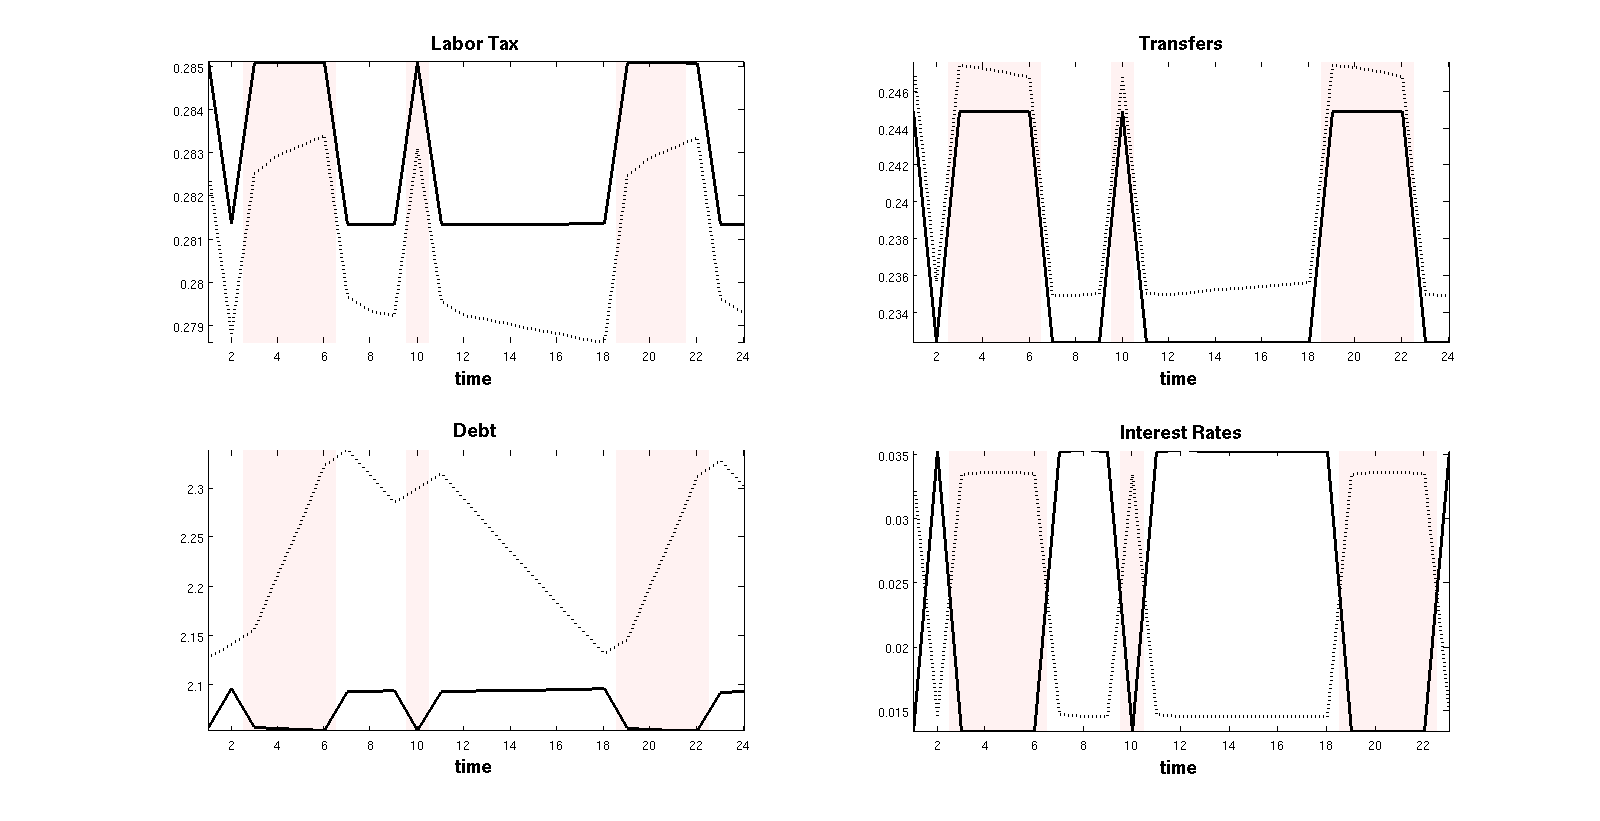
\includegraphics[width=\textwidth]{Draft25Graphs/DiscoutFactorComparison.png}
\caption{This plots a typical sample path taxes, transfers,debt and interest rates. The bold lines are with  benchmark calibration and the dotted lines refer to the variant with countercyclical interest rates. The shaded regions are recessions.}
\label{fig:DiscoutFactorComparison}
\end{figure}

\begin{figure}[htp]
\centering
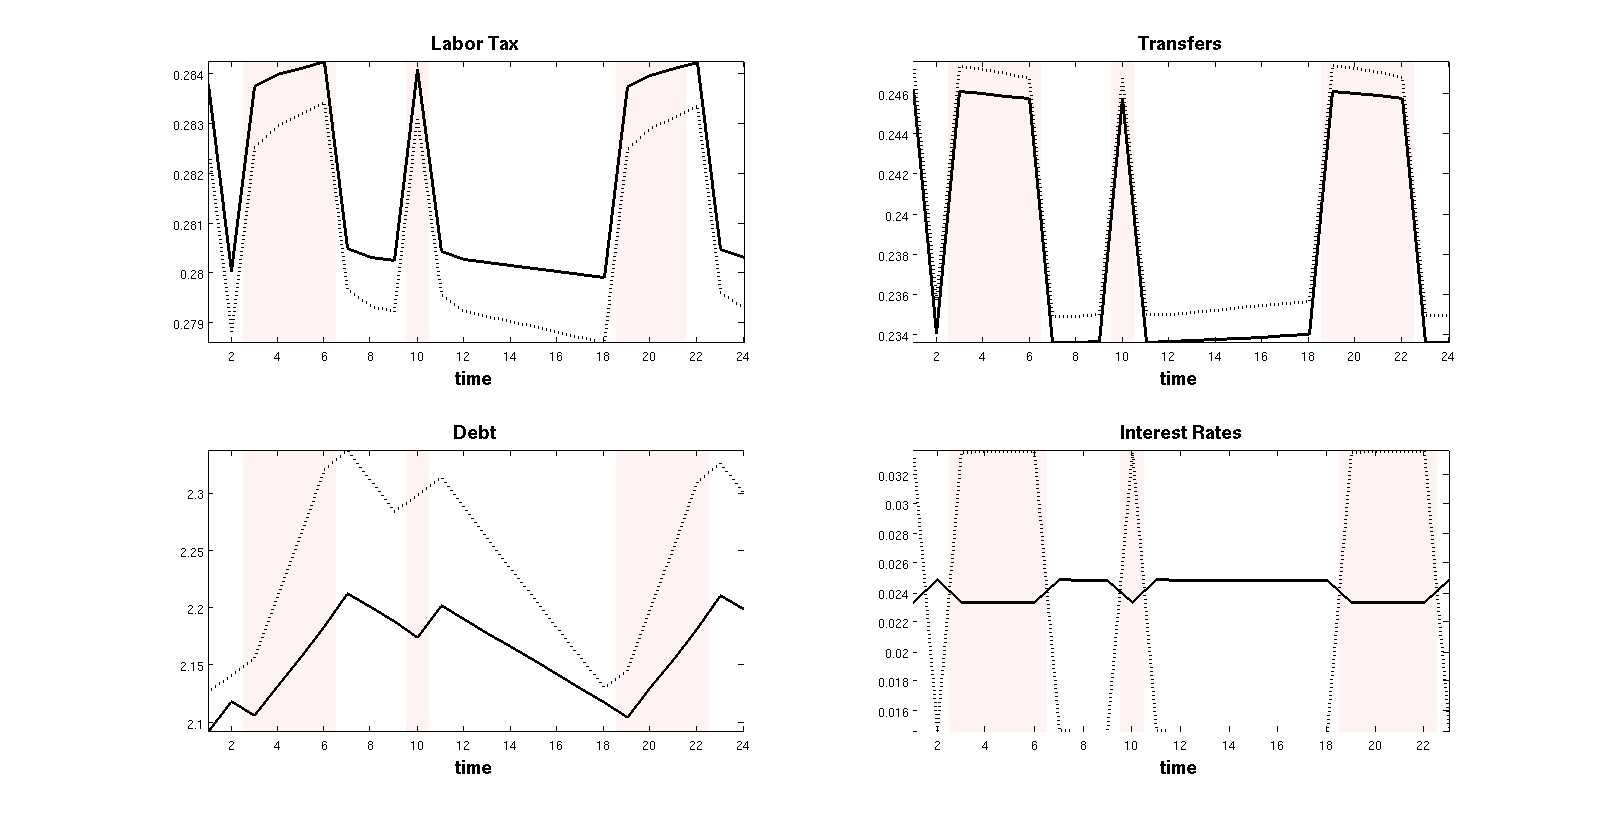
\includegraphics[width=\textwidth]{Draft25Graphs/DiscoutFactorComparison2.png}
\caption{This plots a typical sample path taxes, transfers, debt and interest rates.  The bold lines  are with acyclical interest rates calibration and the dotted lines correspond to the case with countercyclical interest rates. The shaded regions are recessions.}
\label{fig:DiscoutFactorComparison2}
\end{figure}

\smallskip


\section{Concluding remarks\label{sec:conclude}}

  The spring of 2013 witnessed a heated debate in newspapers and economic magazines about the accuracy and meaning of empirical  correlations between output growth rates and
ratios of government debt to GDP and  in data sets assembled by \cite{Reinhart2010}.
From the  perspectives of our paper and of  \cite{Wer07a}, those correlations and those debates are especially difficult to interpret
because in our settings, total government debt is not a relevant state variable that affects allocations, government transfers, or tax rates.
The principal message of our paper  is that  without exogenous restrictions on transfers, the level of government debt is not what matters. What
 does matter is how government  debt is distributed among people relative to society's attitudes toward unequal allocations of consumption and labor.  Using a recursive representation that works with a correct state variables --- a vector of marginal utility adjusted net asset positions and a vector of pairwise ratios of marginal utilities  --  we have
 presented  a sequence of examples designed to show how  agents net positions affect optimal government policies for choosing distorting tax
 rates, transfers, and government issues or holdings of risk-free bonds. We find that a significant determinant of an optimal asymptotic government
 debt or government debt-GDP ratio is how interest rate risk is correlated with risks to fundamentals that threaten to widen or narrow
 inequality in after-tax and after-transfer incomes. To interpret those Reinhart-Rogoff facts country-by-country, we would
 want to know much more about the distribution of net assets across people within each country and how they interact with interest rate risks and other risks.

\smallskip

\smallskip

\smallskip

\pagebreak

\smallskip %
%[\textbf{MG: I would delete the remaining section or have their short
%informal summary}]\smallskip
%
%\subsection{\protect \smallskip History-dependent taxes when asset taxes are
%not available\label{Sec: retroactive}}
%
%\smallskip
%
%The optimal tax schedule described in section \ref{sec:tax_opt_all} requires
%that the government can observe and tax assets of the households. When the
%government can do that, all impediments to optimality coming from
%preexisting debts and market incompleteness vanish. In period 0, the
%government can effectively redistribute assets as it wants and then can use
%asset taxes to assure that the distribution of assets never changes. There
%is never a distribution of asset holdings that is inefficient or that
%prevents the government from achieving the constrained optimal allocation.
%
%One objection to this characterization of an optimal tax policy is that in
%practice asset holdings of the households are not easily observed because
%many financial transactions are anonymous and hidden from the government.
%That makes taxation of assets difficult. In this section, we discuss the
%implications for optimal taxation that follow from a government's inability
%to tax assets when nevertheless it has access to an arbitrary non-linear tax
%$T_{t}\left( y_{t},...,y_{0}\right) $. Since consumption taxes can replicate
%asset taxes, we rule them out.
%
%\smallskip In the appendix, we state an optimal tax problem for general
%non-linear labor income taxes $T_{t}\left( y_{t},...,y_{0}\right) .$ We also
%characterize a particular example that exhibits the same features
%encountered in Section \ref{Sec: snl}, namely, that distortions and
%allocations generally depend on the history of past shocks and the initial
%distribution of net assets $\left \{ \tilde{b}_{i,-1}\right \} _{i=2}^{I}.$
%The example is basically a variant of the AMSS-like economy of Section \ref%
%{Sec: quasi-linear with risk aversion} where both agents can now work. We
%show that in that economy either the consumption of agent 1, $c_{1,t},$ must
%eventually hit the lower bound, as in the case of affine taxes, or the
%consumption of agent 2, $c_{2,t}$ must initially fluctuate but eventually
%converge to a constant. Both of those cases imply that optimal taxes and
%allocations depend not only on the current $g$ but also on its history.
%
%\smallskip
%
%\subsection{Role of debt markets?}
%
%\smallskip
%
%Proposition \ref{Prop: mechdes decentralize} shows that debt markets play no
%useful role when taxes are sufficiently flexible, and in particular when
%they can depend on the entire history of labor earnings. For then the
%government can effectively shut the debt market by taxing away all income if
%it observes that the agent uses this market. The government can then provide
%all insurance through the tax code.
%
%An optimal tax schedule can be less extreme. Various decentralizations
%popular in the literature use a continuous but non-linear tax on asset
%income, such as Werning (2012) or XXXX. Despite being continuous, these
%taxes effectively achieve the same goal as attained in the extreme example
%in Proposition \ref{Prop: mechdes decentralize}: they make it prohibitively
%costly for agents to depart from the allocation assigned by the planner.
%This result is not surprising, for it is known (see, for example, Golosov
%and Tsyvinski (2007)) that welfare in the mechanism design problems is lower
%when agents can trade freely or face linear returns on assets.
%
%In the economy with affine taxes considered in section \ref{Sec:
%quasi-linear with risk aversion}, debt markets played an important role.
%They allowed the agents and the government to smooth consumption and
%distortions in response to the aggregate shocks.
%
%The contrasting roles of debt markets in these two situations induces us to
%ask, ``when are debt markets useful?'' In general, unrestricted debt markets
%play two roles, one that is welfare decreasing, another that is welfare
%enhancing. Optimal non-linear income taxes are generally not convex. When
%agents can freely trade assets, they can convexity their budget sets. On the
%one hand, private asset trading improves the utility of each individual
%agent but it reduces the government's ability to redistribute and therefore
%lowers social welfare. This is why in the mechanism design problems it is
%welfare decreasing for agents to trade behind the planner's back. On the
%other hand, when the tax system is less than perfect, trading assets usually
%cannot provide an agent with an optimal amount of consumption smoothing. The
%affine taxes in section \ref{Sec: quasi-linear with risk aversion}
%illustrate that. If agents could not trade among themselves, consumption of
%the risk averse agent, $c_{2,t},$ would fluctuate much more, leading to
%welfare losses.
%
%Allowing taxes on current income to be non-linear, as in Section \ref{Sec:
%snl}, helps the government provide more insurance to agents through the tax
%code, although less than perfectly. As a result, whether welfare is higher
%in the economy in which agents can trade assets freely or in the economy in
%which agents cannot trade assets depends on which force dominates. It is
%easy to construct examples in which one or the other of these economies has
%higher welfare depending on the redistributive objectives of the government
%or the nature of the aggregate shocks. [\textbf{should we actually put an
%example of that?}] This highlights a general point. The more restricted is
%the available set of tax instruments, the more important it is for the
%agents to be able to trade assets freely. We conjecture that this point
%would be more important in economies with richer shock structures.
%%such as additional shocks to TFP, the distribution of
%%skills, or idiosyncratic shocks.
%
%\smallskip

\smallskip

\smallskip \pagebreak

\smallskip

\section{Appendix}

\subsection{Additional details for Section \ref{Sec: extensions}}
\label{appndx: borrowing constraints example}
In this section we construct an example in which the government can achieve
higher welfare in the economy with ad-hoc borrowing limits.  We restrict ourselves to $I=2$, $\theta_1>\theta_2=0$, quasilinear preferences for Agent 1 : $U^1(c,l)=c-h(l)$ and a concave utility function (that satisfies Inada conditions) for Agent 2

\smallskip

Suppose that $g_{t}=0$ and $\beta_t=\beta$ for all $t,$ so that the economy is deterministic. In addition, assume that $\underline{b}_{1}=0$ and $\underline{b}_{2}=-\infty .$ Given $\left( \beta ^{-1}{b}_{1,-1},\beta ^{-1}{b}%
_{2,-1},\beta ^{-1}{B}_{-1}\right) $, the optimal policy solves :

\begin{equation}
 \label{obj: borrowingconstexample}
 \max_{\left \{ c_{1,t},c_{2,t},l_{1,t},b_{1,t},b_{2,t},R_{t}\right \}
_{t}}\sum_{t=0}^{\infty }\beta ^{t}\left[ \alpha _{1}\left(
c_{1,t}-h(l_{1,t})\right) +\alpha _{2}U^2(c_{2,t})\right]
 \end{equation}
subject to

\begin{subequations}
 \begin{equation}
 \label{eq:borrowingconstexample-imp}
c_{2,t}-c_{1,t}+b_{2,t}-b_{1,t}+h^{\prime }(l_{1,t})l_{1,t}=R_{t-1}\left(
b_{2,t-1}-b_{1,t-1}\right)
 \end{equation}
 \begin{equation}
 \label{eq:borrowingconstexample-res}
 c_{1,t}+c_{2,t}\leq \theta l_{1,t}
 \end{equation}
\begin{equation}
 \label{eq:borrowingconstexample-euler1a}
 1\geq \beta R_t
 \end{equation}
 \begin{equation}
 \label{eq:borrowingconstexample-euler1b}
 (1-\beta R_t)b_{1,t}=0
 \end{equation}
 \begin{equation}
 \label{eq:borrowingconstexample-euler2}
 U^2_{c,t}=\beta R_t U^2_{c,t+1}
 \end{equation}
 \begin{equation}
 \label{eq:borrowingconstexample-limits}
 b_{1,t}\geq0
 \end{equation}
\end{subequations}

We solve this maximization problem in two stages. First, we solve the 
problem  (\ref{obj: borrowingconstexample}) for a fixed sequence of $\left \{ R_{t}\right \} _{t}.$ Denote
the value of the objective function for the reduced problem by $W\left(
\left \{ R_{t}\right \} _{t}\right) .$ Second choose $\ \left \{ R_{t}\right \} _{t}$ to maximize $W\left( \left \{ R_{t}\right \} _{t}\right)$.

\noindent Let $\mu_t\beta^t \Pr(s^t)$ be the Lagrange multiplier associated with the constraint (\ref{eq:borrowingconstexample-imp}).
 \begin{lemma}
 For $R_t=\beta^{-1}$, we can choose a  time invariant solution  $c_{1,t}= \bar{c}_{1},c_{2,t}=\bar{c}_{2},l_{1,t}=\bar{l}%
_{1},b_{1,t}=\bar{b}_{1},b_{2,t}=\bar{b}_{2}$ to the relaxed problem that satisfies
\begin{equation*}
\bar{b}_{2}-\bar{b}_{1}=\bar{b}_{2}=\bar{b}_{2,-1}-\bar{b}_{1,-1}.
\end{equation*}

\end{lemma}
\begin{proof}
  By Theorem \ref {theorem: main}, we can set $b_{1,t}=0$  and ignore constraint (\ref{eq:borrowingconstexample-limits}). Further ignoring constraint (\ref{eq:borrowingconstexample-euler2}), a stationary interior solution is given by

 \begin{subequations}
 \begin{equation}
  \label{eq:borrowingconstexample-foc-c2}
U^2_c(\bar{c}_2)=\frac{2\bar{\mu}+\alpha_1}{\alpha_2}
 \end{equation}
\begin{equation}
\label{eq:borrowingconstexample-foc-labor}
\alpha_1 h'(\bar{l}_1)=\theta_1\alpha_1+\bar{\mu}[\theta_1-h''(\bar{l}_1)\bar{l}_1-h'(\bar{l}_1)]
 \end{equation}
\begin{equation}
\label{eq:borrowingconstexample-foc-b_2}
b_{2,-1}=\frac{2\bar{c}_2+ \bar{l}_1\left[h'(\bar{l}_1)-\theta_1 \right] }{\beta^{-1}-1}
\end{equation}

 \end{subequations}


Note that if a solution to the above set of equations exists, (\ref{eq:borrowingconstexample-euler2}) is naturally satisfied.

We first establish some comparative statics with respect to $\bar{\mu}$. It is easy to see that concavity of $U^2$ implies $\frac{\partial \bar{c}_2}{\partial \mu}<0$. Further equation (\ref{eq:borrowingconstexample-foc-labor}) can be rearranged to get

 \[\frac{h'(\bar{l}_1)}{\theta_1}=\frac{\alpha_1+\bar{\mu}}{\left[\alpha_1+\bar{\mu}+\bar{\mu}\left(\frac{h''(\bar{l}_1)\bar{l}_1}{h'(\bar{l}_1)}\right)\right]}\]

 Using convexity of $h$ we have $\frac{\partial \bar{l}_1}{\partial \mu}<0$.

 As $\bar{\mu}\to -\frac{\alpha_1}{2}$, the RHS of (\ref{eq:borrowingconstexample-foc-b_2}) approaches $+\infty$ and $\bar{\mu}\to + \infty$ it approaches some $\underline{b}_2<0$. Thus we have a stationary solution for a range of $b_{2,-1}$.

\end{proof}

\begin{lemma}
 For $R_t=\beta^{-1}$, if $b_{2,-1}<b_{1,-1}$ then $\bar{\mu}>0$
\end{lemma}
\begin{proof}
 Suppose $\bar{\mu}\leq0$ when $b_{2,-1}<b_{1,-1}$.  At $\mu=0$, $h'(\bar{l}_1)=\theta_1$  and the RHS of (\ref{eq:borrowingconstexample-foc-b_2}) is positive.  At $\mu<0$ we have $h'(\bar{l}_1)>\theta_1$ . The observations above imply that the RHS of (\ref{eq:borrowingconstexample-foc-b_2}) is increasing in $\mu$ and this clearly violates equation (\ref{eq:borrowingconstexample-foc-b_2}).  Thus we have a contradiction.
 \end{proof}
\smallskip

When $R_{t}=1/\beta $ for all $t,$
the solution of the reduced problem is an optimal allocation for an economy
in which agents face no borrowing constraints

Let $\left. \frac{\partial }{\partial R_{1}}W\left( \left \{ R_{t}\right \}
_{t}\right) \right \vert _{\left \{ R_{t}\right \} =\bm{\beta }^{-1}}$
be the derivative of $W\left( \left \{ R_{t}\right \} _{t}\right) $ with
respect to $R_{1}$ evaluated at $R_{t}=\beta ^{-1}$ for all $t$. The multiplier on constraints  (\ref{eq:borrowingconstexample-euler1b}) and (\ref{eq:borrowingconstexample-euler2}) are zero and let $\xi_t\geq0$ be the multiplier on constraint (\ref{eq:borrowingconstexample-euler1a}). Our
observations above imply that
\begin{equation*}
\left. \frac{\partial }{\partial R_{1}}W\left( \left \{ R_{t}\right \}
_{t}\right) \right \vert _{\left \{ R_{t}\right \} =\bm{\beta }^{-1}}=%
\bar{\mu}\bar{b}_{2,t}-\xi_1\leq\bar{\mu}\left( \bar{b}_{2,-1}-\bar{b}%
_{1,-1}\right) <0
\end{equation*}
and therefore $R_{t}=\beta ^{-1}$ for all $t$ is not the optimal equilibrium
sequence. Therefore, welfare in the economy with exogenous borrowing
constraints is strictly higher than in the economy without exogenous
borrowing constraints.\footnote{%
The mechanism in this example is similar to a finding of \cite{Yared2012}, who
showed that relaxing agents' borrowing constraints can be suboptimal in an
economy with idiosyncratic shocks. Our analysis shows that this insight is
more general and holds even in economies with no shocks.}

The outcome that welfare can be strictly higher with exogenous borrowing
constraints depends on our assumption that agents do not face idiosyncratic risk. If agents were also subject to idiosyncratic shocks,
exogenous borrowing constraints would have the additional effect of limiting
agents' ability to self-insure against those shocks.\footnote{%
See \cite{Aiyagari1998} and \cite{Heathcote2005} for details.}
Nevertheless, the insight from the example carries through that even though exogenous
borrowing constraints can hurt agents' to insure against idiosyncratic shocks, they
can help a government smooth distortions with respect to aggregate shocks
like government expenditure shocks.



\smallskip
\subsection{\smallskip Proof of Proposition  \ref{prop: affine eqm nec and suff}}
\label{appndx: affine eqm nec and stuff}
\smallskip

We prove a slight more general version of our result. Consider an infinite
horizon, incomplete markets economy in which an agent maximizes utility
function $U:\mathbb{R}_{+}^{n}\rightarrow \mathbb{R}$ subject to an infinite
sequence of budget constraints. We assume that $U$ is concave and
differentiable. Let $\bm{a}(s^t)$ be a vector of $n$ goods and let $%
\bm{p}(s^{t})$ be a price vector in state $s^{t}$ with $p_{i}(s^{t})$
denoting the price of good $i.$ We use a normalization $p_{1}\left(
s^{t}\right) =1$ for all $s^{t}.$ There is a risk-free bond.

Let $b(s^{t})$ be the agent's bond holdings, and let $\bm{e}\left(
s^{t}\right) $ be a stochastic vector of endowments.

\textbf{Consumer maximization problem}


\begin{equation}
\max_{\bm{a}_{t},b_{t}}\sum_{t=0}^{\infty }\bigl[\Pi_{j=0}^t \beta(s_j)\bigr]\Pr \left(
s^{t}\right) U(\bm{a}\left( s^{t}\right) )
\label{Tech appendix: consumer maximization}
\end{equation}%
subject to%
\begin{equation}
\bm{p}\left( s^{t}\right) \bm{a}\left( s^{t}\right) +q(s^{t})b\left(
s^{t}\right) =\bm{p}\left( s^{t}\right) \bm{e}\left( s^{t}\right)
+b\left( s^{t-1}\right)  \label{Tech appendix: budget constraint}
\end{equation}%
and $\left \{ b\left( s^{t}\right) \right \} $ is bounded and $\left \{
q(s^{t})\right \} $ is the price of the risk-free bond.

The Euler conditions are%
\begin{eqnarray}
\bm{U}_{a}(s^{t}) &=&U_{1}(s^{t})\bm{p}(s^{t})
\label{Tech appendix: Euler} \\
\Pr \left( s^{t}\right) U_{1}\left( s^{t}\right) q(s^{t}) &=&\beta(s_t)
\sum_{s^{t+1}>s^{t}}\Pr \left( s^{t+1}\right) U_{1}\left( s^{t+1}\right) .
\notag
\end{eqnarray}

\begin{lemma}
\smallskip Consider an allocation $\left \{ \bm{a}_{t},b_{t}\right \} $
that satisfies (\ref{Tech appendix: budget constraint}), (\ref{Tech
appendix: Euler}) and $\left \{ b_{t}\right \} _{t}$ is bounded. Then $%
\left
\{ \bm{a}_{t},b_{t}\right \} $ is a solution to (\ref{Tech
appendix: consumer maximization}).
\end{lemma}

\begin{proof}
The proof follows closely \cite{Constantinides1996}. Suppose there is
another budget feasible allocation $\bm{a}+\bm{h}$ that maximizes (%
\ref{Tech appendix: consumer maximization}). Since $U$ is strictly concave,
\begin{eqnarray}
&&\mathbb{E}_{0}\sum_{t=0}^{\infty }\bigl[\Pi_{j=0}^t \beta(s_j)\bigr]U(\bm{a}_{t}+\bm{h}%
_{t})-\mathbb{E}_{0}\sum_{t=0}^{\infty }\bigl[\Pi_{j=0}^t \beta(s_j)\bigr]U(\bm{a}_{t})
\label{Tech appendix: gain from h} \\
&\leq &\mathbb{E}_{0}\sum_{t=0}^{\infty }\bigl[\Pi_{j=0}^t \beta(s_j)\bigr]\bm{U}_{a}(\bm{a}%
_{t})\bm{h}_{t}  \notag
\end{eqnarray}

To attain $\bm{a}+\bm{h}$, the agent must deviate by $\varphi _{t}$
from his original portfolio $b_{t}$ such that $\left\{ \varphi _{t}\right\}
_{t}$ is bounded$,$ $\varphi _{-1}=0$ and
\begin{equation*}
\bm{p}(s^{t})\bm{h}\left( s^{t}\right) =\varphi
(s^{t-1})-q(s^{t})\varphi (s^{t})
\end{equation*}%
Multiply by $\bigl[\Pi_{j=0}^{t-1} \beta(s_j)\bigr]\Pr \left( s^{t}\right) U_{1}(s^{t})$ to get:%
\small
\begin{eqnarray*}
\bigl[\Pi_{j=0}^{t-1} \beta(s_j)\bigr] \Pr \left( s^{t}\right) U_{1}(s^{t})\bm{p}(s^{t})\bm{h}%
\left( s^{t}\right)  &=&\bigl[\Pi_{j=0}^{t-1} \beta(s_j)\bigr]\Pr \left( s^{t}\right)
U_{1}(s^{t})\varphi (s^{t-1})-q(s^{t})\bigl[\Pi_{j=0}^{t-1} \beta(s_j)\bigr] \Pr \left( s^{t}\right)
U_{1}(s^{t})\varphi (s^{t}) \\
&=&\bigl[\Pi_{j=0}^{t-1} \beta(s_j)\bigr] \Pr \left( s^{t}\right) U_{1}(s^{t})\varphi (s^{t-1})-\bigl[\Pi_{j=0}^{t-1} \beta(s_j)\bigr]\beta(s_t)\sum_{s^{t+1}>s^{t}}\Pr \left( s^{t+1}\right) U_{1}\left(
s^{t+1}\right) \varphi (s^{t})
\end{eqnarray*}%
\normalsize
where we used the second part of (\ref{Tech appendix: Euler}) in the second
equality. Sum over the first $T$ periods (pathwise) and use the first part of (\ref {Tech appendix: Euler}) to eliminate $\bm{U}_{a}(\bm{a}%
_{t})=U_{1}(s^{t})\bm{p}(s^{t})$%
\begin{equation*}
\sum_{t=0}^{T}\bigl[\Pi_{j=0}^{t-1} \beta(s_j)\bigr] \Pr \left( s^{t}\right) \bm{U}_{a}(\bm{a}%
_{t})\bm{h}\left( s^{t}\right) =-\bigl[\Pi_{j=0}^{T} \beta(s_j)\bigr] \sum_{s^{T+1}>s^{T}}\Pr
\left( s^{T+1}\right) U_{1}\left( s^{T+1}\right) \varphi (s^{T}).
\end{equation*}%
Since $\left\{ \varphi _{t}\right\} _{t}$ is bounded there must exist $\bar{%
\varphi}$ s.t. $|\varphi _{t}|\leq \bar{\varphi}$ for all $t$. By Theorem
5.2 of Magill and Quinzii (1994), this equilibrium with debt constraints
implies a transversality condition on the right hand side of the last
equation, so by transitivity we have%
\begin{equation*}
\lim_{T\rightarrow \infty }\sum_{t=0}^{T}\bigl[\Pi_{j=0}^{t-1} \beta(s_j)\bigr]\Pr \left( s^{t}\right)
\bm{U}_{a}(\bm{a}_{t})\bm{h}\left( s^{t}\right) =0.
\end{equation*}%
Substitute this into (\ref{Tech appendix: gain from h}) to show that $%
\bm{h}$ does not improve utility of consumer.
\end{proof}

\smallskip
% 
% \subsection{Proof of Proposition \protect\ref{prop: quasilinear noninterior}}
% 
% \smallskip Let $\alpha _{2}$ be the Pareto weight on the unproductive agent.
% Given a (initial) net distribution of assets $\tilde{b}_{2}=b_{2}-b_{1}$ the
% optimal solution solves the following Bellman equation.
% 
% \begin{equation}
% V(\beta^{-1}\tilde{b}_2,s\_)=\max_{c_1(s),c_2(s),l_1(s),\tilde{b}_2^{\prime }(s)}
% \sum_{s}\Pr(s|s\_) \left \{ (1-\alpha_2)\left(c_1(s)-h[l_1(s)]\right)+\alpha_2
% c_2(s) +\beta V(\beta^{-1} \tilde{b}^{\prime }_2(s),s)\right\}
% \label{eq:QuasiLinearProblem}
% \end{equation}
% 
% subject to
% \begin{subequations}
% \begin{equation}
% c_2(s)-c_1(s)+\tilde{b}^{\prime }_2(s)+ l_1(s)h^{\prime }[l_1(s)]=\frac{%
% \tilde{b}_2}{\beta}  \label{eq:QLImp}
% \end{equation}
% \begin{equation}
% c_2(s)+c_1(s)+g(s)\leq\theta_1l_1(s)  \label{eq:QLResource}
% \end{equation}
% 
% \begin{equation}
% c_1(s)\geq 0\quad c_2(s)\geq0  \label{eq:QLconsbounds}
% \end{equation}
% \begin{equation}
% \tilde{b}_2^{\prime }(s)\in [\underline b,\bar b]
% \end{equation}
% 
% Let $\mu(s)\Pr(s|s\_) , \xi(s)\Pr(s|s\_)$ , $\lambda^{c_i}(s)\Pr(s|s\_)$ be the
% multipliers on the implementability (\ref{eq:QLImp}), resource constraint (\ref{eq:QLResource}) and the non-negativity constraints (\ref{eq:QLconsbounds})
% for the respective consumption. For now we assume that $\underline b$ and $%
% \bar b$ are natural debt limits and ignore them on the equilibrium path. The
% FONCs of the problem are
% \end{subequations}
% 
% \begin{subequations}
% \begin{equation}
% 1-\alpha_2+\mu(s)+ \lambda^{c_1}(s)-\xi(s)=0
% \end{equation}
% \begin{equation}
% \alpha_2 -\mu(s)+ \lambda^{c_2}(s)-\xi(s)=0
% \end{equation}
% Let $g(l)=lh^{\prime \prime }(l)+h^{\prime }(l)$
% \begin{equation}
% -(1-\alpha_2)h^{\prime }[l_1(s)]-\mu(s)g[l_1(s)]+\theta_1\xi(s)=0
% \end{equation}
% 
% \begin{equation}
% \mu(s)=V_{\tilde{b}_2}[\tilde{b}^{\prime }_2(s),s]
% \end{equation}
% and lastly the Envelope theorem gives us
% 
% \begin{equation}
% \mathbb{E}_{s\_} V_{\tilde{b}_2}[\tilde{b}^{\prime }_2(s),s]=V_{\tilde{b}_2}[%
% \tilde{b}_2,s\_]
% \end{equation}
% 
% For an interior solution,i.e $c_1(s)>0, c_2(s)>0$, we have constant labor
% supply that solves the following equation
% 
% \end{subequations}
% 
% \begin{equation}
% -(1-\alpha_2)h^{\prime }(l_1)-(\alpha_2-\frac{1}{2})g(l_1)+\frac{\theta_1}{2}%
% =0
% \end{equation}
% 
% For CES labor disutility, $h(l)=\frac{l^{1+\gamma}}{1+\gamma}$, this yields
% 
% \begin{equation}
% l^{*}_1\left(\alpha_2\right)=\left(\frac{\theta_1}{2\left[\left(\alpha_2-%
% \frac{1}{2}\right)(1+\gamma)+(1-\alpha_2) \right ]}\right)^{\frac{1}{\gamma}}
% \label{eq:QLLabor}
% \end{equation}
% 
% The condition $\alpha_2\geq \frac{(\gamma-1)}{2\gamma}$ ensures that $%
% l_1^*\left(\alpha_2\right)\geq0$
% 
% We can use the implementability constraint (\ref{eq:QLImp}) with the guess $%
% \tilde{b}^{\prime }_2(s)=\tilde{b}_2$ and the resource constraint (\ref%
% {eq:QLResource}) to back out consumptions for each agent.
% 
% \begin{subequations}
% \begin{equation}
% c_1(s)=\frac{1}{2}\left[ \theta_1l_1^*\left(\alpha_2\right)
% +l_1^*\left(\alpha_2\right)h^{\prime }(l_1^*\left(\alpha_2\right))-\tilde{b}%
% _2 \left(\frac{1}{\beta}-1\right)-g(s)\right]
% \end{equation}
% \begin{equation}
% c_2(s)=\frac{1}{2}\left[ \theta_1l_1^*\left(\alpha_2\right)
% -l_1^*\left(\alpha_2\right)h^{\prime }(l_1^*\left(\alpha_2\right))+\tilde{b}%
% _2 \left(\frac{1}{\beta}-1\right)-g(s)\right]
% \end{equation}
% 
% To be a valid interior solution we need $\tilde{b}_2\in \left[ \underline{%
% \mathcal{B}}_2\left(\alpha_2\right) , \bar{\mathcal{B}}_2\left(\alpha_2%
% \right) \right]$ where this interval is given by
% 
% \end{subequations}
% 
% \begin{subequations}
% \begin{equation}
% \underline{\mathcal{B}}_2\left(\alpha_2\right)=\frac{\max_{s}g(s)-\theta_1
% l_1^*\left(\alpha_2\right)+l_1^*\left(\alpha_2\right)h^{\prime
% }(l_1^*\left(\alpha_2\right))}{\frac{1}{\beta}-1}
% \end{equation}
% \begin{equation}
% \label{eq:QLLowerLimit}
% \bar{\mathcal{B}}_2\left(\alpha_2\right)=\frac{-\max_{s}g(s)+\theta_1
% l_1^*\left(\alpha_2\right)+l_1^*\left(\alpha_2\right)h^{\prime
% }(l_1^*\left(\alpha_2\right))}{\frac{1}{\beta}-1}
% \end{equation}
% \end{subequations}
% 
% The condition for non-empty interior is a very natural one $%
% -\max_{s}g(s)+\theta_1 l_1^*\left(\alpha_2\right)>0$, that says that output
% sufficient to cover the worst possible realization of government consumption.
% 
% \begin{lemma}
% $\underline {\mathcal{B}}_2(\alpha_2)$ and $\bar {\mathcal{B}}_{2}(\alpha_2)$
% are decreasing in $\alpha_2$
% \end{lemma}
% 
% Using the expression \ref{eq:QLLabor} for $l_1^*(\alpha_2)$, we have
% 
% \begin{equation*}
% \label{eq:lowerlimit}
% \underline {\mathcal{B}}_{2}^{\prime }(\alpha_2)=\frac{\partial
% l_1^*(\alpha_2)}{\partial \alpha_2}\left[(1+\gamma){l_1^*}^{\gamma}(\alpha_2)-%
% \theta_1\right]
% \end{equation*}
% \begin{equation*}
% \bar {\mathcal{B}}_{2}^{\prime }(\alpha_2)=\frac{\partial l_1^*(\alpha_2)}{%
% \partial \alpha_2}\left[(1+\gamma){l_1^*}^{^\gamma}(\alpha_2)+\theta_1\right]
% \end{equation*}
% 
% Its easy to see that $l_1^*(\alpha_2)$ is decreasing in $\alpha_2$. For the
% range $\alpha_2\geq \frac{\gamma-1}{2 \gamma}$ it is also non-negative. It
% suffices to show that the term $\left[(1+\gamma){l_1^*}^{\gamma}(\alpha_2)-%
% \theta_1\right]$ is non-negative. Note that
% 
% \begin{equation*}
% \max_{\alpha_2\in[0,1]} \left(\alpha_2-\frac{1}{2}\right)(1+\gamma)+(1-%
% \alpha_2) ]=1+\gamma
% \end{equation*}
% 
% Thus ${l_1^*}^{\gamma}(\alpha_2)(1+\gamma)\geq\theta_1$.
% 
% Now we show that for large $\alpha_2$, the interval  $\left[ \underline{%
% \mathcal{B}}_2\left(\alpha_2\right) , \bar{\mathcal{B}}_2\left(\alpha_2%
% \right) \right]$ can contain zero.
% 
% \begin{lemma}
% If $\max_{s}g(s)<\theta_1^{\frac{1+\gamma}{\gamma}} \left(\frac{1}{1+\gamma}\right)^{\frac{1}{\gamma}}\left(\frac{\gamma}{1+\gamma}\right)$, then
% \[\lim_{\alpha_2\to1}\underline{\mathcal{B}}(\alpha_2)<0\]
% \end{lemma}
% \begin{proof}
%  Note that $\lim_{\alpha_2\to 1}l_1^*(\alpha_2)=\left(\frac{\theta_1}{1+\gamma}\right)^{\frac{1}{\gamma}}$. Using equation (\ref{eq:QLLowerLimit})
%  \[\lim_{\alpha_2 \to 1}\underline{\mathcal{B}}(\alpha_2)=\max_{s}g(s)-\theta_1\left(\frac{\theta_1}{1+\gamma}\right)^{\frac{1}{\gamma}}+ \left(\frac{\theta_1}{1+\gamma}\right)^{\frac{1+\gamma}{\gamma}} \]
%  Under assumption 3,
%  \[\lim_{\alpha_2\to1}\underline{\mathcal{B}}(\alpha_2)=\max_{s}g(s)-\theta_1^{\frac{1+\gamma}{\gamma}} \left(\frac{1}{1+\gamma}\right)^{\frac{1}{\gamma}}\left(\frac{\gamma}{1+\gamma}\right)<0\]
% \end{proof}
% 
% 
% Next we discuss what happens when the assets are outside the interval that
% supports the interior solution. WLOG, consider the case $\tilde{b}_2>\bar{%
% \mathcal{B}}_2(\alpha_2)$ where the non-negativity constraint is binding on
% Agent 1's consumption in at least one state and $\lambda^{c_1}(s)>0$. We
% will use the following three lemmas
% 
% \begin{lemma}
% $\lim_t\lambda^{c_1}(s^t)=0$
% \end{lemma}
% 
% \begin{proof}
% First note that, the Envelope condition is still valid and the multiplier on
% the implementability constraint, $\mu(s^t)$ is a martingale. The FOC imply
% that $\lambda^{c_1}(s^t)$ and $\mu(s^t)$ are related by
% 
% \begin{equation*}
% \mu(s^t)=\alpha_2-\frac{1}{2}-\frac{\lambda^{c_1}(s^t)}{2}
% \end{equation*}
% 
% Thus $\lambda^{c_1}(s^t)$ is also a martingale. Further the complementary
% slackness conditions provide a lower bound of zero i.e $\lambda^{c_1}(s^t)\geq 0$. We can now apply the
% standard martingale convergence theorems to argue that $\lambda^{c_1}(s^t)%
% \to \lambda^*$. We now argue that this limit is always 0. Suppose this is
% not the case and $\lambda^*>0$
% 
% Since the FOC of $l_1$ only depends on $\lambda^{c_1}$ (and other constants), $%
% l_1\to l_1^{*}$. Since $\lambda^*>0$, Agent 1's consumption $c_1(s^t)\to 0$
% and the resource constraint solves for Agent'2 consumption to be
% 
% \begin{equation*}
% c_2(s^t)\to \theta_1l_1^*-g(s^t)
% \end{equation*}
% 
% \footnote{%
% Under the regularity assumption that $-\max_{s}g(s)+\theta_1
% l_1^*\left(\alpha_2\right)>0$, we can verify the guess that the
% non-negativity constraint on $c_2$ is slack}.
% 
% The implementability constraint now can be written as
% 
% \begin{equation*}
% \theta_1l_{1}(s^t) + \tilde{b}_{2}(s^t) + l(s^t)h^{\prime }(l_{1}(s^t))-g(s^t)=%
% \frac{\tilde{b_2(s^t)}}{\beta}
% \end{equation*}
% 
% Iterating and taking limits we see that
% 
% \begin{equation*}
% \lim_{j}\sum_{j}\beta^{j}\theta_1l_{1}(s^{t+j}) + \lim_{j}\beta^j \tilde{b}%
% _{2}(s^{t+j}) + \lim_{j}\sum_{j}\beta^jl(s^t)h^{\prime
% }(l_{1}(s^{t+j}))-\sum_{j}\beta^{j}g(s^{t+j})=\frac{\tilde{b_2(s^t)}}{\beta}
% \end{equation*}
% 
% Note that all terms except $\lim_{j}\beta^j \tilde{b}_{2}(s^{t+j})$ and $%
% \sum_{j}\beta^{j}g(s^{t+j})$ approach a constant. Further since $g(s^t)$ is
% stochastic, $\lim_{j}\beta^j \tilde{b}_{2}(s^{t+j})$ is different from zero
% with strictly positive probability, implying that assets will violate any
% finite bounds. Thus we have $\lambda^*=0$, or the constraint is eventually
% slack.
% \end{proof}
% 
% Now we show that the long run assets are constant at $\bar{\mathcal{B}}%
% _2(\alpha_2)$. This will follow from the fact that $\tilde{b}_2^{\prime }(%
% \tilde{b}_2,s)$ is continuous and weakly increasing in $\tilde{b}_2$.
% 
% \begin{lemma}
% $\tilde{b}^{\prime }_2(\tilde{b}_2,s)$is continuous and weakly increasing in
% $\tilde{b}_2$
% \end{lemma}
% 
% \begin{proof}
% First note that $\lambda^{c1}(\tilde{b}_2,s)$ is increasing in $\tilde{b}_2$
% as a higher value of $\tilde{b}_2$ tightens the non-negativity constraint on
% $c_1$. Since $\mu(s)=\alpha_2-\frac12-\frac{\lambda^{c1}(s)}{2}$, it is
% decreasing in $\tilde{b}_2$. Weak concavity of $V$ \footnote{%
% In the CES case concavity of $V$ can be shown by observing that objective
% function and the implementability constraint is linear in $\tilde{l}%
% =l_1^{\gamma}$. The resource constraint is a weak inequality with the RHS
% concave in $\tilde{l}$. Thus the constraint set is convex. Further the value
% function is bounded, we can apply analogues of theorem 4.6-4.8 in SLP to
% prove that $V$ is concave} and the envelope theorem imply that $\tilde{b}%
% _2^{\prime }(\tilde{b}_2,s)$ is weakly increasing. Continuity comes from
% applying the Maximum theorem to the problem
% \end{proof}
% 
% \begin{lemma}
% if $\tilde{b}_{2,-1}> \bar{\mathcal{B}}_2 (\alpha_2)$ then $\lim_{t}\tilde{b}%
% _{2,t}=\bar{\mathcal{B}}_2 (\alpha_2)$
% \end{lemma}
% 
% \begin{proof}
% Suppose not, then there exist a $t$ such that $\tilde{b}_{t}>\bar{\mathcal{B}%
% }(\alpha_2)$ and $\tilde{b}_{2,t+1}<\bar{\mathcal{B}}(\alpha_2)$. This
% implies that
% 
% \begin{equation*}
% \tilde{b}_{2,t+1}=\tilde{b}_2^{\prime }[\tilde{b}_{2,t},s_t]< \tilde{b}%
% _2^{\prime }[\bar{\mathcal{B}}_2(\alpha_2),s_t]
% \end{equation*}
% Since the previous lemma shows $\tilde{b}_2^{\prime }[\tilde{b}_2,s]$ is
% increasing, we have a contradiction.
% \end{proof}
% 
% With $\tilde{b}_2<\underline{\mathcal{B}}_2(\alpha_2)$, we have a symmetric
% argument and long run assets settle down at the lower limit.
% 
% \vspace{3mm}Lastly we show that marginal disutility of labor is a
% sub-martingale.
% 
% Thus we have,
% \begin{equation}
% l_{1,t}^{\gamma}=\frac{\theta_1(1+\lambda^{c_1}_t+\lambda^{c_2}_t)}{%
% (1-\alpha_2)+ (\alpha_2-\frac{1}{2} + \frac{\lambda_t^{c2}}{2}-\frac{%
% \lambda^{c1}_t}{2})(1+\gamma)}
% \end{equation}
% Both $\lambda_t^{c1},\lambda_t^{c2}$ are martingales and it can be verified
% that $l_{1,t}^{\gamma}$ is convex in either of the multiplier. Applying
% Jensen's inequality, we have
% 
% \begin{equation*}
% \mathbb{E}l_{1,t+1}^{\gamma }\geq l_{1,t}^{\gamma }
% \end{equation*}

\smallskip
\subsection{Additional details for Lemma \ref{lemma-simplified-foc}}
Given $P(s)\mu_i(s)$ and $\lambda_i$ be the multipliers on constraints \eqref{eq:ss-imp} and \eqref{eq:bondcondtion}.  The first order conditions are then as follows
\begin{description}
	\item{$x'_i(s):$}
	\begin{equation}
		\beta (s)V_{x_i}(\bm x'(s),\bm \rho'(s))-\beta(s) \mu_i(s) = 0\label{eq.foc_x1}
	\end{equation}
	\item{$\tau(s):$}
	\begin{align}
		&U_\tau(\tau(s),\bm \rho'(s),s) +\sum_i\left(\frac{x_i u_{c,N\tau}(\tau(s),\bm \rho'(s),s)}{\mathbb{E} u_{c,1}(\tau,\bm \rho',s)}\left[\mu_i(s)-\frac{\mathbb{E}\mu_i (s)u_{c,1}(\tau,\bm \rho',s)}{\mathbb{E} u_{c,1}(\tau,\bm \rho',s)}\right] -\mu_i(s)Z_{i,\tau}(\tau(s),\bm \rho'(s),s)\right)\nonumber\\
		&\quad+\sum_i\left[\lambda_i u_{c,i\tau}(\tau(s),\bm \rho'(s),s)(\rho_i'(s)-\rho_i)\right]=0\label{eq.foc_tau}
	\end{align}
	\item{$\rho_i(s):$}
	\begin{align}
		&U_{\rho_i}(\tau(s),\bm \rho'(s),s) +\sum_j\left(\frac{x_j u_{c,1\rho_i}(\tau(s),\bm \rho'(s),s)}{\mathbb{E} u_{c,1}(\tau,\bm \rho',s)}\left[\mu_j(s)-\frac{\mathbb{E}\mu_j(s) u_{c,1}(\tau,\bm \rho',s)}{\mathbb{E} u_{c,1}(\tau,\bm \rho',s)}\right] -\mu_j(s)Z_{j,\rho_i}(\tau(s),\bm \rho'(s),s)\right)\nonumber\\
		&\quad+\sum_j\left[\lambda_j u_{c,j\rho_i}(\tau(s),\bm \rho'(s),s)(\rho_j'(s)-\rho_j)\right]+\lambda_iu_{c,i}(\tau(s),\bm \rho'(s),s)+\beta(s) V_{\rho_i}(\bm x'(s),\bm \rho'(s))=0
	\end{align}
\end{description}  Finally the envelope conditions are
\begin{equation}
	V_{x_i}(\bm x,\bm \rho) = \frac{\mathbb{E}\mu_i(s) u_{c,1}(\tau,\bm \rho',s)}{\mathbb{E} u_{c,1}(\tau,\bm \rho',s)}\label{eq.env_x1}
\end{equation} and 
\begin{equation}
	V_{\rho_i}(\bm x,\bm \rho) = -\lambda_i \mathbb{E} u_{c,i}(\tau,\bm \rho',s)
\end{equation}  The equations for the steady state can then be obtained by imposing $x'_i(s) = x_i$ and $\rho'_i(s) = \rho_i$.  It is then readily noted that equations \eqref{eq.foc_x1} and \eqref{eq.env_x1} are satisfied when $\mu_i(s) = \mu_i = \beta V_{x_i}(\bm x,\bm \rho)$. Further equation (\ref{eq:bondcondtion}) drops out and the equation (\ref{eq:ss-imp}) simplifies to   
\[	Z_i(\tau(s),\bm \rho,s) +\beta(s) x'_i = \frac{x_i U^1_c(\tau(s),\bm \rho,s)}{\mathbb{E} U^1_c(\tau,\rho)} \]

\subsection{Proof of Proposition \protect\ref{prop: long run forces}}

The Bellman equation for the optimal planners problem with log quadratic
preferences and IID shocks can be written as
\begin{equation*}
V(x,\rho) = \max_{c_1,c_2,l_1,x^{\prime },\rho^{\prime }} \sum_s \Pr(s)\left[%
\alpha_1\left(\log c_1(s) -\frac{l_1(s)^2}{2}\right)+\alpha_2\log
c_2(s)+\beta(s) V(x^{\prime }(s),\rho^{\prime }(s))\right]
\end{equation*}%
subject to the constraints
\begin{align}
1+\rho^{\prime }(s)[l_1(s)^2-1]+\beta(s)x^{\prime }(s) - \frac{x\frac{1}{%
c_2(s)}}{\mathbb{E}[\frac1{c_2}]}=0  \label{eq.conStart} \\
\sum_s\frac{\Pr(s)}{c_1(s)}(\rho^{\prime }(s)-\rho) = 0 \\
\theta_1(s)l_1(s) -c_1(s)-c_2(s)-g = 0 \\
\rho^{\prime }(s) c_2(s)-c_1(s) = 0  \label{eq.conEnd}
\end{align}
where the $\Pr(s)$ is the probability distribution of the aggregate state $s$. If
we let $\Pr(s)\mu(s)$, $\lambda$, $\Pr(s)\xi(s)$ and $\Pr(s)\phi(s)$ be the
Lagrange multipliers for the constraints (\ref{eq.conStart})-(\ref{eq.conEnd}%
) respectively then we obtain the following FONC for the planners problem

\begin{enumerate}
\item[$c_1(s):$]
\begin{equation}
\frac{\alpha_1\Pr(s)}{c_1(s)}-\frac{\lambda \Pr(s)}{c_1(s)^2}(\rho^{\prime
}(s)-\rho)-\Pr(s)\xi(s)-\Pr(s)\phi(s) = 0  \label{eq.c1FOC}
\end{equation}

\item[$c_2(s):$]
\begin{equation}
\frac{\alpha_2 \Pr(s)}{c_2(s)} + \frac{x\Pr(s)}{c_2(s)^2\mathbb{E}[\frac1{c_2}]}%
\left[\mu(s)-\frac{\mathbb{E}[\mu\frac1{c_2}]}{\mathbb{E}[\frac1{c_2}]}%
\right]-\Pr(s)\xi(s)+\Pr(s)\rho^{\prime }(s)\phi(s)=0  \label{eq.c2FOC}
\end{equation}

\item[$l_1(s):$]
\begin{equation}
-\alpha_1\Pr(s)l_1(s)+2\mu(s)\Pr(s)\rho^{\prime
}(s)l_1(s)+\theta_1(s)\Pr(s)\xi(s)=0
\end{equation}

\item[$x^{\prime }(s):$]
\begin{equation}
\beta(s) \Pr(s)V_x(x^{\prime }(s),\rho^{\prime }(s)) + \beta(s)\Pr(s)\mu(s) = 0
\label{eq.x'FOC}
\end{equation}

\item[$\rho^{\prime }(s):$]
\begin{equation}
\beta(s) \Pr(s) V_{\rho}(x^{\prime }(s),\rho^{\prime }(s))+\frac{\lambda \Pr(s)}{%
c_1(s)}+\mu(s)\Pr(s)[l_1(s)^2-1]+\Pr(s)\phi(s)c_2(s) = 0  \label{eq.FOCNend}
\end{equation}
\end{enumerate}

In addition there are two envelope conditions given by
\begin{align}
V_x(x,\rho) = -\sum_{s^{\prime }}\frac{\mu(s^{\prime })\Pr(s^{\prime
})\frac1{c_2(s^{\prime })}}{\mathbb{E}[\frac1{c_2}]} = -\frac{\mathbb{E}%
[\mu\frac1{c_2}]}{\mathbb{E}[\frac1{c_2}]} \\
V_{\rho}(x,\rho) = -\lambda\mathbb{E}[\frac1{c_1}]  \label{eq.rho_env}
\end{align}

A steady state is then a collection of allocations, initial conditions and Lagrange multipliers $%
\{c_1(s),c_2(s),l_1(s),x,\rho,\mu(s),\lambda,\xi(s),\phi(s)\}$ such that
equations (\ref{eq.conStart})-(\ref{eq.rho_env}) are satisfied when $%
\rho^{\prime }(s) = \rho$ and $x^{\prime }(s) = x$. It should be clear that
is that if we replace $\mu(s) = \mu$ then, equation (\ref{eq.x'FOC}) is
always satisfied. Additionally under this assumption equation (\ref{eq.c2FOC}%
) simplifies significantly.
\begin{align*}
\frac{x\Pr(s)}{c_2(s)^2\mathbb{E}[\frac1{c_2}]}\left[\mu(s)-\frac{\mathbb{E}%
[\mu\frac1{c_2}]}{\mathbb{E}[\frac1{c_2}]}\right] = 0
\end{align*}
The first order conditions for a
steady can then be written simply as
\begin{align}
1+\rho[l_1(s)^2-1]+\beta(s)x-\frac{x}{ c_2(s)\mathbb{E}[\frac1{c_2}]} = 0
\label{eq.imp} \\
\theta_1(s) l_1(s) - c_1(s)-c_2(s)-g=0  \label{eq.res} \\
\ \rho c_2(s)-c_1(s) = 0  \label{eq.rhoFOC} \\
\frac{\alpha_1}{c_1(s)}-\xi(s)-\phi(s) = 0  \label{eq.c1} \\
\frac{\alpha_2}{c_2(s)}-\xi(s)+\rho\phi(s) = 0  \label{eq.c2} \\
[2\mu \rho-\alpha_1]l_1(s)+\theta_1(s)\xi(s) = 0  \label{eq.l1} \\
\lambda\left[\frac1{c_1(s)}-\beta(s)\mathbb{E}[\frac1{c_1}]\right]+\mu[%
l_1(s)^2-1]+\phi(s)c_2(s) = 0  \label{eq.R}
\end{align}
We can rewrite equation (\ref{eq.c1}) as
\begin{equation*}
\frac{\alpha_1}{c_2(s)} - \rho\xi(s) -\rho\phi(s) = 0
\end{equation*}%
by substituting $c_1(s) = \rho c_2(s)$. Adding this to equation (\ref{eq.c2}%
) and normalizing $\alpha_1+\alpha_2 = 1$ we obtain
\begin{equation}
\xi(s) = \frac1{\left(1+\rho\right)c_2(s)}\label{eq.xi}
\end{equation}%
which we can use to solve for $\phi(s)$ as
\begin{equation}
\phi(s) = \frac{\alpha_1-\rho\alpha_2}{\left(\rho(1+\rho)\right)c_2(s)}
\label{eq.phi}
\end{equation}
From equation (\ref{eq.imp}) we can solve for $l_1(s)^2 -1$ as
\begin{equation*}
l_1(s)^2-1 = \frac{x}{\rho\mathbb{E}[\frac1{c_2}]}\left(\frac
{1}{c_2(s})-\beta(s)\mathbb{E}[\frac1{c_2}]\right)-\frac1\rho
\end{equation*}%
This can be used along with equations (\ref{eq.R}) and (\ref{eq.phi}) to
obtain
\begin{equation*}
\left(\frac\lambda \rho+\frac{\mu x}{\rho\mathbb{E}[\frac1{c_2}]}%
\right)\left(\frac1{c_2(s)}-\beta(s)\mathbb{E}\left[\frac1{c_2}\right]%
\right) = \frac{\mu}{\rho}+\frac{\rho\alpha_2-\alpha_1}{\rho(1+\rho)}
\end{equation*}
The LHS depends on $s$ while the RHS does not, Hence the solution to
this equation is
\begin{equation}
\lambda = - \frac{\mu x}{\mathbb{E}[\frac1{c_2}]}
\end{equation}%
and
\begin{equation}
\mu = \frac{\alpha_1-\rho\alpha_2}{1+\rho}  \label{eq.mu}
\end{equation}
Combining these with equation (\ref{eq.l1}) we quickly obtain that
\begin{equation*}
\left[2\rho\frac{\alpha_1-\rho\alpha_2}{1+\rho}-\alpha_1\right]%
l_1(s)+\frac{\theta_1(s)}{\left(1+\rho\right)c_2(s)} = 0
\end{equation*}%
Then solving for $l_1(s)$ gives
\begin{equation*}
l_1(s) = \frac{\theta_1(s)}{\left(\alpha_1(1-\rho)+2\rho^2\alpha_2\right)c_2(s)}
\end{equation*}

\begin{remark}
Note that the labor tax rate is given by $1-\frac{c_1(s)l_1(s)}{\theta(s)}$. The previous expression shows that labor taxes are constant at the steady state. This property holds generally for CES preferences separable in consumption and leisure
\end{remark}

This we can plug into the aggregate resource constraint (\ref{eq.res}) to
obtain
\begin{equation*}
l_1(s) = \left(\frac{1+\rho}{\alpha_1(1-\rho)+2\rho^2\alpha_2}\right)\frac{1}{l_1(s)} +
\frac{g}{\theta_1(s)}
\end{equation*}%
letting $C(\rho) = \frac{1+\rho}{\alpha_1(1-\rho)+2\rho^2\alpha_2}$ we can
then solve for $l_1(s)$ as
\begin{equation*}
l_1(s) = \frac{g\pm\sqrt{g^2+4C(\rho)\theta_1(s)^2}}{2\theta_1(s)}
\end{equation*}
The marginal utility of agent 2 is then
\begin{equation*}
\frac1{c_2(s)} = \left(\frac{1+\rho}{C(\rho)}\right)\left(\frac{g\pm\sqrt{g^2+4C(\rho)%
\theta_1(s)^2}}{2\theta_1(s)^2}\right)
\end{equation*}%
Note that in order for either of these terms to be positive we need $%
C(\rho)\geq 0$ implying that there is only one economically meaningful root.
Thus
\begin{equation}
l_1(s) = \frac{g+\sqrt{g^2+4C(\rho)\theta_1(s)^2}}{2\theta_1(s)}
\end{equation}
and
\begin{equation}
\frac1{c_2(s)} = \left(\frac{1+\rho}{C(\rho)}\right)\left(\frac{g+\sqrt{g^2+4C(\rho)%
\theta_1(s)^2}}{2\theta_1(s)^2} \right) \label{eq.uc2}
\end{equation}
A steady state is then a value of $\rho$ such that
\begin{equation}
x(s) = \frac{1+\rho[l_1(\rho,s)^2-1]}{\frac{1/c_2(\rho,s)}{\mathbb{E}%
[\frac1{c_2}](\rho)}-\beta(s)}  \label{eq.xSS}
\end{equation}%
s independent of $s$.

The following lemma, which orders consumption and labor across states, will
be useful in proving the parts of proposition \ref{prop: long run forces}.  As a notational aside we
will often use $\theta_{1,l}$ and $\theta_{1,h}$ to refer to $%
\theta_{1}(s_l) $ and $\theta_{1}(s_h)$ respectively. Where $s_l$ refers to
the low TFP state and $s_h$ refers to the high TFP state.

\begin{lemma}
Suppose that $\theta_1(s_l) < \theta_2(s_h)$ and $\rho$ such that $C(\rho) >
0$ then
\begin{equation*}
l_{1,l} = \frac{g+\sqrt{g^2+4C(\rho)\theta_{1,l}^2}}{2\theta_{1,l}} > \frac{%
g+\sqrt{g^2+4C(\rho)\theta_{1,h}^2}}{2\theta_{1,h}} = l_{1,h}
\end{equation*}
and
\begin{equation*}
\frac1{c_{2,l}} = \frac{1+\rho}{C(\rho)}\frac{g+\sqrt{g^2+4C(\rho)%
\theta_{1,l}^2}}{2\theta_{1,l}^2} > \frac{1+\rho}{C(\rho)}\frac{g+\sqrt{%
g^2+4C(\rho)\theta_{1,h}^2}}{2\theta_{1,h}^2} = \frac1{c_{2.h}}
\end{equation*}%
\label{lem.1}
\end{lemma}

\begin{proof}
The results should follow directly from showing that
the function
\begin{equation*}
l_1(\theta) = \frac{g+\sqrt{g^2+4C(\rho)\theta}}{2\theta}
\end{equation*}%
is decreasing in $\theta$. Taking the derivative with respect to $\theta$
\begin{align*}
\frac{d l_1}{d\theta}(\theta) &=- \frac g{2\theta^2}-\frac{\sqrt{%
g+4C(\rho)\theta^2}}{2\theta^2} +\frac{4C(\rho)\theta}{2\theta\sqrt{%
g^2+4C(\rho)\theta^2}} \\
&=-\frac g{2\theta^2}-\frac{g+4C(\rho)\theta^2-4C(\rho)\theta^2}{2\theta^2%
\sqrt{g^2+4C(\rho)\theta^2}} \\
&=-\frac g{2\theta^2}-\frac{g}{2\theta^2\sqrt{g^2+4C(\rho)\theta^2}}<0
\end{align*}
That $\frac1{c_{2,l}}>\frac1{c_{2,h}}$ follows directly.
\end{proof}

\begin{proof}[Proof of Proposition \ref{prop: long run forces}]

\begin{description}
\item[Part 1.] In order for there to exist a $\rho$ such that equation (\ref%
{eq.xSS}) is independent of the state (and hence have a steady state) we
need the existence of root for the following function
\begin{equation*}
f (\rho) = \frac{1+\rho[l_1(\rho,s_h)^2-1]}{1+\rho[l_1(\rho,s_l)^2-1]}-\frac{%
\frac{1/c_2(\rho,s_h)}{\mathbb{E}[\frac1{c_2}](\rho)}-\beta }{\frac{%
1/c_2(\rho,s_l)}{\mathbb{E}[\frac1{c_2}](\rho)}-\beta}
\end{equation*}
From lemma \ref{lem.1} we can conclude that
\begin{equation}
1+\rho[l_1(\rho,s_l)^2-1] > 1+\rho[l_1(\rho,s_h)^2-1]  \label{eq.inc_order}
\end{equation}%
and
\begin{equation}
\frac{1/c_2(\rho,s_l)}{\mathbb{E}[\frac1{c_2}](\rho)}-\beta >\frac{%
1/c_2(\rho,s_h)}{\mathbb{E}[\frac1{c_2}](\rho)}-\beta  \label{eq.int_order}
\end{equation}%
for all $\rho > 0$ such that $C(\rho)\geq 0$. To begin with we will define $%
\underline \rho$ such that $C(\rho) > 0$ for all $\rho > \underline\rho$.
Note that we will have to deal with two different cases.

\begin{description}
\item[$\protect\alpha_1(1-\protect\rho)+2\protect\rho^2\protect\alpha_2 > 0$
for all $\protect\rho\geq 0$:] In this case we know that $C(\rho)\geq 0$ for
all $\rho$ and is bounded above and thus we will let $\underline \rho =0$.

\item[$\protect\alpha_1(1-\protect\rho)+2\protect\rho^2\protect\alpha_2 = 0$
for some $\protect\rho>0$:] In this case let $\underline \rho$ be the
largest positive root of $\alpha_1(1-\rho)+2\rho^2\alpha_2$. Note that $%
\lim_{\rho\rightarrow \underline \rho^+}C(\rho) = \infty$
\end{description}

With this we note that\footnote{In the first case $\underline {\rho}=0$ and in the second case $l_1(\rho,s_l)=l_1(\rho,s_h)$ as $\rho \to \underline{\rho}^{+}$}
\begin{equation*}
\lim_{\rho\rightarrow \underline \rho^+} \frac{1+\rho[l_1(\rho,s_h)^2-1]}{1+%
\rho[l_1(\rho,s_l)^2-1]} = 1
\end{equation*}%
We can also show that
\begin{equation*}
\lim_{\rho\rightarrow\underline \rho^+} \frac{\frac{1/c_2(\rho,s_h)}{\mathbb{%
E}[\frac1{c_2}](\rho)}-\beta }{\frac{1/c_2(\rho,s_l)}{\mathbb{E}%
[\frac1{c_2}](\rho)}-\beta} < 1
\end{equation*}
which implies that $\lim_{\rho\rightarrow \underline \rho^+} f(\underline
\rho) > 0$.

Taking the limit as $\rho\rightarrow\infty$ we see that $C(\rho)\rightarrow
0 $, given that $\frac g{\theta(s)} <1$, we can then conclude that
\begin{equation*}
\lim_{\rho\rightarrow\infty } 1+ \rho[l_1(\rho,s)^2-1] = -\infty
\end{equation*}
Thus, there exists $\overline \rho$ such that $1+\overline \rho[%
l_1(\overline \rho,s_l)^2-1] = 0$. \footnote{This can be seen from the fact $\lim_{\rho\rightarrow \underline
\rho^+} 1+\rho[l_1(\rho,s_l)^2 -1] > 0$ and $\lim_{\rho\rightarrow \infty } 1+\rho[l_1(\rho,s_l)^2 -1] > -\infty$, thus $\overline{\rho}$ exists in $(\underline{\rho},\infty)$ }. From equation (\ref{eq.inc_order}), we
know that
\begin{equation*}
0 = 1+\overline \rho[l_1(\overline \rho,s_l)^2-1] > 1+\overline \rho[%
l_1(\overline \rho,s_h)^2-1]
\end{equation*}
which implies in the limit
\begin{equation*}
\lim_{\rho\rightarrow \overline \rho^-}\frac{1+\rho[l_1(\rho,s_h)^2-1]}{1+%
\rho[l_1(\rho,s_l)^2-1]} = -\infty
\end{equation*}
which along with
\begin{equation*}
\frac{\frac{1/c_2(\rho,s_h)}{\mathbb{E}[\frac1{c_2}]}-\beta }{\frac{%
1/c_2(\rho,s_l)}{\mathbb{E}[\frac1{c_2}]}-\beta} \geq -1
\end{equation*}
allows us to conclude that $\lim_{\rho\rightarrow \overline \rho^-} f(\rho)
= -\infty$. The intermediate value theorem then implies that there exists $%
\rho_{SS}$ such that $f(\rho_{SS}) = 0$ and hence that $\rho_{SS}$ is a
steady state.

Finally, as $\rho_{SS} < \overline \rho$ we know that
\begin{equation*}
1+\rho_{SS}[l_1(\rho_{SS},s_l)-1] >0
\end{equation*}%
as $\frac{1/c_2(\rho,s_l)}{\mathbb{E}[\frac1{c_2}]} >1$ we can
conclude
\begin{equation*}
x_{SS} = \frac{1+\rho_{SS}[l_1(\rho_{SS},s_l)-1]}{\frac{1/c_2(\rho,s_l)}{%
\mathbb{E}[\frac1{c_2}](\rho)}-\beta} >0
\end{equation*}%
implying that the government will hold assets in the steady state (under the
normalization that agent 2 holds no assets).

\item[Part 2.] The condition that $R(s_h) = R(s_l)$ implies that
\begin{equation*}
\frac{1/c_2(\rho,s_l)}{\beta(s_l)\mathbb{E}[\frac1{c_2}]} = \frac{%
1/c_2(\rho,s_h)}{\beta(s_h)\mathbb{E}[\frac1{c_2}]}
\end{equation*}%
which simplifies to
\begin{equation}
\frac{\beta(s_h)}{\beta(s_l)} = \frac{1/c_2(\rho,s_h)}{1/c_2(\rho,s_l)}
\end{equation}
In order for a steady state to exist with constant interest rates there must
be a root of the following function
\begin{align*}
f(\rho) &= \frac{1+\rho[l_1(\rho,s_h)^2-1]}{1+\rho[l_1(\rho,s_l)^2-1]}-\frac{%
\frac{1/c_2(\rho,s_h)}{\mathbb{E}[\frac1{c_2}]}-\beta(s_h) }{\frac{%
1/c_2(\rho,s_l)}{\mathbb{E}[\frac1{c_2}]}-\beta(s_l)} \\
&= \frac{1+\rho[l_1(\rho,s_h)^2-1]}{1+\rho[l_1(\rho,s_l)^2-1]}-\frac{\frac{%
1/c_2(\rho,s_h)}{\beta(s_h)\mathbb{E}[\frac1{c_2}]}-1 }{\frac{%
1/c_2(\rho,s_l)}{\beta(s_l)\mathbb{E}[\frac1{c_2}]}-1}\frac{\beta(s_h)%
}{\beta(s_l)} \\
& = \frac{1+\rho[l_1(\rho,s_h)^2-1]}{1+\rho[l_1(\rho,s_l)^2-1]}-\frac{%
1/c_2(\rho,s_h)}{1/c_2(\rho,s_l)}
\end{align*}
Taking limits of $f(\rho)$ as $\rho$ approaches $\underline\rho$ from the
positive side we already demonstrated
\begin{equation*}
\lim_{\rho\rightarrow\underline\rho^+}\frac{1+\rho[l_1(\rho,s_h)^2-1]}{1+\rho%
[l_1(\rho,s_l)^2-1]} = 1
\end{equation*}
From equation (\ref{eq.uc2}) and Lemma \ref{lem.1} it is straightforward to
see that
\begin{equation*}
\lim_{\rho\rightarrow\underline\rho^+}\frac{1/c_2(\rho,s_h)}{1/c_2(\rho,s_l)}
< 1
\end{equation*}
which allows us to conclude that
\begin{equation*}
\lim_{\rho\rightarrow\underline\rho^+} f(\rho) > 0
\end{equation*}
Taking limits as $\rho$ approaches $\overline\rho$ from the negative
direction we know that
\begin{equation*}
\lim_{\rho\rightarrow\overline\rho^-}\frac{1+\rho[l_1(\rho,s_h)^2-1]}{1+\rho[%
l_1(\rho,s_l)^2-1]} = -\infty
\end{equation*}
As $\frac{1/c_2(\rho,s_h)}{1/c_2(\rho,s_h)} > 0$ for all $\rho$ it is
straightforward to conclude that
\begin{equation*}
\lim_{\rho\rightarrow\overline\rho^-} f(\rho) = -\infty
\end{equation*}
Continuity then implies the existence of a $\rho^{SS}$ such that $%
f(\rho^{SS}) = 0$, and thus there exists a $\beta(s_l)$ and $\beta(s_h)$
such that $R(s_l) = R(s_h)$ in steady state. From Lemma \ref{lem.1}
\begin{equation*}
l(\rho,s_l) > l(\rho,s_h).
\end{equation*}
In order for
\begin{equation*}
\frac{1+\rho^{SS}[l_1(\rho^{SS},s_h)^2-1]}{1+\rho^{SS}[l_1(%
\rho^{SS},s_l)^2-1]} = \frac{1/c_2(\rho^{SS},s_h)}{1/c_2(\rho^{SS},s_l)} < 1
\end{equation*}
it is necessary that
\begin{equation*}
1+\rho^{SS}[l_1(\rho^{SS},s_l)^2-1] > 1+\rho^{SS}[l_1(\rho^{SS},s_h)^2-1] > 0
\end{equation*}
implying that the steady state asset level
\begin{equation*}
x_{SS} = \frac{1+\rho_{SS}[l_1(\rho_{SS},s_l)-1]}{\frac{1/c_2(\rho,s_l)}{%
\mathbb{E}[\frac1{c_2}]}-\beta(s_l)} >0
\end{equation*}

\item[Part 3] As noted before, since $g/\theta (s)<1$ for all $s$ we have
\begin{equation*}
\lim_{\rho \rightarrow \infty }1+\rho \lbrack l_{1}(\rho ,s)^{2}-1]=-\infty
\end{equation*}%
Thus, there exists $\rho_{SS}$ such that
\begin{equation*}
0>1+\rho_{SS}[l_{1}(\rho_{SS},s_{l})^{2}-1]>1\rho_{SS}[l_{1}(\rho_{SS},s_{h})^{2}-1]
\end{equation*}%
It is then possible to choose $\beta (s)<\frac{1/c_{2}(\rho_{SS},s)}{%
\mathbb{E}[\frac{1}{c_{2}}]}$ such that
\begin{equation}
1>\frac{1+\rho_{SS}[l_{1}(\rho_{SS},s_{l})^{2}-1]}{1+\rho_{SS}[l_{1}(\rho_{SS},s_{h})^{2}-1]}=\frac{\frac{1/c_{2}(\rho_{SS},s_{l})%
}{\mathbb{E}[\frac{1}{c_{2}}]}-\beta (s_{l})}{\frac{%
1/c_{2}(\rho_{SS},s_{h})}{\mathbb{E}[\frac{1}{c_{2}}]}%
-\beta (s_{h})}  \label{eq.beta_cond}
\end{equation}%
Implying that for discount factor shocks $\beta (s)$, $\rho_{SS}$ is a
steady state level for the ratio of marginal utilities, with steady state
marginal utility weighted government debt
\begin{equation*}
x_{SS}=\frac{1+\rho_{SS}[l_{1}(\rho_{SS},s_{l})^{2}-1]}{\frac{%
1/c_{2}(\rho_{SS},s_{l})}{\mathbb{E}[\frac{1}{c_{2}}]}%
-\beta (s_{l})}<0
\end{equation*}%
Thus, in the steady state, the government is holding debt, under the
normalization that the unproductive worker holds no assets. As $\frac{%
1/c_{2}(\rho ,s_{l})}{\mathbb{E}[\frac{1}{c_{2}}]}>\frac{1/c_{2}(\rho
,s_{h})}{\mathbb{E}[\frac{1}{c_{2}}]}$, in order for equation (\ref{eq.beta_cond}) to hold we need $\beta _{l}>\beta _{h}$. We can then rewrite
equation (\ref{eq.beta_cond}) as
\begin{equation*}
1>\frac{\beta (s_{h})}{\beta (s_{l})}>\frac{\frac{1/c_{2}(\rho_{SS},s_{l})}{\beta
_{l}\mathbb{E}[\frac{1}{c_{2}}]}-1}{\frac{1/c_{2}(\rho_{SS} ,s_{h})}{\beta
(s_{h})\mathbb{E}[\frac{1}{c_{2}}]}-1}
\end{equation*}%
Thus
\begin{equation}
R(s_{l})\frac{1/c_{2}(\rho_{SS} ,s_{l})}{\beta (s_{l})\mathbb{E}[\frac{1}{c_{2}}%
]}<\frac{1/c_{2}(\rho_{SS} ,s_{h})}{\beta (s_{h})\mathbb{E}[\frac{1}{c_{2}}%
]}=R(s_{h})
\end{equation}%
in the steady state interest rates are positively correlated with TFP.
\end{description}
\end{proof}

\smallskip
% 
% \subsection{Constrained optimum with unobservable assets\label{apndx: unobs-assets}}
% 
% We contrast allocations in the economy described in the previous section
% with allocations in an economy in which the government does not observe
% agents' assets. To define optimal allocations, we need to take a stand on
% what assets agents can trade. In line with our previous analysis, we assume
% that they can trade only a one-period risk-free bond. Later we will explain
% how our conclusions would change with more general asset structures.
% 
% \smallskip We borrow a general formulation of the constrained optimal
% problem from Golosov and Tsyvinski (2007). The mechanism designer collects
% agents' reports about their types and chooses allocations of labor services
% and consumption. The agents can re-trade consumption as they choose. Asset
% prices are determined by market clearing conditions. Let $\left \{
% e_{i,t},y_{i,t}\right \} _{i,t}$ be the allocation of consumption and labor
% services that the planner assigns to agents. The utility of agent $i$ who
% chooses basket $\left \{ e_{j,t},y_{j,t}\right \} _{t}$ and faces interest
% rates $\left \{ R_{t}\right \} _{t}$ is
% \begin{equation*}
% \mathcal{V}_{i}\left( \left \{ e_{j,t},y_{j,t},R_{t}\right \} _{t}\right)
% =\max_{\left \{ c_{i,t}^{j},b_{i,t}^{j}\right \} _{t}}\mathbb{E}%
% _{0}\sum_{t=0}^{\infty }\beta ^{t}U_{i}\left( c_{i,t}^{j},\frac{y_{j,t}}{%
% \theta _{i}}\right)
% \end{equation*}%
% subject to
% \begin{equation*}
% c_{i,t}^{j}+b_{i,t}^{j}=e_{j,t}+R_{t-1}b_{i,t-1}^{j}.
% \end{equation*}
% The mechanism designer chooses an allocation such that no agent wants to
% re-trade along the equilibrium path. The optimal allocation solves\footnote{%
% For details see \cite{Golosov01052007}.}
% \begin{equation*}
% \max_{\left \{ c_{i,t},y_{i,t},R_{t}\right \} _{i,t}}\mathbb{E}%
% _{0}\sum_{i=1}^{I}\alpha _{i}\pi _{i}\sum_{t=0}^{\infty }\beta
% ^{t}U^{i}\left( c_{i,t},\frac{y_{i,t}}{\theta _{i}}\right)
% \end{equation*}%
% subject to (\ref{feasibility goods}), (\ref{FOC Euler}) and%
% \begin{equation*}
% \mathbb{E}_{0}\sum_{t=0}^{\infty }\beta ^{t}U^{i}\left( c_{i,t},\frac{y_{i,t}%
% }{\theta _{i}}\right) \geq \mathcal{V}_{i}\left( \left \{
% c_{j,t},y_{j,t},R_{t}\right \} _{t}\right) \text{ for all }i,j.
% \end{equation*}
% 
% An optimal allocation can be decentralized by a non-linear tax $\left \{
% T_{t}\left( y_{t},...,y_{0}\right) \right \} _{t}.$ We can define a
% competitive equilibrium in a fashion that parallels Definition \ref{Def:
% optimal CE affine}. To maintain consistency with the informational
% requirement of the mechanism design problem, we assume that the government
% does not know who holds government debt (if government debt were to be
% issued in an equilibrium).  As discussed in Section \ref{sec:Ricardian101},  Theorem \ref{theorem: main} continues to hold in this economy. Thus, again
% the distribution of net assets $\left \{ \tilde{b}_{i,t}\right \} $ is
% uniquely determined, but not agents' gross assets. These results show that
% dynamic properties of optimal taxes and allocations depend crucially on
% whether the government can observe and tax individuals' asset holdings.
% 
% Below we construct an example that shows that optimal allocations
% are generally history dependent, in contrast to the history independent
% optimal allocations that emerge for an economy where the government can
% observe all agents' asset holdings.
% 
% We consider a version of the  economy where $I=2$  with Agent 1 having quasilinear preferences and Agent 2's utility is given by $%
% u(c)-h_{2}\left( \frac{y}{\theta _{2}}\right) .$ \ We assume that the
% planner assigns a sufficiently high Pareto weight on Agent 1 so that it is
% agent 2 incentive constraint which binds.
% 
% %Similarly to the discussion of Section \ref{Sec: quasi-linear with risk
% %aversion}, two cases are possible.
% The equilibrium can either be interior,
% in which case $c_{1,t}$ is always above $\underline{c},$ or the non-negativity constraint eventually binds. The latter case automatically implies
% history-dependence of allocations, so we consider the former case. The
% optimal tax problem is
% 
% \begin{subequations}
% \begin{equation*}
% \max_{\left \{ c_{i,t}^{j},b_{i,t}^{j},y_{i,t},R_{t}\right \} _{t,i,j}}%
% \mathbb{E}_{0}\sum_{t=0}^{\infty }\beta ^{t}\left[ \alpha _{1}\left(
% c_{1,t}-h_{1}\left( \frac{y_{1,t}}{\theta _{1}}\right) \right) +\alpha
% _{2}\left( u(c_{2,t})-h_{2}\left( \frac{y_{2,t}}{\theta _{2}}\right) \right) %
% \right]
% \end{equation*}%
% subject to%
% \begin{equation*}
% \mathbb{E}_{0}\sum_{t=0}^{\infty }\beta ^{t}\left( u(c_{2,t})-h_{2}\left(
% \frac{y_{2,t}}{\theta _{2}}\right) \right) \geq \mathbb{E}%
% _{0}\sum_{t=0}^{\infty }\beta ^{t}\left( u(c_{2,t}^{1})-h_{2}\left( \frac{%
% y_{1,t}}{\theta _{2}}\right) \right)
% \end{equation*}%
% \begin{equation*}
% c_{2,t}+b_{2,t}=e_{2,t}+\frac{1}{\beta }b_{2,t-1}
% \end{equation*}%
% \begin{equation*}
% u^{\prime }\left( c_{2,t+1}\right) =\mathbb{E}_{t}u^{\prime }\left(
% c_{2,t+1}\right)
% \end{equation*}%
% \begin{equation*}
% c_{2,t}^{1}+b_{2,t}^{1}=e_{1,t}+\frac{1}{\beta }b_{2,t-1}^{1}
% \end{equation*}%
% \begin{equation*}
% u^{\prime }\left( c_{2,t+1}^{1}\right) =\mathbb{E}_{t}u^{\prime }\left(
% c_{2,t+1}^{1}\right)
% \end{equation*}%
% \begin{equation*}
% c_{1,t}+b_{1,t}=e_{1,t}+\frac{1}{\beta }b_{1,t-1}
% \end{equation*}%
% \begin{equation*}
% c_{1,t}+c_{2,t}+g_{t}=y_{1,t}+y_{2,t}
% \end{equation*}%
% \begin{equation*}
% b_{i,t}^{j}\geq \underline{B}.
% \end{equation*}
% 
% \smallskip There are a few redundant equations here. Without loss of
% generality we can set $b_{1,t}=0$ for all $t$ in which case $%
% c_{1,t}=e_{1,t}. $ Moreover, it is clear that the Lagrange multiplier on the
% second constraint must be zero. Therefore, we have
% 
% \begin{equation*}
% \max_{\left \{ c_{i,t}^{j},b_{i,t}^{j},y_{i,t}\right \} _{t,i,j}}\mathbb{E}%
% _{0}\sum_{t=0}^{\infty }\beta ^{t}\left[ \alpha _{1}\left(
% c_{1,t}-h_{1}\left( \frac{y_{1,t}}{\theta _{1}}\right) \right) +\alpha
% _{2}\left( u(c_{2,t})-h_{2}\left( \frac{y_{2,t}}{\theta _{2}}\right) \right) %
% \right]
% \end{equation*}%
% s.t.%
% \begin{equation*}
% \mathbb{E}_{0}\sum_{t=0}^{\infty }\beta ^{t}\left( u(c_{2,t})-h_{2}\left(
% \frac{y_{2,t}}{\theta _{2}}\right) \right) \geq \mathbb{E}%
% _{0}\sum_{t=0}^{\infty }\beta ^{t}\left( u(c_{2,t}^{1})-h_{2}\left( \frac{%
% y_{1,t}}{\theta _{2}}\right) \right)
% \end{equation*}%
% \begin{equation*}
% c_{2,t}^{1}+b_{2,t}^{1}=c_{1,t}+\frac{1}{\beta }b_{2,t-1}^{1}
% \end{equation*}%
% \begin{equation*}
% u^{\prime }\left( c_{2,t+1}\right) =\mathbb{E}_{t}u^{\prime }\left(
% c_{2,t+1}\right)
% \end{equation*}%
% \begin{equation*}
% u^{\prime }\left( c_{2,t+1}^{1}\right) =\mathbb{E}_{t}u^{\prime }\left(
% c_{2,t+1}^{1}\right)
% \end{equation*}%
% \begin{equation*}
% c_{1,t}+c_{2,t}+g_{t}=y_{1,t}+y_{2,t}
% \end{equation*}
% Guess that neither Euler equation constraint binds. Take the first-order
% conditions%
% \begin{equation}
% \alpha _{1}-\eta _{2,t}^{1}=\lambda _{t}  \label{ap: c_1t}
% \end{equation}%
% \begin{equation}
% u^{\prime }\left( c_{2,t}\right) \left( \alpha _{2}+\mu \right) =\lambda _{t}
% \label{ap: c_2t}
% \end{equation}%
% \begin{equation}
% \mu u^{\prime }\left( c_{2,t}^{1}\right) =\eta _{2,t}^{1}  \label{ap: c1_2t}
% \end{equation}%
% \begin{equation}
% \eta _{2,t}^{1}=\mathbb{E}_{t}\eta _{2,t+1}^{1}  \label{ap: b1_2t}
% \end{equation}
% \end{subequations}
% From (\ref{ap: b1_2t}) $\eta _{2,t}^{1}$ is a martingale, therefore from (%
% \ref{ap: c_1t}) $, \lambda _{t}$ is a martingale, and therefore $u^{\prime
% }\left( c_{2,t}\right) $ and $u^{\prime }\left( c_{2,t}^{1}\right) $ are
% martingales, which confirms our guess. Moreover, $u^{\prime }\left(
% c_{2,t}\right) ,$ $u^{\prime }\left( c_{2,t}^{1}\right) ,$ $\lambda _{t}$
% and $\eta _{2,t}^{1}$ all must converge. Next we discuss what they must
% converge to.
% 
% Note that since $\lambda _{t}$ converges to a constant, the first-order
% conditions for $y_{2,t}$ and $y_{1,t}$ imply that they also converge to
% constants. Since $c_{2,t}$ converges to a constant, $c_{1,t}$ must fluctuate
% to offset fluctuations in $g_{t}.$ If $c_{1,t}$ fluctuates, then $u^{\prime
% }\left( c_{2,t}^{1}\right) \rightarrow 0$ and therefore $\eta
% _{2,t}^{1}\rightarrow 0.$ This implies that in the long run this economy
% converges to the constrained optimal allocations discussed in Section \ref{Sec: extensions-NDPF}. Intuitively, what happens is that as $c_{1,t}$ fluctuates, the
% agent 2, if he deviates, accumulates infinitely large amount of assets. When
% he does that, smoothing fluctuations in $c_{1,t}$ has no effect on his
% welfare, and we get back to the fully constrained optimum allocations.
% 
% \smallskip Note that $c_{2,t}$ cannot be constant in all $t.$ If it were,
% then $c_{2,t}^{1}$ would also have to be constant in all $t,$ which is
% impossible since $c_{1,t}$ must fluctuate.
% 
% \smallskip \ \pagebreak
% 
% \smallskip
\subsection{Linearization Algorithm}\label{apndx: numerical methods}
This section will outline our numerical methods used to solve for and linearize around a complete markets steady state in the case of a 2 state iid process for the aggregate state.  We will specialize to the two agent case and for the remainder of this section it will be assumed that the Bellman equation is written in the form
\begin{equation}
	V(\mathbf x,\mathbf \rho) = \max_{c_i(s),l_i(s),\mathbf x'(s),\mathbf\rho'(s)} \sum_s P(s)\left(\left[\sum_i\pi_i \alpha_i U(c_i(s),l_i(s))\right] + \beta(s) V(\mathbf x'(s),\mathbf \rho'(s))\right)\label{eq.obj}
\end{equation}
\begin{subequations}
\begin{align}
	&U_{c,i}(s)c_i(s)+U_{l,i}(s)l_i(s) - \rho'(s)\left[U_{c,1}(s)c_1(s)+U_{l,1}(s)l_1(s)\right]+ \beta(s)x_i'(s) = \frac{x_i U_{c,i}(s)}{\mathbb{E} U_{c,i}}\label{eq.imp_con}\\
	&\sum_s P(s) U_{c,1}(s)(\rho_i(s) -\rho_i) = 0\\
	&\frac{\rho'(s)}{\theta_1(s)}U_{l,1}(s) = \frac{1}{\theta_i(s)}U_{l,i}(s)\\
	& \sum_{j=0}^N\pi_j c_j(s)  + g(s) = \sum_{j=0}^{N} \pi_j\theta_j(s)l_j(s)\\
	& U_{c,i}(s) = \rho'(s) U_{c,1}(s)\label{eq.rho_con}
\end{align}\end{subequations}  For $i=2,\ldots,N$.  Note that some of the constraints have been modified a little for ease of differentiation.  Associated with these constraints we have the Lagrange multipliers $P(s)\mu'_i(s)$, $\lambda_i$,$P(s)\phi_i(s)$,$P(s)\xi(s)$, and $P(s)\zeta_i(s)$.
\subsubsection{Steady State}  By taking first order conditions it is possible to numerically determine the location of a stationary steady state.  The first order conditions with respect to the choice variables are as follows (note we will be using the notation $\mathbb E z$ to represent $\sum_s P(s) z(s)$ for some variable $z$)
\begin{subequations}
\begin{description}
	\item[$c_1(s)$:]
	\begin{align}
		&\pi_1\alpha_1U_{c,1}(s)+\sum_{i=2}^N\left(\mu'_i(s)\rho_i'(s)\right)\left[U_{cc,1}(s)c_1(s)+U_{c,1}(s)\right]\nonumber\\&\quad\quad+\lambda U_{cc,1}(s)\sum_{i=2}^N(\rho_i'(s)-\rho_i)-\pi_1\xi(s)+\sum_{i=2}^N\zeta_i(s)\rho'_i(s)U_{cc,1}(s) = 0\label{eq.foc_c1}
	\end{align}
	\item[$c_i(s)$ for $i\geq 2$:]
	\begin{equation}
		\pi_i\alpha_i U_{c,i}(s)-\mu'_i(s)\left[U_{cc,i}(s)c_i(s)+ U_{c,i}(s)\right] +\frac{xU_{cc,i}(s)}{\mathbb E U_{c,i}}\left(\mu'_i(s) - \frac{\mathbb E \mu'_i U_{c,i}}{\mathbb E U_{c,i}}\right) - \pi_i\xi(s) -\zeta_i(s) U_{cc,i}(s) = 0
	\end{equation}
	\item[$l_1(s)$:]
	\begin{equation}
		\pi_1\alpha_1 U_{l,1}(s)+\sum_{i=2}^N\mu'_i(s)\rho_i(s)\left[U_{ll,1}(s)l_1(s)+U_{l,1}(s)\right]-\sum_{i=2}^N\frac{\rho_i'(s)\phi_i(s)}{\theta_1(s)}U_{ll,1}(s)+\pi_1\theta_1(s)\xi(s) = 0
	\end{equation}
	\item[$l_2(s)$:]
	\begin{equation}
		\pi_i \alpha_i U_{l,i}(s) -\mu'_i(s)\left[ U_{ll,i}(s)l_i(s)+U_{l,i}(s)\right] + \frac{\phi_i(s)}{\theta_i(s)}U_{ll,i}(s) +\pi_i\theta_i(s)\xi(s) = 0
	\end{equation}
	\item[$\rho_i'(s)$:]
	\begin{equation}
		\beta(s) V_{\rho_i}(\mathbf x'(s),\mathbf \rho_i'(s)) +\mu'_i(s)\left[U_{c,1}(s)c_1(s)+U_{l,1}(s)l_1(s)\right] + \lambda_i U_{c,1}(s) - \phi_i(s) \frac{U_{l,1}(s)}{\theta_1(s)} + U_{c,1}(s)\zeta_i(s) = 0\label{eq.foc_rho}
	\end{equation}
	\item[$x_i'(s)$:]
	\begin{equation}
		 V_{x_i}(\mathbf x'(s),\mathbf \rho'(s)) - \mu_i'(s) = 0 \label{eq.foc_x}
	\end{equation}
\end{description} \end{subequations} Equations (\ref{eq.imp_con})-(\ref{eq.rho_con}) and (\ref{eq.foc_c1})-(\ref{eq.foc_rho}) then define the necessary conditions for an interior maximization of the planners problem for the state $(x,\rho)$.  In addition to these we have the two envelop conditions
\begin{subequations}
\begin{equation}
	V_{x_i}(\mathbf x,\mathbf \rho)= \frac{\sum_sP(s) \mu'_i(s) U_{c,i}(s)}{\mathbb E U_{c,i}(s)} = \frac{\mathbb E\mu_i' U_{c,i}}{\mathbb E U_{c,i}}\label{eq.env_x}
\end{equation}and
\begin{equation}
	V_{\rho_i}(\mathbf x,\mathbf \rho) = -\lambda_i \mathbb E U_{c,1}\label{eq.env_rho}
\end{equation}\end{subequations}  A steady state will then be a set of allocations and Lagrange multipliers $\{c_1(s),c_i(s),l_1(s),l_i(s),\mathbf x,\mathbf \rho,\mathbf \mu'(s),\mathbf \lambda,\mathbf \phi(s),\xi(s),\mathbf \zeta(s)\}$  that solve equations (\ref{eq.imp_con})-(\ref{eq.rho_con}), (\ref{eq.foc_c1})-(\ref{eq.foc_rho}), and (\ref{eq.env_x})-(\ref{eq.env_rho}).  It should be noted that taking $\mu_i(s) = \mu_i = V_{x_i}(\mathbf x,\mathbf \rho)$ will solve both equations (\ref{eq.foc_x}) and (\ref{eq.env_x}).  Thus a steady state will be a set of allocations and Lagrange multipliers $\{c_1(s),c_i(s),l_1(s),l_i(s),\mathbf x,\mathbf \rho,\mathbf \mu,\mathbf \lambda,\mathbf \phi(s),\xi(s),\mathbf \zeta(s)\}$ that solves the following system of equations
\begin{subequations}
\begin{align}
	U_{c,i}(s)c_i(s)+U_{l,i}(s)l_i(s) - \rho_i\left[U_{c,1}(s)c_1(s)+U_{l,1}(s)l_1(s)\right]+\beta(s)x_i -\frac{x_i U_{c,i}(s)}{\mathbb E U_{c,i}}\label{eq.FSS_start}\\
	\frac{U_{l,i}(s)}{\theta_i(s)} - \frac{\rho U_{l,1}(s)}{\theta_1(s)}=0\\
	\sum_{i=1}^N\pi_i c_i(s)+g(s) = \sum_{i=1}^N\pi_i \theta_i(s) l_i(s)\\
	\rho_i U_{c,1}(s)-U_{c,i}(s) =0
	\pi_1\alpha_1 U_{c,1}(s) + \sum_{i=2}^N\mu_i\rho_i\left[ U_{cc,1}(s) c_1(s)+U_{c,1}(s)\right] -\pi_1\xi(s)  +\sum_{i=2}^N \rho_i\eta_i(s)U_{cc,1}(s) = 0\\
	\pi_i\alpha_i U_{cc,i}(s) - \mu_i\left[ U_{cc,i}(s)c_i(s)+U_{c,i}(s)\right] - \pi_i\xi(s) -\eta_i(s) U_{cc,i}(s) = 0\\
	\pi_1 \alpha_1 U_{l,1}(s) +\sum_{i=2}^N\mu_i\rho_i\left[U_{ll,1}(s) l_1(s) + U_{l,1}(s)\right] - \sum_{i=2}^N\frac{\rho_i\phi_i(s)}{\theta_1(s)} U_{ll,1}(s) + \pi_1\theta_1(s)\xi(s) = 0\\
	\pi_i\alpha_i U_{l,i}(s)  -\mu_i\left[U_{ll,i}(s)l_i(s) + U_{l,i}(s)\right] +\frac{\phi_i(s)}{\theta_i(s)} U_{ll,i}(s) + \pi_i\theta_i(s)\xi(s) = 0\\
	\lambda_i\left[U_{c,1}(s)-\beta(s)\mathbb E U_{c,1}\right] + \mu_i\left[ U_{c,1}(s)c_1(s) + U_{l,1}(s) l_1(s)\right] - \phi_i(s)\frac{U_{l,1}(s)}{\theta_1(s)} + U_{c,1}(s)\eta_i(s) = 0\label{eq.FSS_end}
\end{align}\end{subequations}  Taking $z$ to be the stacked vector $\{c_1(s),c_i(s),l_1(s),l_i(s),\mathbf x,\mathbf \rho,\mathbf \mu,\mathbf \lambda,\mathbf \phi(s),\xi(s),\mathbf \zeta(s)\}$, the equations (\ref{eq.FSS_start})-(\ref{eq.FSS_end}) then define a vector function $F_{SS}(X)$ for which the steady state must satisfy $F_{SS}(X_{SS}) = 0$.  An observant reader will have noted that the system $F_{SS}(X) = 0$ is only square when then number of aggregates states is 2.   In the case of where there are 2 aggregate states we have verified numerically ( using a non-linear equation solver ) that a steady state does exist for nearly all of the parameter space.  When the number of states is greater than two, there generically does not exist a steady state, however we find numerically that there exists an $\tilde X$ such that $F_{SS}(\tilde X) \approx 0$.  Our solutions to Bellman equation find that the economy will converge in the long run to a region a round this point.
\subsubsection{Linearization}  In order to check local stability we developed a way of linearizing locally around the steady state.  Given the discussion above we will therefore be restricting ourselves to a 2 state iid process for the aggregate state.  Furthermore we find that the policy functions have better numerical properties when the state variables are chosen to be $\mathbf \mu,\mathbf \rho$ rather than $\mathbf x,\mathbf \rho$, and thus, we will proceed with the linearization procedure using $(\mathbf \mu,\mathbf \rho)$ as the endogenous state vector.  The evolution of the state variable $\mu$ must follow the weighted martingale
\begin{equation}
	\mu_i - \frac{\sum_s P(s) \mu_i'(s)U_{c,i}(s)}{\sum_s P(s) U_{c,i}(s)} = 0\label{eq.mu_mart}
\end{equation}  The optimal policy function, which we will denote as $z(\mathbf \mu,\mathbf\rho)$, must satisfy $F(z,y,g(z)) = 0$ where $F$ represents the system of equations (\ref{eq.imp_con})-(\ref{eq.foc_rho})and \eqref{eq.mu_mart}, $y$ is the state vector $(\mathbf x,\mathbf \rho)$, and $g$ is the mapping of the policies into functions of future variables, namely $\mathbf x'(s)$ and $V_{\mathbf \rho}(\mathbf \mu'(s),\mathbf \rho(s))$.  In other words
\[
	g(z) = \left(\bmat \mathbf x(\mathbf \mu'(1),\mathbf \rho'(1))\\ V_{\mathbf \rho}(\mathbf \mu'(1),\mathbf \rho'(1)\\ \mathbf x(\mathbf \mu'(2),\mathbf \rho'(2))\\ V_{\mathbf \rho}(\mathbf \mu'(2),\mathbf \rho'(2))\emat\right)
\]  Finally $z(\mathbf \mu,\mathbf \rho)$ are the stacked variables $\{c_1(s),c_i(s),l_1(s),l_i(s),\mathbf x,\mathbf \rho'(s),\mathbf \mu'(s),\mathbf \lambda,\mathbf \phi(s),\xi(s),\mathbf \zeta(s)\}$.  The optimal policy function is then a function $z(y)$ that satisfies the relationship $F(z(y),y,g(z(y))) = 0$.  Taking total derivatives around the steady state $\ov y$ and $\ov z = z(\ov y)$
\[
	D_zF(\ov z,\ov y, g(\ov z))D_yz(\ov y)+D_yF(\ov z, \ov y, g(\ov z)) + D_g F(\ov z, \ov y, g(\ov z)) D g(\ov z) D_y z(\ov z) = 0
\]  In order to linearize $z(y)$ around the steady state $\ov y$ we need to compute $D_y z(\ov y)$.   The envelope condition (\ref{eq.env_rho}) tell us that $V_{\mathbf \rho}$ can be computed from the optimal policies, i.e.
\[
	\left(\bmat \mathbf x(\mathbf \mu,\mathbf \rho)\\\ V_{\mathbf \rho}(\mathbf \mu,\mathbf \rho)\emat\right) = w( z(\mathbf \mu,\mathbf \rho) ) =  \left(\bmat \mathbf x\\ -\mathbf \lambda \mathbb E\left[U_{c,1}\right]\emat\right)
\]  If we let $\Phi_s$ be the matrix that maps $z(\mathbf \mu,\mathbf \rho)$ into $\left(\bmat \mathbf \mu'(s)\\ \mathbf \rho'(s)\emat\right)$ then we can write $g(\mathbf \mu,\rho)$ using $z$ and $w$ as follows
\[
	g(z) = \left(\bmat w(z(\Phi_1 z))\\ w(z(\Phi_2 z))\emat\right)
\]taking derivatives we quickly obtain that
\begin{align*}
	D_z g(\ov z) &= \left(\bmat D w(z(\Phi_1 \ov z)) & 0 \\ 0&  D w(z(\Phi_2 \ov z))\emat\right)\left(\bmat D_y z(\Phi_1 \ov z) & 0\\ 0& D_y z(\Phi_1\ov z)\emat\right) \underbrace{\left(\bmat \Phi_1\\ \Phi_2\emat\right)}_{\Phi}\\
	&=\left(\bmat Dw(\ov z) &0\\0& D w(\ov z)\emat\right)\left(\bmat D_y z(\ov y) &0\\0&D_y z(\ov y)\emat\right)\Phi\\
	&=\left(\bmat Dw(\ov z)D_y z(\ov y) &0\\0& D w(\ov z)D_y z(\ov y)\emat\right)\Phi
\end{align*}  We can then go back to our original matrix equation to obtain
\begin{align}
	D_zF(\ov z,\ov y, \ov w)D_yz(\ov y)+D_yF(\ov z, \ov y, \ov w) + D_w F(\ov z, \ov y, \ov w)\left(\bmat Dw(\ov z)D_y z(\ov y) &0\\0& D w(\ov z)D_y z(\ov y)\emat\right)\Phi D_y z(\ov z) = 0\label{eq.linearization}
\end{align}  Where $\ov w = g(\ov z) = w(\ov z)$.  This is now a non-linear matrix equation for $D_y z(\ov y)$,  where all the other terms can be computed using the steady state values $\ov z$ and $\ov y$ (note $g(\ov z)$ is known from the envelope conditions at the steady state).  Furthermore, $D_y z(\ov y)$ gives us the linearization of the policy rules since to first order
\[
	z \approx \ov z + D_y z(\ov y)(y-\ov y)
\]Our procedure for computing the linearization proceeds as follows
	\begin{enumerate}
		\item Find the steady state by solving the system of equations (\ref{eq.FSS_start} - \ref{eq.FSS_end}).  Numerically, we have found that this is very robust to the parameters of the model.
		\item  Compute $D_zF(\ov z,\ov y,g(\ov z))$, $D_zF(\ov z,\ov y,g(\ov z))$ and $D_vF(\ov z,\ov y,g(\ov z))$ by numerically differentiating $F$.  This is straightforward using auto-differentiation.
		\item  Compute $Dw(\ov z)$ using auto-differentiation.
		\item  Construct a matrix equation as follows.  Given policies $A = Dw(\ov z)D_yz(\ov y)$ (these are the linearized policies of $\mathbf x$ and $V_{\mathbf \rho}$ with respect to $(\mathbf \mu,\mathbf \rho)$), it is possible to solve for $D_yz(\ov y)$ from 
		\[
			  D_y z(\ov z) =-\left(D_zF(\ov z,\ov y, \ov w)+D_w F(\ov z, \ov y, \ov w)\left(\bmat A &0\\0&A\emat\right)\Phi\right)^{-1}D_yF(\ov z,\ov y,\ov w)
		\]  We wish to find an $A$ such that 
		\[
			A = Dw(\ov z)   D_y z(\ov z) 
		\]
	\end{enumerate}
Given the linearized policy rules it is then possible to evaluate the local stability of the steady state.  We find that in the absence of discount factor shocks the steady state is stable generically across the parameter space.

This linearization can be used to construct the bordered hessian of the problem (\ref{eq:ss-obj}) at the steady state. We can then apply the second order tests to verify that the the first order necessary conditions are sufficient.
%The code for computing the Bellman equations, steady states and the linearized policies is available at https://github.com/dgevans/Golosov-Sargent.git
\subsection{Proof for Proposition \ref{prop: localstability}}
 \begin{proof}
 
 The state at time $t$ can be written as
 	\[
 		\hat{\Psi}_t = B_tB_{t-1}\cdots B_1*\hat{\Psi}_0
 	\]where the $B_i$ are all random variables being $B(s)$ with probability $Pr(s)$. Taking expectations and applying independence we then obtain
% 	
 	\begin{align}
 	\mathbb{E}_0[\hat{\Psi}_t] &= \mathbb{E}_0[B_tB_{t-1}\cdots B_1] \hat{\Psi}_0\\
 	&\mathbb{E}[B_t] \mathbb{E}[B_{t-1}]\cdot\mathbb{E}[B_1] \hat{\Psi}_0\\
 	&\overline B^t \hat{\Psi}_0
 	\end{align}
 	where $\overline B = \mathbb{E}B(s)$.  If eigenvalues of $\overline B$ are positive and strictly less than 1, at least, in expectation the linearized system converges that is
 	\begin{equation}
 		 \hat{\Psi}_t = \mathbb{E}_0[\hat{\Psi}_t] = \overline {B}^t \hat{\Psi}_0\to\bm 0
 	\end{equation}It should be noted that the conditional expectation actually captures a significant portion of the linearized dynamics.  
	The remaining question is does the distribution converge to $\bm 0$.  This can be done by analyzing the variance.  Let 
 	\[
 		\Sigma_{\Psi,t} = \mathbb{E}_0\left[(\hat{\Psi}_t-\bar \hat{\Psi}_t)(\hat{\Psi}_t-\bar \hat{\Psi}_t)'\right]
 	\]  Using the independence of $\hat{\Psi}_{t-1}$ and $B_t$, and the identities $\hat{\Psi}_t = B_t \hat{\Psi}_{t-1}$ and $\bar \hat{\Psi}_t = \bar B \bar \hat{\Psi}_{t-1}$ we quickly obtain
 	\begin{align}
 		\Sigma_{\Psi,t} &= \mathbb{E}_0\left[\hat{\Psi}_t\hat{\Psi}_t'-B_t \hat{\Psi}_{t-1}\hat{\Psi}_{t-1}'\overline B'-\overline B \hat{\Psi}_{t-1}\hat{\Psi}_{t-1}'B_t'+\overline B\hat{\Psi}_{t-1}\hat{\Psi}_{t-1}'\overline B'\right]\nonumber\\
 		&=\mathbb{E}_0[B_t \hat{\Psi}_{t-1}\hat{\Psi}_{t-1}'B_t']-\overline B\hat{\Psi}_{t-1}\hat{\Psi}_{t-1}'\overline B'\nonumber\\
 		&=\mathbb{E}_0[\sum_s Pr(s) B(s) \hat{\Psi}_{t-1}\hat{\Psi}_{t-1}' B(s)']-\overline B\hat{\Psi}_{t-1}\hat{\Psi}_{t-1}'\overline B'\nonumber\\
 		&=\sum_s Pr(s) B(s)(\Sigma_{\Psi,t-1}+\hat{\Psi}_{t-1}\hat{\Psi}_{t-1}')B(s)-\overline B\hat{\Psi}_{t-1}\hat{\Psi}_{t-1}'\overline B'\nonumber\\
 		&=\sum_s Pr(s)\left[ B(s)\Sigma_{\Psi,t-1} B(s)' +(B(s)-\overline B)\hat{\Psi}_{t-1}\hat{\Psi}_{t-1}'(B(s)-\overline B)'\right]\nonumber\\
 		&= \mathbb{E}[B\Sigma_{\Psi,t-1}B'] +\mathbb{E}[(B-\overline B)\hat{\Psi}_{t-1}\hat{\Psi}_{t-1}'(B-\overline B)']\label{eq:SigmaFull}
 	\end{align}
 	The first term is the transformation of the previous variance by $B$ and the second term is the additional variance introduced by  $B$.  Note, though, that this term depends on $\hat{\Psi}_{t-1}$ being away from $\bm 0$.  Thus, taking the limit as $t\rightarrow\infty$, we obtain
	\begin{equation}
		\Sigma_{\Psi,t} \approx \mathbb{E}[B \Sigma_{\Psi,t-1} B'] \label{eq:Sigma}
	\end{equation}  Showing that $\hat{\Psi}_t \rightarrow \bm 0$ amounts to showing that $\Sigma_{\Psi,t}\rightarrow 0$ for any starting point $\Sigma_{\Psi}$ and following the process in equation (\ref{eq:Sigma}).  One can easily obtain a necessary condition for $\|\Sigma_{\Psi,t}\|\rightarrow 0$ under the process in equation (\ref{eq:Sigma}).
	That process can be rewritten as follows
	\begin{align}
		\Sigma_{\Psi,t} &= \mathbb{E}[B \Sigma_{\Psi,t-1} B']\\
				    &=\sum_s Pr(s) B(s) \Sigma_{\Psi,t-1} B(s)'\\
				   &=\sum_s Pr(s) (\overline B+(B(s)-\overline B))\Sigma_{\Psi,t-1}(\overline B+(B(s)-\overline B))'\\
				  &=\overline B \Sigma_{\Psi,t-1}\overline B' +\sum_sPr(s) (B(s)-\overline B)\Sigma_{\Psi,t-1}(B(s)-\overline B)'\label{eq:sigma_trasnsition}
	\end{align}
% 	
 	This is a deterministic linear system in $\Sigma_{\Psi,t}$. Suppose we reshape $\Sigma_{\Psi,t}$  as a vector (denoted by $\text{vec}(\Sigma_{\Psi,t})$) and let $\hat{B}$ be a (square) matrix such that equation \ref{eq:sigma_trasnsition} is written as 
% 	
 \[\text{vec}(\Sigma_{\Psi,t})=\hat{B}\text{vec}( \Sigma_{\Psi,t-1})\]	
% 
 The stability of this system is guaranteed if the (real part) of eigenvalues of $\hat{B}$ are less than 1.  
\textcolor{blue}{David, can you write the argument for why convergence in distribution implies almost sure convergence }
 \end{proof}


\smallskip \ \pagebreak

\smallskip

\bibliographystyle{econ_aer}
\bibliography{BEGS}

\end{document}

\noindent{\textbf{References}}

\smallskip

\textbf{\quad}

\textbf{Aiyagari, S. Rao (1995)}, \textquotedblleft Optimal Capital Income
Taxation with Incomplete Markets, Borrowing Constraints, and Constant
Discounting,\textquotedblleft \ \textit{Journal of Political Economy}, 103,
1158-1175.

\textbf{Aiyagari, S. Rao and Ellen R. (1998)},\textquotedblleft The optimum
quantity of debt,\textquotedblleft \ \textit{Journal of Monetary Economics},
42(3), 447-469.

\textbf{Aiyagari, S. Rao, Albert Marcet, Thomas Sargent, and Juha Seppala
(2002)}, ``Optimal Taxation without State-Contingent Debt`` \textit{Journal
of Political Economy}, 110, 1220-1254.

\textbf{Autor, D. H., Katz, L. F., and Kearney, M. S. (2008)}, ``Trends in US wage inequality: Revising the revisionists''. \textit{The Review of Economics and Statistics} 90(2), 300-323.


\textbf{Azzimonti, Marina,  Eva de Francisco, and Per Krusell, (2008a)}, ``Aggregation and Aggregation,''
 \textit{Journal of the European Economic Association},  6(2-3), 381-394.

 \textbf{Azzimonti, Marina,  Eva de Francisco, and Per Krusell, (2008b)}, ``Production subsidies and redistribution,''
 \textit{Journal of Economic Theory},  142(1),  73-99.

\textbf{Barro, Robert (1974)}, \textquotedblleft Are Government Bonds Net
Wealth?\textquotedblleft \ \textit{Journal of Political Economy}, 82 (6):
1095--1117.

\textbf{Barro, Robert (1979)}, ``On the Determination of Public Debt``,
\textit{Journal of Political Economy}, 87, 940-971.

\textbf{Bassetto, Marco (1999)}, \textquotedblleft Optimal Fiscal Policy
with Heterogeneous Agents, \textquotedblright \ manuscript, Northwestern
University.

\textbf{Bassetto, Marco and Narayana Kocherlakota (2004)}, \textquotedblleft
On the irrelevance of government debt when taxes are distortionary,
\textquotedblright \textit{Journal of Monetary Economics}, 51 (2), 299--304.

\textbf{Battaglini, Marco and Stephen Coate (2007)}, \textquotedblleft
Inefficiency in Legislative Policymaking: A Dynamic
Analysis,\textquotedblright \ \textit{American Economic Review}, 97(1),
118-149.

\textbf{Battaglini, Marco and Stephen Coate (2008)}, \textquotedblleft A
Dynamic Theory of Public Spending, Taxation, and Debt,\textquotedblleft \
\textit{American Economic Review}, 98(1), 201-36.

\textbf{Bryant, John and Neil Wallace (1984)}, \textquotedblleft A Price
Discrimination Analysis of Monetary Policy,\textquotedblright \ \textit{%
Review of Economic Studies}, 51 (2), 279-288.

\textbf{Chari, V.V., Lawrence Christiano, and Patrick. Kehoe (1994)},
\textquotedblleft Optimal Fiscal Policy in a Business Cycle
Model\textquotedblright , \textit{Journal of Political Economy}, 102,
617-652.

\textbf{Chari, V.V. and Patrick Kehoe (1999)}, ``Optimal Fiscal and Monetary
Policy,`` in J. Taylor and M. Woodford, eds., \textit{Handbook of
Macroeconomics} (Amsterdam: Elsevier).

\textbf{Constantinides, George and Darrell Duffie (1996)}, ``Asset Pricing
with Heterogenous Consumers`` \textit{Journal of Political Economy}, 104(2),
219-240.


\textbf{Correia, Isabel 2010}. ``Consumption Taxes and Redistribution,''
 \textit{American Economic Review}, 100(4),  1673-94.

\textbf{da Costa, Carlos and Vitor Lutz (2011)}, ``The Private
Memory of Aggregate Shocks'', mimeo.

\textbf{Golosov Mikhail and Aleh Tsyvinski (2007)}, \textquotedblleft
Optimal Taxation with Endogenous Insurance Markets,\textquotedblright \
\textit{Quarterly Journal of Economics}, 122(2), 487-534.

\textbf{Golosov, Mikhail, Aleh Tsyvinski, and Ivan Werning (2007)},
\textquotedblleft New Dynamic Public Finance: A User's
Guide,\textquotedblright \ in D. Acemoglu, K. Rogoff, and M. Woodford, eds.,
\textit{NBER Macroeconomics Annual 2007}.

\textbf{Faraglia, Elisa, Albert Marcet, and Andrew Scott (2012)}, ``Dealing
with Maturity: Optimal Fiscal Policy with Long Bonds`` mimeo.

\textbf{Farhi Emmanuel (2010)}, ``Capital Taxation and Ownership When
Markets Are Incomplete,'' \textit{Journal of Political Economy}, 118(5),
908-948.

\textbf{Guvenen, Fatih, Serdar Ozkan, and Jae Song(2012)}, ``The Nature of Countercyclical Income Risk'',  \textit{National Bureau of Economic Research} , No. w18035

\textbf{Heathcote, Jonathan (2005)}, ``Fiscal Policy with Heterogeneous
Agents and Incomplete Markets,'' \textit{Review of Economic Studies}, 72(1),
161-188.

\smallskip \textbf{Kocherlakota, Narayana (2005)}, ``Zero Expected Wealth
Taxes: A\ Mirrlees Approach to Dynamic Optimal Taxation'', Econometrica,
73(5), 1587-1621.

\textbf{Kocherlakota, Narayana (2010)}, \textit{The New Dynamic Public
Finance}\ Princeton University Press.

\textbf{Kydland, Finn E. and Edward C. Prescott (1980)}, \textquotedblleft
Dynamic optimal taxation, rational expectations and optimal
control,\textquotedblright \ \textit{Journal of Economic Dynamics and Control%
}, Vol. 2(1), 79-91.

\textbf{Lucas, Robert and Nancy Stokey (1983)}, \textquotedblleft Optimal
Fiscal and Monetary Policy in an Economy without Capital,\textquotedblright
\ \textit{Journal of Monetary Economics} 12, 55-93.

\textbf{Magill, Michael and Martine Quinzii (1994)}, \textquotedblleft
Infinite Horizon Incomplete Markets\textquotedblright , \textit{Econometrica}%
, 62(4), 853-880.




\textbf{Reinhart,  Carmen M. and Kenneth S. Rogoff (2010)} \textquotedblleft{Growth in a Time of Debt,\textquotedblright \
\textit{ American Economic Review, American Economic Association}, 100(2), pp. 573-78.

\textbf{Newcomb, Simon (1865)} \textit{A Critical Examination of our
Financial Policy During the Southern Rebellion}, D. Appleton and Company,
New York.

\textbf{Sargent, Thomas J. (1987)}, \textit{Dynamic Macroeconomic Theory},
Harvard University Press, Cambridge, Ma.

\textbf{Sargent, Thomas J. and Bruce D. Smith (1987) },\textquotedblleft
Irrelevance of Open Market Operations in Some Economies with Government
Currency Being Dominated in Rate of Return,\textquotedblright \ \textit{%
American Economic Review}, 77(1), 78-92.

\textbf{Shin, Yongseok (2006)}, \textquotedblleft Ramsey Meets Bewley:
Optimal Government Financing with Incomplete Markets, \textquotedblright
manuscript, University of Wisconsin.

\textbf{Wallace, Neil (1981)}, \textquotedblleft A Modigliani-Miller Theorem
for Open-Market Operations,\textquotedblright \ \textit{American Economic
Review}, 71(3), 267-74.

\textbf{Werning, Ivan (2007)}, \textquotedblleft Optimal Fiscal Policy with
Redistribution,\textquotedblright \ \textit{Quarterly Journal of Economics},
122(3), 925-967. %
%\textbf{Werning, Ivan (2012a)}, \textquotedblleft Nonlinear Capital
%Taxation\textquotedblright \ mimeo, MIT.

\textbf{Werning, Ivan (2012)}, \textquotedblleft Notes on Tax Smoothing with
Heterogeneous Agents \textquotedblright \ mimeo, MIT.

\textbf{Yared, Pierre (2010)}, ``Politicians, Taxes, and Debt,'' \textit{%
Review of Economic Studies}, 77, 806-840.

\textbf{Yared, Pierre (in press)}, ``Public Debt under Limited Private
Credit,'' \textit{Journal of the European Economic Association}, forthcoming.

\textbf{Zhu, Xiaodong (1992)}, ``Optimal Fiscal Policy in a Stochastic
Growth Model'',\textit{\ Journal of Economic Theory}, 58, 250-289.


\smallskip

\smallskip

